\documentclass[11pt]{report}
%%%%%%%%%%%%%%%%%%%%%%%%%%%%%%%%%%%%%%%%%%%%%%%%%%%%%%%%%%%%%%%%%%%%%%%%%%%%%%%%%%%%%%%%%%%%%%%%%%%%%%%%%%%%%%%%%%%%%%%%%%%%
%\usepackage[none,dcucite,abbr]{harvard}
\usepackage{graphicx,epsfig,subfig}
\usepackage{amsmath}
\usepackage{uathesis}
\usepackage{lscape}
\usepackage{longtable}
%\usepackage[numbers,compress]{natbib}
\usepackage{array}
\usepackage{booktabs}
\usepackage{cite}
%\usepackage[natbib=true,uniquename=init,firstinits,bibstyle=chicago]{biblatex}
\usepackage{multirow}
\usepackage{url}
\usepackage{gensymb}
\usepackage{pdfpages}
\usepackage{datatool}
\usepackage[acronym,nonumberlist]{glossaries}
\makeglossaries
%\usepackage{hyperref}
%\usepackage{textgreek}
\usepackage[font=normal,format=plain,labelfont=bf,textfont=it]{caption}
% caption must be AFTER \usepackage{float,rotating,subfigure}

\newcommand{\specialcell}[2][c]{%
  \begin{tabular}[#1]{@{}c@{}}#2\end{tabular}}

\setcounter{secnumdepth}{3}  


%TCIDATA{OutputFilter=Latex.dll}
%TCIDATA{LastRevised=Sat Jul 17 17:16:09 1999}
%TCIDATA{<META NAME="GraphicsSave" CONTENT="32">}
%TCIDATA{CSTFile=report.cst}

\newtheorem{theorem}{Theorem}
\newtheorem{acknowledgement}[theorem]{Acknowledgement}
\newtheorem{algorithm}[theorem]{Algorithm}
\newtheorem{axiom}[theorem]{Axiom}
\newtheorem{case}[theorem]{Case}
\newtheorem{claim}[theorem]{Claim}
\newtheorem{conclusion}[theorem]{Conclusion}
\newtheorem{condition}[theorem]{Condition}
\newtheorem{conjecture}[theorem]{Conjecture}
\newtheorem{corollary}[theorem]{Corollary}
\newtheorem{criterion}[theorem]{Criterion}
\newtheorem{definition}[theorem]{Definition}
\newtheorem{example}[theorem]{Example}
\newtheorem{exercise}[theorem]{Exercise}
\newtheorem{lemma}[theorem]{Lemma}
\newtheorem{notation}[theorem]{Notation}
\newtheorem{problem}[theorem]{Problem}
\newtheorem{proposition}[theorem]{Proposition}
\newtheorem{remark}[theorem]{Remark}
\newtheorem{solution}[theorem]{Solution}
\newtheorem{summary}[theorem]{Summary}
\newenvironment{proof}[1][Proof]{\textbf{#1.} }{\ \rule{0.5em}{0.5em}}
% Macros for Scientific Word 2.5 documents saved with the LaTeX filter.
%Copyright (C) 1994-95 TCI Software Research, Inc.
\typeout{TCILATEX Macros for Scientific Word 2.5 <22 Dec 95>.}
\typeout{NOTICE:  This macro file is NOT proprietary and may be 
freely copied and distributed.}
%
\makeatletter
%
%%%%%%%%%%%%%%%%%%%%%%
% macros for time
\newcount\@hour\newcount\@minute\chardef\@x10\chardef\@xv60
\def\tcitime{
\def\@time{%
  \@minute\time\@hour\@minute\divide\@hour\@xv
  \ifnum\@hour<\@x 0\fi\the\@hour:%
  \multiply\@hour\@xv\advance\@minute-\@hour
  \ifnum\@minute<\@x 0\fi\the\@minute
  }}%

%%%%%%%%%%%%%%%%%%%%%%
% macro for hyperref
\@ifundefined{hyperref}{\def\hyperref#1#2#3#4{#2\ref{#4}#3}}{}

% macro for external program call
\@ifundefined{qExtProgCall}{\def\qExtProgCall#1#2#3#4#5#6{\relax}}{}
%%%%%%%%%%%%%%%%%%%%%%
%
% macros for graphics
%
\def\FILENAME#1{#1}%
%
\def\QCTOpt[#1]#2{%
  \def\QCTOptB{#1}
  \def\QCTOptA{#2}
}
\def\QCTNOpt#1{%
  \def\QCTOptA{#1}
  \let\QCTOptB\empty
}
\def\Qct{%
  \@ifnextchar[{%
    \QCTOpt}{\QCTNOpt}
}
\def\QCBOpt[#1]#2{%
  \def\QCBOptB{#1}
  \def\QCBOptA{#2}
}
\def\QCBNOpt#1{%
  \def\QCBOptA{#1}
  \let\QCBOptB\empty
}
\def\Qcb{%
  \@ifnextchar[{%
    \QCBOpt}{\QCBNOpt}
}
\def\PrepCapArgs{%
  \ifx\QCBOptA\empty
    \ifx\QCTOptA\empty
      {}%
    \else
      \ifx\QCTOptB\empty
        {\QCTOptA}%
      \else
        [\QCTOptB]{\QCTOptA}%
      \fi
    \fi
  \else
    \ifx\QCBOptA\empty
      {}%
    \else
      \ifx\QCBOptB\empty
        {\QCBOptA}%
      \else
        [\QCBOptB]{\QCBOptA}%
      \fi
    \fi
  \fi
}
\newcount\GRAPHICSTYPE
%\GRAPHICSTYPE 0 is for TurboTeX
%\GRAPHICSTYPE 1 is for DVIWindo (PostScript)
%%%(removed)%\GRAPHICSTYPE 2 is for psfig (PostScript)
\GRAPHICSTYPE=\z@
\def\GRAPHICSPS#1{%
 \ifcase\GRAPHICSTYPE%\GRAPHICSTYPE=0
   \special{ps: #1}%
 \or%\GRAPHICSTYPE=1
   \special{language "PS", include "#1"}%
%%%\or%\GRAPHICSTYPE=2
%%%  #1%
 \fi
}%
%
\def\GRAPHICSHP#1{\special{include #1}}%
%
% \graffile{ body }                                  %#1
%          { contentswidth (scalar)  }               %#2
%          { contentsheight (scalar) }               %#3
%          { vertical shift when in-line (scalar) }  %#4
\def\graffile#1#2#3#4{%
%%% \ifnum\GRAPHICSTYPE=\tw@
%%%  %Following if using psfig
%%%  \@ifundefined{psfig}{\input psfig.tex}{}%
%%%  \psfig{file=#1, height=#3, width=#2}%
%%% \else
  %Following for all others
  % JCS - added BOXTHEFRAME, see below
    \leavevmode
    \raise -#4 \BOXTHEFRAME{%
        \hbox to #2{\raise #3\hbox to #2{\null #1\hfil}}}%
}%
%
% A box for drafts
\def\draftbox#1#2#3#4{%
 \leavevmode\raise -#4 \hbox{%
  \frame{\rlap{\protect\tiny #1}\hbox to #2%
   {\vrule height#3 width\z@ depth\z@\hfil}%
  }%
 }%
}%
%
\newcount\draft
\draft=\z@
\let\nographics=\draft
\newif\ifwasdraft
\wasdraftfalse

%  \GRAPHIC{ body }                                  %#1
%          { draft name }                            %#2
%          { contentswidth (scalar)  }               %#3
%          { contentsheight (scalar) }               %#4
%          { vertical shift when in-line (scalar) }  %#5
\def\GRAPHIC#1#2#3#4#5{%
 \ifnum\draft=\@ne\draftbox{#2}{#3}{#4}{#5}%
  \else\graffile{#1}{#3}{#4}{#5}%
  \fi
 }%
%
\def\addtoLaTeXparams#1{%
    \edef\LaTeXparams{\LaTeXparams #1}}%
%
% JCS -  added a switch BoxFrame that can 
% be set by including X in the frame params.
% If set a box is drawn around the frame.

\newif\ifBoxFrame \BoxFramefalse
\newif\ifOverFrame \OverFramefalse
\newif\ifUnderFrame \UnderFramefalse

\def\BOXTHEFRAME#1{%
   \hbox{%
      \ifBoxFrame
         \frame{#1}%
      \else
         {#1}%
      \fi
   }%
}


\def\doFRAMEparams#1{\BoxFramefalse\OverFramefalse\UnderFramefalse\readFRAMEparams#1\end}%
\def\readFRAMEparams#1{%
 \ifx#1\end%
  \let\next=\relax
  \else
  \ifx#1i\dispkind=\z@\fi
  \ifx#1d\dispkind=\@ne\fi
  \ifx#1f\dispkind=\tw@\fi
  \ifx#1t\addtoLaTeXparams{t}\fi
  \ifx#1b\addtoLaTeXparams{b}\fi
  \ifx#1p\addtoLaTeXparams{p}\fi
  \ifx#1h\addtoLaTeXparams{h}\fi
  \ifx#1X\BoxFrametrue\fi
  \ifx#1O\OverFrametrue\fi
  \ifx#1U\UnderFrametrue\fi
  \ifx#1w
    \ifnum\draft=1\wasdrafttrue\else\wasdraftfalse\fi
    \draft=\@ne
  \fi
  \let\next=\readFRAMEparams
  \fi
 \next
 }%
%
%Macro for In-line graphics object
%   \IFRAME{ contentswidth (scalar)  }               %#1
%          { contentsheight (scalar) }               %#2
%          { vertical shift when in-line (scalar) }  %#3
%          { draft name }                            %#4
%          { body }                                  %#5
%          { caption}                                %#6


\def\IFRAME#1#2#3#4#5#6{%
      \bgroup
      \let\QCTOptA\empty
      \let\QCTOptB\empty
      \let\QCBOptA\empty
      \let\QCBOptB\empty
      #6%
      \parindent=0pt%
      \leftskip=0pt
      \rightskip=0pt
      \setbox0 = \hbox{\QCBOptA}%
      \@tempdima = #1\relax
      \ifOverFrame
          % Do this later
          \typeout{This is not implemented yet}%
          \show\HELP
      \else
         \ifdim\wd0>\@tempdima
            \advance\@tempdima by \@tempdima
            \ifdim\wd0 >\@tempdima
               \textwidth=\@tempdima
               \setbox1 =\vbox{%
                  \noindent\hbox to \@tempdima{\hfill\GRAPHIC{#5}{#4}{#1}{#2}{#3}\hfill}\\%
                  \noindent\hbox to \@tempdima{\parbox[b]{\@tempdima}{\QCBOptA}}%
               }%
               \wd1=\@tempdima
            \else
               \textwidth=\wd0
               \setbox1 =\vbox{%
                 \noindent\hbox to \wd0{\hfill\GRAPHIC{#5}{#4}{#1}{#2}{#3}\hfill}\\%
                 \noindent\hbox{\QCBOptA}%
               }%
               \wd1=\wd0
            \fi
         \else
            %\show\BBB
            \ifdim\wd0>0pt
              \hsize=\@tempdima
              \setbox1 =\vbox{%
                \unskip\GRAPHIC{#5}{#4}{#1}{#2}{0pt}%
                \break
                \unskip\hbox to \@tempdima{\hfill \QCBOptA\hfill}%
              }%
              \wd1=\@tempdima
           \else
              \hsize=\@tempdima
              \setbox1 =\vbox{%
                \unskip\GRAPHIC{#5}{#4}{#1}{#2}{0pt}%
              }%
              \wd1=\@tempdima
           \fi
         \fi
         \@tempdimb=\ht1
         \advance\@tempdimb by \dp1
         \advance\@tempdimb by -#2%
         \advance\@tempdimb by #3%
         \leavevmode
         \raise -\@tempdimb \hbox{\box1}%
      \fi
      \egroup%
}%
%
%Macro for Display graphics object
%   \DFRAME{ contentswidth (scalar)  }               %#1
%          { contentsheight (scalar) }               %#2
%          { draft label }                           %#3
%          { name }                                  %#4
%          { caption}                                %#5
\def\DFRAME#1#2#3#4#5{%
 \begin{center}
     \let\QCTOptA\empty
     \let\QCTOptB\empty
     \let\QCBOptA\empty
     \let\QCBOptB\empty
     \ifOverFrame 
        #5\QCTOptA\par
     \fi
     \GRAPHIC{#4}{#3}{#1}{#2}{\z@}
     \ifUnderFrame 
        \nobreak\par #5\QCBOptA
     \fi
 \end{center}%
 }%
%
%Macro for Floating graphic object
%   \FFRAME{ framedata f|i tbph x F|T }              %#1
%          { contentswidth (scalar)  }               %#2
%          { contentsheight (scalar) }               %#3
%          { caption }                               %#4
%          { label }                                 %#5
%          { draft name }                            %#6
%          { body }                                  %#7
\def\FFRAME#1#2#3#4#5#6#7{%
 \begin{figure}[#1]%
  \let\QCTOptA\empty
  \let\QCTOptB\empty
  \let\QCBOptA\empty
  \let\QCBOptB\empty
  \ifOverFrame
    #4
    \ifx\QCTOptA\empty
    \else
      \ifx\QCTOptB\empty
        \caption{\QCTOptA}%
      \else
        \caption[\QCTOptB]{\QCTOptA}%
      \fi
    \fi
    \ifUnderFrame\else
      \label{#5}%
    \fi
  \else
    \UnderFrametrue%
  \fi
  \begin{center}\GRAPHIC{#7}{#6}{#2}{#3}{\z@}\end{center}%
  \ifUnderFrame
    #4
    \ifx\QCBOptA\empty
      \caption{}%
    \else
      \ifx\QCBOptB\empty
        \caption{\QCBOptA}%
      \else
        \caption[\QCBOptB]{\QCBOptA}%
      \fi
    \fi
    \label{#5}%
  \fi
  \end{figure}%
 }%
%
%
%    \FRAME{ framedata f|i tbph x F|T }              %#1
%          { contentswidth (scalar)  }               %#2
%          { contentsheight (scalar) }               %#3
%          { vertical shift when in-line (scalar) }  %#4
%          { caption }                               %#5
%          { label }                                 %#6
%          { name }                                  %#7
%          { body }                                  %#8
%
%    framedata is a string which can contain the following
%    characters: idftbphxFT
%    Their meaning is as follows:
%             i, d or f : in-line, display, or floating
%             t,b,p,h   : LaTeX floating placement options
%             x         : fit contents box to contents
%             F or T    : Figure or Table. 
%                         Later this can expand
%                         to a more general float class.
%
%
\newcount\dispkind%

\def\makeactives{
  \catcode`\"=\active
  \catcode`\;=\active
  \catcode`\:=\active
  \catcode`\'=\active
  \catcode`\~=\active
}
\bgroup
   \makeactives
   \gdef\activesoff{%
      \def"{\string"}
      \def;{\string;}
      \def:{\string:}
      \def'{\string'}
      \def~{\string~}
      %\bbl@deactivate{"}%
      %\bbl@deactivate{;}%
      %\bbl@deactivate{:}%
      %\bbl@deactivate{'}%
    }
\egroup

\def\FRAME#1#2#3#4#5#6#7#8{%
 \bgroup
 \@ifundefined{bbl@deactivate}{}{\activesoff}
 \ifnum\draft=\@ne
   \wasdrafttrue
 \else
   \wasdraftfalse%
 \fi
 \def\LaTeXparams{}%
 \dispkind=\z@
 \def\LaTeXparams{}%
 \doFRAMEparams{#1}%
 \ifnum\dispkind=\z@\IFRAME{#2}{#3}{#4}{#7}{#8}{#5}\else
  \ifnum\dispkind=\@ne\DFRAME{#2}{#3}{#7}{#8}{#5}\else
   \ifnum\dispkind=\tw@
    \edef\@tempa{\noexpand\FFRAME{\LaTeXparams}}%
    \@tempa{#2}{#3}{#5}{#6}{#7}{#8}%
    \fi
   \fi
  \fi
  \ifwasdraft\draft=1\else\draft=0\fi{}%
  \egroup
 }%
%
% This macro added to let SW gobble a parameter that
% should not be passed on and expanded. 

\def\TEXUX#1{"texux"}

%
% Macros for text attributes:
%
\def\BF#1{{\bf {#1}}}%
\def\NEG#1{\leavevmode\hbox{\rlap{\thinspace/}{$#1$}}}%
%
%%%%%%%%%%%%%%%%%%%%%%%%%%%%%%%%%%%%%%%%%%%%%%%%%%%%%%%%%%%%%%%%%%%%%%%%
%
%
% macros for user - defined functions
\def\func#1{\mathop{\rm #1}}%
\def\limfunc#1{\mathop{\rm #1}}%

%
% miscellaneous 
%\long\def\QQQ#1#2{}%
\long\def\QQQ#1#2{%
     \long\expandafter\def\csname#1\endcsname{#2}}%
%\def\QTP#1{}% JCS - this was changed becuase style editor will define QTP
\@ifundefined{QTP}{\def\QTP#1{}}{}
\@ifundefined{QEXCLUDE}{\def\QEXCLUDE#1{}}{}
%\@ifundefined{Qcb}{\def\Qcb#1{#1}}{}
%\@ifundefined{Qct}{\def\Qct#1{#1}}{}
\@ifundefined{Qlb}{\def\Qlb#1{#1}}{}
\@ifundefined{Qlt}{\def\Qlt#1{#1}}{}
\def\QWE{}%
\long\def\QQA#1#2{}%
%\def\QTR#1#2{{\em #2}}% Always \em!!!
%\def\QTR#1#2{\mbox{\begin{#1}#2\end{#1}}}%cb%%%
\def\QTR#1#2{{\csname#1\endcsname #2}}%(gp) Is this the best?
\long\def\TeXButton#1#2{#2}%
\long\def\QSubDoc#1#2{#2}%
\def\EXPAND#1[#2]#3{}%
\def\NOEXPAND#1[#2]#3{}%
\def\PROTECTED{}%
\def\LaTeXparent#1{}%
\def\ChildStyles#1{}%
\def\ChildDefaults#1{}%
\def\QTagDef#1#2#3{}%
%
% Macros for style editor docs
\@ifundefined{StyleEditBeginDoc}{\def\StyleEditBeginDoc{\relax}}{}
%
% Macros for footnotes
\def\QQfnmark#1{\footnotemark}
\def\QQfntext#1#2{\addtocounter{footnote}{#1}\footnotetext{#2}}
%
% Macros for indexing.
\def\MAKEINDEX{\makeatletter\input gnuindex.sty\makeatother\makeindex}%	
\@ifundefined{INDEX}{\def\INDEX#1#2{}{}}{}%
\@ifundefined{SUBINDEX}{\def\SUBINDEX#1#2#3{}{}{}}{}%
\@ifundefined{initial}%  
   {\def\initial#1{\bigbreak{\raggedright\large\bf #1}\kern 2\p@\penalty3000}}%
   {}%
\@ifundefined{entry}{\def\entry#1#2{\item {#1}, #2}}{}%
\@ifundefined{primary}{\def\primary#1{\item {#1}}}{}%
\@ifundefined{secondary}{\def\secondary#1#2{\subitem {#1}, #2}}{}%
%
%
\@ifundefined{ZZZ}{}{\MAKEINDEX\makeatletter}%
%
% Attempts to avoid problems with other styles
\@ifundefined{abstract}{%
 \def\abstract{%
  \if@twocolumn
   \section*{Abstract (Not appropriate in this style!)}%
   \else \small 
   \begin{center}{\bf Abstract\vspace{-.5em}\vspace{\z@}}\end{center}%
   \quotation 
   \fi
  }%
 }{%
 }%
\@ifundefined{endabstract}{\def\endabstract
  {\if@twocolumn\else\endquotation\fi}}{}%
\@ifundefined{maketitle}{\def\maketitle#1{}}{}%
\@ifundefined{affiliation}{\def\affiliation#1{}}{}%
\@ifundefined{proof}{\def\proof{\noindent{\bfseries Proof. }}}{}%
\@ifundefined{endproof}{\def\endproof{\mbox{\ \rule{.1in}{.1in}}}}{}%
\@ifundefined{newfield}{\def\newfield#1#2{}}{}%
\@ifundefined{chapter}{\def\chapter#1{\par(Chapter head:)#1\par }%
 \newcount\c@chapter}{}%
\@ifundefined{part}{\def\part#1{\par(Part head:)#1\par }}{}%
\@ifundefined{section}{\def\section#1{\par(Section head:)#1\par }}{}%
\@ifundefined{subsection}{\def\subsection#1%
 {\par(Subsection head:)#1\par }}{}%
\@ifundefined{subsubsection}{\def\subsubsection#1%
 {\par(Subsubsection head:)#1\par }}{}%
\@ifundefined{paragraph}{\def\paragraph#1%
 {\par(Subsubsubsection head:)#1\par }}{}%
\@ifundefined{subparagraph}{\def\subparagraph#1%
 {\par(Subsubsubsubsection head:)#1\par }}{}%
%%%%%%%%%%%%%%%%%%%%%%%%%%%%%%%%%%%%%%%%%%%%%%%%%%%%%%%%%%%%%%%%%%%%%%%%
% These symbols are not recognized by LaTeX
\@ifundefined{therefore}{\def\therefore{}}{}%
\@ifundefined{backepsilon}{\def\backepsilon{}}{}%
\@ifundefined{yen}{\def\yen{\hbox{\rm\rlap=Y}}}{}%
\@ifundefined{registered}{%
   \def\registered{\relax\ifmmode{}\r@gistered
                    \else$\m@th\r@gistered$\fi}%
 \def\r@gistered{^{\ooalign
  {\hfil\raise.07ex\hbox{$\scriptstyle\rm\text{R}$}\hfil\crcr
  \mathhexbox20D}}}}{}%
\@ifundefined{Eth}{\def\Eth{}}{}%
\@ifundefined{eth}{\def\eth{}}{}%
\@ifundefined{Thorn}{\def\Thorn{}}{}%
\@ifundefined{thorn}{\def\thorn{}}{}%
% A macro to allow any symbol that requires math to appear in text
\def\TEXTsymbol#1{\mbox{$#1$}}%
\@ifundefined{degree}{\def\degree{{}^{\circ}}}{}%
%
% macros for T3TeX files
\newdimen\theight
\def\Column{%
 \vadjust{\setbox\z@=\hbox{\scriptsize\quad\quad tcol}%
  \theight=\ht\z@\advance\theight by \dp\z@\advance\theight by \lineskip
  \kern -\theight \vbox to \theight{%
   \rightline{\rlap{\box\z@}}%
   \vss
   }%
  }%
 }%
%
\def\qed{%
 \ifhmode\unskip\nobreak\fi\ifmmode\ifinner\else\hskip5\p@\fi\fi
 \hbox{\hskip5\p@\vrule width4\p@ height6\p@ depth1.5\p@\hskip\p@}%
 }%
%
\def\cents{\hbox{\rm\rlap/c}}%
\def\miss{\hbox{\vrule height2\p@ width 2\p@ depth\z@}}%
%\def\miss{\hbox{.}}%        %another possibility 
%
\def\vvert{\Vert}%           %always translated to \left| or \right|
%
\def\tcol#1{{\baselineskip=6\p@ \vcenter{#1}} \Column}  %
%
\def\dB{\hbox{{}}}%                 %dummy entry in column 
\def\mB#1{\hbox{$#1$}}%             %column entry
\def\nB#1{\hbox{#1}}%               %column entry (not math)
%
%\newcount\notenumber
%\def\clearnotenumber{\notenumber=0}
%\def\note{\global\advance\notenumber by 1
% \footnote{$^{\the\notenumber}$}}
%\def\note{\global\advance\notenumber by 1
\def\note{$^{\dag}}%
%
%

\def\newfmtname{LaTeX2e}
\def\chkcompat{%
   \if@compatibility
   \else
     \usepackage{latexsym}
   \fi
}

\ifx\fmtname\newfmtname
  \DeclareOldFontCommand{\rm}{\normalfont\rmfamily}{\mathrm}
  \DeclareOldFontCommand{\sf}{\normalfont\sffamily}{\mathsf}
  \DeclareOldFontCommand{\tt}{\normalfont\ttfamily}{\mathtt}
  \DeclareOldFontCommand{\bf}{\normalfont\bfseries}{\mathbf}
  \DeclareOldFontCommand{\it}{\normalfont\itshape}{\mathit}
  \DeclareOldFontCommand{\sl}{\normalfont\slshape}{\@nomath\sl}
  \DeclareOldFontCommand{\sc}{\normalfont\scshape}{\@nomath\sc}
  \chkcompat
\fi

%
% Greek bold macros
% Redefine all of the math symbols 
% which might be bolded	 - there are 
% probably others to add to this list

\def\alpha{\Greekmath 010B }%
\def\beta{\Greekmath 010C }%
\def\gamma{\Greekmath 010D }%
\def\delta{\Greekmath 010E }%
\def\epsilon{\Greekmath 010F }%
\def\zeta{\Greekmath 0110 }%
\def\eta{\Greekmath 0111 }%
\def\theta{\Greekmath 0112 }%
\def\iota{\Greekmath 0113 }%
\def\kappa{\Greekmath 0114 }%
\def\lambda{\Greekmath 0115 }%
\def\mu{\Greekmath 0116 }%
\def\nu{\Greekmath 0117 }%
\def\xi{\Greekmath 0118 }%
\def\pi{\Greekmath 0119 }%
\def\rho{\Greekmath 011A }%
\def\sigma{\Greekmath 011B }%
\def\tau{\Greekmath 011C }%
\def\upsilon{\Greekmath 011D }%
\def\phi{\Greekmath 011E }%
\def\chi{\Greekmath 011F }%
\def\psi{\Greekmath 0120 }%
\def\omega{\Greekmath 0121 }%
\def\varepsilon{\Greekmath 0122 }%
\def\vartheta{\Greekmath 0123 }%
\def\varpi{\Greekmath 0124 }%
\def\varrho{\Greekmath 0125 }%
\def\varsigma{\Greekmath 0126 }%
\def\varphi{\Greekmath 0127 }%

\def\nabla{\Greekmath 0272 }
\def\FindBoldGroup{%
   {\setbox0=\hbox{$\mathbf{x\global\edef\theboldgroup{\the\mathgroup}}$}}%
}

\def\Greekmath#1#2#3#4{%
    \if@compatibility
        \ifnum\mathgroup=\symbold
           \mathchoice{\mbox{\boldmath$\displaystyle\mathchar"#1#2#3#4$}}%
                      {\mbox{\boldmath$\textstyle\mathchar"#1#2#3#4$}}%
                      {\mbox{\boldmath$\scriptstyle\mathchar"#1#2#3#4$}}%
                      {\mbox{\boldmath$\scriptscriptstyle\mathchar"#1#2#3#4$}}%
        \else
           \mathchar"#1#2#3#4% 
        \fi 
    \else 
        \FindBoldGroup
        \ifnum\mathgroup=\theboldgroup % For 2e
           \mathchoice{\mbox{\boldmath$\displaystyle\mathchar"#1#2#3#4$}}%
                      {\mbox{\boldmath$\textstyle\mathchar"#1#2#3#4$}}%
                      {\mbox{\boldmath$\scriptstyle\mathchar"#1#2#3#4$}}%
                      {\mbox{\boldmath$\scriptscriptstyle\mathchar"#1#2#3#4$}}%
        \else
           \mathchar"#1#2#3#4% 
        \fi     	    
	  \fi}

\newif\ifGreekBold  \GreekBoldfalse
\let\SAVEPBF=\pbf
\def\pbf{\GreekBoldtrue\SAVEPBF}%
%

\@ifundefined{theorem}{\newtheorem{theorem}{Theorem}}{}
\@ifundefined{lemma}{\newtheorem{lemma}[theorem]{Lemma}}{}
\@ifundefined{corollary}{\newtheorem{corollary}[theorem]{Corollary}}{}
\@ifundefined{conjecture}{\newtheorem{conjecture}[theorem]{Conjecture}}{}
\@ifundefined{proposition}{\newtheorem{proposition}[theorem]{Proposition}}{}
\@ifundefined{axiom}{\newtheorem{axiom}{Axiom}}{}
\@ifundefined{remark}{\newtheorem{remark}{Remark}}{}
\@ifundefined{example}{\newtheorem{example}{Example}}{}
\@ifundefined{exercise}{\newtheorem{exercise}{Exercise}}{}
\@ifundefined{definition}{\newtheorem{definition}{Definition}}{}


\@ifundefined{mathletters}{%
  %\def\theequation{\arabic{equation}}
  \newcounter{equationnumber}  
  \def\mathletters{%
     \addtocounter{equation}{1}
     \edef\@currentlabel{\theequation}%
     \setcounter{equationnumber}{\c@equation}
     \setcounter{equation}{0}%
     \edef\theequation{\@currentlabel\noexpand\alph{equation}}%
  }
  \def\endmathletters{%
     \setcounter{equation}{\value{equationnumber}}%
  }
}{}

%Logos
\@ifundefined{BibTeX}{%
    \def\BibTeX{{\rm B\kern-.05em{\sc i\kern-.025em b}\kern-.08em
                 T\kern-.1667em\lower.7ex\hbox{E}\kern-.125emX}}}{}%
\@ifundefined{AmS}%
    {\def\AmS{{\protect\usefont{OMS}{cmsy}{m}{n}%
                A\kern-.1667em\lower.5ex\hbox{M}\kern-.125emS}}}{}%
\@ifundefined{AmSTeX}{\def\AmSTeX{\protect\AmS-\protect\TeX\@}}{}%
%

%%%%%%%%%%%%%%%%%%%%%%%%%%%%%%%%%%%%%%%%%%%%%%%%%%%%%%%%%%%%%%%%%%%%%%%
% NOTE: The rest of this file is read only if amstex has not been
% loaded.  This section is used to define amstex constructs in the
% event they have not been defined.
%
%
\ifx\ds@amstex\relax
   \message{amstex already loaded}\makeatother\endinput% 2.09 compatability
\else
   \@ifpackageloaded{amstex}%
      {\message{amstex already loaded}\makeatother\endinput}
      {}
   \@ifpackageloaded{amsgen}%
      {\message{amsgen already loaded}\makeatother\endinput}
      {}
\fi
%%%%%%%%%%%%%%%%%%%%%%%%%%%%%%%%%%%%%%%%%%%%%%%%%%%%%%%%%%%%%%%%%%%%%%%%
%%
%
%
%  Macros to define some AMS LaTeX constructs when 
%  AMS LaTeX has not been loaded
% 
% These macros are copied from the AMS-TeX package for doing
% multiple integrals.
%
\let\DOTSI\relax
\def\RIfM@{\relax\ifmmode}%
\def\FN@{\futurelet\next}%
\newcount\intno@
\def\iint{\DOTSI\intno@\tw@\FN@\ints@}%
\def\iiint{\DOTSI\intno@\thr@@\FN@\ints@}%
\def\iiiint{\DOTSI\intno@4 \FN@\ints@}%
\def\idotsint{\DOTSI\intno@\z@\FN@\ints@}%
\def\ints@{\findlimits@\ints@@}%
\newif\iflimtoken@
\newif\iflimits@
\def\findlimits@{\limtoken@true\ifx\next\limits\limits@true
 \else\ifx\next\nolimits\limits@false\else
 \limtoken@false\ifx\ilimits@\nolimits\limits@false\else
 \ifinner\limits@false\else\limits@true\fi\fi\fi\fi}%
\def\multint@{\int\ifnum\intno@=\z@\intdots@                          %1
 \else\intkern@\fi                                                    %2
 \ifnum\intno@>\tw@\int\intkern@\fi                                   %3
 \ifnum\intno@>\thr@@\int\intkern@\fi                                 %4
 \int}%                                                               %5
\def\multintlimits@{\intop\ifnum\intno@=\z@\intdots@\else\intkern@\fi
 \ifnum\intno@>\tw@\intop\intkern@\fi
 \ifnum\intno@>\thr@@\intop\intkern@\fi\intop}%
\def\intic@{%
    \mathchoice{\hskip.5em}{\hskip.4em}{\hskip.4em}{\hskip.4em}}%
\def\negintic@{\mathchoice
 {\hskip-.5em}{\hskip-.4em}{\hskip-.4em}{\hskip-.4em}}%
\def\ints@@{\iflimtoken@                                              %1
 \def\ints@@@{\iflimits@\negintic@
   \mathop{\intic@\multintlimits@}\limits                             %2
  \else\multint@\nolimits\fi                                          %3
  \eat@}%                                                             %4
 \else                                                                %5
 \def\ints@@@{\iflimits@\negintic@
  \mathop{\intic@\multintlimits@}\limits\else
  \multint@\nolimits\fi}\fi\ints@@@}%
\def\intkern@{\mathchoice{\!\!\!}{\!\!}{\!\!}{\!\!}}%
\def\plaincdots@{\mathinner{\cdotp\cdotp\cdotp}}%
\def\intdots@{\mathchoice{\plaincdots@}%
 {{\cdotp}\mkern1.5mu{\cdotp}\mkern1.5mu{\cdotp}}%
 {{\cdotp}\mkern1mu{\cdotp}\mkern1mu{\cdotp}}%
 {{\cdotp}\mkern1mu{\cdotp}\mkern1mu{\cdotp}}}%
%
%
%  These macros are for doing the AMS \text{} construct
%
\def\RIfM@{\relax\protect\ifmmode}
\def\text{\RIfM@\expandafter\text@\else\expandafter\mbox\fi}
\let\nfss@text\text
\def\text@#1{\mathchoice
   {\textdef@\displaystyle\f@size{#1}}%
   {\textdef@\textstyle\tf@size{\firstchoice@false #1}}%
   {\textdef@\textstyle\sf@size{\firstchoice@false #1}}%
   {\textdef@\textstyle \ssf@size{\firstchoice@false #1}}%
   \glb@settings}

\def\textdef@#1#2#3{\hbox{{%
                    \everymath{#1}%
                    \let\f@size#2\selectfont
                    #3}}}
\newif\iffirstchoice@
\firstchoice@true
%
%    Old Scheme for \text
%
%\def\rmfam{\z@}%
%\newif\iffirstchoice@
%\firstchoice@true
%\def\textfonti{\the\textfont\@ne}%
%\def\textfontii{\the\textfont\tw@}%
%\def\text{\RIfM@\expandafter\text@\else\expandafter\text@@\fi}%
%\def\text@@#1{\leavevmode\hbox{#1}}%
%\def\text@#1{\mathchoice
% {\hbox{\everymath{\displaystyle}\def\textfonti{\the\textfont\@ne}%
%  \def\textfontii{\the\textfont\tw@}\textdef@@ T#1}}%
% {\hbox{\firstchoice@false
%  \everymath{\textstyle}\def\textfonti{\the\textfont\@ne}%
%  \def\textfontii{\the\textfont\tw@}\textdef@@ T#1}}%
% {\hbox{\firstchoice@false
%  \everymath{\scriptstyle}\def\textfonti{\the\scriptfont\@ne}%
%  \def\textfontii{\the\scriptfont\tw@}\textdef@@ S\rm#1}}%
% {\hbox{\firstchoice@false
%  \everymath{\scriptscriptstyle}\def\textfonti
%  {\the\scriptscriptfont\@ne}%
%  \def\textfontii{\the\scriptscriptfont\tw@}\textdef@@ s\rm#1}}}%
%\def\textdef@@#1{\textdef@#1\rm\textdef@#1\bf\textdef@#1\sl
%    \textdef@#1\it}%
%\def\DN@{\def\next@}%
%\def\eat@#1{}%
%\def\textdef@#1#2{%
% \DN@{\csname\expandafter\eat@\string#2fam\endcsname}%
% \if S#1\edef#2{\the\scriptfont\next@\relax}%
% \else\if s#1\edef#2{\the\scriptscriptfont\next@\relax}%
% \else\edef#2{\the\textfont\next@\relax}\fi\fi}%
%
%
%These are the AMS constructs for multiline limits.
%
\def\Let@{\relax\iffalse{\fi\let\\=\cr\iffalse}\fi}%
\def\vspace@{\def\vspace##1{\crcr\noalign{\vskip##1\relax}}}%
\def\multilimits@{\bgroup\vspace@\Let@
 \baselineskip\fontdimen10 \scriptfont\tw@
 \advance\baselineskip\fontdimen12 \scriptfont\tw@
 \lineskip\thr@@\fontdimen8 \scriptfont\thr@@
 \lineskiplimit\lineskip
 \vbox\bgroup\ialign\bgroup\hfil$\m@th\scriptstyle{##}$\hfil\crcr}%
\def\Sb{_\multilimits@}%
\def\endSb{\crcr\egroup\egroup\egroup}%
\def\Sp{^\multilimits@}%
\let\endSp\endSb
%
%
%These are AMS constructs for horizontal arrows
%
\newdimen\ex@
\ex@.2326ex
\def\rightarrowfill@#1{$#1\m@th\mathord-\mkern-6mu\cleaders
 \hbox{$#1\mkern-2mu\mathord-\mkern-2mu$}\hfill
 \mkern-6mu\mathord\rightarrow$}%
\def\leftarrowfill@#1{$#1\m@th\mathord\leftarrow\mkern-6mu\cleaders
 \hbox{$#1\mkern-2mu\mathord-\mkern-2mu$}\hfill\mkern-6mu\mathord-$}%
\def\leftrightarrowfill@#1{$#1\m@th\mathord\leftarrow
\mkern-6mu\cleaders
 \hbox{$#1\mkern-2mu\mathord-\mkern-2mu$}\hfill
 \mkern-6mu\mathord\rightarrow$}%
\def\overrightarrow{\mathpalette\overrightarrow@}%
\def\overrightarrow@#1#2{\vbox{\ialign{##\crcr\rightarrowfill@#1\crcr
 \noalign{\kern-\ex@\nointerlineskip}$\m@th\hfil#1#2\hfil$\crcr}}}%
\let\overarrow\overrightarrow
\def\overleftarrow{\mathpalette\overleftarrow@}%
\def\overleftarrow@#1#2{\vbox{\ialign{##\crcr\leftarrowfill@#1\crcr
 \noalign{\kern-\ex@\nointerlineskip}$\m@th\hfil#1#2\hfil$\crcr}}}%
\def\overleftrightarrow{\mathpalette\overleftrightarrow@}%
\def\overleftrightarrow@#1#2{\vbox{\ialign{##\crcr
   \leftrightarrowfill@#1\crcr
 \noalign{\kern-\ex@\nointerlineskip}$\m@th\hfil#1#2\hfil$\crcr}}}%
\def\underrightarrow{\mathpalette\underrightarrow@}%
\def\underrightarrow@#1#2{\vtop{\ialign{##\crcr$\m@th\hfil#1#2\hfil
  $\crcr\noalign{\nointerlineskip}\rightarrowfill@#1\crcr}}}%
\let\underarrow\underrightarrow
\def\underleftarrow{\mathpalette\underleftarrow@}%
\def\underleftarrow@#1#2{\vtop{\ialign{##\crcr$\m@th\hfil#1#2\hfil
  $\crcr\noalign{\nointerlineskip}\leftarrowfill@#1\crcr}}}%
\def\underleftrightarrow{\mathpalette\underleftrightarrow@}%
\def\underleftrightarrow@#1#2{\vtop{\ialign{##\crcr$\m@th
  \hfil#1#2\hfil$\crcr
 \noalign{\nointerlineskip}\leftrightarrowfill@#1\crcr}}}%
%%%%%%%%%%%%%%%%%%%%%

% 94.0815 by Jon:

\def\qopnamewl@#1{\mathop{\operator@font#1}\nlimits@}
\let\nlimits@\displaylimits
\def\setboxz@h{\setbox\z@\hbox}


\def\varlim@#1#2{\mathop{\vtop{\ialign{##\crcr
 \hfil$#1\m@th\operator@font lim$\hfil\crcr
 \noalign{\nointerlineskip}#2#1\crcr
 \noalign{\nointerlineskip\kern-\ex@}\crcr}}}}

 \def\rightarrowfill@#1{\m@th\setboxz@h{$#1-$}\ht\z@\z@
  $#1\copy\z@\mkern-6mu\cleaders
  \hbox{$#1\mkern-2mu\box\z@\mkern-2mu$}\hfill
  \mkern-6mu\mathord\rightarrow$}
\def\leftarrowfill@#1{\m@th\setboxz@h{$#1-$}\ht\z@\z@
  $#1\mathord\leftarrow\mkern-6mu\cleaders
  \hbox{$#1\mkern-2mu\copy\z@\mkern-2mu$}\hfill
  \mkern-6mu\box\z@$}


\def\projlim{\qopnamewl@{proj\,lim}}
\def\injlim{\qopnamewl@{inj\,lim}}
\def\varinjlim{\mathpalette\varlim@\rightarrowfill@}
\def\varprojlim{\mathpalette\varlim@\leftarrowfill@}
\def\varliminf{\mathpalette\varliminf@{}}
\def\varliminf@#1{\mathop{\underline{\vrule\@depth.2\ex@\@width\z@
   \hbox{$#1\m@th\operator@font lim$}}}}
\def\varlimsup{\mathpalette\varlimsup@{}}
\def\varlimsup@#1{\mathop{\overline
  {\hbox{$#1\m@th\operator@font lim$}}}}

%
%%%%%%%%%%%%%%%%%%%%%%%%%%%%%%%%%%%%%%%%%%%%%%%%%%%%%%%%%%%%%%%%%%%%%
%
\def\tfrac#1#2{{\textstyle {#1 \over #2}}}%
\def\dfrac#1#2{{\displaystyle {#1 \over #2}}}%
\def\binom#1#2{{#1 \choose #2}}%
\def\tbinom#1#2{{\textstyle {#1 \choose #2}}}%
\def\dbinom#1#2{{\displaystyle {#1 \choose #2}}}%
\def\QATOP#1#2{{#1 \atop #2}}%
\def\QTATOP#1#2{{\textstyle {#1 \atop #2}}}%
\def\QDATOP#1#2{{\displaystyle {#1 \atop #2}}}%
\def\QABOVE#1#2#3{{#2 \above#1 #3}}%
\def\QTABOVE#1#2#3{{\textstyle {#2 \above#1 #3}}}%
\def\QDABOVE#1#2#3{{\displaystyle {#2 \above#1 #3}}}%
\def\QOVERD#1#2#3#4{{#3 \overwithdelims#1#2 #4}}%
\def\QTOVERD#1#2#3#4{{\textstyle {#3 \overwithdelims#1#2 #4}}}%
\def\QDOVERD#1#2#3#4{{\displaystyle {#3 \overwithdelims#1#2 #4}}}%
\def\QATOPD#1#2#3#4{{#3 \atopwithdelims#1#2 #4}}%
\def\QTATOPD#1#2#3#4{{\textstyle {#3 \atopwithdelims#1#2 #4}}}%
\def\QDATOPD#1#2#3#4{{\displaystyle {#3 \atopwithdelims#1#2 #4}}}%
\def\QABOVED#1#2#3#4#5{{#4 \abovewithdelims#1#2#3 #5}}%
\def\QTABOVED#1#2#3#4#5{{\textstyle 
   {#4 \abovewithdelims#1#2#3 #5}}}%
\def\QDABOVED#1#2#3#4#5{{\displaystyle 
   {#4 \abovewithdelims#1#2#3 #5}}}%
%
% Macros for text size operators:

%JCS - added braces and \mathop around \displaystyle\int, etc.
%
\def\tint{\mathop{\textstyle \int}}%
\def\tiint{\mathop{\textstyle \iint }}%
\def\tiiint{\mathop{\textstyle \iiint }}%
\def\tiiiint{\mathop{\textstyle \iiiint }}%
\def\tidotsint{\mathop{\textstyle \idotsint }}%
\def\toint{\mathop{\textstyle \oint}}%
\def\tsum{\mathop{\textstyle \sum }}%
\def\tprod{\mathop{\textstyle \prod }}%
\def\tbigcap{\mathop{\textstyle \bigcap }}%
\def\tbigwedge{\mathop{\textstyle \bigwedge }}%
\def\tbigoplus{\mathop{\textstyle \bigoplus }}%
\def\tbigodot{\mathop{\textstyle \bigodot }}%
\def\tbigsqcup{\mathop{\textstyle \bigsqcup }}%
\def\tcoprod{\mathop{\textstyle \coprod }}%
\def\tbigcup{\mathop{\textstyle \bigcup }}%
\def\tbigvee{\mathop{\textstyle \bigvee }}%
\def\tbigotimes{\mathop{\textstyle \bigotimes }}%
\def\tbiguplus{\mathop{\textstyle \biguplus }}%
%
%
%Macros for display size operators:
%

\def\dint{\mathop{\displaystyle \int}}%
\def\diint{\mathop{\displaystyle \iint }}%
\def\diiint{\mathop{\displaystyle \iiint }}%
\def\diiiint{\mathop{\displaystyle \iiiint }}%
\def\didotsint{\mathop{\displaystyle \idotsint }}%
\def\doint{\mathop{\displaystyle \oint}}%
\def\dsum{\mathop{\displaystyle \sum }}%
\def\dprod{\mathop{\displaystyle \prod }}%
\def\dbigcap{\mathop{\displaystyle \bigcap }}%
\def\dbigwedge{\mathop{\displaystyle \bigwedge }}%
\def\dbigoplus{\mathop{\displaystyle \bigoplus }}%
\def\dbigodot{\mathop{\displaystyle \bigodot }}%
\def\dbigsqcup{\mathop{\displaystyle \bigsqcup }}%
\def\dcoprod{\mathop{\displaystyle \coprod }}%
\def\dbigcup{\mathop{\displaystyle \bigcup }}%
\def\dbigvee{\mathop{\displaystyle \bigvee }}%
\def\dbigotimes{\mathop{\displaystyle \bigotimes }}%
\def\dbiguplus{\mathop{\displaystyle \biguplus }}%
%
%Companion to stackrel
\def\stackunder#1#2{\mathrel{\mathop{#2}\limits_{#1}}}%
%
%
% These are AMS environments that will be defined to
% be verbatims if amstex has not actually been 
% loaded
%
%
\begingroup \catcode `|=0 \catcode `[= 1
\catcode`]=2 \catcode `\{=12 \catcode `\}=12
\catcode`\\=12 
|gdef|@alignverbatim#1\end{align}[#1|end[align]]
|gdef|@salignverbatim#1\end{align*}[#1|end[align*]]

|gdef|@alignatverbatim#1\end{alignat}[#1|end[alignat]]
|gdef|@salignatverbatim#1\end{alignat*}[#1|end[alignat*]]

|gdef|@xalignatverbatim#1\end{xalignat}[#1|end[xalignat]]
|gdef|@sxalignatverbatim#1\end{xalignat*}[#1|end[xalignat*]]

|gdef|@gatherverbatim#1\end{gather}[#1|end[gather]]
|gdef|@sgatherverbatim#1\end{gather*}[#1|end[gather*]]

|gdef|@gatherverbatim#1\end{gather}[#1|end[gather]]
|gdef|@sgatherverbatim#1\end{gather*}[#1|end[gather*]]


|gdef|@multilineverbatim#1\end{multiline}[#1|end[multiline]]
|gdef|@smultilineverbatim#1\end{multiline*}[#1|end[multiline*]]

|gdef|@arraxverbatim#1\end{arrax}[#1|end[arrax]]
|gdef|@sarraxverbatim#1\end{arrax*}[#1|end[arrax*]]

|gdef|@tabulaxverbatim#1\end{tabulax}[#1|end[tabulax]]
|gdef|@stabulaxverbatim#1\end{tabulax*}[#1|end[tabulax*]]


|endgroup
  

  
\def\align{\@verbatim \frenchspacing\@vobeyspaces \@alignverbatim
You are using the "align" environment in a style in which it is not defined.}
\let\endalign=\endtrivlist
 
\@namedef{align*}{\@verbatim\@salignverbatim
You are using the "align*" environment in a style in which it is not defined.}
\expandafter\let\csname endalign*\endcsname =\endtrivlist




\def\alignat{\@verbatim \frenchspacing\@vobeyspaces \@alignatverbatim
You are using the "alignat" environment in a style in which it is not defined.}
\let\endalignat=\endtrivlist
 
\@namedef{alignat*}{\@verbatim\@salignatverbatim
You are using the "alignat*" environment in a style in which it is not defined.}
\expandafter\let\csname endalignat*\endcsname =\endtrivlist




\def\xalignat{\@verbatim \frenchspacing\@vobeyspaces \@xalignatverbatim
You are using the "xalignat" environment in a style in which it is not defined.}
\let\endxalignat=\endtrivlist
 
\@namedef{xalignat*}{\@verbatim\@sxalignatverbatim
You are using the "xalignat*" environment in a style in which it is not defined.}
\expandafter\let\csname endxalignat*\endcsname =\endtrivlist




\def\gather{\@verbatim \frenchspacing\@vobeyspaces \@gatherverbatim
You are using the "gather" environment in a style in which it is not defined.}
\let\endgather=\endtrivlist
 
\@namedef{gather*}{\@verbatim\@sgatherverbatim
You are using the "gather*" environment in a style in which it is not defined.}
\expandafter\let\csname endgather*\endcsname =\endtrivlist


\def\multiline{\@verbatim \frenchspacing\@vobeyspaces \@multilineverbatim
You are using the "multiline" environment in a style in which it is not defined.}
\let\endmultiline=\endtrivlist
 
\@namedef{multiline*}{\@verbatim\@smultilineverbatim
You are using the "multiline*" environment in a style in which it is not defined.}
\expandafter\let\csname endmultiline*\endcsname =\endtrivlist


\def\arrax{\@verbatim \frenchspacing\@vobeyspaces \@arraxverbatim
You are using a type of "array" construct that is only allowed in AmS-LaTeX.}
\let\endarrax=\endtrivlist

\def\tabulax{\@verbatim \frenchspacing\@vobeyspaces \@tabulaxverbatim
You are using a type of "tabular" construct that is only allowed in AmS-LaTeX.}
\let\endtabulax=\endtrivlist

 
\@namedef{arrax*}{\@verbatim\@sarraxverbatim
You are using a type of "array*" construct that is only allowed in AmS-LaTeX.}
\expandafter\let\csname endarrax*\endcsname =\endtrivlist

\@namedef{tabulax*}{\@verbatim\@stabulaxverbatim
You are using a type of "tabular*" construct that is only allowed in AmS-LaTeX.}
\expandafter\let\csname endtabulax*\endcsname =\endtrivlist

% macro to simulate ams tag construct


% This macro is a fix to eqnarray
\def\@@eqncr{\let\@tempa\relax
    \ifcase\@eqcnt \def\@tempa{& & &}\or \def\@tempa{& &}%
      \else \def\@tempa{&}\fi
     \@tempa
     \if@eqnsw
        \iftag@
           \@taggnum
        \else
           \@eqnnum\stepcounter{equation}%
        \fi
     \fi
     \global\tag@false
     \global\@eqnswtrue
     \global\@eqcnt\z@\cr}


% This macro is a fix to the equation environment
 \def\endequation{%
     \ifmmode\ifinner % FLEQN hack
      \iftag@
        \addtocounter{equation}{-1} % undo the increment made in the begin part
        $\hfil
           \displaywidth\linewidth\@taggnum\egroup \endtrivlist
        \global\tag@false
        \global\@ignoretrue   
      \else
        $\hfil
           \displaywidth\linewidth\@eqnnum\egroup \endtrivlist
        \global\tag@false
        \global\@ignoretrue 
      \fi
     \else   
      \iftag@
        \addtocounter{equation}{-1} % undo the increment made in the begin part
        \eqno \hbox{\@taggnum}
        \global\tag@false%
        $$\global\@ignoretrue
      \else
        \eqno \hbox{\@eqnnum}% $$ BRACE MATCHING HACK
        $$\global\@ignoretrue
      \fi
     \fi\fi
 } 

 \newif\iftag@ \tag@false
 
 \def\tag{\@ifnextchar*{\@tagstar}{\@tag}}
 \def\@tag#1{%
     \global\tag@true
     \global\def\@taggnum{(#1)}}
 \def\@tagstar*#1{%
     \global\tag@true
     \global\def\@taggnum{#1}%  
}

% Do not add anything to the end of this file.  
% The last section of the file is loaded only if 
% amstex has not been.



\makeatother
\endinput



\usepackage{xr}
\externaldocument{supp}

\begin{document}

%TCIMACRO{
%\TeXButton{degree}{\udegree{\MSc}%
%}}%
%BeginExpansion
\udegree{\PhD}%
%
%EndExpansion
%
%
%
%
%
%
%
%
%
%
%
%
%
%
%
%
%
%
%
%
%
%
%
%
%
%
%
%
%
%
%
%The degree completed.  \PhD or \MSc

%TCIMACRO{
%\TeXButton{dept}{\dept{Department of Chemical and Materials Engineering}%
%}}%
%BeginExpansion
\dept{Chemistry}%
%
%EndExpansion
%
%
%
%
%
%
%
%
%
%
%
%
%
%
%
%
%
%
%
%
%
%
%
%
%
%
%
%
%
%
%
%
%
%
%
%
%
%
%The Department in which degree completed

%TCIMACRO{
%\TeXButton{field}{\field{Process Control}%
%}}%
%BeginExpansion
%\field{}%
%
%EndExpansion
%
%
%
%
%
%
%
%
%
%
%
%
%
%
%
%
%
%
%
%
%
%
%
%
%
%
%
%
%
%
%
%
%
%
%
%
%
%
%Field of specialization

%TCIMACRO{
%\TeXButton{address}{\permanentaddress{CME 536 \\
%University of Alberta \\
%Edmonton, AB \\
%Canada, T6G 2G6}%
%}}%
%BeginExpansion
\permanentaddress{W4-54 Gunning/Lemieux Chemistry Centre\\
University of Alberta \\
Edmonton, AB T6G 2G2 \\
Canada}%
%
%EndExpansion
%
%
%
%
%
%
%
%
%
%
%
%
%
%
%
%
%
%
%
%
%
%
%
%
%
%
%
%
%
%
%
%Your address

%TCIMACRO{
%\TeXButton{examiners}{\examiners{J. Fraser Forbes, Martin Guay, G. Galileo }%
%}}%
%BeginExpansion
\examiners{Alexander Brown, Robert Campbell}%
%
%EndExpansion
%
%
%
%
%
%
%
%
%
%
%
%
%
%
%
%
%
%
%
%
%
%
%
%
%
%
%
%
%
%
%
%
%Examiners on your committee

%TCIMACRO{
%\TeXButton{convocationseason}{\convocationseason{Fall}%
%}}%
%BeginExpansion
\convocationseason{Fall}%
%
%EndExpansion
%
%
%
%
%
%
%
%
%
%
%
%
%
%
%
%
%
%
%
%
%
%
%
%
%
%
%
%
%
%
%
%
%
%
%
%
%
%
%
%
%When you graduate. (finally...)

%TCIMACRO{
%\TeXButton{quotes}{\frontpiece{
%{\large ```The stars are made of the same atoms as the earth.'
%I usually pick one small topic like this to give a lecture on. 
%Poets say science takes away from the beauty of the stars -- mere gobs of gas atoms. 
%Nothing is ``mere." I too can see the stars on a desert night, and feel them. 
%But do I see less or more? The vastness of the heavens stretches my imagination -- 
%stuck on this carousel my little eye can catch one-million-year-old light. 
%A vast pattern -- of which I am a part --  perhaps my stuff was belched from some forgotten star, 
%as one is belching there. Or see them with the greater eye of Palomar, 
%rushing all apart from some common starting point when they were perhaps all together. 
%What is the pattern, or the meaning, or the *why?* It does not do harm to the mystery to know 
%a little about it. For far more marvelous is the truth than any artists of the past imagined! 
%Why do the poets of the present not speak of it? 
%What men are poets who can speak of Jupiter if he were like a man, 
%but if he is an immense spinning sphere of methane and ammonia must be silent?" \\
%Richard P. Feynman\\
%\vspace{1.0in}
%``The most exciting phrase to hear in science,
%the one that heralds the most discoveries, is not `Eureka!' (I found it!) but `That's funny...'"\\
%Isaac Asimov
%}
%}%
%}}%
%BeginExpansion

%
%EndExpansion
%
%
%
%
%
%
%
%
%
%
%
%
%
%
%
%
%
%
%
%
%
%
%
%
%
%
%
%
%
%
%
%
%
%
%
%
%
%
%Frontpage with some quote  by some (in)famous person(s)
%TCIMACRO{
%\TeXButton{author,title}{\title{Constrained Optimization of Nonlinear Chemical Dynamical Systems}
%\author{Sachin Kansal}%
%}}%
%BeginExpansion
\title{Computational study of microtubule stability and associated chemotherapeutic agents}
\author{Ahmed Taha Ayoub}%
%
%EndExpansion
%
%
%
%
%
%
%
%
%
%
%
%
%
%
%
%
%
%
%
%
%
%
%
%
%
%
%
%
%
%
%
%
%
%
%
%
%
%
%author and title fields. replace with your own, or not...

%TCIMACRO{
%\TeXButton{Front Pages}{\admin  	%
%}}%
%BeginExpansion
\admin  	%
%
%EndExpansion
%
%
%
%
%
%
%
%
%
%
%
%
%
%
%
%
%
%
%
%
%
%
%
%
%
%
%
%
%
%
%
%
%
%
%
%
%
%
%
%generates all the prefatory pages
\dedicationpage
%\dedication{\large To Love, Peace, and the Brotherhood of Man}
\doublespacing		%abstract has to be double-spaced

%TCIMACRO{
%\TeXButton{abstract}{\begin{abstract}
%......
%\end{abstract}%
%}}%
%BeginExpansion
\begin{abstract}

Microtubules are cellular structures that are crucial to 
many cellular functions including maintenance of cell shape, vesicular transport, and cell division. The dynamic instability of microtubules
is the basic feature which enables them to do their cellular functions.
Their pivotal role in cell division makes them an important therapeutic target
for cancer chemotherapeutic treatment.
In this thesis, I have studied two major biological problems connected to microtubules: virtual screening for novel microtubule stabilizing agents, and energetic analysis of tubulin
inter-dimer binding energies within microtubules.

In the virtual screening project a library of 33 million chemical compounds was screened
against available microtubule stabilizing agents using similarity fingerprints
and structure-based drug design techniques arriving at a novel scaffold predicted
to bind at the taxol binding site. This novel scaffold shed light on the mechanism of antitumor 
action of lankacidin
antibiotics,  due to sharing a
high degree of similarity, and was tested and partly confirmed computationally and experimentally.

In the microtubule energetic analysis project, various quantum chemical descriptors
were tested and parameterized for the prediction of hydrogen bond energies.
These descriptors and parameters were used in analyzing the strength of
hydrogen bonds across the longitudinal inter-dimer interfaces through which tubulin dimers join head-to-tail to form
protofilaments, and across the lateral inter-dimer interface through which 
protofilaments align side-by-side to form microtubule cylinders. As a 
continuation to this study, a molecular dynamics simulation of a complete
microtubule was run, followed by a complete analysis and breakdown of
MM/GBSA (Molecular Mechanics/Generalized Born-Surface Area) binding energies at lateral and longitudinal inter-dimer interfaces enabling 
thorough analysis of the contribution of each residue, domain, subunit, and dimer
to the stability of a microtubule cylinder and shedding light on the 
driving force for microtubule disassembly and other important phenomena.

\end{abstract}%
%
%EndExpansion
%
%
%
%
%
%
%
%
%
%
%
%
%
%
%
%
%
%
%
%
%
%
%
%
%
%
%
%
%
%
%
%
%
%
%
%
%
%
%
%
%
%
%
%
%
%the abstract goes into the preceding field between the begin{abstract} and end{abstract}

\onehalfspacing	%everything from here on will be 1.5 spaced

\begin{preface}

Some of the research conducted for this thesis  forms part of an 
international research collaboration with Dr. K. Arakawa
from Hiroshima University, Japan, T. Craddock from 
Nova Southeastern University, Florida
and R. Ahmed from
the University of Alberta, with Professor J.A.
Tuszynski being the lead collaborator at the University of Alberta.
In Chapter \ref{lankacidin}, isolation of lankacidin antibiotics was conducted by K. Arakawa,
fluorescence quenching experiments were conducted by
R. Ahmed, and computational predictions, research concept, hypothesis and
plan of experiments were done by myself with the help of
R. Ahmed, M. Klobukowski and J. Tuszynski.


Chapter \ref{TVS} of this thesis has been published as
A. T. Ayoub, M. Klobukowski, and J. Tuszynski, ``Similarity-based virtual screening for microtubule stabilizers reveals novel antimitotic scaffold,'' \emph{Journal of Molecular Graphics
and Modelling}, vol. 44, 188-196,2013. I was responsible for the 
simulations, modelling, data processing and analysis as well as the
manuscript composition. M. Klobukowski and J. Tuszynski were the supervisory authors and were involved with concept
formation and manuscript composition.


Chapter \ref{HB} of this thesis has been published as
A. T. Ayoub, J. Tuszynski, and M. Klobukowski, ``Estimating hydrogen bond energies: comparison of methods,''
\emph{Theoretical Chemistry Accounts}, vol. 133, issue 8,
1520-1527, 2014. I was responsible for the 
calculations, data processing and analysis as well as the
manuscript composition. J. Tuszynski and M. Klobukowski were the supervisory authors and were involved with concept
formation and manuscript composition.

Chapter \ref{THB} of this thesis has been published as
A. T. Ayoub, T. J. A. Craddock, M. Klobukowski, and J. Tuszynski,
``Analysis of the strength of interfacial hydrogen bonds between tubulin dimers using quantum theory of atoms in molecules,''
\emph{Biophysical Journal}, vol. 107, issue 3, 740-750, 2014.
I was responsible for
model building, simulations, data processing and analysis as well as the
manuscript composition. T. Craddock assisted in model building and manuscript composition. M. Klobukowski and  J. Tuszynski were the supervisory authors and were involved with concept
formation and manuscript composition.

Chapter \ref{ligHB} of this thesis has been published as A. T. Ayoub, M. Klobukowski, J. Tuszynski,
``Detailed Per-residue Energetic Analysis Explains the Driving Force for Microtubule Disassembly,'' \emph{PLOS Computational Biology}, vol. 11, issue 6, e1004313, 2015.
I was responsible for model building, 
simulations, data processing and analysis as well as the
manuscript composition. J. Tuszynski and M. Klobukowski were the supervisory authors and were involved with concept
formation and manuscript composition.

\end{preface}
%TCIMACRO{
%\TeXButton{dedication}{\dedication{\large To Love, Peace, and the Brotherhood of Man}%
%}}%
%BeginExpansion

\vskip0pt plus.3fil
\begin{center}
     To my mother, my father, wife, kids and my beloved country Egypt
\end{center}
\vskip0pt plus.6fil


%\begin{center}
%\large To my Mum, Dad, wife, kids and my beloved country Egypt%
%\end{center}
%
%EndExpansion
%
%
%
%
%
%
%
%
%
%
%
%
%
%
%
%
%
%
%
%
%
%
%
%
%
%
%
%
%
%
%
%
%
%
%
%
%
%
%I dedicate this thesis to ...


%TCIMACRO{
%\TeXButton{acknowledgements}{\begin{acknowledgements}
%...
%\end{acknowledgements}
%}}%
%BeginExpansion
\begin{acknowledgements}
The work I have done throughout my PhD studies could not have been possible 
without the help and support of Mariusz Klobukowski, my research supervisor.
He has always been friendly and helpful. He was always a good listener instilling enthusiasm and determination in his students. I also would like to 
extend my gratitude to the members of my group: Tao Zeng, Amelia 
Fitzsimons, Cassandra Churchill, Meagan Oakley, Dylan Hennessey and Miriam Van Hoeve. 

The open personality, professional attitude and immediate assistance
of Jack Tuszynski, my research co-supervisor, was a privilege to me.
He was always there when needed and despite his busy schedule, he would always
respond and help almost instantly. His research group was very active and
productive. I extend my acknowledgement to the entire group including:
Philip Winter, Rabab Ahmed, Sara Omar, Md. Ashrafuzzaman, Niloofar Nayebi, Marc St. George, Chih-Yuan Tseng,
Douglas Friesen, Mark Healey, Jonathan Mane, Khalid Barakat, Kamlesh Sahu, Travis Craddock, Peter Ghaly,
and Holly Friedman.

I deeply thank my friends with whom I spent great time in Edmonton, especially
my friend and brother Muhammad Al-Araby Salem. I also thank Mohammed Darwish,
Haitham El-Sikhry, Mohammed Kaasem, Khalid Said Albadawy, Ahmed S. Abdelfattah,
Abdelrahman Askar, and Ahmed El-Kadi. Many thanks to all of my friends who
represented the best company away from my homeland.

To my beloved wife, Hebatalla Elnaka, I really cannot thank you enough. You
have done your best taking care of the family and the kids and, most importantly,
you managed to endure my busy and sometimes crazy work schedule. 
You are the best wife in the world.

To my loving and caring Mother Atayat, your constant prayers and wishes
have been my best companion in my research life. I wish I could repay 
your debts one day though I'm sure I cannot. My mother-in-law, Hanan,
was exceptionally supportive and her constant prayers cannot be forgotten.
I extend my gratitude to my Dad, siblings, and honorable relatives.

Thank you all for all the help and support throughout my life and throughout my
PhD program. I will always remember you.
 
\end{acknowledgements}
%
%EndExpansion
%
%
%
%
%
%
%
%
%
%
%
%
%
%
%
%
%
%
%
%
%
%
%
%
%
%
%
%
%
%
%
%
%
%
%
%
%
%
%
%Acknowledge everyone, whether they are even aware you exist is inconsequential.

%TCIMACRO{
%\TeXButton{contents and lists}{\tableofcontents
%\listoffigures
%\listoftables
%}}%
%BeginExpansion
\tableofcontents
\listoftables
\listoffigures


\newacronym{gtp}{GTP}{Guanosine Triphosphate}
\newacronym{gdp}{GDP}{Guanosine Diphosphate}
\newacronym{mt}{MT}{Microtubule}
\newacronym{mmpbsa}{MM/PBSA}{Molecular Mechanics/Poisson-Boltzmann Surface Area Method}
\newacronym{mmgbsa}{MM/GBSA}{Molecular Mechanics/Generalizedd-Born Surface Area Method}
\newacronym{gmpcpp}{GMPCPP}{Guanylyl-(alpha, beta)-Methylene-Diphosphonate}
\newacronym{pdb}{PDB}{Protein Data Bank}
\newacronym{rmsd}{RMSD}{Root-Mean-Square Deviation}
\newacronym{md}{MD}{Molecular Dynamics}
\newacronym{qtaim}{QTAIM}{Quantum Theory of Atoms in Molecules}
\newacronym{aim}{AIM}{Atoms in Molecules}
\newacronym{sd}{SD}{Standard Deviation}
\newacronym{bcp}{BCP}{Bond Critical Point}
\newacronym{ha}{HA}{Hydrogen bond Acceptor}
\newacronym{hd}{HD}{Hydrogen bond Donor}
\newacronym{latb}{LatB}{Lateral interface between
two tubulin dimers in B-configuration}
\newacronym{lata}{LatA}{Lateral interface between
two tubulin dimers in A-configuration}
\newacronym{longab}{LongAB}{Longitudinal interface between
two tubulin dimers}
\newacronym{MOC}{MOC}{Mulliken Overlap Charge}
\newacronym{WBI}{WBI}{Wiberg Bond Index}
\newacronym{OWBO}{OWBO}{Overlap-Weighted Bond Order}
\newacronym{vdW}{vdW}{van der Waals}
\newacronym{Peff}{Peff}{Effective Human Jejunal Permeability}
\newacronym{FaSSIF}{FaSSIF}{Fasted-state Solubility in Simulated Intestinal Fluid}
\newacronym{MSA}{MSA}{Microtubule Stabilizing Agent}
\printglossary[type=\acronymtype]
\printglossary
%EndExpansion
%
%
%
%
%
%
%
%
%
%
%
%
%
%
%
%
%
%
%
%
%
%
%
%
%
%
%
%
%
%
%
%
%
%
%
%
%
%
%
%
%generates lists of tables, figures and the table of contents

\bodyoftext


\chapter{Introduction}
\label{Intro}

In this thesis, we worked on microtubules as targets for cancer therapy and
studied their stability and the effect of some
drugs and factors on their cellular functionalities. In
this chapter,
some of the basics of the biology of 
cell division and the pathophysiology of 
cancer are introduced. The basics of 
microtubule structure and its dynamic instability are also covered.
Finally, some basic ideas about the methodology employed and 
the basics of force fields and molecular dynamics as well as the
quantum theory of atoms in molecules are given.

\section{Cancer}
\label{s:I-Cancer}

Cancer is one of the leading causes of morbidity and mortality 
all over the world. In 2012, approximately 14 million
new cancer cases and 8.2 million cancer related deaths were
reported. According to the most recent statistics from the World Health Organization, the number of annual cancer cases is expected rise to 22 million within the next two decades \cite{wcr2014}. Also known as malignant neoplasm, cancer
is characterized by uncontrolled, unregulated cell growth within
a certain tissue \cite{nciDef}. These malignant cells can invade nearby tissues
or even distant tissues via the lymphatic system or the blood
stream, a process called metastasis \cite{nciMeta}.

In 2000, Hanahan and Weinberg identified a list of six hallmarks of cancer \cite{Hanahan2000}, which was extended by the inclusion of other four hallmarks in 2011 \cite{Hanahan2011}. The list of hallmarks include the following; 1) self-sufficiency in growth signals, 2) insensitivity to anti-growth signals, 3) evading apopstosis, 4) limitless replicative potential, 5) sustained angiogenesis,
6) tissue invasion and metastasis, 7) deregulated cellular energetics, 8) avoiding immune destruction, 
9) genome instability and mutation, and 10) tumor-promoting inflammation.

Knowledge of these hallmarks of cancer is particularly important for designing effective treatment strategies. Since cancer is 
a cell growth disease, it is not possible to understand it 
or search for a cure for it without proper understanding of the
cell growth and division process, mitosis.

\begin{figure}
  \centering
  \includegraphics[width=0.9\linewidth]{images/CellCycle.pdf}
  \caption[Animal cell cycle]{Animal cell cycle and its different stages. Figure from \cite{Mitosis}.}
  \label{f:I-CellCycle}
\end{figure}

\section{Mitosis}

Mitosis is the biological process through which
the cell divides its nuclear chromosomal content into two identical sets of chromosomes each in its own nucleus.
This karyokinesis (nuclear division) is followed by
cytokinesis where the cell membrane, organelles and cytoplasm
are also equally divided between the two daughter cells
\cite{Campbell1999}.

Mitosis itself is one short stage in the cell cycle. 
As shown in 
Fig. \ref{f:I-CellCycle}, the cell cycle could be divided in
four major phases; G$_{1}$ (first gap), S (synthesis), G$_{2}$
(second gap), the three making up the so-called interphase, and
M (mitosis) phase. The cell grows in the G$_{1}$ phase and continues
to grow through the S phase in which it also duplicates its
chromosomes. The cell grows more in the G$_{2}$ phase as well
and prepares for mitosis (M) \cite{Blow2005}. Cells could also proceed
to a resting phase (G$_{0}$) and stop dividing permanently or
temporarily.

The M phase (Mitotic division) itself is subdivided into several
stages. As shown in 
Fig. \ref{f:I-CellCycle}, it starts with the \emph{prophase} in which the loosely packed
nuclear chromatin condenses into discrete chromosomes and the 
nucleolus disappears. Centrosomes, the center for
formation of microtubule spindle apparatus, duplicate and
migrate to opposite sides of the cell.
This is followed by the \emph{prometaphase} where the nuclear
envelope disintegrates and microtubules come into play.
Polar microtubules from the opposing sides of the cell interact
with one another forming the mitotic spindle and pushing
the centrosomes farther apart. Kinetechore microtubules invade
the nuclear space and attach themselves to the chromosomal 
kinetechores, located at the chromosomal centromeres. This
structure is necessary for later separation of the sister chromatids
in each chromosome. The cell then proceeds towards the \emph{metaphase} where the coupling between 
the motor activity of kinetechores  and the polymerization 
and depolymerization of microtubules
provide enough force to pull chromosomes to the opposite 
poles of the cell. This causes the chromosomes to line up
along the imaginary metaphase plate. In the subsequent phase of
\emph{anaphase}, sister chromatids start to separate and
kinetechore microtubules start shortening and generating forces
that pull chromatids apart to the opposite poles of the cell.
Polar microtubules also push against one another, causing the cell to elongate. At the \emph{telophase}, the cell
elongates even more, via elongation of polar microtubules,
and the nuclear membrane reforms around each set of the daughter
chromosomes. Chromatin reforms and the nucleolus reappear. At this
stage, mitosis is complete but the cell still did not divide. The
remaining phase is called cytokinesis, where the two daughter
cells are pinched off in the middle and the contractile
ring forms a cleavage furrow which separates the two nuclei
into two daughter cells.

\section{Microtubules}
\label{MT-Intro}
In the previous overview of the mitotic cell division, it was
clear that \glspl{mt} are central players in its 
machinery. Without a proper functioning of the MT 
polymerization and depolymerization mechanisms, proper cell division
may not be maintained.
It is crucial, therefore, to understand the structure and function
of MTs and their dynamic nature.

As Fig. \ref{f:I-MT}a shows, the building block of MTs is the tubulin heterodimer
which is a peanut-shaped protein composed of an $\alpha$-subunit and a
$\beta$-subunit \cite{Weisenberg1972}. The $\alpha$-subunit is always bound to 
a non-exchangeable \gls{gtp} molecule at the N-site while the $\beta$-subunit
is bound to an exchangeable GTP molecule at the E-site and it hydrolyzes to \gls{gdp} and 
inorganic phosphate shortly after
assembly \cite{Mitchison1993}. 
The GTP-bound $\alpha\beta$-tubulin heterodimers assemble
longitudinally
head-to-tail to produce a protofilament, 13 of which join
laterally to produce an MT cylinder \cite{Dustin1984}. Due to the nature of this
assembly, one end of MTs has $\beta$-subunits exposed, called
the ($+$) end, while the other end has $\alpha$-subunits exposed,
called the ($-$) end. Growth usually occurs at the (+) end,
where GTP-bound tubulin dimers attach and hydrolyze their
GTP molecules shortly after assembly \cite{Walker1988}. 
This results
in a GTP cap always present at the (+) end of each growing 
microtubule. Mitchison and
Kirschner proposed the so-called GTP-cap model which states that as long as the plus end of an MT is capped with GTP, it continues to grow. However,
if GTP hydrolysis is sufficiently fast to catch up to the growing tip of the MT,
rapid shrinkage, called a catastrophe, results \cite{Mitchison1984}. Upon binding to an MT, however,
some pharmacological agents such as taxol or epothilone stabilize the system and inhibit shrinkage \cite{Schiff1980}. 
\begin{figure}
  \centering
  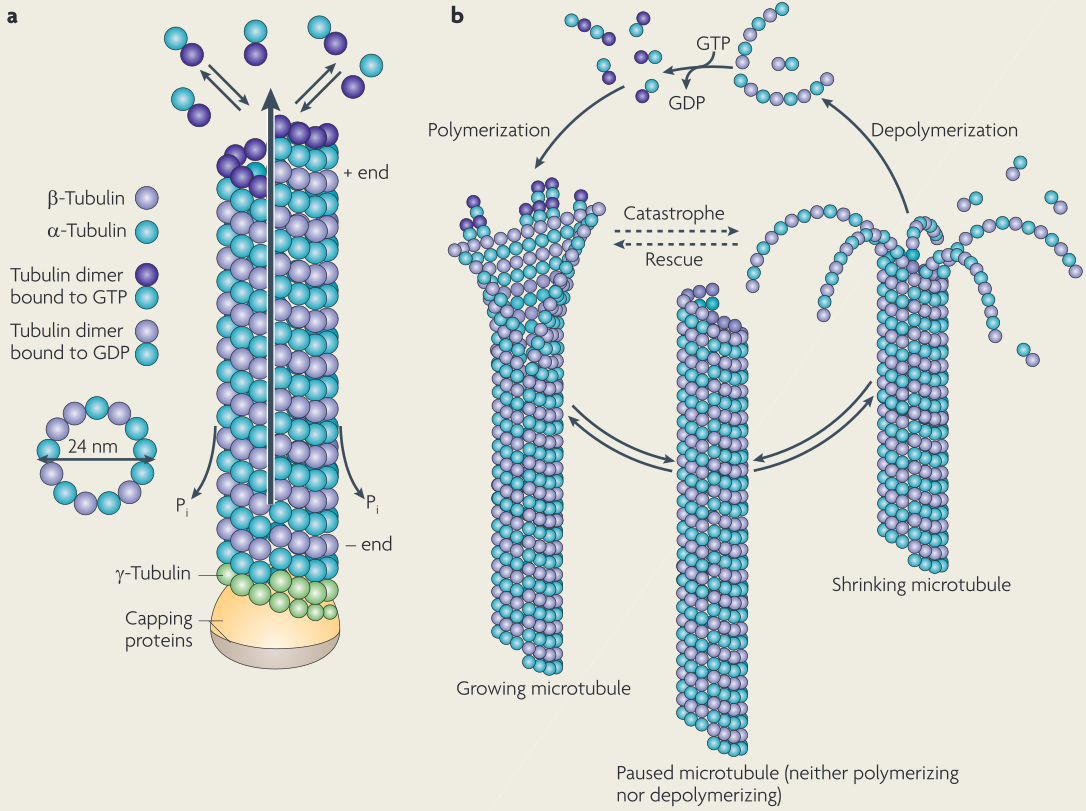
\includegraphics[width=0.9\linewidth]{images/MT.png}
  \caption[Microtubule structure]{Microtubule structure and
  its dynamic instability. Figure from \cite{Conde2009}.}
  \label{f:I-MT}
\end{figure}
The 
depolymerization process is characterized by protofilaments
bending outward and displaying a structure that looks 
like ram's horns (see Fig. \ref{f:I-MT}b).
GTP-bound tubulin can begin adding to the tip of the MT
again providing a new cap that protects against disassembly,
a process termed rescue.
MTs generate forces within cells via the stochastic 
switching between growth and shrinkage, also known
as dynamic instability
\cite{Carlier1981}. 
These forces contribute to 
several biological processes within cells including mitotic spindle formation and
chromosome segregation during cell division, maintenance
of cellular morphology and cytoskeleton, and intracellular
transport.
MTs have also been implicated in playing direct or indirect roles in signaling, information processing, and consciousness
and they are linked to cognitive diseases such as 
Alzheimer's disease.

The role of MTs in cell division makes them important targets
for cancer treatment. Since the rapidly dividing tumor
cells depend on MT during cell division, disruption of the
subtle MT stability balance, either by stabilization or destabilization, should hinder
the cell division process. Several available chemotherapeutic
agents act by stabilizing MT structure, such as taxanes 
and epothilones, or destabilizing it and preventing tubulin
polymerization, such as colchicine and vinca alkaloids. In both cases, cell division is arrested and the cells die by
apoptosis.
This cytotoxicity is not only limited to  cancer cells, but
also affects other rapidly dividing cells such 
as intestinal epithelium and bone marrow, leading to the 
known side effects of chemotherapy.


\section{Computational Methodology}
In this thesis, we simulated several
MT stabilizing agents and studied their
effects on tubulin and their free energies of 
binding. We also studied the stability of MTs
and their binding energetics at lateral and longitudinal inter-dimer interfaces. These stability studies related to the 
MT dynamic instability and mechanisms of disassembly. In these studies, we employed 
different computational techniques including;
similarity-based virtual screening, molecular docking, molecular dynamics simulations, 
Molecular Mechanics Poisson-Boltzmann (Generalized Born) Surface Area MM/PB(GB)SA
free energy calculations and 
Density Functional Theory (DFT) calculations
followed by population analysis employing the
\gls{qtaim}. In the remaining part of this section, we
will cover some of the basics of the methods
employed throughout the thesis.
The references that were primarily used in this section include
the books by Cramer \cite{Cramer2004} and Bader \cite{Bader1990}
and the online CHARMM tutorial \cite{CHARMM}. Other useful
reviews could be found in \cite{Adcock2006} and \cite{Karplus2002}. 

\subsection{Molecular Mechanics Force Fields}


\footnote{This section is based on section 2.2 from the textbook by Cramer
\cite{Cramer2004}} A force field is a collection of parameters and
equations used to calculate the potential energy 
of a system of atoms in molecular mechanics
simulations and geometry optimizations.
In calculating the potential energy of a system of atoms or molecules, several terms contribute
to the overall energy of the system. In molecular
mechanics, those terms represent either bonded interactions or non-bonded interactions.
Bonded interactions include atoms which are separated by three bonds or less, including bond stretching terms,
angle bending terms and torsional or dihedral
terms. Non-bonded interactions include atoms that are either non-bonded or farther than three bonds apart like van der Waals interactions and electrostatic interactions. With these contributions summed up over all 
interacting atoms, the overall force field
equation is:

\begin{equation}
\label{e:I-ff}
E_\text{total} = \sum E_\text{bond} + \sum E_\text{angle} + \sum E_\text{torsion} + \sum E_\text{electrostatic} 
+ \sum E_\text{vdW}
\end{equation}

We will briefly introduce each term and discuss
the corresponding formula.

\subsubsection{Bond Stretching}

In molecular mechanics force fields, the atoms
are treated as solid spheres attached by
springs where the potential energy can simply be calculated using the parameters of the springs
and Hooke's law. The bond stretching term 
is evaluated according to the following equation:
\begin{equation}
E_\text{bond} = \sum_{bonds} K_r
\left(r - r_{eq} \right)^2,
\end{equation}
where the sum runs through all the
bonds in the system, $K_r$ is
the force constant, $r_{eq}$ is
the equilibrium bond length
specific for each bond, and $r$ 
is the distance between the two bonded atoms. Values
of the force constant specific
for each bond is obtained from
either quantum mechanics
calculations or from experimental
data such as infrared stretching
frequencies. Equilibrium 
bond lengths could be obtained 
from high resolution 
crystal structure and microwave 
spectroscopy.
Although this harmonic potential 
is less accurate than 
the Morse potential in describing
bond stretching terms, it is 
much cheaper in terms of computations
and performs reasonably well
around equilibrium bond lengths
where the bond deformations are 
small.

\subsubsection{Angle Bending}

Following a similar principle,
the angle bending term of the
potential energy function could be 
evaluated according to the following harmonic potential:

\begin{equation}
E_\text{angle} = \sum_{angles} K_{\theta}
\left(\theta - \theta_{eq} \right)^2,
\end{equation}
where $K_{\theta}$ and $\theta_{eq}$
are the force constant and 
equilibrium angle associated with 
the three atoms in question, respectively, and $\theta$ is the actual
angle between the three bonded atoms. The sum runs through 
all the angles between bonded atoms
in the system and assigns a penalty for each deviation from equilibrium
angles.

\subsubsection{Torsions}

A torsional or dihedral angle $\phi$ between bonded atoms
ABCD is defined as the angle between bonds
AB and CD when they are projected into the
plane bisecting the BC bond. The rotation
of the BC bond changes the steric interactions
between A and D, altering the potential energy
of the system. This potential is periodic
and is often expressed as a cosine function
like the following form:
\begin{equation}
E_\text{torsion} = \sum_{torsions} \frac{V_{n}}{2}
\left[1+\cos(n\phi-\gamma)\right],
\end{equation}
where $V_n$ is the term amplitude, $n$ is the
periodicity, and $\gamma$ is the phase angle.
The parameters of the previous bonded potentials are usually
obtained from spectroscopic data of small
model compounds aided with \emph{ab inito} quantum
calculations.

\subsubsection{van der Waals Interactions}

This type of non-bonded interactions has two components, an
attractive component and a repulsive one. The attraction
comes from fluctuations in the electron cloud around
an atom giving rise to an instantaneous dipole which
induces a dipole in a nearby atom giving rise to 
attractive forces. The repulsion comes from overlap
of electron clouds at short distances. The two 
competing forces have different dependence on 
distance giving rise to a minimum in
the potential energy curve. 
\begin{figure}
  \centering
  \includegraphics[width=0.7\linewidth]{images/lj.eps}
  \caption[Lennard-Jones potential]{Lennard-Jones 
  potential curve showing optimum distances $r_{ij}^{*}$ and well depth $\varepsilon$. Units on axes are arbitrary.}
  \label{f:I-LJ}
\end{figure}
The curve is best described
via the Lennard-Jones potential shown in 
Fig. \ref{f:I-LJ}. The total potential
energy due to the van der Waals term is expressed in the following equation:
\begin{equation}
E_{vdW} = \sum_{i<j} \varepsilon \left[ \left(\frac{r_{ij}^*}{r_{ij}}\right)^{12} - 2\left(\frac{r_{ij}^*}{r_{ij}}\right)^{6} \right], 
\end{equation}
where $\varepsilon$ is the well-depth and $r_{ij}^*$
is the optimum distance specific for each pair of atoms, and
$r_{ij}$ is the distance between the atoms. Because
this pairwise energy function scales as $N^2$, where $N$ is the
number of atoms in the system , a typical cut-off
distance of 10 \r{A} is usually applied which 
reduces the number of calculations considerably. Since abrupt
decline of energy at the cut-off distance may introduce
discontinuities, a smooth switching function is usually 
applied.

\subsubsection{Electrostatic Interactions}

The second type of non-bonded interactions
is the electrostatic interaction between pairs of
atoms. If $\epsilon$ is the dielectric constant of the medium and
$r_{ij}$ is the distance separating two atoms
having charges $q_i$ and $q_j$, then the electrostatic
potential energy becomes;
\begin{equation}
E_{ele} = \sum_{i<j} \frac{q_i q_j}{\epsilon r_{ij}}
\end{equation}
Such a pairwise interaction would scale as $N^2$ which 
would become very demanding especially in periodic systems.
The application of cut-off distances is not as an attractive solution
as in the case of van der Waals interactions since 
electrostatic interactions decay in a much slower
fashion. In other words, the long-range component of the Lennard-Jones potential decays proportionally to $r^{-6}$
while electrostatic potential decays proportionally to $r^{-1}$.
A better alternative for evaluating long-range electrostatic potential in infinite periodic
systems is the Ewald sum technique. Through a reciprocal-space
technique for treatment of long-range interactions,
the total electrostatic interaction can be calculated to 
given level of accuracy with a scaling that is as
low as $N\text{log}N$ in the 
most favorable case (i.e. Particle-Mesh-Ewald). 

\subsection{Molecular Dynamics Simulations}

\footnote{This section is based on chapter 3 from the textbook by Cramer
	\cite{Cramer2004}} \gls{md} simulations belong to a group of computational 
methods often employed in the study of behavior and properties
of biological molecules. Molecular dynamics simply
provides a means, based on a potential energy function like
the one described above, of simulating the evolution 
of the phase-space trajectory of a molecular system with time. It is a deterministic method,
meaning that provided a point on the phase space trajectory of a molecular
system, the ``next'' point in time can be determined.
Statistical mechanics is at the core of molecular dynamics
simulations where the microscopic information provided
through the simulations is converted into macroscopic
properties.


Molecular dynamics simulations generate a sequence of points 
in the phase space as a function of time. These points are 
different conformations of the system at a particular 
thermodynamic state, belonging to a certain thermodynamic
ensemble. Since most of chemical processes take place under
constant temperature and pressure, the isothermal-isobaric
ensemble is often used for our molecular dynamics
simulations. In a certain statistical ensemble, the ensemble
average of any property $A$ which is dependent on positions
$\mathbf{p}$ and momenta $\mathbf{p}$ is expressed as follows:
\begin{equation}
\label{e:I-ensemble}
\left<A \right>_\text{ensemble} =  \iint A(\mathbf{p},\mathbf{q}) \rho (\mathbf{p},\mathbf{q})d\mathbf{p} d\mathbf{q}
\end{equation}
where $\rho(\mathbf{p},\mathbf{q})$ is the probability density
function of the system being at a particular phase space
point. This probability is dependent on the energy $E(\mathbf{p},\mathbf{q})$ associated
with the phase space point according to
\begin{equation}
\label{e:I-rho}
\rho(\mathbf{p},\mathbf{q}) = \frac{1}{Q}e^{-E(\mathbf{p},\mathbf{q})/k_{B}T}
\end{equation}
where $k_B$ is the Boltzmann's constant, $T$ is the temperature
and $Q$ is the partition function 
\begin{equation}
Q = \iint e^{-E(\mathbf{p},\mathbf{q})/k_{B}T}
d\mathbf{p} d\mathbf{q}
\end{equation}
which could be viewed as a normalization constant for
the probability density function $\rho$. 
Since the evaluation of these integrals requires knowledge about
all the possible microstates of a system, it is extremely
difficult to calculate.
In a molecular dynamics simulation, however, we are provided
with sequential points in time along the phase-space
trajectory. In this case we can calculate the time average of the
property of interest
\begin{equation}
\label{e:I-timeA}
\left< A \right>_{time}  = \lim_{\tau\to\infty} \frac{1}{\tau} \int_{t=0}^{\tau} A(t) dt
\end{equation} 
where $A(t)$ is the instantaneous value of the 
property $A$ given the positions and momenta at
time $t$, and $\tau$ is the simulation time.
In the limit of an infinite simulation time,
we can assume that the system will pass through all the
possible microstates within a certain thermodynamic
ensemble. 
This leads to one of
the most fundamental hypotheses of statistical mechanics, i.e the ergodic hypothesis. It states
that the time average equals the ensemble average:
\begin{equation}
\left< A \right>_{ensemble} = \left< A \right>_{time}
\end{equation}
However, it is impossible to run a simulation for
an infinitely long time and hence the limit in
Eq. \ref{e:I-timeA} can not be reached.
This limitation can be circumvented by
realizing that many points in the phase space
are negligible. Eq. \ref{e:I-rho} shows that
conformers having very high energies,
for instance due to substantial molecular deformations, will
have near-zero probabilities and hence
the integrand in Eq. \ref{e:I-ensemble}
will also be near-zero (as long as the
property $A$ does not approach infinity).
This integrand will thus contribute negligibly
to the property of interest and can be ignored
as it does not contribute to the property
expectation value. Starting with a reasonable,
preferably experimentally-determined,
structure, molecular dynamics provides
a suitable prescription for sampling important
phase space points (i.e. points having low energy and
high probability) which contribute most
to the property of interest. For a finite
number of phase space points, the 
expression in Eq. \ref{e:I-timeA} approximates
to
\begin{equation}
\left< A \right>_{time}  \approx \frac{1}{M}
\sum_{i=1}^{M} A(t_i)
\end{equation}
where $M$ is the number of times the property is
sampled during the simulation, which reflects
the number of important conformations sampled
from the trajectory.

Given the positions of atoms in a system which 
are preferably obtained from experiment, initial distribution
of velocities is assigned conforming to a certain temperature
$T$ to guarantee no overall momentum, i.e.
\begin{equation}
P = \sum_{i=1}^{N} m_i v_i = 0
\end{equation}
where the velocities $v_i$ are assigned randomly through
the Maxwell-Boltzmann distribution at a given temperature.
The probability of an atom $i$ having a velocity $v_{ix}$
in the $x$ direction is
\begin{equation}
p(v_{ix}) = \sqrt{\frac{m_i}{2 \pi k_B T}}
e^{-mv_{ix}^2/2k_BT}
\end{equation}
and the overall temperature of the system can be obtained
from the relationship
\begin{equation}
T = \frac{1}{3Nk_B} \sum_{i=1}^{N} \frac{|p_i|^2}{m_i}
\end{equation}
where $N$ is the number of atoms. Given this initial set of
positions and momenta, the trajectory is traced 
and positions and momenta are re-calculated
after every time step $\Delta t$ until the simulation time
is covered. Time steps are chosen so they are shorter than 
the fastest motion in the system, typically the
heavy-atom-hydrogen bond having a period of $10^{-14}$ s. However, with the application of a constraint
such that these bonds remain at a constant length,
using for instance the SHAKE algorithm, a time step as 
long as 2 fs can be used. The next challenge in molecular
dynamics is how the positions an momenta can be updated
after each time step. This is achieved through either of
the following integration algorithms.

\subsubsection{Verlet Algorithm}

The position after a time step $\Delta t$ can be expressed
using the Taylor series expansion:

\begin{equation}
\mathbf{q}(t+\Delta t) = \mathbf{q}(t) + \mathbf{v}(t)\Delta t + \frac{1}{2!} \mathbf{a}(t) (\Delta t)^2 + \frac{1}{3!} \frac{d^{3}\mathbf{q}(\tau)}{dt^3} \Big| _{\tau=t} (\Delta t)^3
+ ...
\end{equation}
where velocity $\mathbf{v}$ and the acceleration $\mathbf{a}$ represent the first and second time derivatives of the 
position vector $\mathbf{q}$. Evaluating the Taylor expansion 
corresponding to a reverse time step,
\begin{equation}
\mathbf{q}(t-\Delta t) = \mathbf{q}(t) - \mathbf{v}(t)\Delta t + \frac{1}{2!} \mathbf{a}(t) (\Delta t)^2 - \frac{1}{3!} \frac{d^{3}\mathbf{q}(\tau)}{dt^3} \Big| _{\tau=t} (\Delta t)^3
+ ...
\end{equation}
Summing the two equations and truncating at the second order
(which is equivalent to truncating at the third order
since it has a coefficient of zero) we get:
\begin{equation}
\mathbf{q}(t+\Delta t) = 2 \mathbf{q}(t) - \mathbf{q}(t-\Delta t) + \mathbf{a}(t)(\Delta t)^2
\end{equation}
Hence, the Verlet algorithm updates the position using only
the position and acceleration at time $t$ and the position
at time ($t-\Delta t$) without any explicit reference
to velocities. This makes the algorithm straightforward and
less computationally demanding, but it also lacks velocity 
information which is often required at least for
temperature control.

\subsubsection{The Leapfrog Algorithm}

As an alternative to the Verlet algorithm which lacks
explicit velocity information, the leapfrog algorithm
uses a Taylor series expansion about $(t+\Delta t/2)$
truncated at the second order as follows:
\begin{equation}
\label{e:I+dt}
\mathbf{q}\left(t+\frac{1}{2}\Delta t+\frac{1}{2}\Delta t\right) = 
\mathbf{q}\left(t+\frac{1}{2}\Delta t\right) + \mathbf{v}\left(t+\frac{1}{2}\Delta t\right)\frac{1}{2} \Delta t + 
\frac{1}{2!} \mathbf{a}\left(t+\frac{1}{2}\Delta t\right) \left(\frac{1}{2}\Delta t\right)^2
\end{equation}
and
\begin{equation}
\label{e:I-dt}
\mathbf{q}\left(t+\frac{1}{2}\Delta t-\frac{1}{2}\Delta t\right) = 
\mathbf{q}\left(t+\frac{1}{2}\Delta t\right) - \mathbf{v}\left(t+\frac{1}{2}\Delta t\right)\frac{1}{2} \Delta t + 
\frac{1}{2!} \mathbf{a}\left(t+\frac{1}{2}\Delta t\right) \left(\frac{1}{2}\Delta t\right)^2
\end{equation}
Subtracting Eq. \ref{e:I-dt} from Eq. \ref{e:I+dt}
we obtain
\begin{equation}
\mathbf{q}\left(t+\Delta t \right) = 
\mathbf{q}(t) + \mathbf{v}\left(t + \frac{1}{2} \Delta t\right)
\Delta t
\end{equation}
A similar expansion for $\mathbf{v}$ gives
\begin{equation}
\mathbf{v}\left(t+\frac{1}{2}\Delta t \right) = 
\mathbf{v}\left(t-\frac{1}{2}\Delta t \right) + \mathbf{a}\left( t\right)
\Delta t
\end{equation}
In this algorithm, the velocities are calculated 
at $(t+\Delta t/2)$ and are then used
to calculated the positions at $(t+\Delta t)$
and thus the velocities leap over positions and
then the positions leap over the velocity, hence the name.
Other integration algorithms also exist such as the
velocity Verlet and the Beeman's algorithm.

\subsection{Energy Calculations with MM/PB(GB)SA Algorithm}

This approach was first described by Kollman et al. in 2000 \cite{Kollman2000}.
After a molecular dynamics simulation of a ligand bound to 
a receptor protein is run in a solvent and in the presence of counterions, an equilibrated system of the ligand-receptor complex is obtained. 
A set of uncorrelated snapshots from the trajectory is then post-processed by removal of the solvent and counterions. The average free energy of each species, ligand, receptor or complex, is calculated according to the following equation:
\begin{equation}
\label{eq:VS-G}
\bar{G} = \bar{E}_{\text{MM}} + \bar{G}_{\text{PB(GB)SA}} - TS_{\text{MM}}
\end{equation}
where $\bar{E}_{\text{MM}}$ is the average molecular mechanical energy calculated according to Eq. \ref{e:I-ff}.
The term $\bar{G}_{\emph{PBSA}}$ refers to the solvation free energy obtained from the Poisson-Boltzmann (or generalized Born) equation for implicit solvent model and an estimate for the non-polar free energy via a surface area term,
vide infra. The
term $-TS_{\emph{MM}}$ represents the entropic component which involves translational, rotational and vibrational contributions. Vibrational contributions can be calculated via normal mode analysis where different conformations are minimized and the Hessian matrix is diagonalized, then vibrational entropies can be estimated from vibrational frequencies. After calculating the average free energies for the ligand, the receptor and the complex, the total average free energy of binding in solution equals:
\begin{equation}
\label{eq:VS-dG}
  \Delta{G} = \bar{G}_{\emph{complex}} - \bar{G}_{\emph{receptor}} - \bar{G}_{\emph{ligand}}
\end{equation}
We will give a brief introduction about the solvent effects
in the continuum model PB, GB and the surface area based method.
Extended discussions on continuum models can be found in chapter 11
of the text book by Cramer \cite{Cramer2004}.

\subsubsection{Poisson-Boltzmann Electrostatics}

The Poisson-Boltzmann equation describes
the electrostatic environment of a solute present in
an ion-containing solvent. It has the following 
form:
\begin{equation}
    \vec{\nabla}\cdot\left[\epsilon(\vec{r})\vec{\nabla}\Psi(\vec{r})\right] = -\rho^{f}(\vec{r}) - \sum_{i}c_{i}^{\infty}z_{i}q\lambda(\vec{r})e^{-z_{i}q\Psi(\vec{r})/k_BT} 
\end{equation}
where $\epsilon(\vec{r})$ represents the position-dependent dielectric, $\Psi(\vec{r})$ represents the electrostatic potential, $\rho^{f}(\vec{r})$ represents the charge density of the solute, $c_{i}^{\infty}$ represents the concentration of ion $i$ at a distance of infinity from the solute, $z_{i}$ is the valence of the ion, $q$ is the charge of a proton, $k_B$ is the Boltzmann constant, $T$ is the temperature, and $\lambda(\vec{r})$ is a factor for the position-dependent accessibility of position $r$ to the ions in solution. If the potential is not large, the equation can be linearized to be solved more efficiently.

\subsubsection{Generalized Born Electrostatics}

If the solute is treated as a set of spheres with 
an internal dielectric constant that is different from the 
external solvent, the generalized Born model
can offer an approximation to the exact linearized 
Poisson-Boltzmann equation with the following form:
\begin{equation}
    G_{s} = \frac{1}{8\pi}\left(\frac{1}{\epsilon_{0}}-\frac{1}{\epsilon}\right)\sum_{i,j}^{N}\frac{q_{i}q_{j}}{f_{GB}} 
\end{equation}
where
\begin{equation}
f_{GB} = \sqrt{r_{ij}^{2} + a_{ij}^{2}e^{-D}}
\end{equation}
and
\begin{equation}
 D = \left(\frac{r_{ij}}{2a_{ij}}\right)^{2}, \qquad a_{ij} = \sqrt{a_{i}a_{j}} 
\end{equation}
In the equation, $\epsilon_0$ is the permitivity of 
free space while $\epsilon$ is the solvent dielectric constant.
$q_i$ is the charge on atom $i$ and $r_{ij}$ is the distance
between atoms $i$ and $j$. The quantity $a_i$ is the effective
Born radius, reflecting its degree of burial within the
solute.

\subsubsection{Accessible Surface Area Based Method}

Contrary to the PB or GB models which only estimate the
enthalpic components of free energy, the accessible surface
area method gives the total free energy of solvation.
This is calculated as follows:

\begin{equation}
\Delta G_\text{SA} = \sum_{i=1}^{N} \sigma_i{\gamma_i}
\end{equation}
where $\gamma_i$ is the accessible surface area of atom $i$
and $\sigma_i$ is the solvation parameter of the same atom.
The solvation parameter is defined as the contribution 
of the atom to the free energy of solvation per unit surface area.
The free energy of solvation mounts to the change in free
energy upon transfer of the atom/molecule from the solvent
to vacuum (or other solvents) which is determined from the partition
coefficients of the compounds between different media. 

\subsection{Quantum Theory of Atoms in Molecules}

The quantum theory of atoms in molecules (QTAIM) is a theory that was
developed by Richard Bader and his research group at
McMaster University over the course of decades.
The theory characterizes atoms and bonds in a molecular 
structure based on the topology of the electron density.
A molecular structure is characterized by stationary points of the
electron density together with the gradient paths of the 
electron density that originate and terminate at these points.

According to quantum mechanics, the nuclei of atoms in molecular
structures act as point attractors immersed in a cloud of negative charge.
The distribution of the negative charge in space around the nuclei
is described by the electron density distribution function $\rho(\mathbf{r})$
where $\mathbf{r}$ is the space coordinates of a single electron. The
charge density is calculated through the following equation:
\begin{equation}
\rho (\mathbf{r}) = N \int d\tau\,\psi^*(\mathbf{x})\psi(\mathbf{x})
\end{equation} 
where $N$ is the number of electrons, $\tau$ represents the spin coordinates
of all electrons and the Cartesian coordinates of all electrons but one, and
$\psi$ is the state function expressed in $\mathbf{x}$ which is the 
collection of electronic space and spin coordinates. 

\begin{figure}
  \centering
  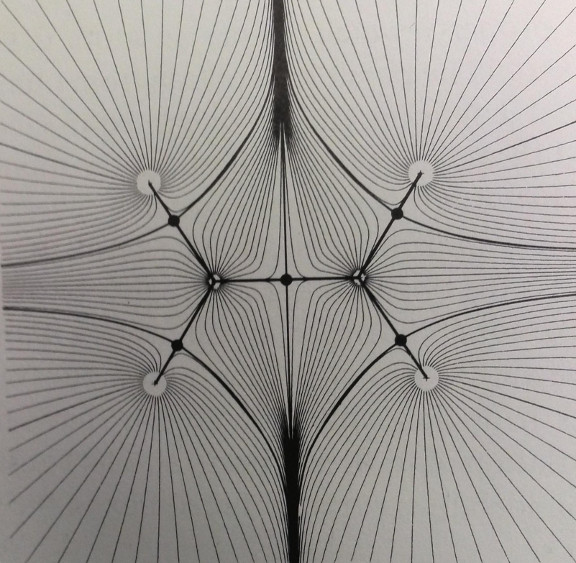
\includegraphics[width=0.55\linewidth]{images/aim.jpg}
  \caption[A map of the electron density gradient vector field]{A map of the electron density gradient vector 
  	field for the plane containing
  the nuclei of the ethene molecule.
  Each line represents a trajectory traced out by
  the vector $\mathbf{\nabla}\rho(\mathbf{r})$. Image adapted from
  \cite{aimplot}.}
  \label{f:Intro-aim}
\end{figure}

Each topological feature of the charge density function,
including maxima, minima, and saddle points, is characterized by a point
in space called a critical point, denoted by the vector $\mathbf{r_c}$. This is a point in which the first
derivative of the density function is zero, i.e. $\mathbf{\nabla} \rho(\mathbf{r})=0$.
The gradient is evaluated as follows:
\begin{equation}
\mathbf{\nabla} \rho = \mathbf{i} \frac{\partial \rho}{\partial x} + 
\mathbf{j} \frac{\partial \rho}{\partial y} + 
\mathbf{k} \frac{\partial \rho}{\partial z}
\end{equation}
Whether the function has a maximum or a minimum at a stationary point is
dictated by the second derivative, i.e. the curvature, at that point. 
The second derivative of the charge density function 
being the trace of the Hessian matrix
is expressed as follows:
\begin{equation}
\mathbf{\nabla}^2 \rho = \mathbf{\nabla}. \mathbf{\nabla} \rho = 
 \frac{\partial^2 \rho}{\partial x^2} + 
\frac{\partial^2 \rho}{\partial y^2} + 
 \frac{\partial^2 \rho}{\partial z^2}
\end{equation}
The principal axes and their corresponding curvatures at the critical points
are obtained as the eigenvectors and the corresponding eigenvalues in the 
diagonalization of the Hessian matrix of $\rho(\mathbf{r_c)}$.
A critical point could thus be characterized by two values; the rank ($\omega$)
and the signature ($\sigma$). The rank is the number of non-zero eigenvalues
or curvatures of $\rho$ at the critical point, and the
signature is the algebraic sum of the signs of the eigenvalues.
There are four different combinations of ($\omega$,$\sigma$) for
four different types of critical points:

\begin{itemize}
 \item ($3,-3$): where all curvatures are negative, signifying a local maximum in $\rho$. This 
usually indicates the position of the nuclei or the atoms, thus called atomic 
critical point.

\item ($3,-1$): where two curvatures are negative indicating two maxima 
and one is positive indicating a minimum. This occurs between two neighboring atoms and defines a bond between them, thus called a bond critical point.

\item ($3,+1$): where two curvatures are positive indicating two minima 
and one is negative indicating a maximum. This point occurs in the middle 
of several bonds forming a ring, thus called a ring critical point.

\item ($3,+3$): where all curvatures are positive indicating minima. This
is found between several points that form a cage and thus called cage critical point.
\end{itemize}

Fig. \ref{f:Intro-aim} shows a map of the gradient vector field of the electron
density $\mathbf{\nabla}\rho(\mathbf{r})$ at the plane of the nuclei in the ethene molecule. The figure
shows the trajectory lines that terminate at the nuclei (the small circles).
The set of trajectories that terminate at a given nucleus represent the basin of that nucleus. The figure also shows the sets of trajectories
which terminate and originate at bond critical points (denoted by dots).

\section{Scope of Thesis}
In the next chapters, our analysis of the dynamic instability of microtubules
and associated chemotherapeutic agents is presented. In Chapter \ref{TVS},
the results of virtual screening  for novel microtubule
stabilizing agents based on similarity fingerprints and structure-based 
design are presented. In Chapter \ref{lankacidin}, it is shown how the novel hits lead to
the prediction of the mechanism of antitumor action of lankacidin group
antibiotics and how this was confirmed experimentally. In Chapter \ref{HB},
analysis of different methods of estimation of hydrogen bond energies
is performed and the parameters and descriptors needed for estimation
are provided. These parameters and descriptors are used in Chapter
\ref{THB} to estimate hydrogen bonds between tubulin dimers 
across lateral and longitudinal interfaces. Finally, Chapter \ref{ligHB}
presents an atomistic simulation of a complete microtubule model
followed by a detailed per-residue MM/GBSA analysis which unravels the
driving force for microtubule disassembly.

\chapter{Similarity-Based Virtual Screening for Microtubule Stabilizers Reveals Novel Antimitotic Scaffold}   
\label{TVS}

\section{Summary}

Microtubules are among the most studied and best characterized cancer targets identified to date. Many microtubule stabilizers have been introduced so far that work by disrupting the dynamic instability of microtubules causing mitotic block and apoptosis. However, most of these molecules, especially taxol and epothilone, suffer absorption, toxicity and/or resistance problems. Here we employ a novel similarity-based virtual screening approach in the hope of finding other microtubule stabilizers that perform better and have lower toxicity and resistance. Epothilones, discodermolide, eleutherobin and sarcodictyin A have been found to compete with taxanes for the $\beta$-tubulin binding site, which suggests common chemical features qualifying for that. Our approach was based on similarity screening against all these compounds and other microtubule stabilizers, followed by virtual screening against the taxol binding site. Some novel hits were found, together with a novel highly rigid molecular scaffold. After visual manipulations, redocking and rescoring of this novel scaffold, its affinity dramatically increased in a promising trend, which qualifies for biological testing.

\let\thefootnote\relax\footnote{A version of this chapter was published as: 
A. T. Ayoub, M. Klobukowski, and J. Tuszynski, ``Similarity-based virtual screening for microtubule stabilizers reveals novel antimitotic scaffold,'' \emph{Journal of Molecular Graphics
and Modelling}, vol. 44, 188-196, 2013} 

\section{Introduction}
\label{s:VS-Intro}

Cancer is characterized by uncontrolled growth of cells within certain tissues that could spread to other tissues through metastasis. One of the most important cancer drug targets is the structural protein tubulin, the building block of microtubules. Microtubules are long filamentous tube-shaped protein polymers required in cells, among numerous other roles, for transport of vesicles and structural support
\cite{Hayden1990}. 
During the anaphase of the mitotic division, microtubules play the role of separating chromosomes to the poles of cell preceding telophase. Proper dynamics of microtubules, in terms of the delicate balance between catastrophe and rescue phases, are crucial for these mitotic phases to complete
\cite{Hayden1990}. 
Taxol and other anticancer \glspl{MSA} work by stabilizing the microtubules and thus disrupting their required dynamic instability, which leads to mitotic arrest followed by apoptosis
\cite{Schiff1979,Schiff1980}. 
The binding site of taxol was correctly identified to be in the $\beta$-tubulin of the $\alpha\beta$-tubulin heterodimer and was elucidated via electron crystallography and
photoaffinity labeling
\cite{Nogales1998,Rao1995,Rao1999}. 
Among the recognized MSAs are also epothilone, discodermolide, sarcodictyin and eleutherobin, all of which have been shown to compete with taxol for the $\beta$-tubulin binding site
\cite{Bollag1995,Hamel1999,Kowalski1997,Buey2005}. 
Also, laulimalide, which is an MSA, was shown to have affinity toward the taxol binding site 
\cite{Pineda2004,Khrapunovich-Baine2011} but its primary binding location has been shown to differ from that for taxol
\cite{Bennett2010}. 
Fig. \ref{f:VS-MSAs}
shows the two-dimensional structures of these molecules. Most of these MSAs, however, suffer from some solubility, toxicity and/or drug resistance problems
\cite{Orr2003,Natarajan2012,Singla2002,Hopper-Borge2009} revealed in pre-clinical and clinical trials. This strongly motivates the search for novel tubulin-binding agents that may be able to provide a better pharmacokinetic profile and evade the resistance caused by mutations or cellular efflux pumps. Several studies have been conducted to find out a common pharmacophore for the MSAs that compete with taxol for the binding site and some models have been presented
\cite{Ojima1999,He2000,Giannakakou2000}. 
However, the lack of definitive data regarding the bioactive conformation of some of these ligands, besides the high structural complexity of most of them poses some questions regarding the reliability of these pharmacophore models in virtual screening. Therefore, we employed another approach in this study, which is the similarity-based approach, for filtering large sets of molecules, instead of the pharmacophore approach. We also employed docking and virtual screening techniques supported by Tanimoto similarity
\cite{Nikolova2003} in the hope of finding new scaffolds for tubulin-binding agents that can strongly bind to the taxol binding site whilst having better molecular properties. For a pair of similar molecules A and B, Tanimoto similarity coefficient $J(A,B)$ is defined as

\begin{equation}
J(A,B) = \frac{|A \cap B|}{|A \cup B|}
\label{eq:T}
\end{equation}

which is the ratio between the intersection and the union of the fingerprints
of both molecules.

\begin{figure}[h]
\centering
\subfloat[Epothilone A]{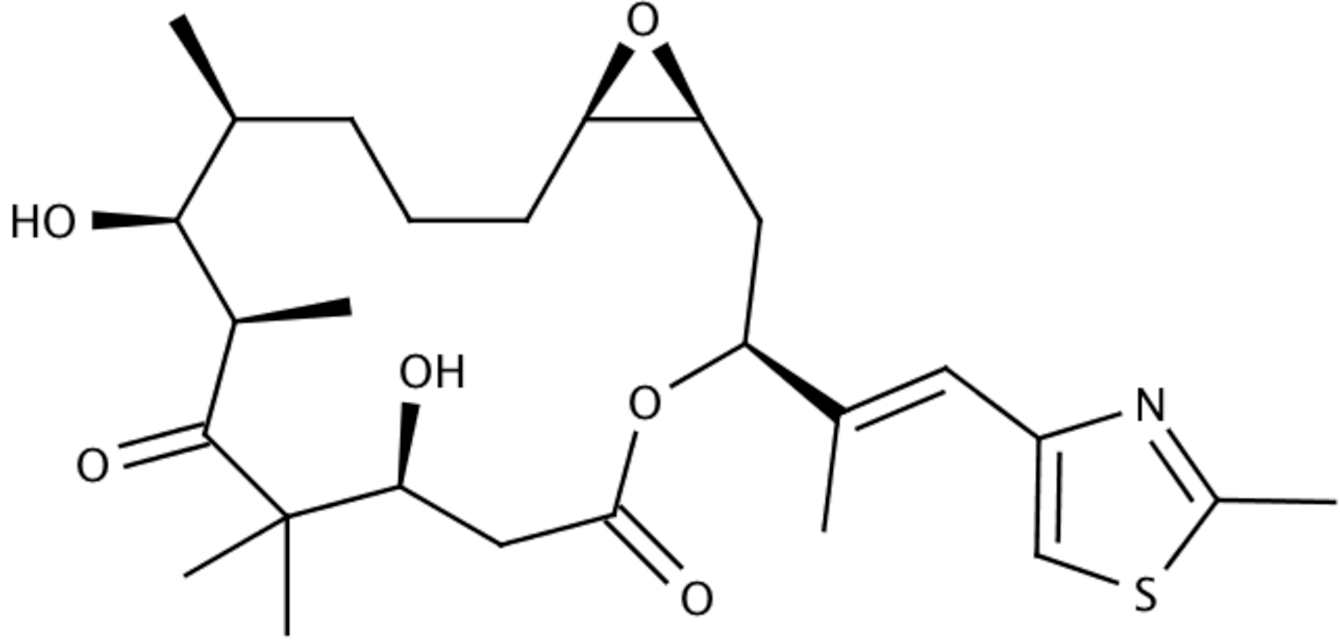
\includegraphics[width=4.6cm]{images/EpoA.pdf}}
\hspace{0.2cm}
\subfloat[Paclitaxel]{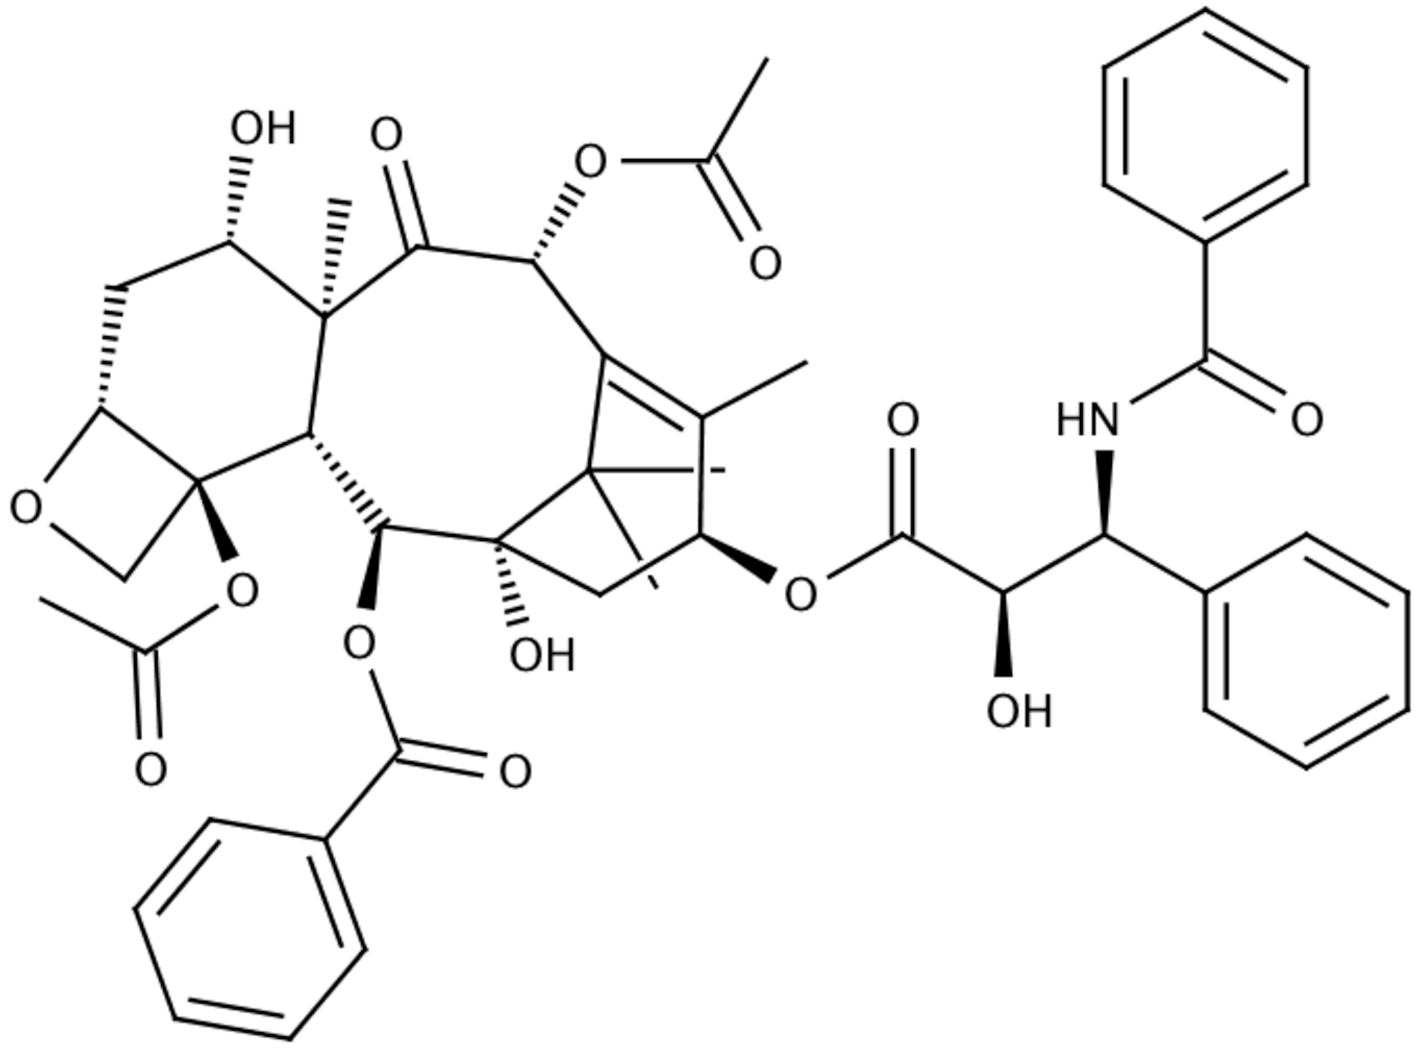
\includegraphics[width=5cm]{images/Paclitaxel.pdf}}
\hspace{0.2cm}
\subfloat[Eleutherobin]{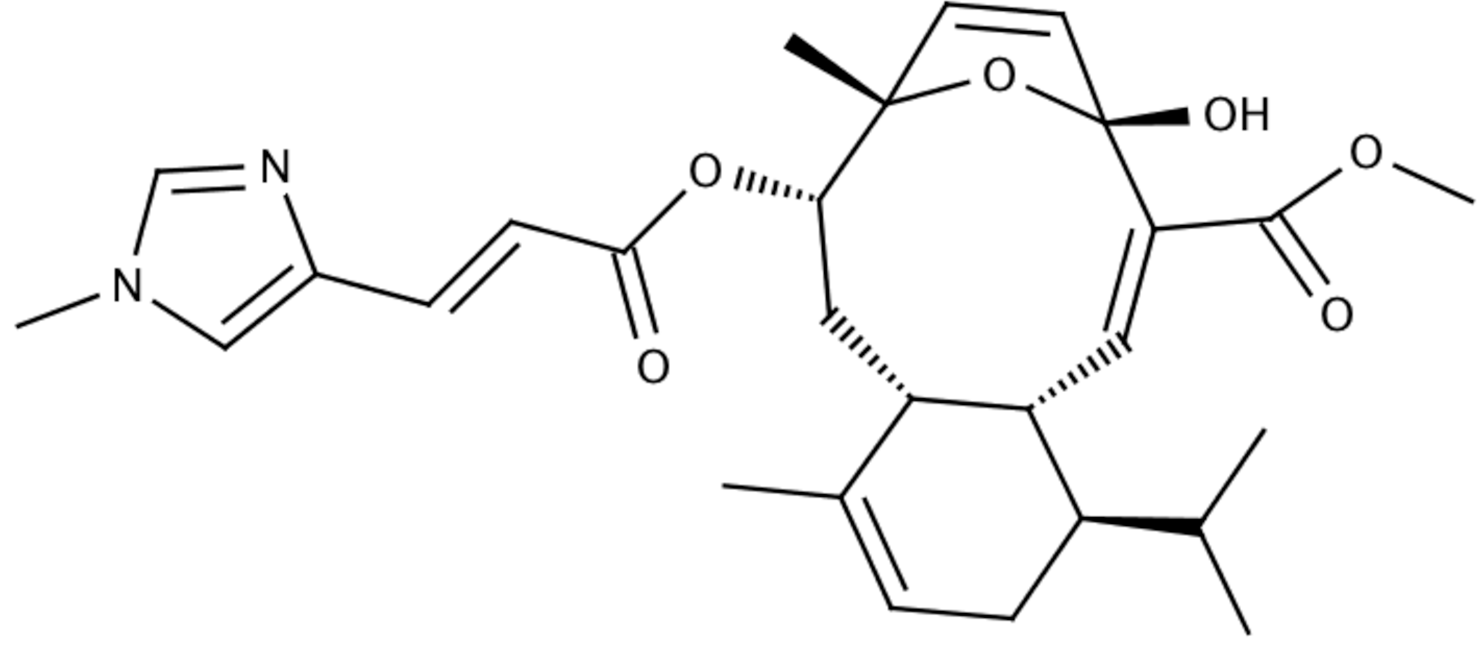
\includegraphics[width=5.5cm]{images/SarcodictyinA.pdf}}
\\
\subfloat[Discodermolide]{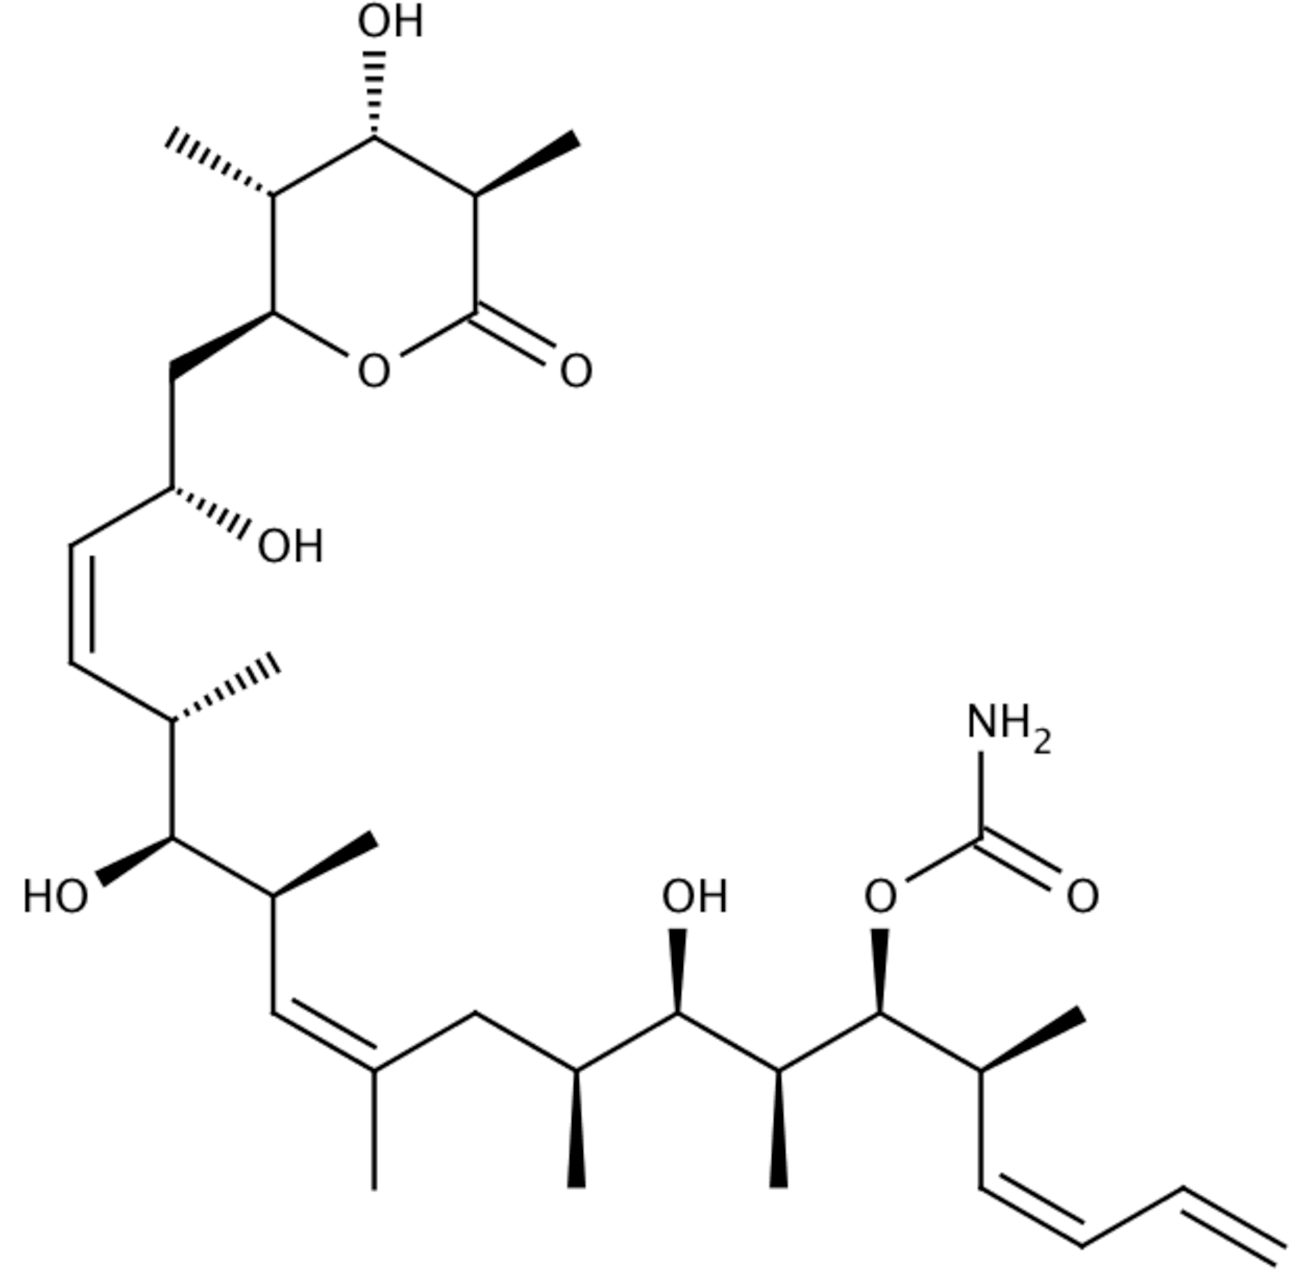
\includegraphics[width=4.1cm]{images/Discodermolide.pdf}}
\subfloat[Sarcodictyin A]{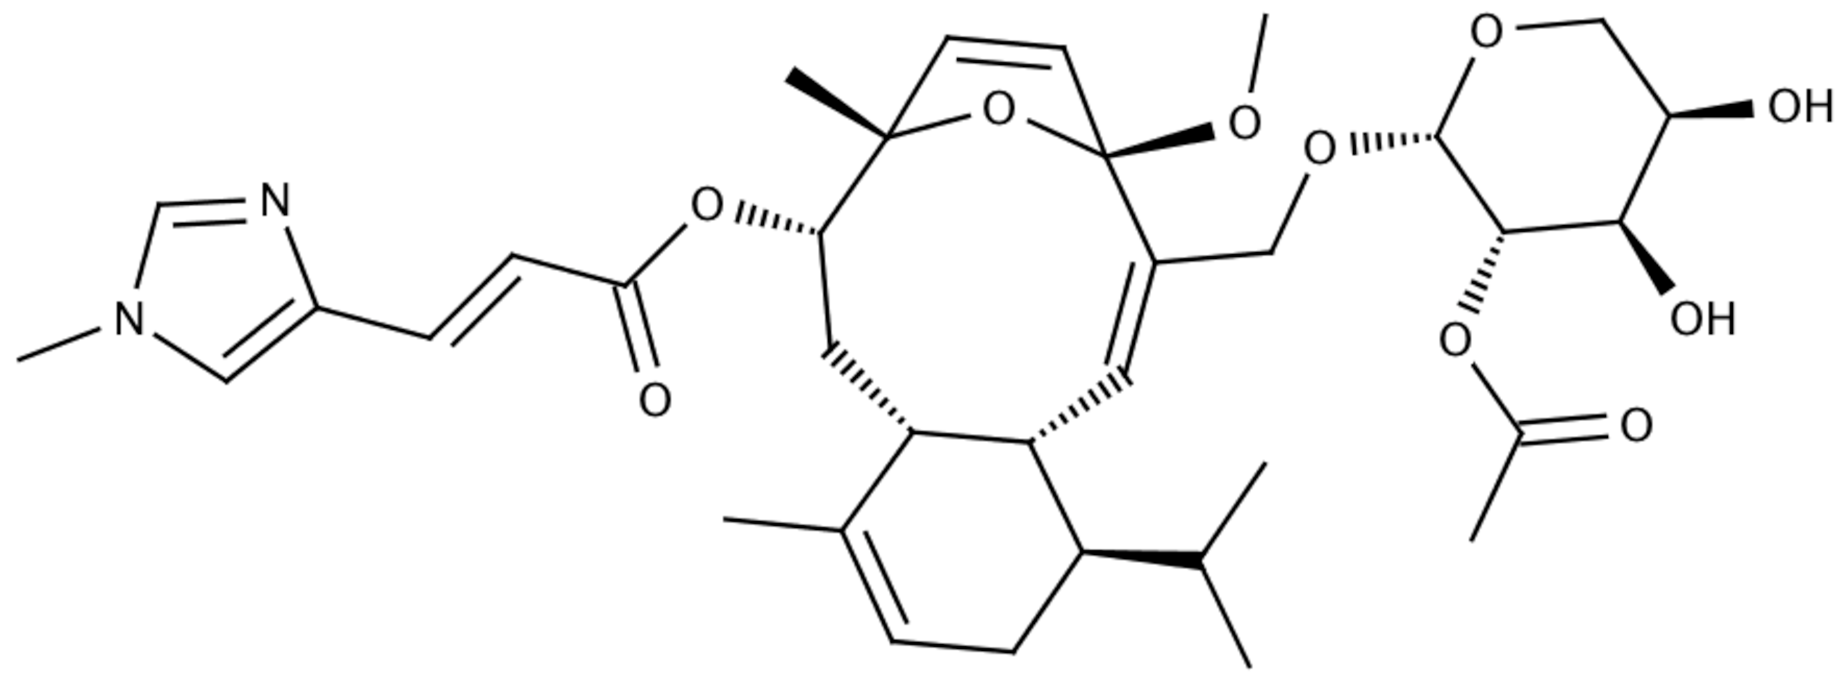
\includegraphics[width=5.1cm]{images/Eleutherobin.pdf}}
\hspace{0.2cm}
\subfloat[Laulimalide]{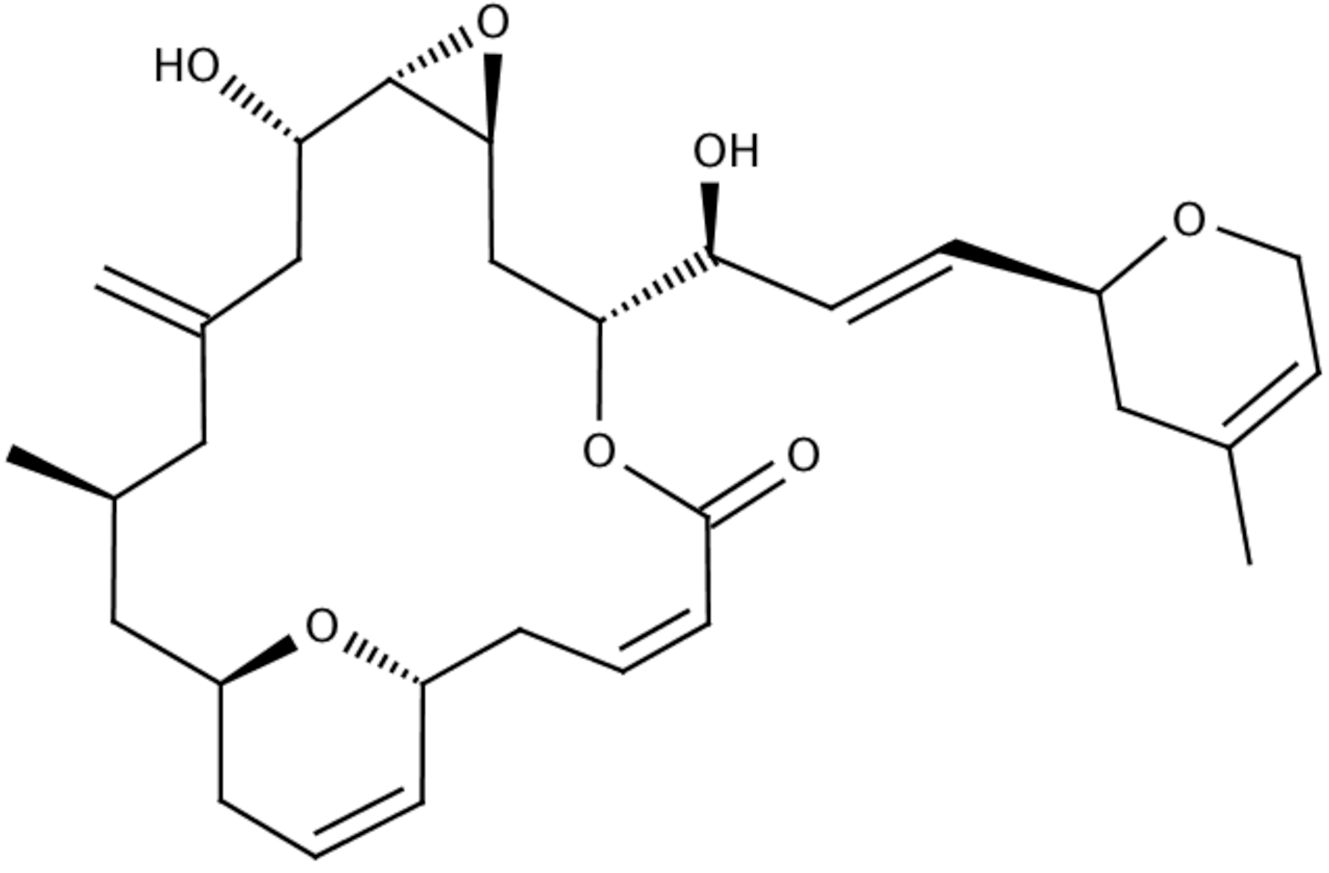
\includegraphics[width=4.4cm]{images/Laulimalide.pdf}}
\caption[Structures of microtubule stabilizing agents]{Structures of microtubule stabilizing agents that have affinity towards the taxol binding site on $\beta$-tubulin.}
\label{f:VS-MSAs}
\end{figure}


\section{Computational Methods}
\label{s:VS-Methods}

\subsection{Filtering PubChem Compound Library}
\label{ss:VS-Methods_Filtering}

As explained earlier, paclitaxel, epothilone A, discodermolide, sarcodictyin A, eleutherobin and laulimalide all have affinities toward the taxol binding site 
\cite{Bollag1995,Hamel1999,Kowalski1997,Buey2005,Pineda2004,Khrapunovich-Baine2011}. 
Based on that, we considered the ensemble of chemical features represented in these molecules as being representative of most of the chemical features required for binding to the taxol binding site. Hence, similarity with any of these six compounds was used as a criterion for filtering the compound database. The PubChem compound library, which is composed of nearly 33 million chemical entities, was screened against each of these six compounds separately to filter all the molecules that are at least 80\% similar to the query molecules based on the Tanimoto coefficient similarity metric \cite{Nikolova2003}. This threshold was chosen based on a trade-off between
the need to retain as large a number as possible to avoid false negatives
and the need to filter out as large a number as possible to increase the efficiency and speed.
The filtered molecules were then subjected to another filtering step based on Lipinski's rule of five that is widely accepted as a criterion from a pharmacological usefulness viewpoint
\cite{Lipinski2001}. The rule states that orally active drugs should have no more
than one violation of the following criteria: 1) no more than 5 hydrogen bond donors, 2) no more than 10 hydrogen bond acceptors, 3) a molecular mass
less than 500 daltons, and 4) an octanol water partition coefficient (log $P$) 
of less than 5.

The filtered molecules based on the six query structures were then combined together to give a library of 1591 molecules. Duplicates were deleted, the library was clustered and a diversity subset was selected based on
90\%
Tanimoto similarity to avoid having to evaluate molecules that are almost identical in structure. We ended up creating a library of 645 molecules that satisfy all of the above criteria and are ready for docking. We have added epothilone A as positive control. The 646 molecules were then docked into the taxol binding site using AutoDock 4.2
\cite{Morris2009}. Details of the filtration process are depicted in Fig.
\ref{f:VS-flowchart}. The Lamarckian genetic algorithm, which is a hybrid genetic algorithm with local search, was used for docking, with a maximum of 3 million runs of energy evaluations in a population size of 500 and a maximum of 50,000 generations. Docking poses were clustered based on a root-mean-square tolerance of 2.0 ˚A and the results were ranked based on the lowest energy in the largest cluster.
\begin{figure}
  \centering
  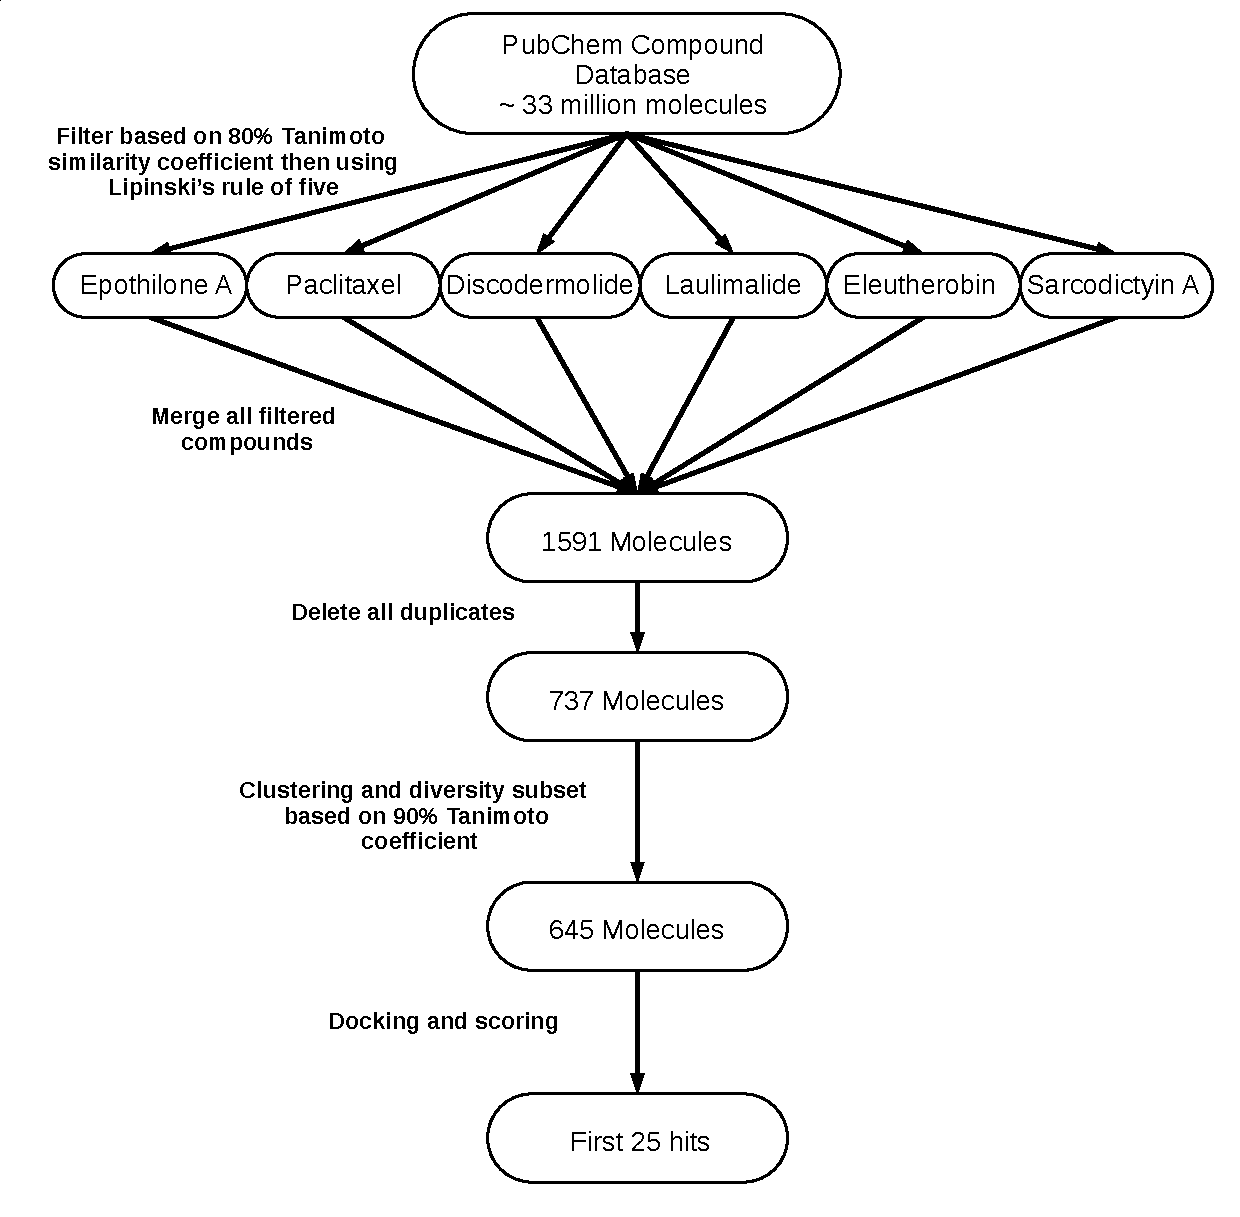
\includegraphics[width=0.6\linewidth]{images/Flowchart}
  \caption[Filtration scheme]{Filtration scheme of the PubChem Compound Library of $\sim$ 33 million molecules preceding docking.}
  \label{f:VS-flowchart}
\end{figure}

The top 25 hits were assessed for novelty of the scaffold and the
best candidate was modified visually. MarvinSketch 5.10.3, 2012 (ChemAxon) was used for drawing, displaying and characterizing chemical structures. Avogadro 1.0.3 was also used to assist in visualization and for energy minimization of the structures prior to docking
\cite{Hanwell2012}.
The best candidate from the virtual screening run was modified and several functional groups were added to different sites in the molecule to optimize the ligand-receptor complex based on visual inspection of the complex structure. The modified
molecules were then redocked into the taxol binding site. The visual modification and redocking steps were repeated five times until the derivatives showed highest affinity and no further improvements were being generated. Hybridization between the best scoring hits in each run was utilized to optimize the results in the subsequent run.

\subsection{Preparing Receptor for Docking}
\label{ss:VS-Methods_recPrep}

The receptor, tubulin, was obtained from the crystal structure 1TVK from the Protein Data Bank. 1TVK was preferred over 1JFF and 1TUB because of its high resolution (2.89 \r{A} as compared to 3.50 \r{A} and 3.70 \r{A}, respectively). The molecule was minimized using AMBER 12
\cite{case2012}
to relieve any unfavorable interactions that may result from crystal packing. The receptor was parameterized according to the AMBERff99SB force field
\cite{Hornak2006}. 
Hydrogen atoms were added to the protein based on the built-in AMBER residue templates, missing fragments were capped and residue His227 was kept in the deprotonated state
\cite{Nettles2004}. 
The Antechamber module of AMBER 12 package was used for parameterizing the ligands (epothilone, GDP and GTP) via the general AMBER force field
\cite{Wang2004}
and atomic partial charges were assigned using the AM1-BCC method
\cite{Jakalian2002}. 
The complex was built using the \emph{tleap} module of AMBER which was also used to neutralize the complex by addition of 18 sodium ions followed by extra 22 sodium and chloride ions to adjust ion concentration to 100 mM. The complex was solvated through a truncated octahedral box of the TIP3P water model that extended 
12 \r{A} in each direction. The model was minimized using AMBER 12 in a series of steepest descent and conjugate gradient steps. The minimized structure was then processed for docking; the $\alpha$-tubulin subunit
was deleted together with the solvent and all the ligands as they play no role in binding to the identified location on $\beta$-tubulin. Only the $\beta$-subunit was used for docking, at the epothilone binding site, which is the same as the taxane binding site. AutoDock Tools 4.2 was used to process the receptor
\cite{Morris2009}. 
The grid box for docking was centered around the crystallized epothilone structure in the binding site of 1TVK and was given the dimensions of $58 \times 58 \times 58$ grid points and was ready for docking. The software VMD was used for visualizing molecular dynamics (MD) trajectories
\cite{Humphrey1996}.

\subsection{Rescoring the best hits using MM/PBSA}
\label{ss:VS-Methods_rescoring}

Five of the six query molecules that were used for the similarity-based filtering (see Fig. 
\ref{f:VS-flowchart}) plus three of the highest-scoring hits that were obtained from the consecutive modification/redocking runs had their binding energies rescored using \gls{mmpbsa} approach that was introduced by Kollman et al.
\cite{Kollman2000}. 
This approach has been applied successfully in predicting the binding energies of many protein-ligand complexes 
\cite{Wang2001,Barakat2010,Lepsik2004,Brown2006,Hou2007}. 
Building on the success of these previous trials, we first rescored the five test molecules that interact with the taxol binding site with available experimental binding energies, namely discodermolide, eleutherobin, epothilone A, paclitaxel and sarcodictyin A, to verify the predictive power of the method through a linear fit. We neglected laulimalide because there was no available experimental data regarding its binding to the taxol binding site. Then we ran the same protocol with the highest-scoring hits to confirm the ranking as well as the binding energies
predicted by the docking algorithm.

All the ligand-receptor complexes were subjected to molecular dynamics simulation to obtain an equilibrated system. We used only the $\beta$-tubulin subunit for the simulations because the $\alpha$-subunit is not involved in binding and to save computational time. The simulations were performed using AMBER 12 package
\cite{case2012} following the same procedures as described in Sec. \ref{ss:VS-Methods_recPrep}. 
The GDP molecule that is normally attached to $\beta$-tubulin in the 1TVK structure was also parameterized following the same approach as other ligands and was docked into its binding site when forming the complexes to make the model as realistic as possible. The ligand-receptor complexes were built using the \emph{tleap} module of AMBER and were solvated with a truncated octahedral box of TIP3P water model extending 12 \r{A} in each direction. The charge was neutralized by the addition of 18 sodium ions, and then 22 sodium and chloride ions were added to adjust the ion concentration to 100 mM which mimics cellular conditions.
Each complex was then minimized without SHAKE on hydrogen and with very strong restraints on the protein through 500 steepest descent runs followed by 500 conjugate gradient steps. This was to relieve any unfavorable hydrogen contacts caused by the addition of hydrogen by \emph{tleap}. Then, the complexes were minimized once more without restraints or SHAKE through 2000 steps of steepest descent followed by 2000 steps of conjugate gradient to remove any other unfavorable contacts. The complexes were then subjected to 20 ps of heating using Langevin thermostat to 300 K at constant volume under SHAKE and restraints on the protein. This was followed by 200 ps of density equilibration at constant pressure with SHAKE on hydrogen but without restraints on the protein. Each complex was then taken through a production phase of 11 ns under constant pressure with the same settings as the previous density equilibration step. All the simulations were performed under periodic boundary conditions using Particle-Mesh-Ewald method for treating long-range electrostatics and Langevin thermostat for temperature control. Coordinates were recorded every 2 ps in the production run to ensure that the snapshots are uncorrelated. Total energy, temperature, density and \gls{rmsd} of the complexes were then checked for equilibration. Complexes were then subjected to an MM/PBSA calculation in AMBER 12 to calculate the binding enthalpy under an ionic strength of 100 mM and an internal and external dielectric constants of 1.0 and 80.0, respectively. Although computationally very demanding, the entropies of the solutes were estimated using
normal mode analysis in order to be able to calculate the total $\Delta G$ of the molecules and compare them to available experimental values as a check of the predictive power of the method in reproducing experimental data and hence being reliable in predicting the binding energy of the newly proposed ligands.

\subsection{Prediction of Physicochemical Properties}
\label{ss:VS-Methods_physico}

The compounds that showed high affinities during the docking/rescoring runs were checked for their physicochemical parameters. ADMET Predictor software
\cite{ADMET} 
was used for calculation of such parameters. This software
uses predictive neural networks ensemble
models with 2D and 3D descriptors. Parameters such as partition coefficient (log P), distribution
coefficient (log D), \gls{Peff}, and \gls{FaSSIF} were calculated. Potential toxicity was also assessed by the same software.

\section{Results and Discussion}
\label{s:VS-Results}

\subsection{Results of Virtual Screening}
\label{ss:VS-Results_VS}

As described previously in Fig.
\ref{f:VS-flowchart}, 
the similarity-based filtering of the $\sim$ 33 million molecules yielded 645 molecules. These molecules, together with epothilone A used as a positive control,
were docked with $\beta$-tubulin as described in Sec.
\ref{ss:VS-Methods_Filtering}. 
After ranking the docking results based on the lowest energy of the largest cluster, the best-scoring 25 molecules were examined. Before listing the results, it is worth mentioning that most of the highest scoring molecules are expected to be well-known and probably patented molecules. The approach that we are following, i.e. the similarity approach, retains molecules that are similar to active ones, including their patented analogs. If these analogs occur on top of the list, this is expected. Our main objective it to identify novel scaffolds, among these top hits, that can be modified to generate better ligands. The virtual screening algorithm predicted the first 25 hits to be strong tubulin binding agents spanning a binding
energy from $-10.03$ kcal/mol for the best hit (ligand PubChem CID of 10718437) to $-9.02$ kcal/mol for the worst one (ligand CID of 643649). 
To prove the efficiency of the docking algorithm in predicting active molecules, we will discuss the first five hits. From SciFinder, we found that the best hit, with CAS Registry Number of 198475-16-0, is an epothilone analog that was shown by Su et al. to have efficacy against cancer cell lines as a microtubule stabilizer
\cite{Su1997}. 
The second hit, CAS 219990-00-8, also has an activity against tubulin, similar to that of epothilone, and was patented by Vite et al. (patent number WO 9902514) and Francis Lee (WO 2002066038) for treatment of hyperproliferative cellular disease and refractory tumors, respectively. The third hit, which is a laulimalide analog with CAS of 1049737-16-7, was shown by Mooberry et al. to possess potent antiproliferative activity due to microtubule stabilization
\cite{Mooberry2008}. 
The fourth hit, CAS 220889-57-6, is an epothilone analog proven active by Lam et al.
\cite{Lam2012}.
Finally, the fifth hit, CAS 252917-46-7, was shown by Hardt et al. to be a potent epothilone analog
\cite{Hardt2001}.
In fact, all the top 25 hits, except for five novel ligands, represent compounds that have experimentally been shown to have tubulin stabilizing activities, which proves the reliability of our docking algorithm in determining active molecules. 

The five novel hits found in virtual screening are presented in 
Tab \ref{t:Vs-TopHits}. 
and compared to the positive control, epothilone A. The first of these five molecules, molecule 53 (CID 44333743), was shown by Sefkow et al. to have weak cytotoxic activity against the L 929 mouse fibroblast cell line, but was not patented
\cite{Sefkow1998}. 
\begin{table}
\centering
\caption[Binding energies of the five novel hits]{Binding energies of the five novel 
  hits obtained in the virtual screening run, plus the positive control, epothilone A.}
  \label{t:Vs-TopHits}  
  \begin{tabular*}{\linewidth}{@{\extracolsep{\fill}}>{\centering\arraybackslash}m{0.8cm}>{\centering\arraybackslash}m{0.8cm}>{\centering\arraybackslash}m{4.5cm}>{\centering\arraybackslash}m{1cm}}
    \toprule
    Rank & ID\textsuperscript{\emph{a}} & 
    Molecule & $\Delta{E}$\textsuperscript{\emph{b}}\\
    \midrule
    \\
    6  & 53 &
    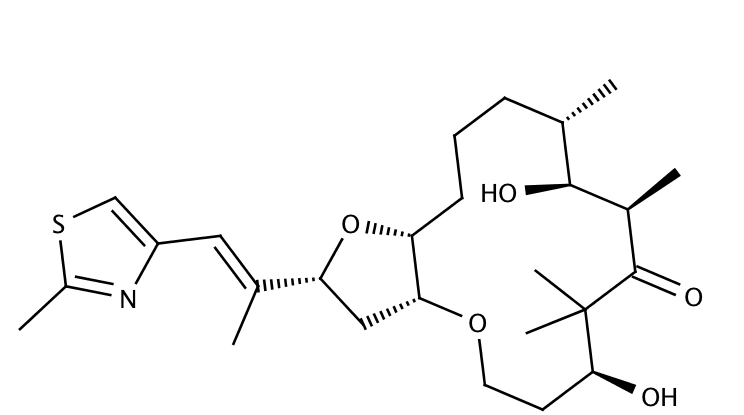
\includegraphics[width=4cm]{images/CID_44333743.png} & -9.58\\
    17 & 70 & 
     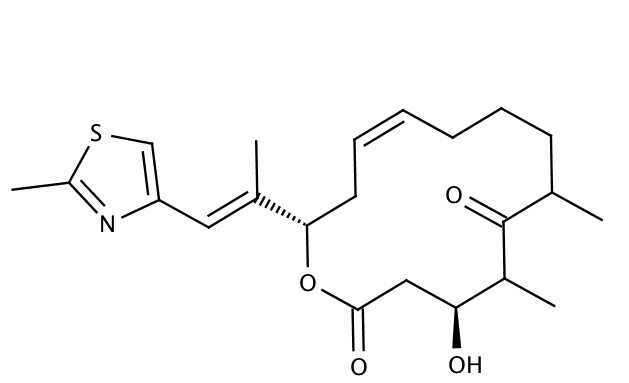
\includegraphics[width=4cm]{images/CID_23242270.png} & -9.24\\
     21 & 84 & 
     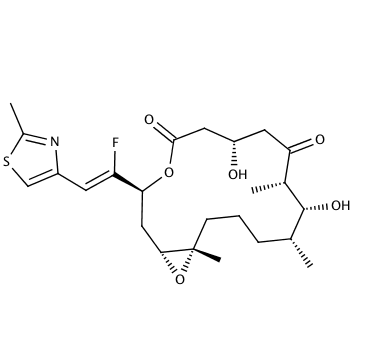
\includegraphics[width=3.7cm]{images/CID_20822803.png} & -9.08\\
     22\textsuperscript{\emph{c}} & 44 & 
     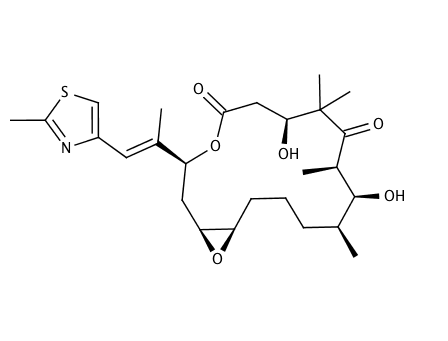
\includegraphics[width=4cm]{images/CID_448799.png} & -9.07\\
     23 & 118 & 
     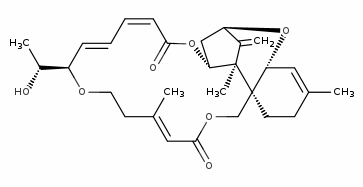
\includegraphics[width=4.5cm]{images/CID_10625150.png} & -9.06\\
     24 & 168 & 
     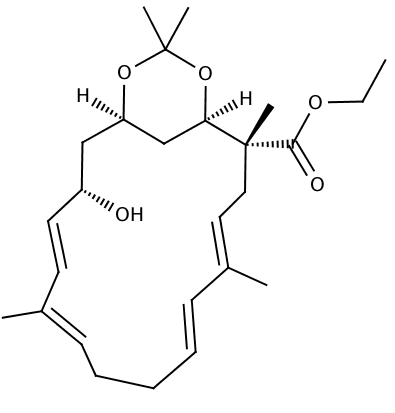
\includegraphics[width=2.7cm]{images/CID_10477941.png} & -9.03\\
    \bottomrule
  \end{tabular*} 
\vspace{-0.45cm}
   \begin{flushleft}
  \textsuperscript{\emph{a}} These are the IDs that we gave to the molecules;
  \textsuperscript{\emph{b}} Binding energy from AutoDock4.2 in kcal/mol;
  \textsuperscript{\emph{c}} The positive control, epothilone A.
  \end{flushleft}
\end{table}
Molecule 70 (CID 23242270) and 84 (CID 20822803) were not yet shown, experimentally, to have binding affinity toward tubulin. However, these three molecules have obvious similarity to the epothilone scaffold (molecule 44) and hence represent no new scaffold for us to adopt.
Molecule 118
(CID 10625150) is 12,13-deoxyroridin E which is produced by the marine-derived fungus \emph{Myrothecium roridum} and was shown by Namikoshi et al. to have cytotoxicity against human (HL-60) and murine (L1210) leukemia cell lines but until 2013 it has not yet been patented as an anticancer tubulin-binding agent
\cite{Namikoshi2001}.
This all shows that the protocol was strong enough in separating active from non-active molecules, with most of the strongly active molecules appearing on top of the list. The most attractive molecule is molecule 168 (CID 10477941) for it represents a completely new scaffold in this category of compounds. Not only is the scaffold entirely new, but its structure is much simpler than many tubulin binding
agents and appears to be very rigid. Due to its promising characteristics, we decided to undertake further optimization runs for this molecule through modification and redocking. 

As described in Sec.
\ref{ss:VS-Methods_Filtering}, 
we modified molecule 168 by addition of several functional groups to different positions in the molecule. The modification was based on visual inspection of the binding mode of molecule 168 to tubulin and on trying to optimize binding and the hydrogen bond network. We ran this modification/redocking step four consecutive times till the derivatives showed best affinity and no further improvements were obtained. 
\begin{figure}
  \centering
  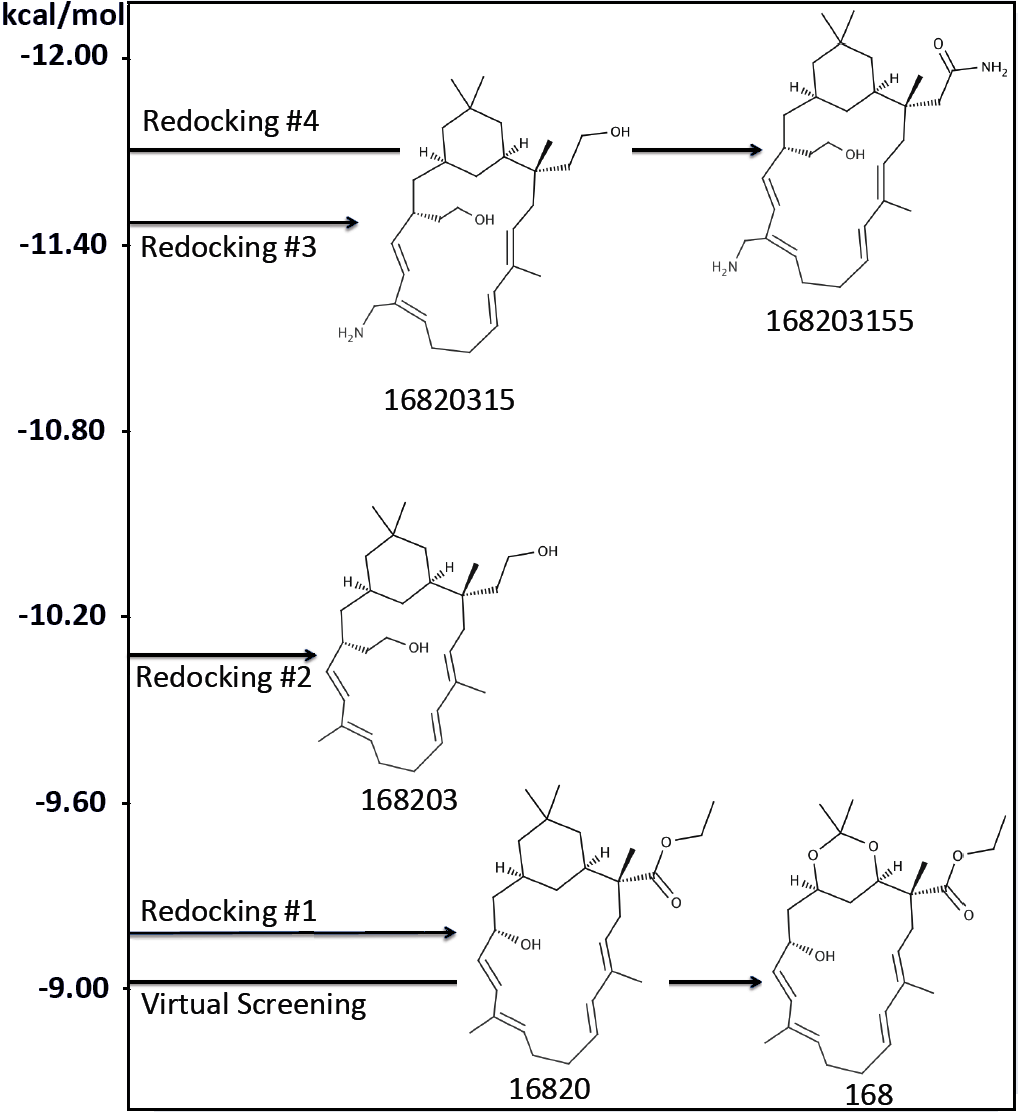
\includegraphics[width=0.6\linewidth]{images/Redock4.png}
  \caption[Quantitative improvement of binding energies]{Quantitative improvement of binding energies (on the y-axis) of the top hits obtained in each of the consecutive modification/redocking runs on molecule 168.}
  \label{f:VS-Redock}
\end{figure}
Fig. \ref{f:VS-Redock} shows the top hits from each run and shows the trend of the improvement of the binding affinity following our modification/redocking protocol. 
It is clear that this protocol managed to bring molecule 168 
from a binding affinity of $-9.03$ kcal/mol to a binding affinity of
$-11.76$ kcal/mol (molecule 168203155) which is much higher than the top hit obtained in the first virtual screening run (molecule
38 with a binding energy of $-10.03$ kcal/mol). However, these hits that we obtained appear to be highly lipophilic and their water solubility, and absorption could be questioned.
These are serious drawbacks in the context of chemotherapy applications. Therefore, we decided to run another modification/redocking run on the best hit, molecule 168203155, with the purpose of only increasing the hydrophilicity of the derivatives, while still maintaining a good affinity.

Table
\ref{t:VS-fifthRun} shows the result of this fifth run with the corresponding binding energies of each derivative. It shows that we could not get any derivative to be any better than the parent molecule, molecule 168203155, in terms of binding energy. However, their binding energies are still in the top range and we managed to increase their hydrophilicity by the inclusion of hydrophilic functional groups. It is worth mentioning that all the derivatives of molecule 168 are very rigid and there is only one mode of binding available for these molecules in the tubulin binding site. Within an RMSD of 2.00 \r{A}, nearly all the binding poses would group in one cluster. This rigidity can be exploited in tailor designing analogs that are more selective toward certain tubulin isoforms over the others, thus increasing the specificity of the treatment.

\begin{table}
  \caption[Binding energies in the fifth modification/redocking run]{Binding energies in the fifth modification/redocking run of the derivatives of molecule 168203155.}
  \label{t:VS-fifthRun} 
  \centering 
  \begin{tabular*}{\linewidth}{@{\extracolsep{\fill}}>{\centering\arraybackslash}m{1cm}>{\centering\arraybackslash}m{2cm}>{\centering\arraybackslash}m{2.7cm}>{\centering\arraybackslash}m{1.2cm}}
    \toprule
    Rank & ID  &  
    Molecule & $\Delta{E}$ \textsuperscript{\emph{a}}\\
    \midrule
    \\
    1 & 1682031551 & 
     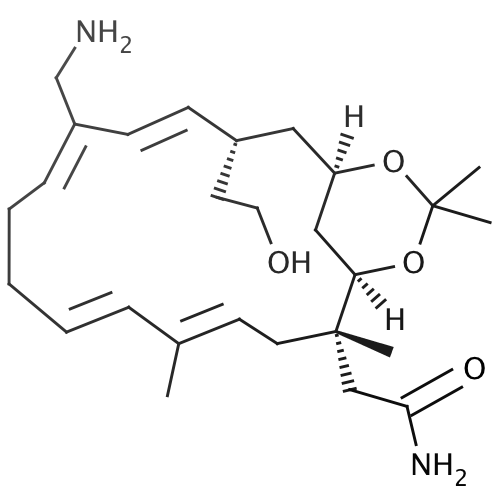
\includegraphics[width=2.6cm]{images/1682031551.png} & -11.47\\
     2 & 1682031559 & 
     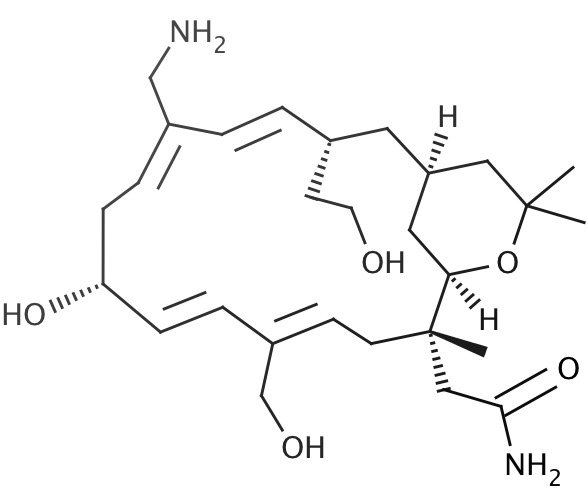
\includegraphics[width=2.7cm]{images/1682031559.png} & -11.22\\
     3 & 1682031553 & 
     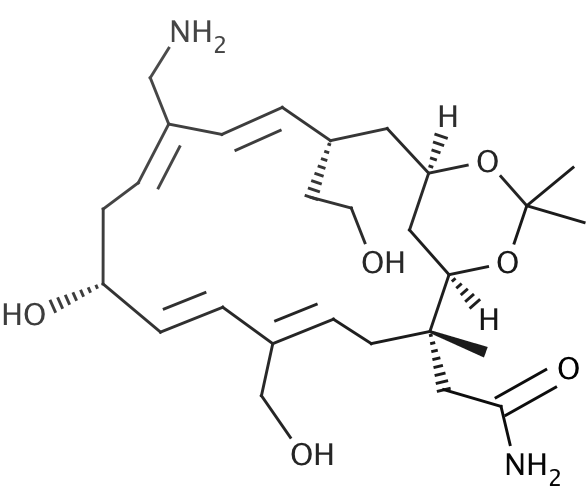
\includegraphics[width=2.7cm]{images/1682031553.png} & -11.06\\
     \bottomrule
  \end{tabular*}
  \vspace{-0.45cm}
     \begin{flushleft}
  \textsuperscript{\emph{a}} Binding energy calculated by AutoDock 4.2 in kcal/mol.
  \end{flushleft}
\end{table}

Fig. \ref{f:VS-Binding}(a) 
shows the binding of molecule 1682031551 to 
$\beta$-tubulin where the ligand forms five hydrogen bonds with Thr274, Arg282, Arg318, Asp26 and Ala231. Such a strong network of hydrogen bonds should help fixing the ligand in position and enhancing its affinity. This could be compared to the hydrogen bond network of epothilone A in $\beta$-tubulin, Fig.  \ref{f:VS-Binding}(b), 
where residues Thr274, Arg276, His227 and Arg282 form hydrogen bonds with the ligand as also pointed out by Nettles et al.
\cite{Nettles2004}. 
Thr274 and Arg282 are residues in common for the two ligands, but Asp26, Arg318 and Ala231 are specific to our new molecule. This could foretell that the molecule might be effective in epothilone-resistant cell lines.

\begin{figure}
\centering
\subfloat[molecule 1682031551]{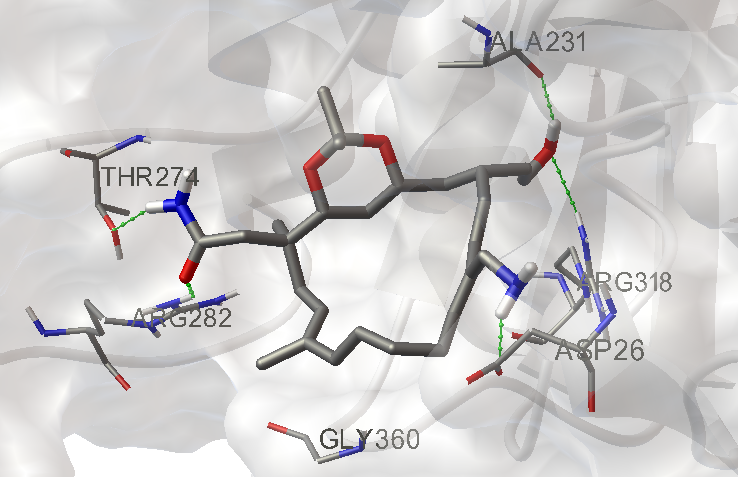
\includegraphics[width=0.48\linewidth]{images/1com2.png}}
\hspace{0.1cm}
\subfloat[Epothilone]{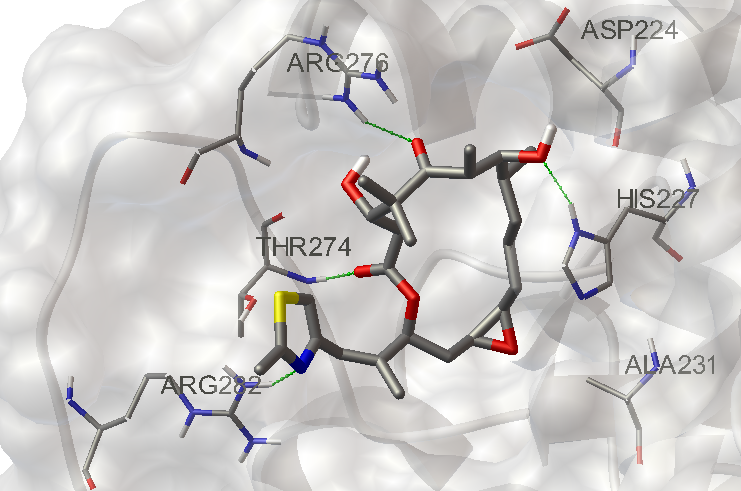
\includegraphics[width=0.48\linewidth]{images/epocom3.png}}
\caption{Ligand poses in taxol
binding site.}
\label{f:VS-Binding}
\end{figure}

\subsection{Results of Rescoring via MM/PBSA}
\label{ss:VS-Results_Rescoring}

Molecular dynamics simulations were run for the all complexes
(five test molecules and three highest-scoring hits). The five test molecules, discodermolide, eleutherobin, epothilone A, paclitaxel and sarcodictyin A, were used as a test for the predictive power of
the method. Before using the MM/PBSA script, the five complexes were checked for equilibration of total energy, temperature, density and RMSD and we made sure that they were well-equilibrated. Fig.
\ref{f:VS-rmsd}a 
shows the RMSD equilibration for the five complexes, each of which was equilibrated for at least the last 5 ns of the simulation which was then post-processed using MM/PBSA for binding energy calculation. Enthalpic contribution was calculated using the last 500 evenly spaced snapshots extracted from the last 5 ns. This ensures that each two consecutive snapshots are 10 ps apart and hence uncorrelated. The entropic contribution was calculated using normal mode analysis with 48 evenly spaced snapshots also extracted from the last 5 ns. We could not use more snapshots because normal mode analysis is highly demanding in terms of
computational power. The experimental binding constants, $K_b$, of the five test molecules to the taxol binding site were determined by Buey et al. through displacement of the fluorescent taxoid Flutax-2
\cite{Buey2004,Buey2005}. These values are presented in 
Table \ref{t:VS-deltaG}, together with the binding free energies,
$\Delta{G}^{o}$, calculated from the binding constants via the following thermodynamic relationship:
\begin{equation}
\label{eq:VS-dG/K}
\Delta{G}^{o} = -RT \ln K_{b}
\end{equation}
where R is the universal gas constant, $R$ = 1.987 cal mol$^{-1}$K$^{−1}$, and $T$ is the absolute temperature. The experimentally derived binding energy, $\Delta{G}^{o}$, for each molecule was plotted against the MM/PBSA 
predicted value as shown in Fig.
\ref{f:VS-regression}. 
\begin{figure}
\centering
\subfloat[]{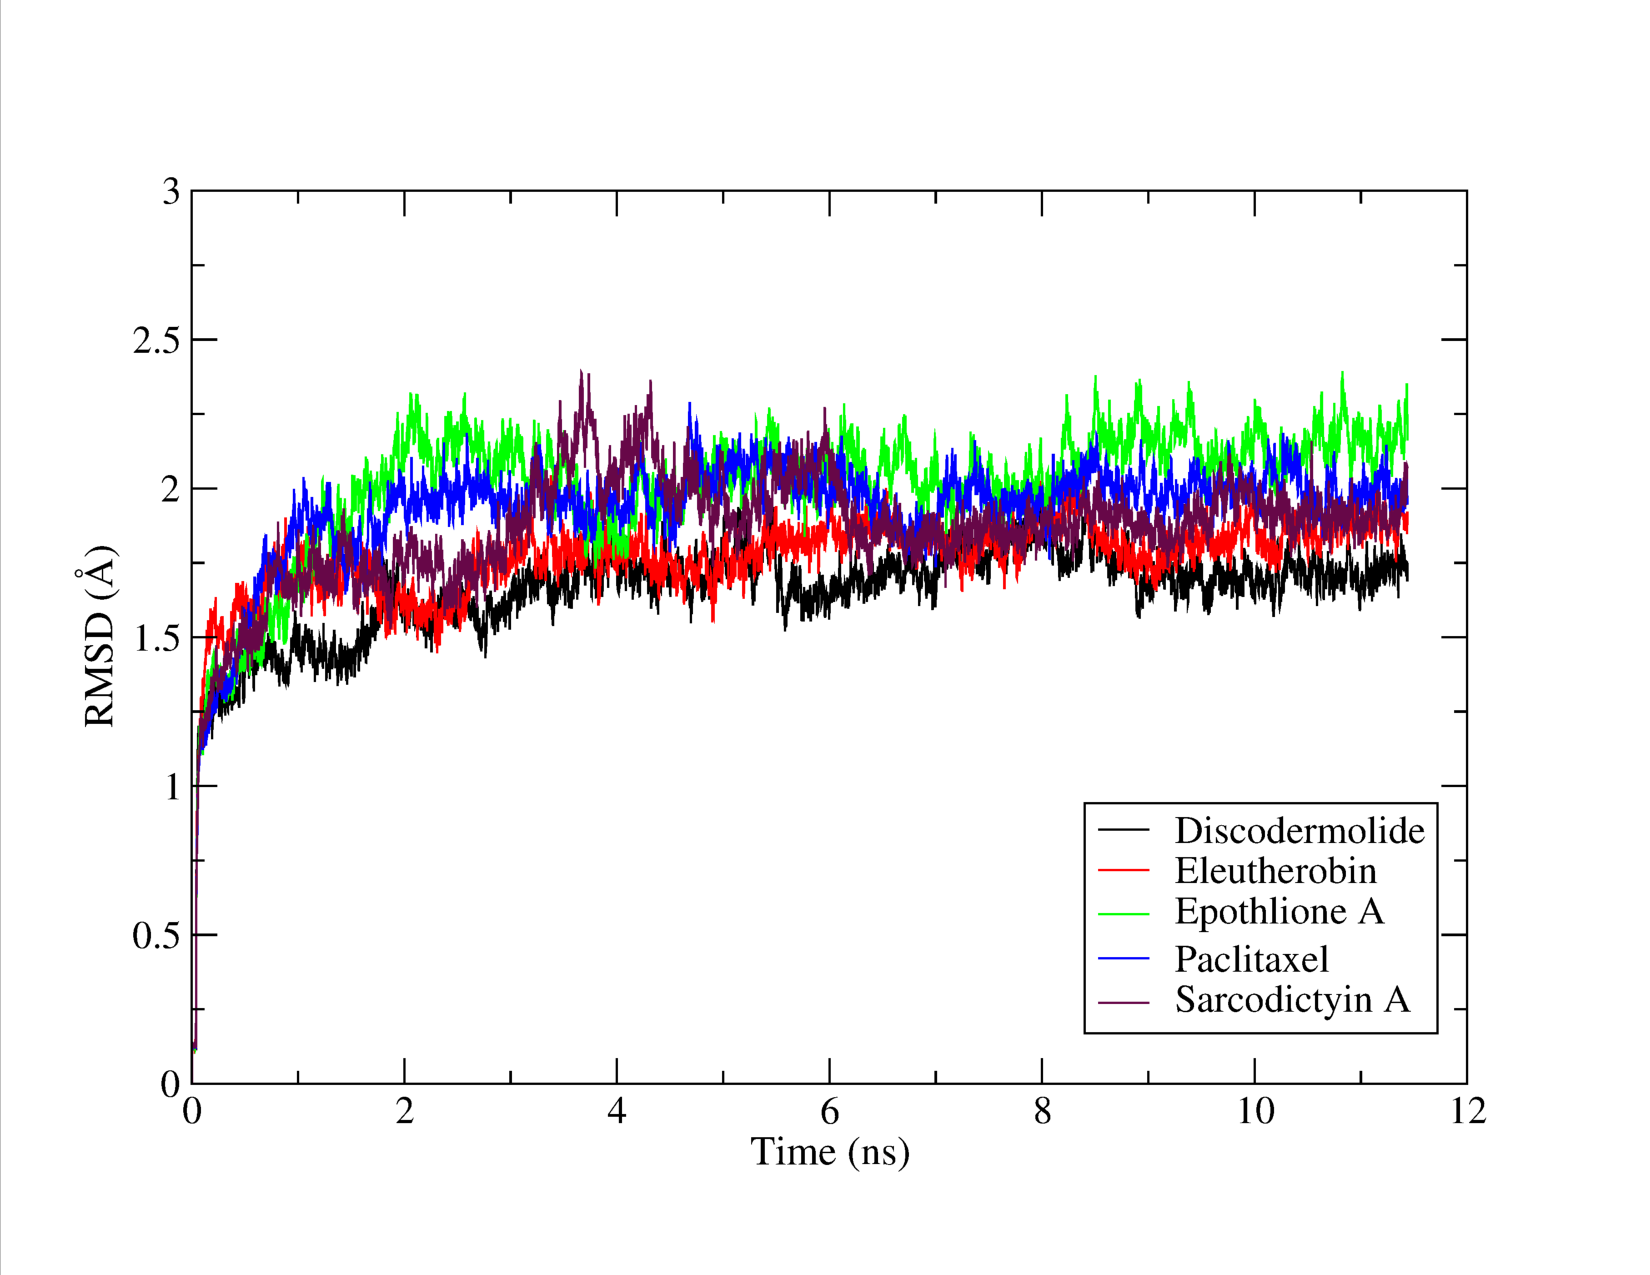
\includegraphics[trim=1.2cm 1.7cm 2cm 2.7cm, clip=true, width=0.49\linewidth]{images/8-13_rmsd}}
\subfloat[]{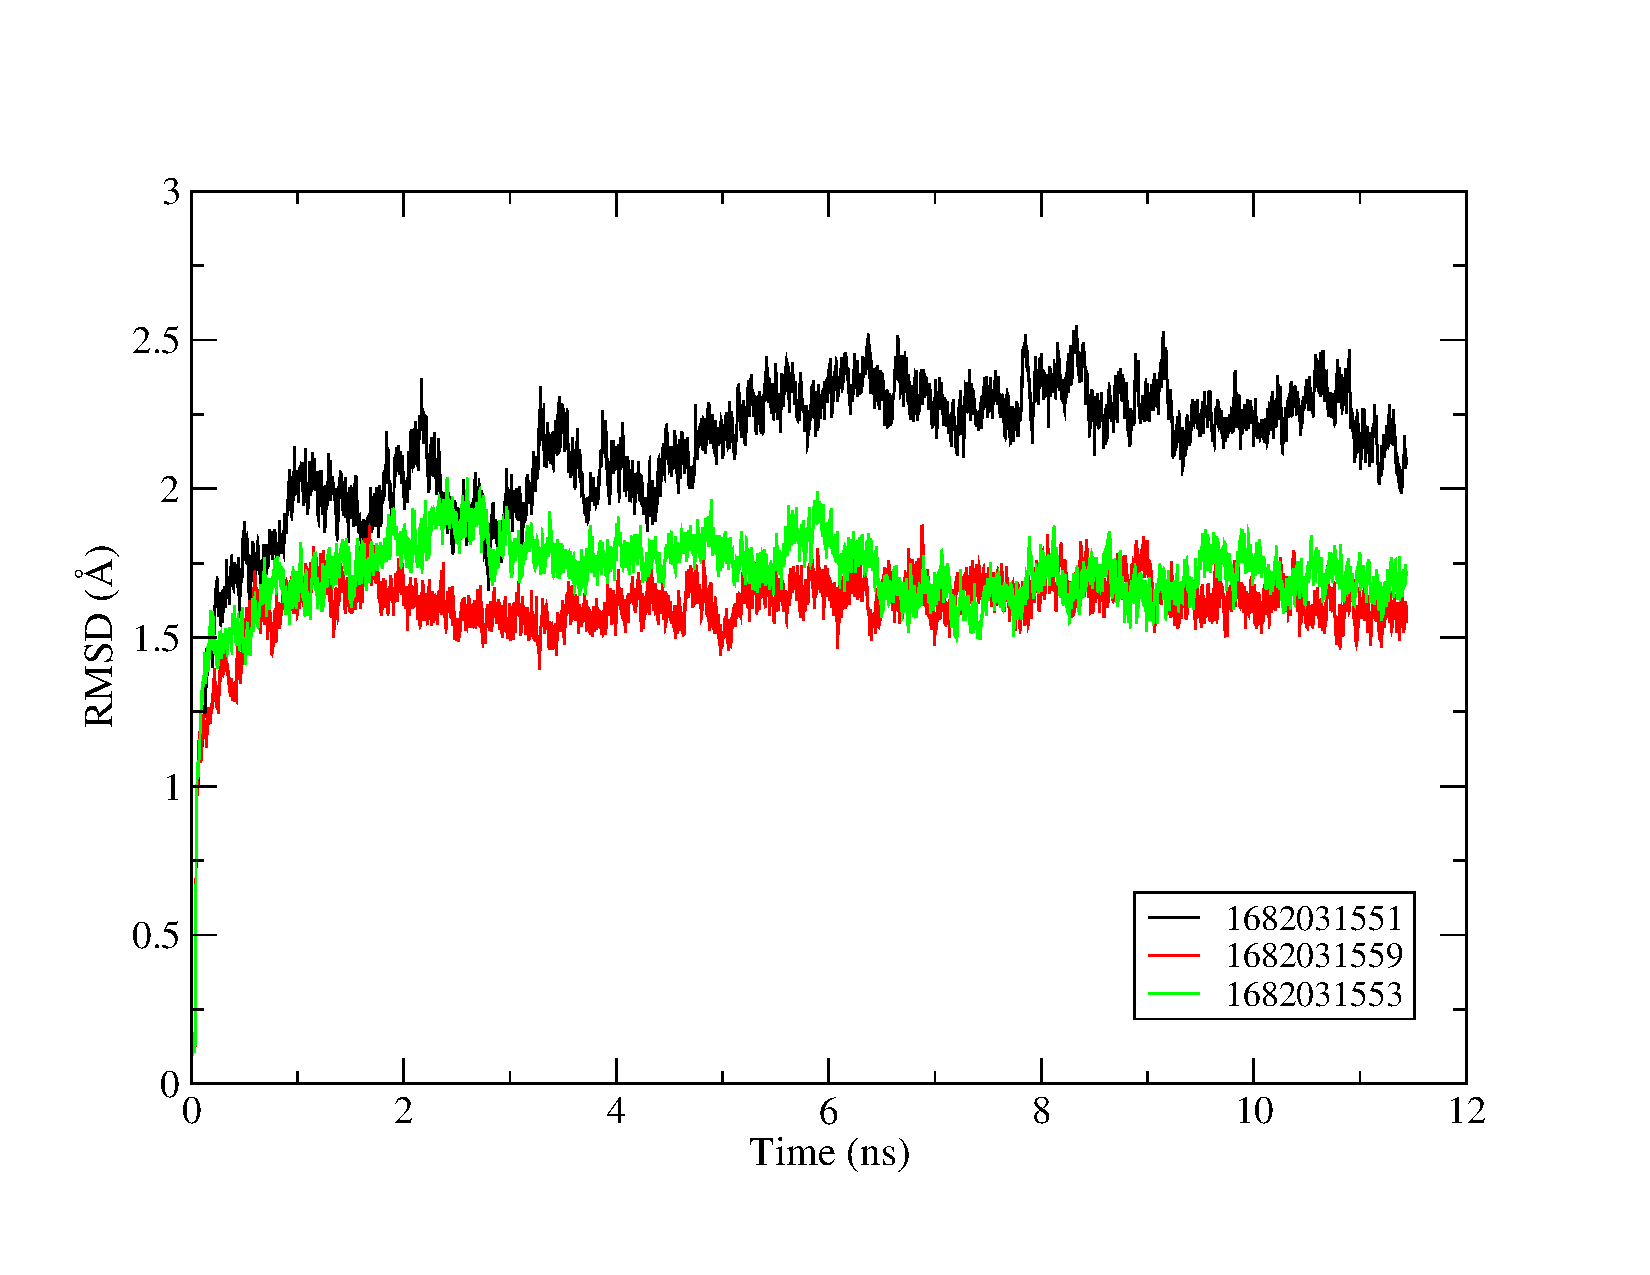
\includegraphics[trim=1.2cm 1.7cm 2cm 2.7cm, clip=true, width=0.49\linewidth]{images/246_rmsd}}
\caption[RMSD equilibration]{RMSD equilibration
of the ligand-receptor complexes of the five ligands with experimental data (a)
and of our three novel hits (b).}
\label{f:VS-rmsd}
\end{figure}
The figure shows the linear fit of the data which produces an excellent linear correlation with a coefficient of determination, $R^{2}$, of 0.99, a slope of 0.2 and an
intercept of $-4.6$ kcal/mol.
This proves that the MM/PBSA protocol that we followed here
is a reliable method in predicting the binding energies of the tubulin ligands binding at the taxol binding site and hence can be
carried forward and used to predict the binding energies of the novel hits that we obtained from the screening protocol. Thus, the same MM/PBSA protocol was applied for the three highest-scoring hits shown previously in 
Table \ref{t:VS-fifthRun} , namely molecules 1682031551, 1682031559 and 1682031553. As was done previously with the test molecules, we checked the complexes of these three ligands for equilibration of the total energy, temperature, density and RMSD and made sure that they were all well-equilibrated.

\begin{table}[h]
  \centering
  \caption[Experimental binding constants]{Experimental binding constants, $K_{b}$, of the five test molecules and the 
  corresponding values of the binding free energies, $\Delta{G}^{o}$.}
  \label{t:VS-deltaG}
  \begin{tabular*}{\linewidth}{@{\extracolsep{\fill}}lcc}
   \toprule
   Ligand & $K_{b}$ ($10^{7} M^{-1}$)\textsuperscript{\emph{a}} & $\Delta{G}^{o}$ (kcal/mol)\textsuperscript{\emph{a}} \\
   \midrule
   Discodermolide & 837 $\pm$ 77 & -13.6 $\pm$ 0.1 \\
   Eleutherobin & 3.26 $\pm$ 0.25 & -10.3 $\pm$ 0.05 \\
   Epothilone A & 6.94 $\pm$ 1.08 & -10.8 $\pm$ 0.1 \\
   Paclitaxel & 2.19 $\pm$ 0.05 & -10.1 $\pm$ 0.01 \\
   Sarcodictyin A & 0.23 $\pm$ 0.09 & -8.7 $\pm$ 0.2 \\
   \bottomrule
  \end{tabular*}
  \vspace{-0.45cm}
     \begin{flushleft}
  \textsuperscript{\emph{a}} Data $\pm$ standard error; average of at least four 
   independent measurements \cite{Buey2004,Buey2005}.
   \end{flushleft}
\end{table}
Fig. \ref{f:VS-rmsd}b 
shows the equilibration of RMSD of the three complexes and confirms that the three complexes were equilibrated at least in the last 5 ns. We then post-processed these 5 ns in the same way as the previous complexes and used 500 evenly spaced snapshots for enthalpy calculation and 48 evenly-spaced ones for normal mode analysis.
\begin{figure}
\centering
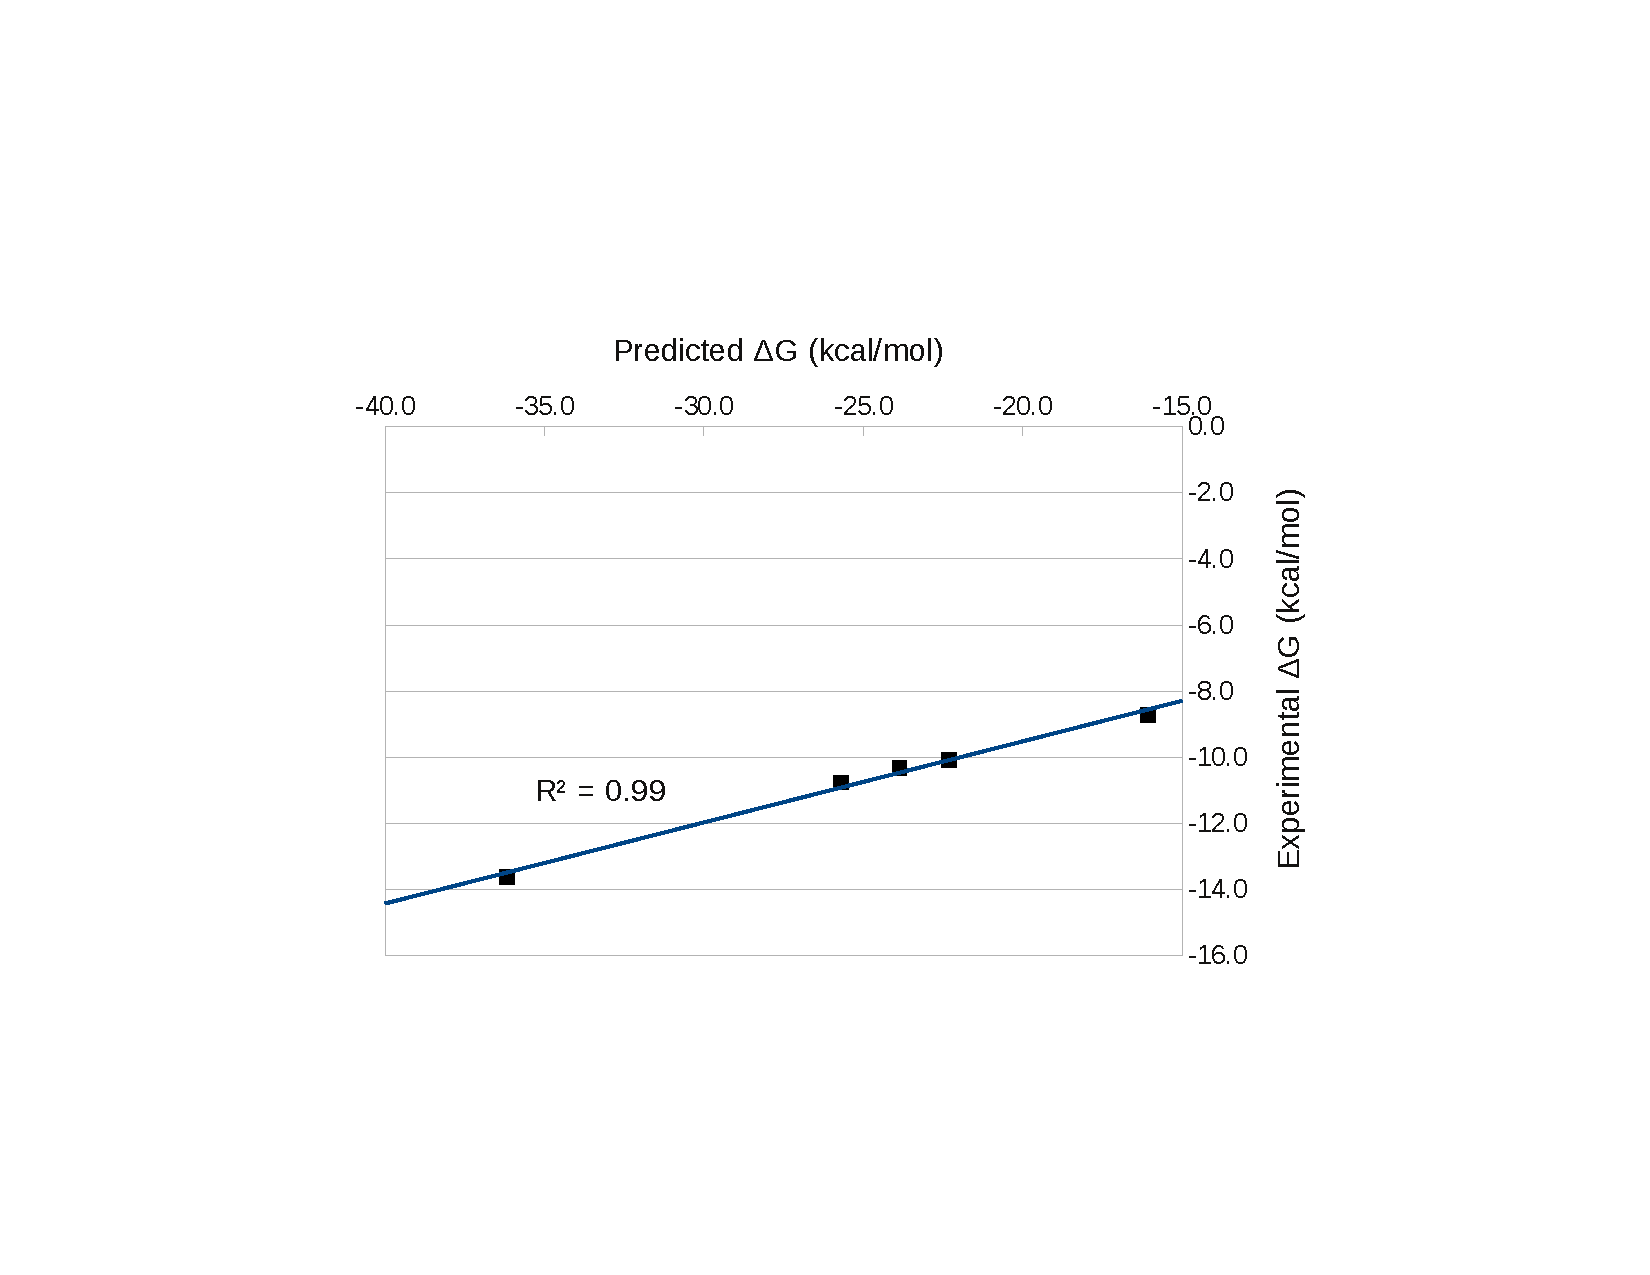
\includegraphics[trim=6cm 5cm 5cm 5cm, clip=true, width=0.7\linewidth]{images/Regression_plot}
\caption[Linear regression plot]{linear regression plot of the MM/PBSA-predicted binding energies versus the experimentally derived values.}
\label{f:VS-regression}
\end{figure}
The results of this prediction, after extrapolation through the linear fit presented 
Fig. \ref{f:VS-regression}, are shown in 
Table \ref{t:VS-hitdG}. 
The results in the table clearly confirm the outcome of the docking experiments and predict that the novel hits may have strong binding energies to the taxol binding site. Molecule 1682031551 shows the lowest predicted binding free energy, $-14.7$ 
kcal/mol, which is much lower than all of the test molecules shown in 
Table \ref{t:VS-deltaG}, all of them being strong tubulin stabilizers. 
Molecule 1682031553 is also predicted to have a strong affinity of $-12.5$ kcal/mol toward the taxol binding site which surpasses all of the test molecules except for discodermolide. Finally, molecule 1682031559 is predicted to have an affinity of $-10.8$ kcal/mol which is still better than paclitaxel,
eleutherobin and Sarcodictyin A. In general, these results meet the aim of the study, confirm our findings in the docking runs and show that our novel scaffold could act as a good anticancer tubulin-binding agent.
\begin{table}[h]
  \centering
  \caption[Extrapolated binding energies of novel hits]{Extrapolated binding energies of novel hits as predicted by the
  MM/PBSA protocol.}
  \label{t:VS-hitdG}
  \begin{tabular}{p{0.3\linewidth}p{0.3\linewidth}}
   \toprule
   Ligand & $\Delta{G}$ (kcal/mol)\textsuperscript{\emph{a}} \\
   \midrule
   1682031551 & -14.7 $\pm$ 0.9 \\
   1682031559 & -10.8 $\pm$ 0.6 \\
   1682031553 & -12.5 $\pm$ 0.7 \\
   \bottomrule
  \end{tabular}
  
  \textsuperscript{\emph{a}} Extrapolated value $\pm$ standard error based
  on a 95\% confidence interval.
\end{table}

\subsection{Results of Physicochemical Predictions}

After predicting that our new molecules should have high affinity toward the taxol binding site, we checked the physicochemical and toxicological properties of them and compared them to known \glspl{MSA} to see how our now candidates will compare in terms of drug pharmacokinetics. Table \ref{t:VS-AMDE}
shows the different parameters calculated by ADMET Predictor software. The partition coefficient (log $P$) is a measure of lipophilicity. It shows that our molecules span a wide range of lipophilicity from 5.33 to 0.94. This is useful since lipophilicity is required for some drugs acting on the brain so that they can pass through the blood-brain barrier which may help with brain tumors. However, too lipophilic compounds might not be soluble in the intestinal fluids and less lipophilic compounds are preferred in this case. The distribution coefficient (log $D$) is different from log $P$ for all our four new compounds which shows that they are all ionizable. The effective human jejunal permeability ($P_{\emph{eff}}$) decreases with decreasing lipophilicity and spans a wide range from 1.35 to 0.14 $\mu$m/s. Interestingly, the solubility in simulated intestinal fluid in fasted state (FaSSIF) is much higher for our new compounds when compared to epothilone A. The solubility of compound 1682031553, for example, is almost 100-fold better than epothilone A, our positive control. Achieving molecules with better solubility was one of the main aims of the study since paclitaxel,
for example, is insoluble in water and this was one of its drawbacks
\cite{Singla2002}. Therefore, the physicochemical profiles of our molecules do achieve one of the aims of this study, that is; finding new tubulin binding candidates with better pharmacokinetic profiles. As to the predicted toxicity of these compounds, all of them showed potential hepatotoxicity, with 1682031559 and 1682031553 showing potential SGOT and SGPT enzyme elevation. Only compound 168203155 showed potential acute rat toxicity. We compared this profile to the predicted profile of our positive control, epothilone A, which showed potential hepatotoxicity and carcinogenicity in rats. Therefore, the toxicological profiles of our molecules and epothilone A are not identical and when carcinogenicity is considered, our molecules may do better than epothilone A as they are predicted to be devoid of this toxic side effect. However, all these are data predicted from simulations, and toxicological assays will indeed be needed to confirm such findings.
\begin{table}
\centering
  \caption[Predicted physicochemical properties of the novel hits]{Predicted physicochemical properties of the novel hits compared
  to epothilone A}
  \label{t:VS-AMDE}  
  \begin{tabular*}{\linewidth}{@{\extracolsep{\fill}}llrcc}
    \toprule
    Ligand & log P  & log D & \shortstack{$P_\emph{{eff}}$ ($\mu$m/s)} & FaSSIF (mg/mL)\\
    \midrule
    168203155\textsuperscript{\emph{a}} & 5.33 & 3.52 & 1.35 & 0.0615\\
    1682031551 & 3.21 & 1.55 & 0.47 & 0.501\\
    1682031559 & 1.81 & 0.35 & 0.28 & 1.89\\
    1682031553 & 0.94 & -0.45 & 0.14 & 3.99\\
    Epothilone A & 3.07 & 3.07 & 1.46 & 0.0433\\
    \bottomrule
  \end{tabular*}
   \vspace{-0.45cm}
   \begin{flushleft}
\textsuperscript{\emph{a}} The parent compound of the fifth run. It is listed here to show how the fifth 
run affected the lipophilicity of the compounds. See Table \ref{t:VS-fifthRun}.
   \end{flushleft}
  \end{table}
  
\section{Conclusion}
\label{s:VS-Conclusion}

The similarity-based virtual screening study reported here
predicted five active molecules that have not been patented as tubulin-binding agents before. One of them, molecule 168, is very promising and possesses a novel scaffold. Upon modifying this molecule, optimizing its binding to the receptor and redocking its derivatives in subsequent runs, we managed to obtain several derivatives that are superior to the parent compound, molecule 168, in terms of calculated binding affinity to the target and physicochemical properties. They also showed superiority in binding energy over known tubulin binding agents. Rescoring of the top hits using the MM/PBSA protocol confirmed our findings and showed that at least three of our top hits possess higher binding affinities than the five tubulin stabilizers that were used as query molecules in the similarity-based filtration step. The predicted physicochemical properties of the new compounds also show superiority to the known tubulin stabilizers especially regarding solubility in the intestinal fluid. The toxicological profile predicts comparable toxicity to known MSAs except for carcinogenicity which our new molecules were devoid of. As a follow-up to this study, the next step should be synthesizing these molecules and testing their activities experimentally to confirm the computational findings. It is hope that this work will lead to the development of new and improved cancer chemotherapy compounds.

\bigskip 

\chapter{Unravelling the Mechanism of Action of Antitumor Lankacidin}
\label{lankacidin}

\section{Summary}

Lankacidin group antibiotics are known to have antitumor activities with unclear
mechanism of action. Based on a previous virtual screening study for
taxol-like drugs which
produced hits very close in structure to lankacidin, we suggest
that the cytotoxic effect of lankacidin antibiotics is due to microtubule
stabilization though a taxol-like mechanism. This suggestion was confirmed
both computationally using molecular dynamics simulations and binding energy calculations and experimentally using fluorescence quenching assays.

\section{Introduction}

Lankacidin-group antibiotics (T-2636) are fermentation products that are produced by the
organism \emph{Streptomyces rochei}
\cite{Harada1969}. First isolated in 1969, the antibiotic
group was later
fully characterized and the structure of lankacidin was
elucidated \cite{Harada1971,Harada1973,Harada1973b,Harada1974}.
The parent of this group, lankacidin C Fig. \ref{f:Lank-truc}a, is a 17-membered macrocyclic tetraene which shows
strong antimicrobial activity against various Gram-positive
bacteria, including many strains that are resistant to 
macrolide antibiotics, and 
is used in veterinary medicine \cite{Tsuchiya1971}. 

Besides its
antimicrobial activity, lankacidin C and
some of its derivatives
also displayed considerable \emph{in vivo} antitumor
activity against L1210 leukemia, B16 melanoma and
6C3 HED/OG lymphosarcoma \cite{Ootsu1973,Ootsu1975}.
In addition to these pharmacological activities, being well-tolerated \emph{in vivo}, 
displaying low toxicities in mice
\cite{Harada1973b} and having a complete synthetic 
pathway available \cite{Kende1995} makes the molecule very attractive for drug research.

The antimicrobial mechanism of action
of lankacidin has been attributed to interference with
peptide bond formation during
protein synthesis by binding at the peptidyl transferase center of the eubacterial large ribosomal subunit
\cite{Auerbach2010,Belousoff2011}.
It is unclear, however, whether the antitumor
activity of lankacidins is related to their interference
with protein synthesis or not \cite{Ootsu1975}.
Hence, the mechanism of antitumor activity of lankacidins
is yet to be elucidated. 

In a previous virtual screening
study for taxol-like microtubule stabilizers, we
have identified a novel scaffold predicted to bind 
to tubulin at the taxol binding site \cite{Ayoub2013}.
Due to difficulties synthesizing this novel 
compound, we tried to search for available molecular
structures that resemble it. It turned out that the
molecular framework of our novel
hit very closely resembles that of lankacidin \cite{Ayoub2013}.
The striking similarity between the two compounds
suggests a hypothesis that lankacidin C could 
also bind to tubulin at the taxol binding site
which could explain its unknown 
antitumor mechanism of action. 
In addition to explaining their mechanism of
action, if this hypothesis
is tested and proven true, this would widen our understanding
of microtubule stabilization by taxol-like agents and 
would also open the door for structural modifications of the low-toxicity synthetically-available lankacidins
towards better binding with tubulin. This may help provide
a promising cancer treatment. On the computational side,
if the hypothesis is proven, this would provide a good
example of the power of computational predictions 
and their aid in explaining chemical and pharmacological
processes.

\begin{figure}
\centering
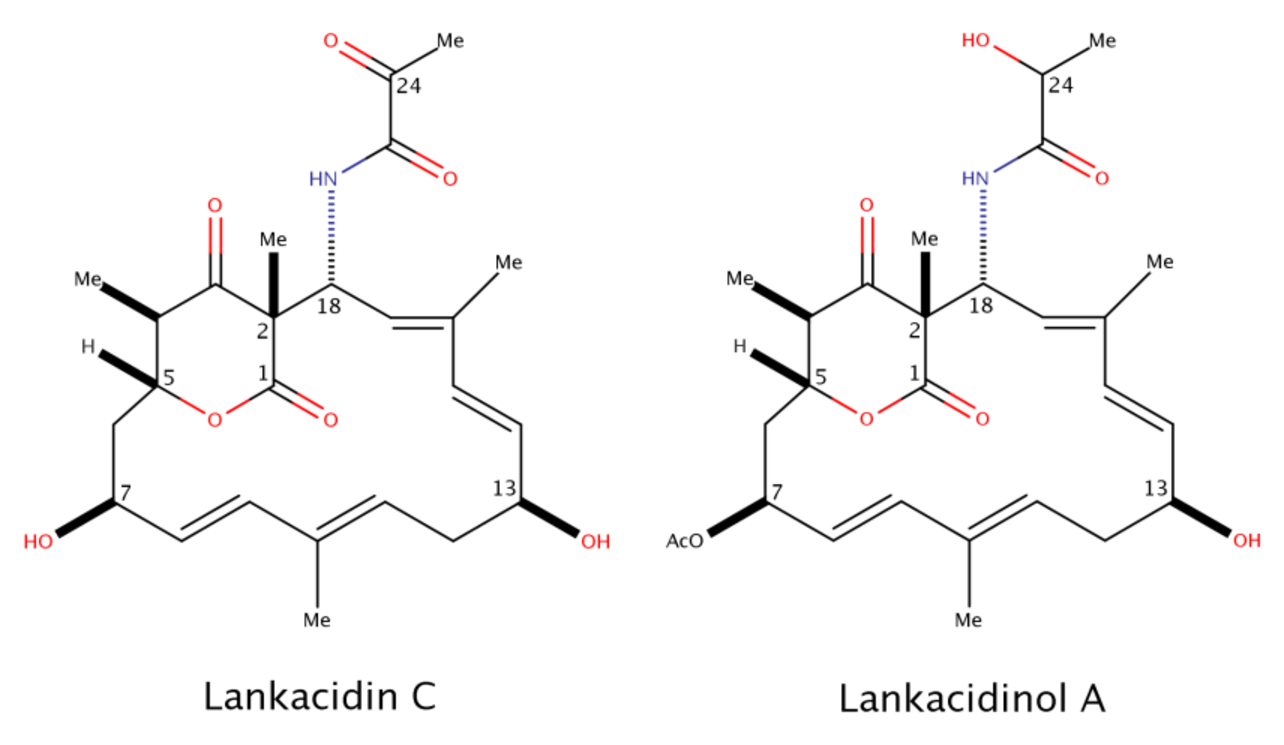
\includegraphics[width=0.98\linewidth]{images/LankStruc.pdf}
\caption[Structure of lankacidin C and lankacidinol A]{Structure of lankacidin C and lankacidinol A}
\label{f:Lank-truc}
\end{figure}


\section{Methodology}

\subsection{Computational Simulations}
Computational simulations of lankacidin C
bound to the taxol binding site in $\beta$-tubulin
were carried out according to the procedures outlined
in previous work \cite{Ayoub2013}. 
Briefly, we parameterized GDP-bound $\beta$-tubulin
subunit using AMBERff99SB forcefield for the protein
\cite{Hornak2006}
and Meagher et al. parameter set for GDP molecule
\cite{Meagher2003}.
Lanakcidin C was parameterized using the GAFF force field \cite{Wang2004}.
Prior to molecular dynamics simulations, the crystal structure
of lankacidin C from \gls{pdb} ID:3JQ4
was docked to the taxol binding site using AutoDock 4.2
as explained in \cite{Ayoub2013}. The complex was then 
neutralized, solvated, heated to 300K, and taken through a molecular dynamics
simulation for density equilibration followed by a production phase for
nearly 11 ns using the Amber package \cite{case2012}. Evenly-spaced
snapshots from the last 5 ns of the simulation were used for
an MM/PBSA binding energy calculation in which 
both the enthalpy (500 snapshots) and entropy (48 snapshots) were estimated, the latter using
normal mode analysis. Using the linear fitting that was developed
in \cite{Ayoub2013}, we extrapolated the MM/PBSA-calculated binding energy
to get a more realistic value that could be compared to binding energies 
of available 
microtubule stabilizers.

\subsection{Isolation of Lankacidin} \emph{Streptomyces rochei} strain 51252 \cite{Kinashi1994} was cultured in YM liquid medium 
(0.4\% yeast extract, 1.0\% malt extract, and 0.4\% D-glucose, pH 7.3) at 28$\celsius$
for 2 days. 
The culture broth was extracted twice with equal volume of ethyl acetate. 
The combined organic phase was dried (Na$_{2}$SO$_{4}$), filtered, and 
concentrated to dryness. The crude residue was purified by Sephadex LH20 
(GE Healthcare) with methanol. The fractions containing lankacidin C and 
lankacidinol A were combined, and further purified by silica gel chromatography 
with a mixture of chloroform-methanol (50:1-20:1). All the spectral data for 
lankacidin C and lankacidinol A were identical to the reported data \cite{Arakawa2005} \footnote{Isolation of lankacidin was carried out by 
K. Arakawa, Hiroshima University, Japan.}.

\subsection{Fluorescence Quenching Assays}
Reagents were purchased from Sigma-Aldrich Canada Ltd. (Oakville, Ontario, Canada) and Fisher Scientific Company (Ottawa, Ontario, Canada).
In a 96-well microplate, equimolar mixtures of recombinant human tubulin TUB-BI or porcine cytoskeleton tubulin protein 
(purchased from Cytoskeleton Inc; Cat. \# T240-DX)
and the buffer (10 mM sodium phosphate, 10 mM MgCl$_{2},$ 1 mM guanosine 5'-tri-phosphate (GTP), 0.5\% DMSO, 250 mM sucrose, pH = 7.0) were mixed to reach a final tubulin (dimer) concentration of 2 $\mu$M. GTP was added to the samples to a final concentration of 1 mM. The microplate was incubated on ice for 10 min to allow for the formation of the tubulin dimer. The calculated amounts of stock solution of the compounds in DMSO were added to the protein samples to obtain final ligand concentrations of 5, 10, 20, 40, 60, 80 and 100 $\mu$M. The control was ligand-free, and the total sample volume was 100 $\mu$L. A glass bead was inserted into each well, and the microplate was covered with a protective
film, sealed with a lid, and incubated for 30 min at 25$\celsius$. After that time, the microplate was transferred to a rotating platform and vigorously rotated for 1 h at room temperature. From each well, 80 $\mu$L of samples and control was transferred to a 1-cm fluorescence cell. Fluorescence spectra were collected on a PTI MODEL-MP1 spectrofluorometer using 10 mm path length cell at 295 nm (excitation wavelength), and the scan range was 310--400 nm. Spectral data were collected using fluorescence software, and data analysis was performed using ORIGIN 6.1 software (OriginLab, Northampton, MA).

\subsection{Determination of Kinetic Parameters}
Data from the fluorescence experiments were used to determine the apparent binding constant of ligands to tubulin dimers by using the Stern--Volmer equation:
\begin{equation}
\label{eq:stern-volmer}
\dfrac{F_0-F}{F}=K_a[L]
\end{equation}
here $F_0$ and $F$ are the fluorescence intensities in the absence and in the presence of quencher, respectively, $K_a$ is the formation constant of the donor--acceptor (quencher--fluorogen) complex, and $[L]$ is the concentration of the ligand added. Excitation and emission slits were set at 4 nm. All spectra were collected with samples having final optical densities (1 cm) $<$ 0.3 at maximum absorbance of added ligand and were corrected for the inner filter effect according to the following equation:
\begin{equation}
\label{eq:correction}
F_{\text{corr}} = 10^{(A_{ex} + A_{em})/2} F_{\text{obs}}
\end{equation} 
where $F_{\text{corr}}$ is the corrected fluorescence, $F_{\text{obs}}$ is the measured fluorescence, $A_{ex}$ is the absorption value at the excitation wavelength (295 nm), and $A_{em}$ is the absorption value at the emission wavelength (336 nm). From the slope of the linear plot of $({F_0-F}/{F})$ versus $[L]$, binding constant values were estimated. The results are expressed as mean values $\pm$ \gls{sd} (n=4). \footnote{Fluorescence quenching experiments were
carried out by R. Ahmed, Department of Biochemistry, University of Alberta.}


\section{Results}

\subsection{Computational Predictions}

The equilibrated trajectory of the complex of
lankacidin C and $\beta$-tubulin was post-processed by removal of
water and ions from the last 5 ns and a MM/PBSA and normal mode analysis 
were run. The MM/PBSA returned a binding enthalpy of 
$-34.5$ kcal/mol while the normal mode analysis returned an
entropic contribution ($T\Delta S$) of $-23.4$ kcal/mol. Both
values yield a calculated binding free energy of $-11.1$ kcal/mol.
Utilizing the linear fitting that was developed in previous
work \cite{Ayoub2013}, this value can be extrapolated using the 
following relationship
\begin{equation}
\Delta G_\text{predicted} = 0.2\,\,\Delta G_\text{calculated} - 4.7
\end{equation}
to give the predicted binding energy of lankacidin C to 
the taxol binding site. The equation yields a predicted
binding energy of $-7.4\pm0.9$ kcal/mol. When this value
is compared to known taxol-like microtubule stabilizers upon which the linear fit was built, it is closest to sarcodityin A which has a predicted
binding energy of $-8.55\pm0.7$ kcal/mol \cite{Ayoub2013}. Since it is 
established in previous studies that the antitumor activity of 
lankacidin C is relatively weak \cite{Ootsu1973,Ootsu1975},
the comparison of our predicted binding energy of lankacidin C
to the taxol binding site versus that of sarcodictyin A
seems plausible. Based on our predicted binding free energy,
we predict a dissociation constant of lankacidin C from the 
taxol binding site of $4.6\,\mu$M, as compared to a value of $0.6\,\mu$M
for sarcodictyin A.
Therefore, our computational predictions support our hypothesis
that the antitumor activity of lankacidin antibiotics could be
due to binding at the taxol binding site which probably incurs stabilization of
microtubules.

\subsection{Fluorescence Quenching Assays}

Lankacidins show binding affinities when tested with fluorescence quenching assays towards porcine cytoskeleton tubulin with $K_d$ value of $546\,\mu$M and $1.1$ mM for lankacidin C and lankacidinol A, respectively. The binding induces a conformational change in tubulin as illustrated in
Fig. \ref{f:Lank-LankC_PorcCyto} and Fig. \ref{f:Lank-LankA_PorcCyto}.

\begin{figure}
\centering
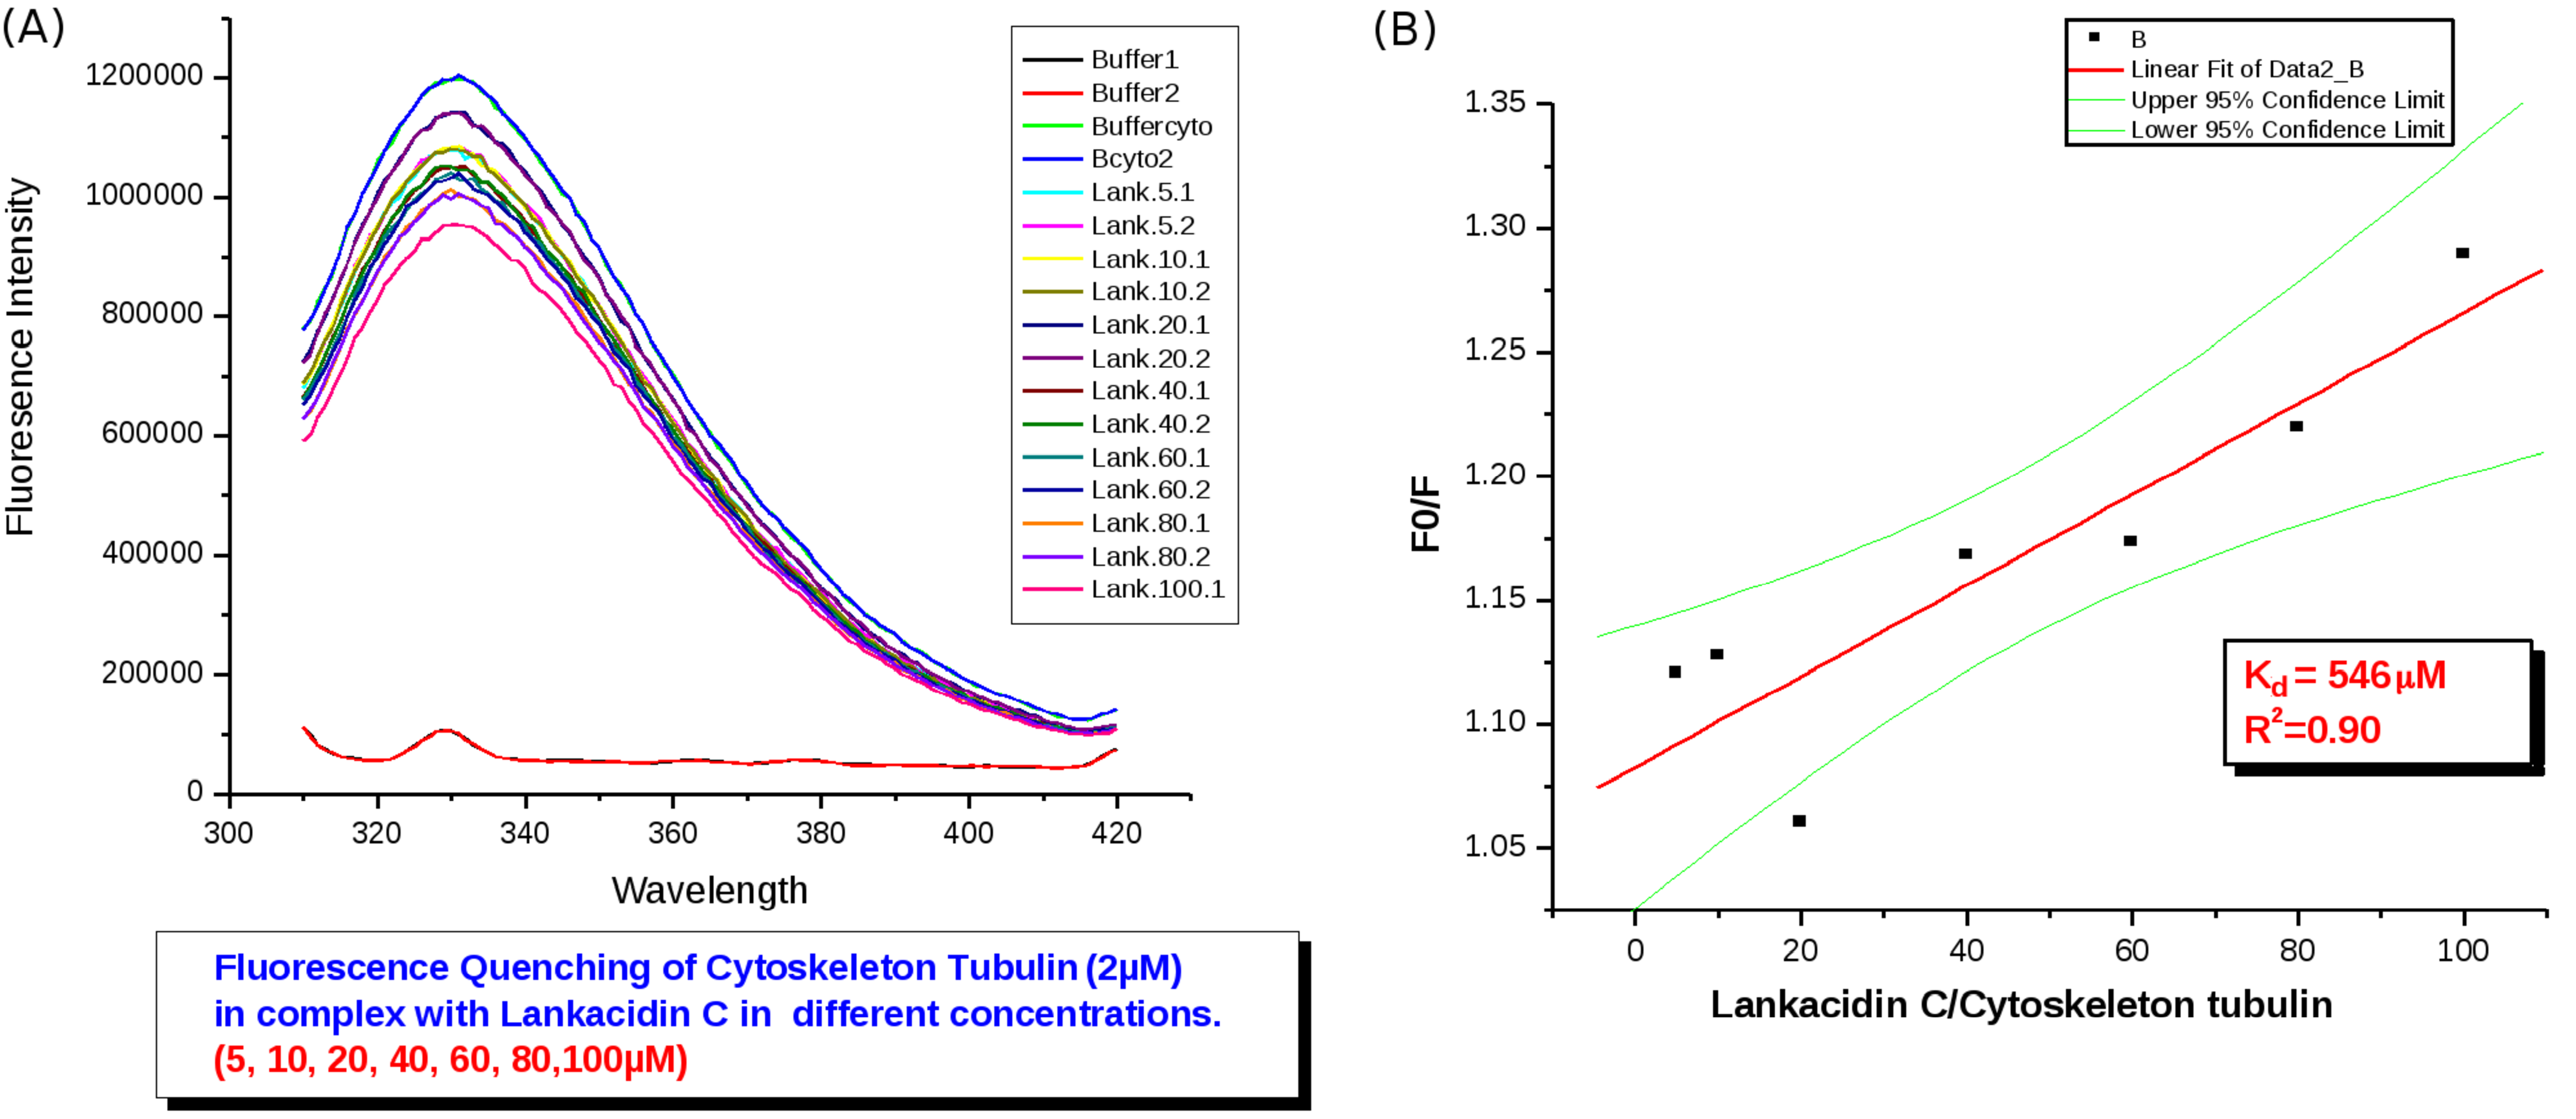
\includegraphics[width=1.0\linewidth]{images/LankC_PorcCyto.pdf}
\caption[Effect of lankacidin C on fluorescence of the porcine cytoskeleton tubulin]{ 
Effect of Lankacidin C on fluorescence of the porcine cytoskeleton tubulin using fluorescence
quenching assays.}
\label{f:Lank-LankC_PorcCyto}
\end{figure}

\begin{figure}
\centering
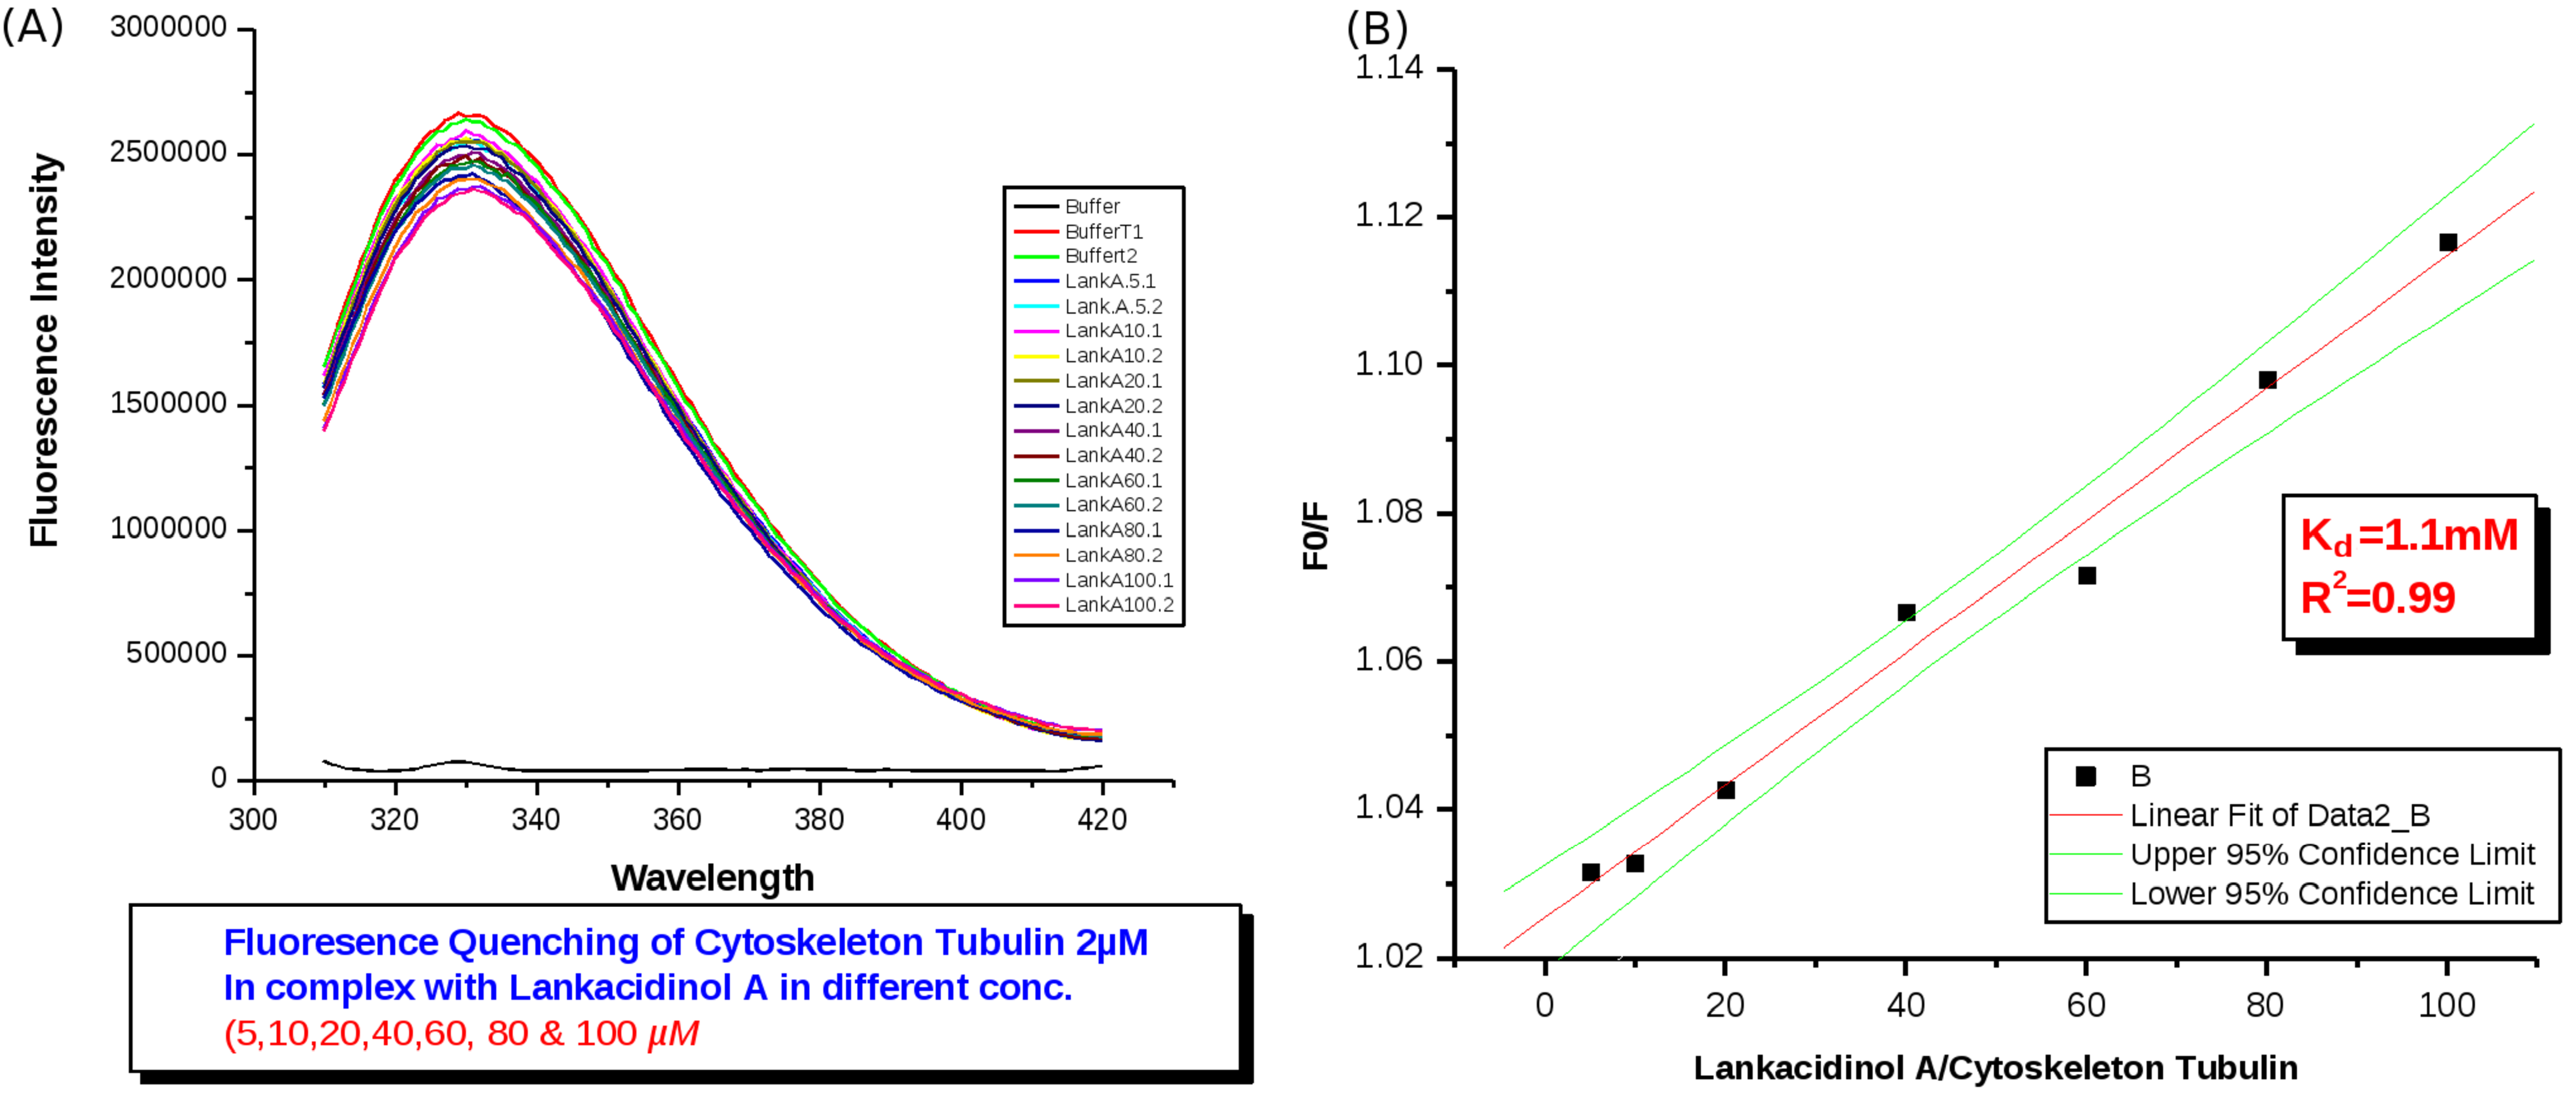
\includegraphics[width=1.0\linewidth]{images/LankA_PorcCyto.pdf}
\caption[Effect of lankacidinol A on fluorescence of the porcine cytoskeleton tubulin]{
Effect of lankacidinol A on fluorescence of the porcine cytoskeleton tubulin using fluorescence
quenching assays.}
\label{f:Lank-LankA_PorcCyto}
\end{figure}

We also tested whether lankacidins directly bind to the recombinant purified TUB-BI dimers, which would help us decide as to which tubulin subunit
lankacidins bind. Interestingly, we found that both lankacidins have binding affinities towards recombinant purified TUB-BI. 
The characteristic tubulin fluorescence emission spectrum was significantly quenched by lankacidinol A with a $K_d$ value of $654\,\mu$M versus $1.06$ mM for lankacidin C. Both are affecting the TUB-B1 conformation in a concentration-dependent manner
(see Fig. \ref{f:Lank-LankC_Recom} and Fig. \ref{f:Lank-LankA_Recom}).
These findings indicate that lankacidins have moderate effects causing
conformational changes in tubulin upon binding.
The findings also indicate that lankacidins bind to the $\beta$-tubulin
subunit, which narrows down the search for proving our hypothesis.

\begin{figure}
\centering
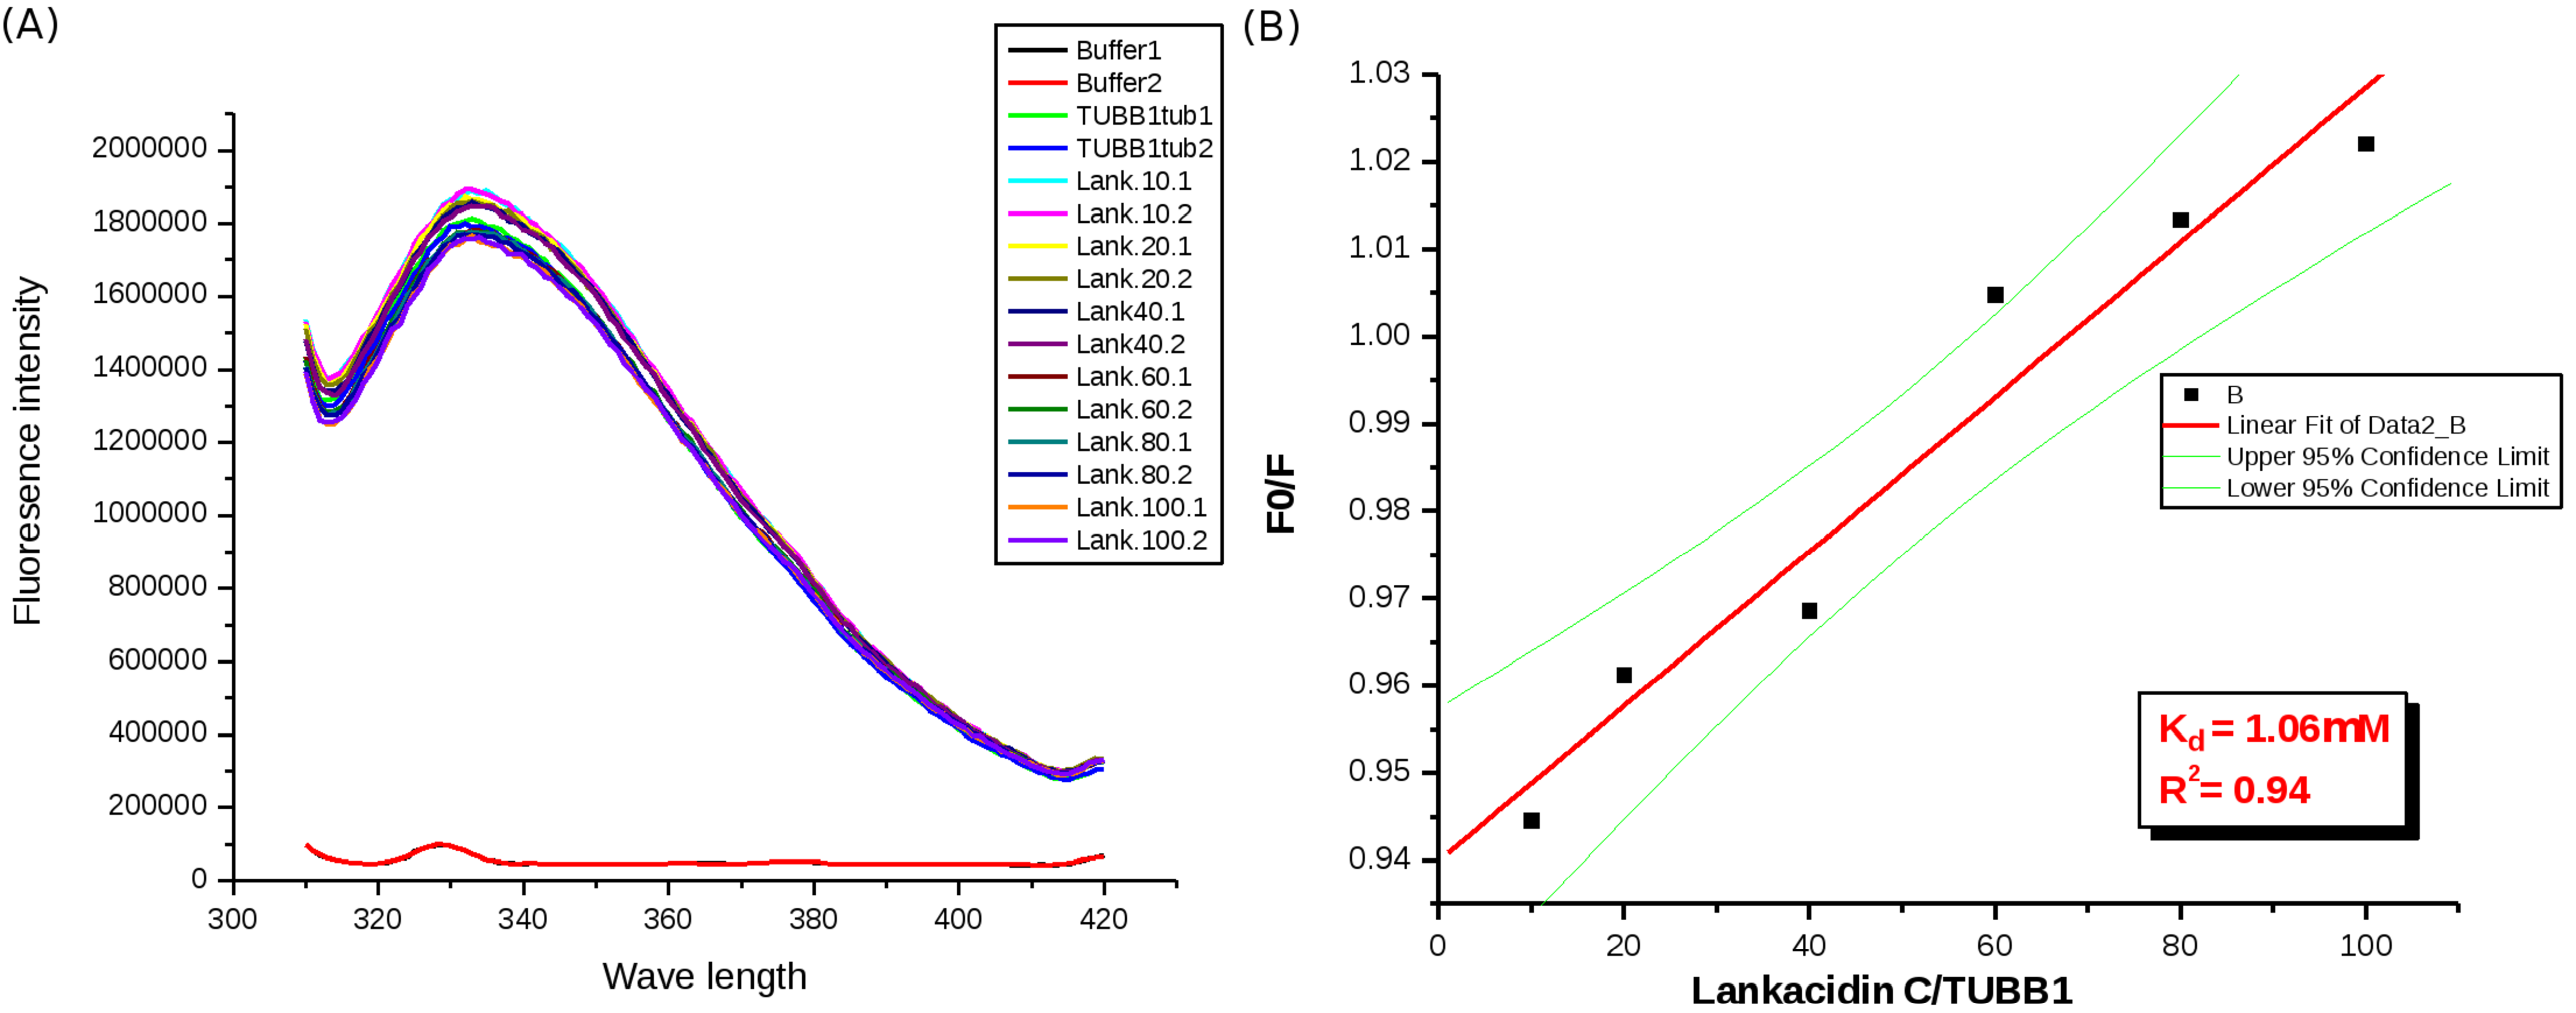
\includegraphics[width=1.0\linewidth]{images/LankC_Recom.pdf}
\caption[Effect of lankacidin C on fluorescence of purified recombinant TUB-BI]{
Effect of lankacidin C on fluorescence of purified recombinant TUB-BI using fluorescence
quenching assays.}
\label{f:Lank-LankC_Recom}
\end{figure}


\begin{figure}
\centering
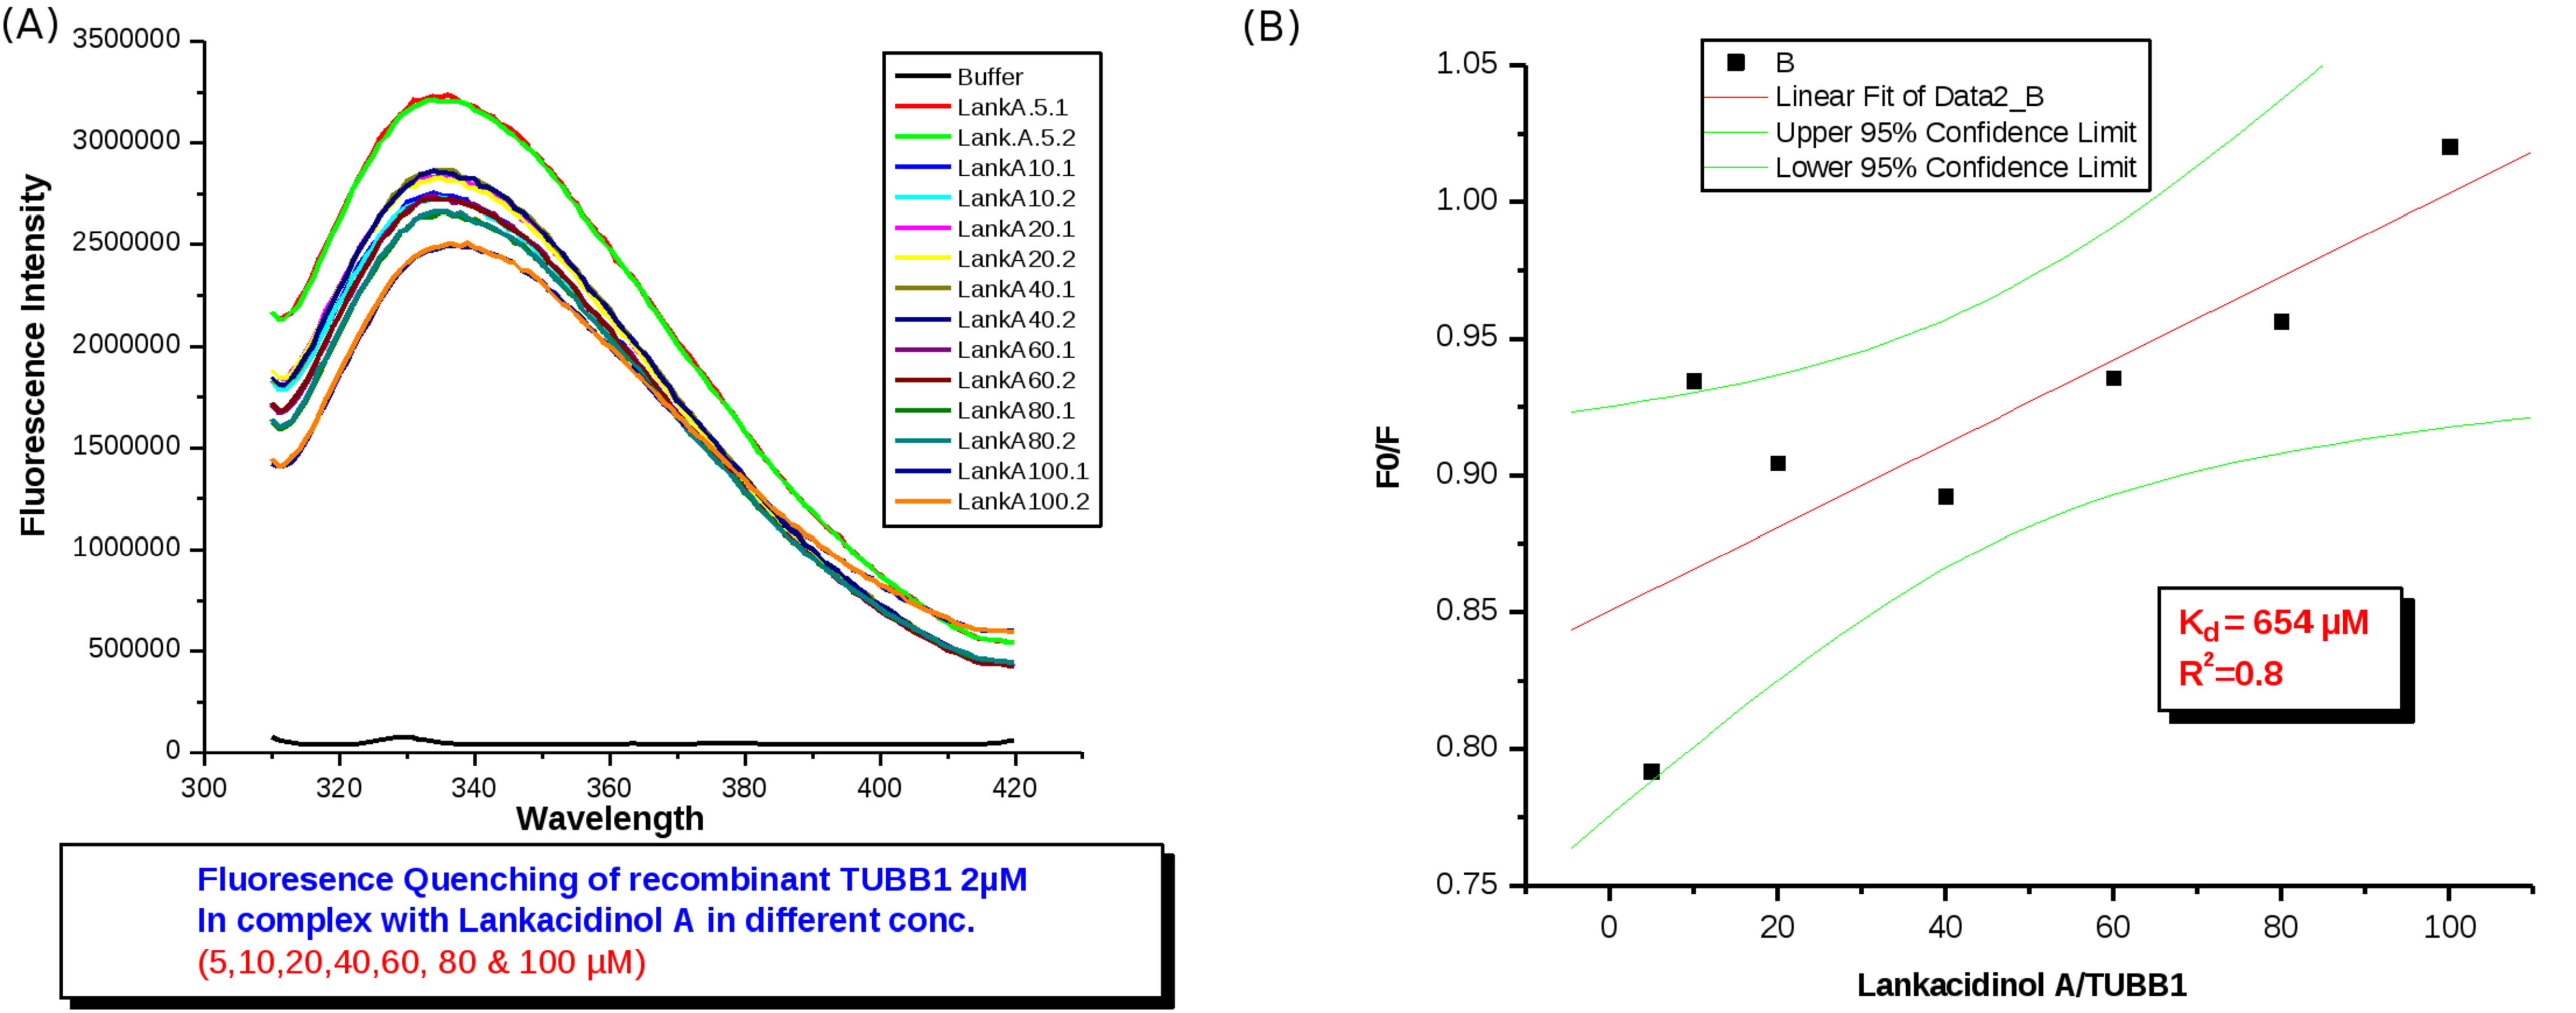
\includegraphics[width=1.0\linewidth]{images/LankA_Recom.pdf}
\caption[Effect of lankacidinol A on fluorescence of purified recombinant TUB-BI]{ 
Effect of lankacidinol A on fluorescence of purified recombinant TUB-BI using fluorescence
quenching assays.}
\label{f:Lank-LankA_Recom}
\end{figure}

\section{Discussion and Conclusions}

The present work shows an example of how computational predictions 
aid in the understanding of mechanisms of drug actions. Based on similarity to
a previous hit that was predicted to bind to the tubulin taxol binding site,
lankacidins were also predicted to bind to the same site, which 
was suggested to be the mechanism of their antitumor activity.
Computational estimation of lankacidin C binding energy to the taxol binding site
returned values that reflect relatively weak affinity, comparable to that of 
sarcodictyin A, which agrees with its relatively weak antitumor activity.  
Fluorescence quenching experiments confirmed the computational predictions
and indicated that lankacidins bind to tubulin and induce conformational changes
in a concentration-dependent manner. When fluorescence quenching experiments were conducted using recombinant TUB-BI,
a similar effect was noticed which narrows down our search to the $\beta$-tubulin
subunit where the taxol binding site is, rather than the $\alpha$-subunit.

Because this  still does not prove the hypothesis, we need to do more experiments
which should prove if lankacidin actually binds at the $\beta$-tubulin
taxol binding site or not. Currently, we are carrying out a competitive
binding assay in which the competition of lankacidins with fluorescent 
taxoid (Flutax-2) for the taxol binding site is assessed. The
results of these
experiments should shed light on whether our hypothesis 
regarding lankacidin antitumor 
mechanism of action is true or not.


\chapter{Estimating Hydrogen Bond Energies: Comparison of Methods}
\label{HB}

\footnote{A version of this chapter
was published as: A. T. Ayoub, J. Tuszynski, and M. Klobukowski, ``Estimating hydrogen bond energies: comparison of methods,'' 
\emph{Theoretical Chemistry Accounts}, vol. 133, issue 8,
1520-1527, 2014} 

\section{Summary}
Hydrogen bonds are among the most important non-bonded interactions found in molecules. Different methods of estimating the strength of hydrogen bonds have been proposed to date. In this work, we present a comparison between methods of estimating hydrogen bond energies that are based on several electron density descriptors based on the quantum theory of atoms in molecules, the natural bond orbital theory, and Mulliken population analysis. The results indicate that the most powerful approach is based on the quantum theory of atoms in molecules, followed by the one employing the natural bond orbital theory. The Mulliken population analysis performed very poorly. The effect of including dispersion correction was also studied. Parameters for predicting hydrogen bond energies are presented.

\section{Introduction}
\label{s:HBP-Intro}

The hydrogen bond is an important type of non-bonded interactions, which comprises a strong electromagnetic dipole-dipole interaction between polar molecules. The interaction takes place between a hydrogen bond donor, which is a hydrogen atom attached to a highly electronegative atom, and a hydrogen bond acceptor, which is another highly electronegative atom. Electronegative atoms involved in hydrogen bonding are usually oxygen, nitrogen, and fluorine
\cite{Arunan2011-1,Arunan2011-2,Desiraju2002}. 
Hydrogen bonds are also important in forming the secondary and tertiary structures of proteins and the stability between subunits in multimeric proteins\cite{Deechongkit2004,Rose2006,Hellgren2007}. 
Therefore, a facile way of estimating the strength of hydrogen bonds could be very useful. The electron density distribution around the atoms involved in the formation of a hydrogen bond, and other bonds like covalent bonds, have been shown to correlate with the bond strength
\cite{Davidson1967,Roby1974,Ehrhardt1985}, 
and be a strong predictor of hydrogen bond strength
\cite{Reiher2001,Thar2006,Schmidt2008,Schenk2008,Grabowski2001,Gora2005,Parthasarathi2005,Parthasarathi2006,Gatti1994}.

There are several methods of characterizing the electron
density distribution in hydrogen-bonded systems. Among these methods are the quantum theory of atoms in molecules (QTAIM)
\cite{Bader1990,Bader1991}, the natural bond orbital population analysis
\cite{Glendening2012}, and the Mulliken population analysis
\cite{Mulliken1955}.
In QTAIM, the electron density at the bond critical
point ($\rho$) is a useful measure of bond strength. A bond critical point is a point along the bond coordinate that has a zero gradient of the electron density distribution
\cite{Bader1990,Bader1991}. 
This quantity, $\rho$, has been shown to correlate with bond strengths
\cite{Grabowski2001,Gora2005,Parthasarathi2005,Parthasarathi2006,Gatti1994,Grabowski2000,Alkorta1998}. In natural bond orbital population analysis
\cite{Glendening2012}, there are two quantities that are similar in concept and are also expected to correlate with the strength of the bonds. These two quantities are \gls{WBI}
\cite{Wiberg1968} and the \gls{OWBO}
\cite{Reed1983,Reed1985} 
between the hydrogen atom and the hydrogen bond acceptor atom, both calculated in natural atomic orbital basis
\cite{Glendening2012}. 
Finally, in the Mulliken population analysis
\cite{Mulliken1955}, 
the \gls{MOC} between the interacting atoms was also shown to correlate with bond strengths
\cite{Ehrhardt1985}. In the present study, all these quantities, namely $\rho$, WBI, OWBO, and MOC, were assessed for relationship with strength of hydrogen bonds to establish which one leads to a better correlation. Dispersion correction and basis set effects were also characterized.

Two quantum chemical approaches are available to
calculate the strength of a hydrogen bond between two molecules, the supermolecular approach and intermolecular perturbation theory
\cite{Scheiner2007,Jeziorski2002}. In the supermolecular approach, the one adopted here, the interaction energy between two molecules A and B, is calculated as
\begin{equation}
\label{eq:HBP-superMol}
 E_{I}\left(\mathbf{r_{A}},\mathbf{r_{B}}\right) =  
 E_{AB}\left(\mathbf{r_{A}},\mathbf{r_{B}}\right) -  E_{A}\left(\mathbf{r_{A}}\right) 
 -  E_{B}\left(\mathbf{r_{B}}\right)
\end{equation}
where  $\mathbf{r_{A}}$ and $\mathbf{r_{B}}$ denote the coordinates of the atoms in molecules A and B, respectively. $E_{AB}$ is the energy of the complex while $E_A$ and $E_B$ are the energies of molecules $A$ and $B$, respectively. Such direct evaluation of the hydrogen bond interaction energy is not always possible: either the interacting systems are too large or more than just hydrogen bonding interactions are present. It is possible to get around these obstacles by designing an interpolation formula that depends only on the electron density between the atoms involved in a hydrogen bond, that is, the hydrogen atom and the hydrogen bond acceptor atom. Parameters in such a fitting formula could be derived using known hydrogen bond energies in systems that interact only via a single hydrogen bond. This approach was followed by Thar and Kirchner who used a training set of complexes satisfying these criteria
\cite{Thar2006}. They used these molecules in designing an interpolation formula based on the two-center shared electron number in order to detect hydrogen bonds
\cite{Thar2006}. We used a subset of their training set in drawing our correlation.

\section{Methodology}
\label{s:HBP-Methods}

All the isolated hydrogen-bonded complexes, 45 in total, were optimized using the density functional theory with the B3LYP functional
\cite{Becke1993,Lee1988,Vosko1980}. A primary basis set used in this work was the triple-zeta valence polarized basis set (TZVP)
\cite{Schaeffer1992,Schaeffer1994}. Since hydrogen bond interaction energies $E_I$ were calculated in a supermolecular approach, all the energies of the isolated molecules needed to be counterpoise corrected for the basis set superposition error
\cite{Boys1970,Simon1996}. 
We employed the counterpoise correction in the calculation of the interaction energy from the optimized structure but not during the optimization process itself. 
The optimized structure was then used for QTAIM analysis, natural bond orbital population analysis, and Mulliken population analysis to extract the values of the descriptors $\rho$, WBI, OWBO, and MOC introduced before. The hydrogen bond energies in all the complexes were plotted against each of these four descriptors and the correlation was assessed. Case studies of a test set were also performed to investigate the ability of each descriptor to predict the hydrogen bond energies. In order to assess a possible effect of dispersion correction, we studied the same 45 hydrogen-bonded complexes that were already minimized at B3LYP/TZVP level of theory, using several DFT functionals as well as the M{\o}ller-Plesset perturbation theory, namely B97D functional
\cite{Grimme2006}, wB97xD functional
\cite{Jeng-Da2008,Jeng-Da20082}, 
MP2 \cite{Moller1934,HeadGordon1988,Frisch1990}, 
and the previously used B3LYP. We also checked the effect of augmenting the basis set: diffuse functions from the aug-cc-pVDZ basis set
\cite{ccpVTZ,Kendall1992} were added to the TZVP basis set (the augmented TZVP basis set was denoted aug-TZVP). The software used in the calculations was Gaussian 09
\cite{g09}. Avogadro software was used for building and viewing the molecules
\cite{Hanwell2012}.

\section{Results and Discussion}
\label{s:HBP-Results}



\begin{figure}
  \centering
  \subfloat[]{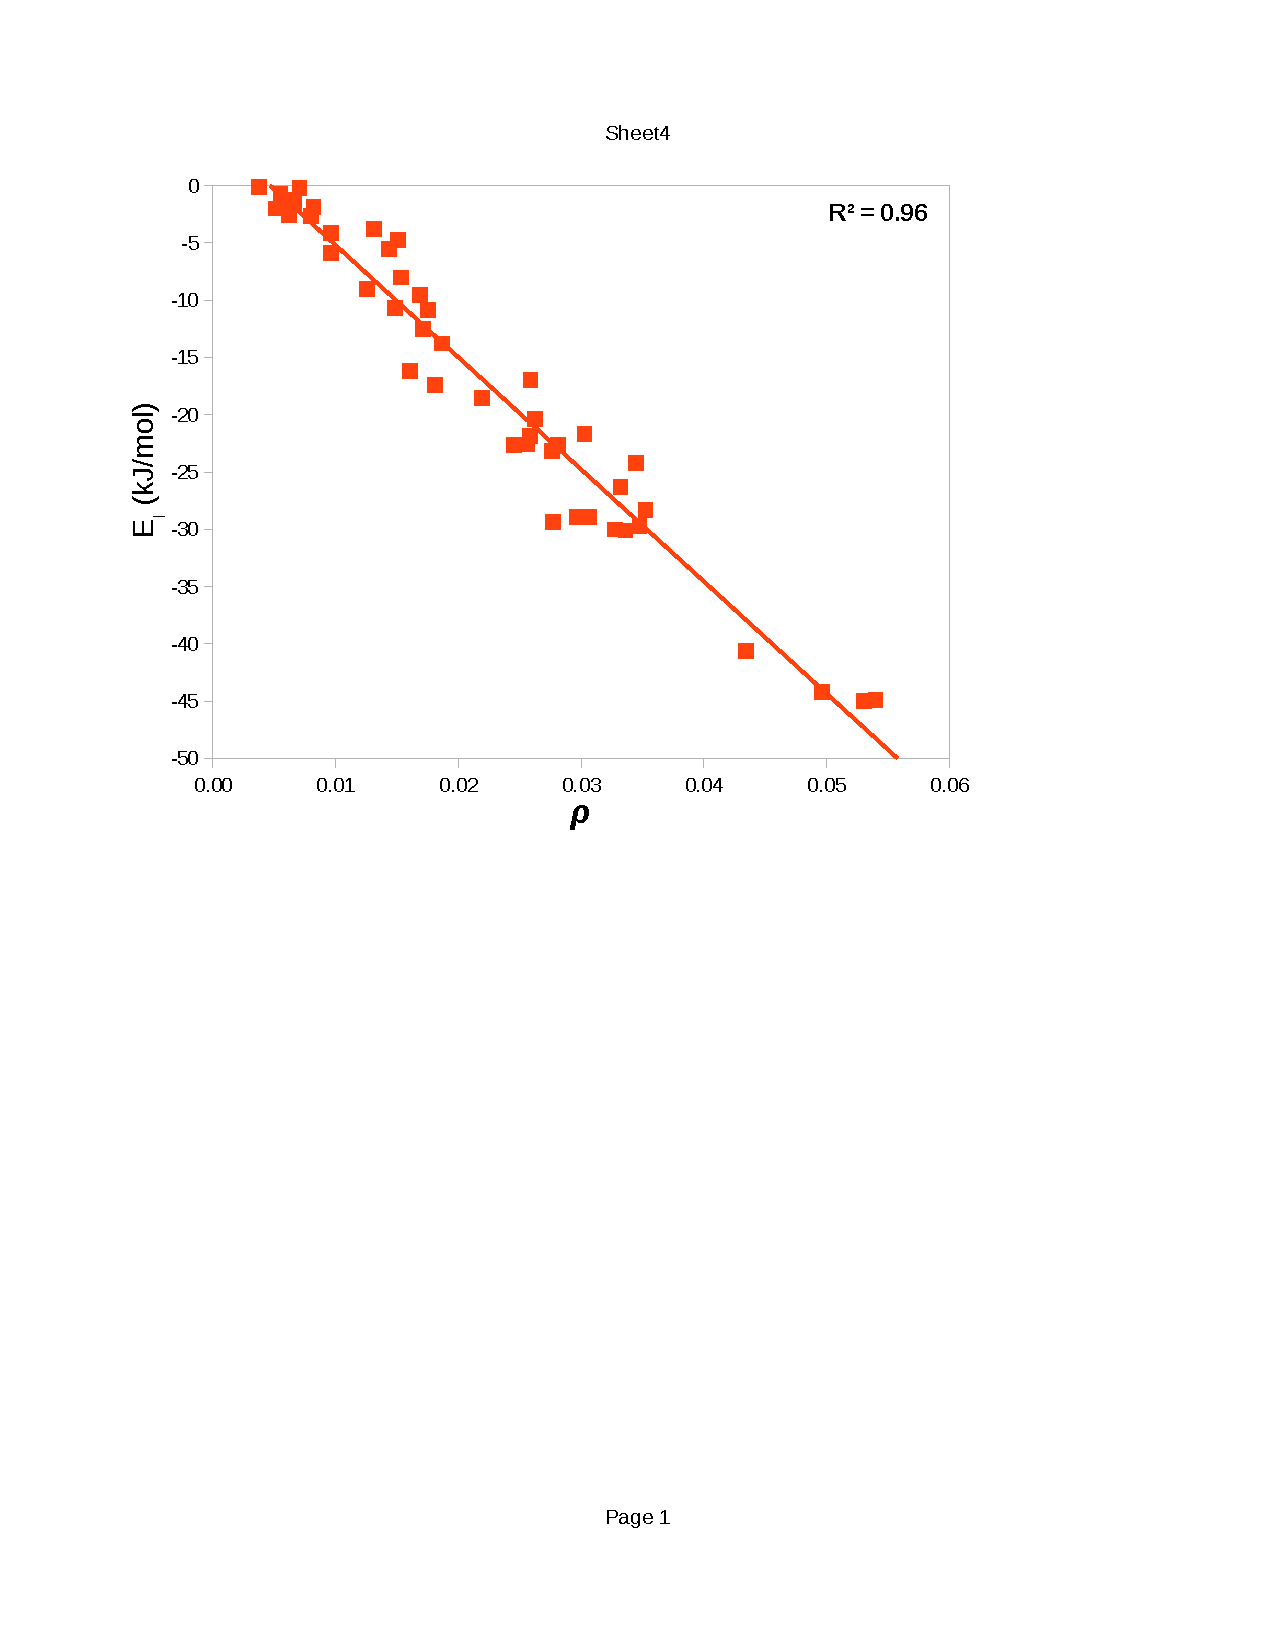
\includegraphics[width=0.48\linewidth,trim=2cm 13.5cm 5.2cm 3cm, clip=true]{images/qtaim.pdf}}
  \hspace{0.01\linewidth}
  \subfloat[]{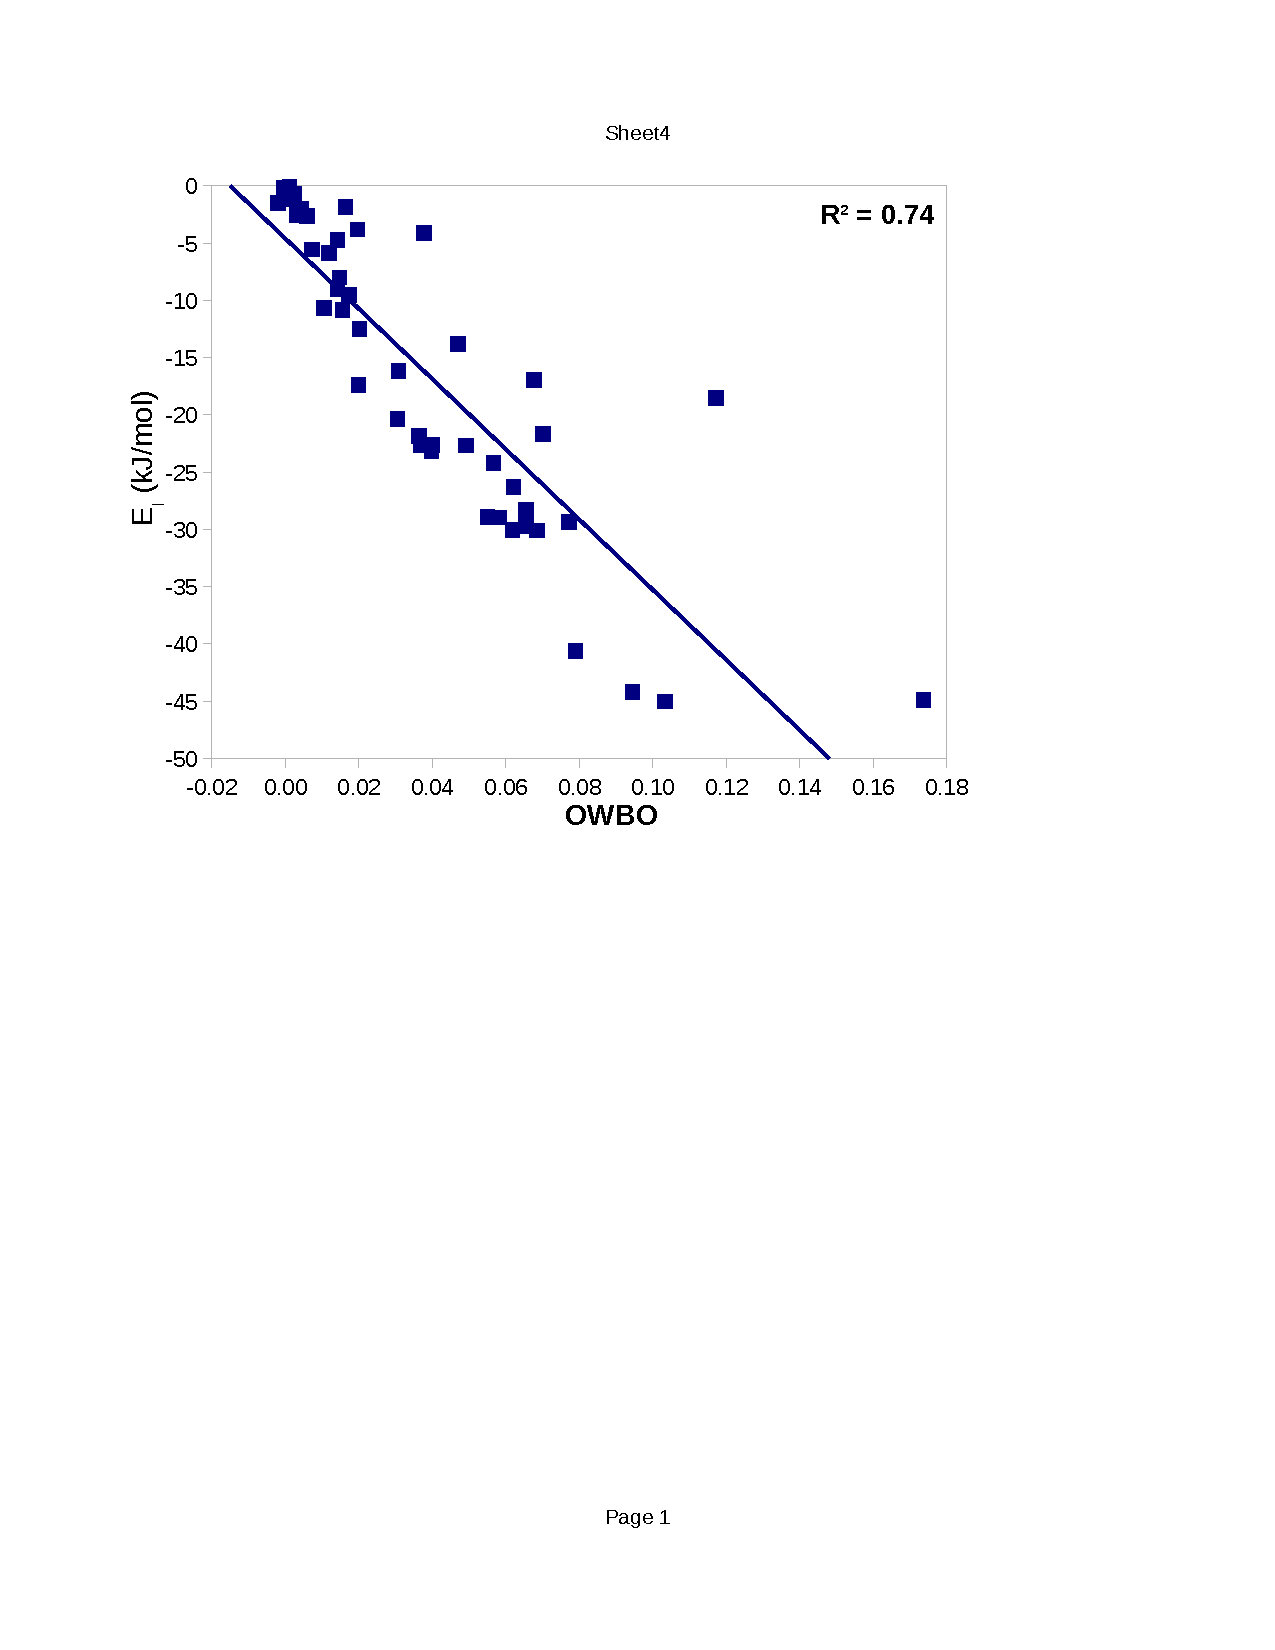
\includegraphics[width=0.48\linewidth,trim=2cm 13.5cm 5.2cm 3cm, clip=true]{images/owbo.pdf}}
  \vspace{0.01\linewidth}
  \subfloat[]{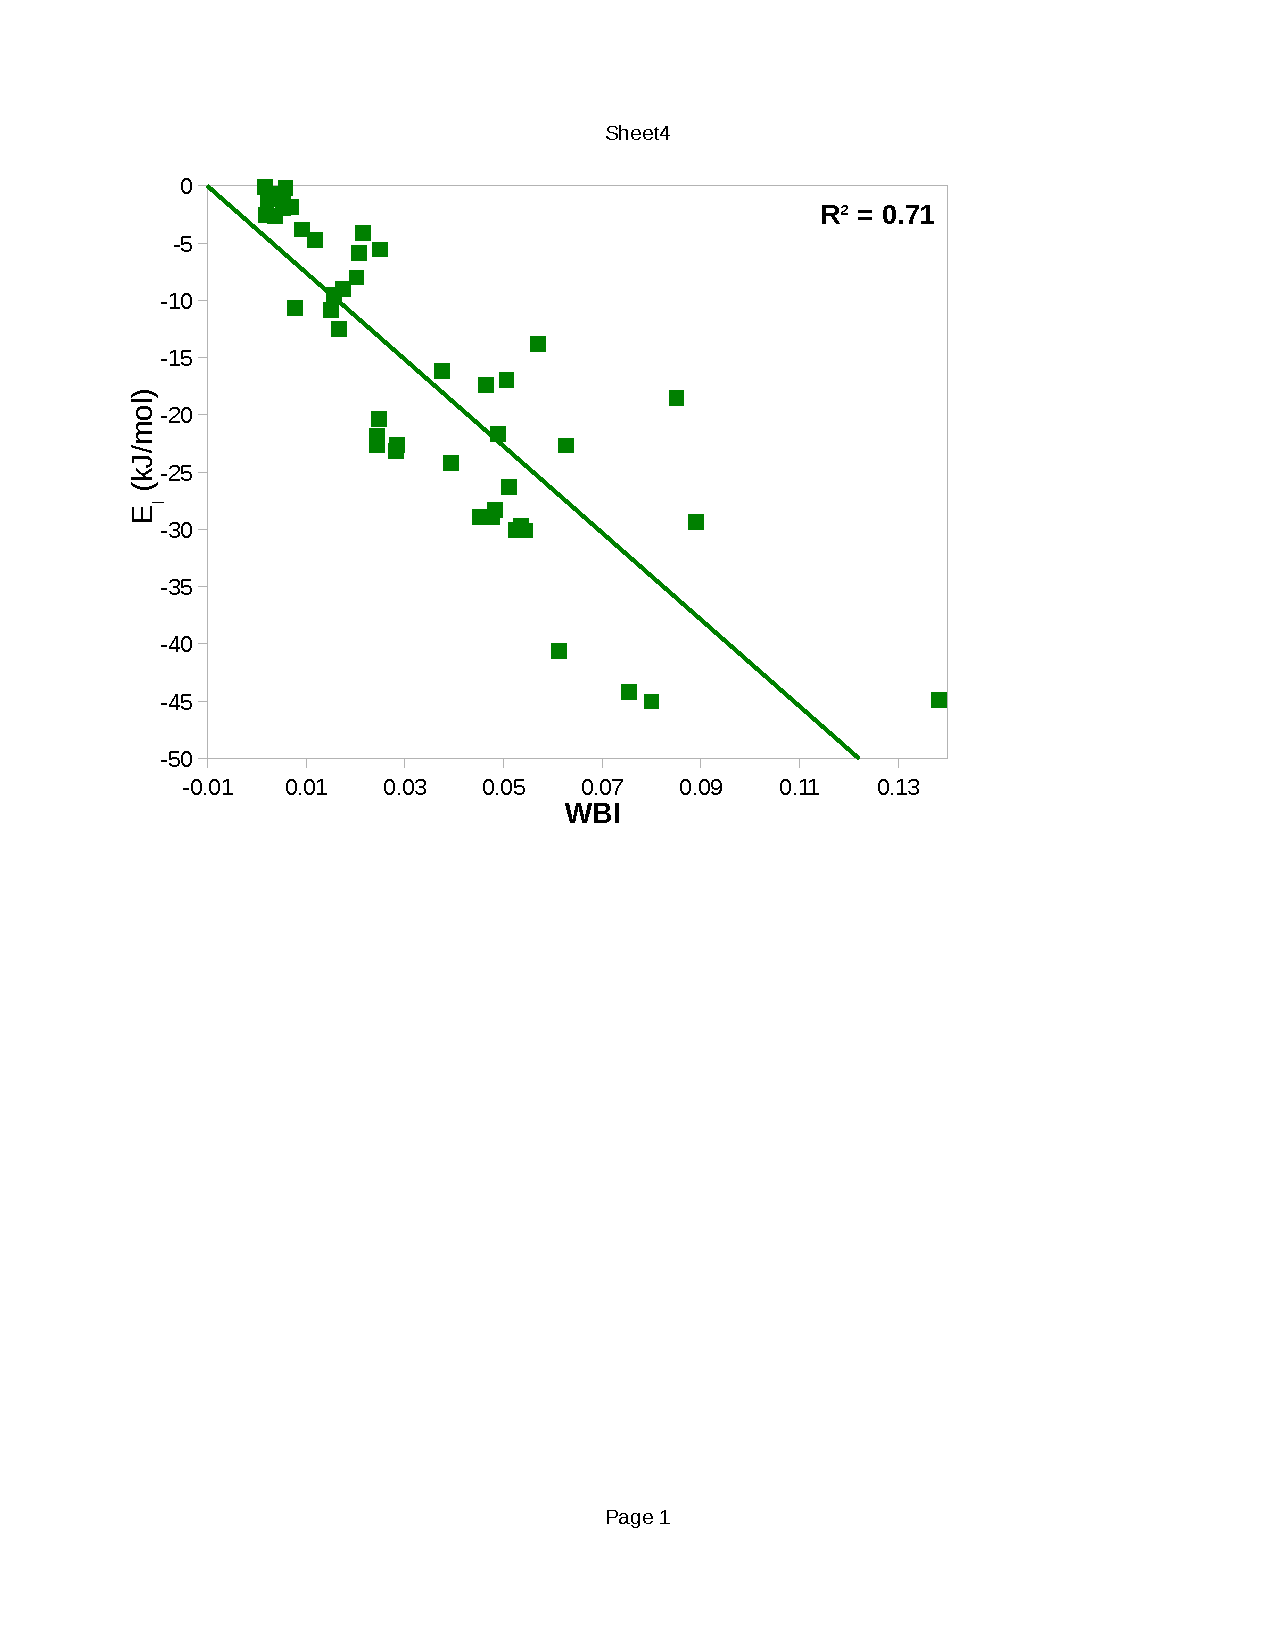
\includegraphics[width=0.48\linewidth,trim=2cm 13.5cm 5.2cm 3cm, clip=true]{images/wbi.pdf}}
  \hspace{0.01\linewidth}
  \subfloat[]{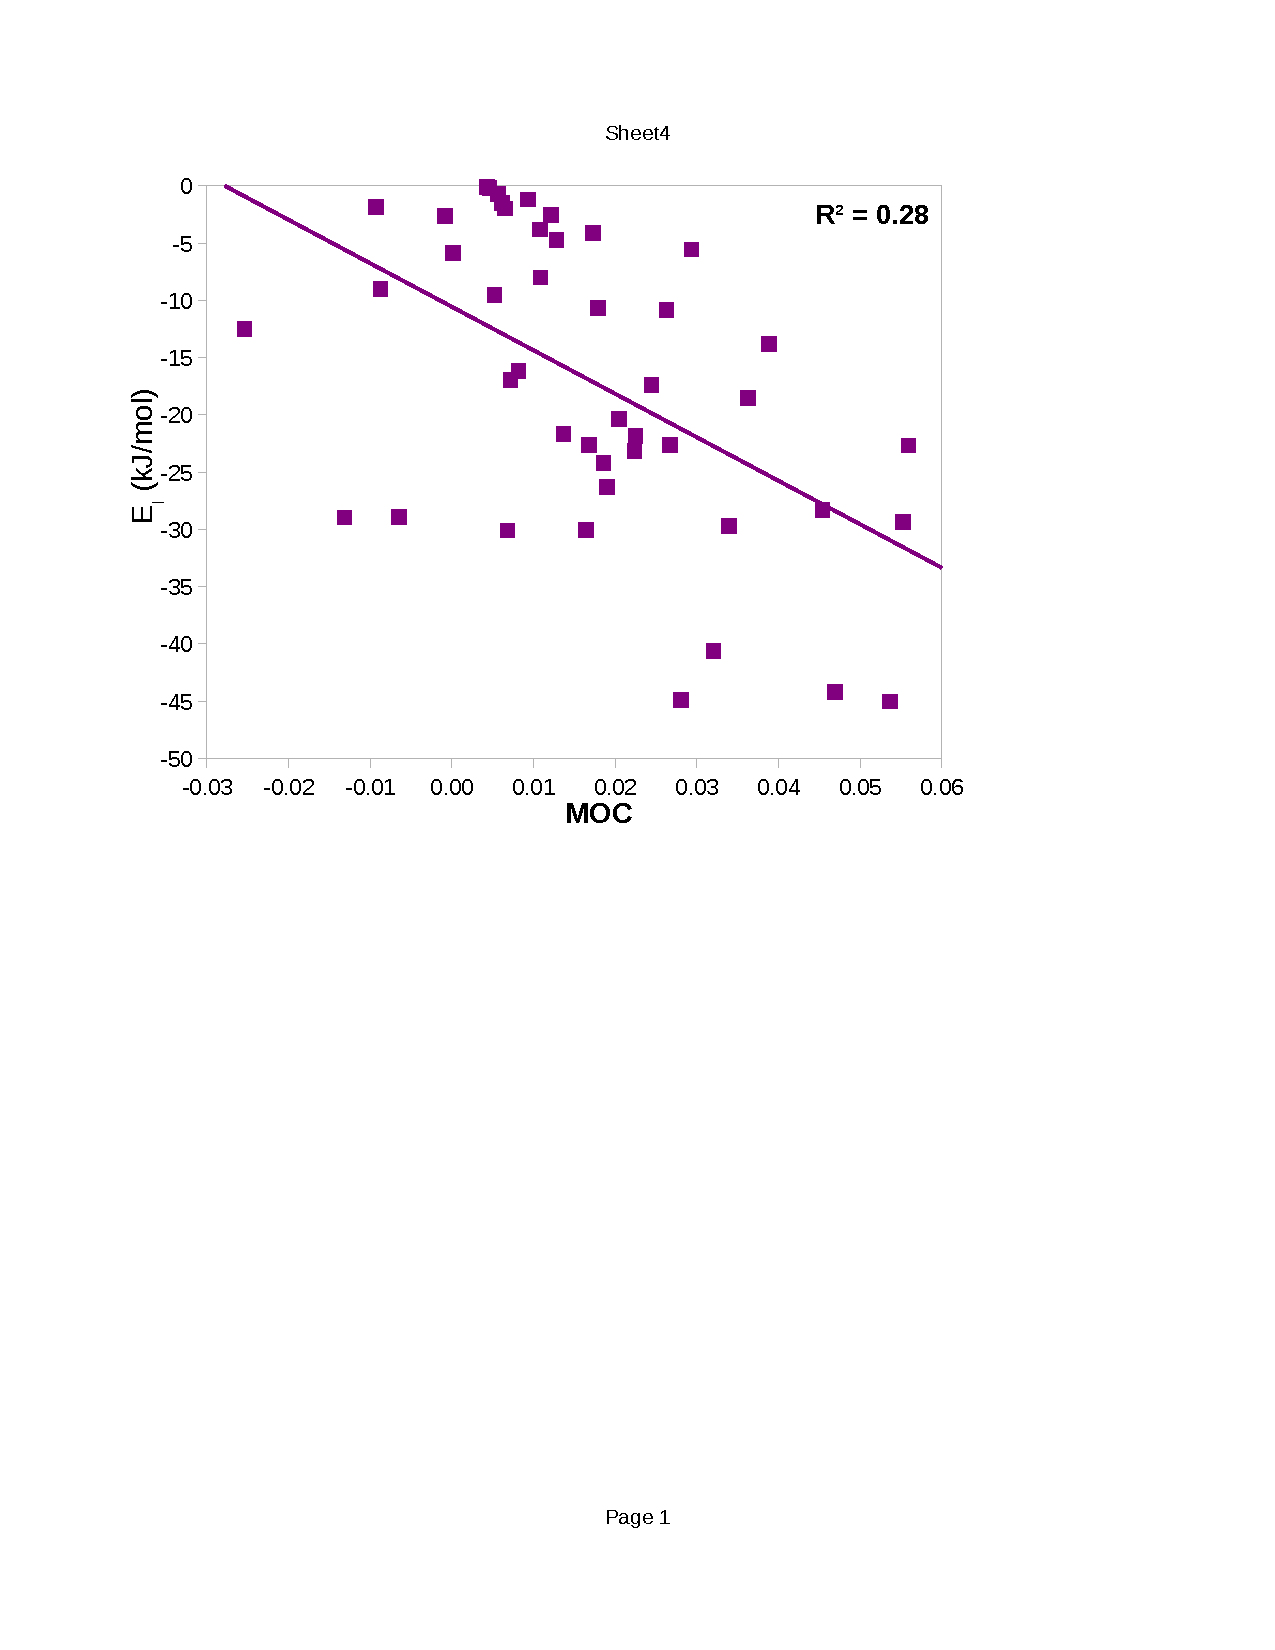
\includegraphics[width=0.48\linewidth,trim=2cm 13.5cm 5.2cm 3cm, clip=true]{images/moc.pdf}}
  \caption[Regression plots]{Regression plots of the hydrogen bond energy $E_{I}$ versus the four descriptors studied.}
  \label{f:HBP-plots}
\end{figure}
\subsection{Performance of Descriptors}
\label{ss:HBP-Res_PerfDesc}

The energies of the hydrogen bonds in the 45 hydrogen-bonded complexes as well as the values of the four hydrogen bond descriptors under study ($\rho$, WBI, OWBO, and MOC) were calculated. 
These data are included in 
Table \ref{t:S-HBP-descriptors}
in the Appendix. The optimized coordinates of all
complexes are available online in \cite{Ayoub2014HB}.
The results of the linear regression analysis are included in
Fig. \ref{f:HBP-plots}, 
and linear fitting parameters are included in 
Table \ref{t:HBP-stat}. 
As Fig. \ref{f:HBP-plots}a shows, the best correlation is obtained for the density at the
bond critical point ($\rho$) evaluated in QTAIM, with a coefficient of determination (R$^2$) of 0.96, which indicates a very strong correlation. We should point out that we used a
heterogeneous training set that contains different types of atoms as acceptors and donors including oxygen, nitrogen, fluorine, chlorine, bromine, sulfur, phosphorous, and carbon
(see Appendix). 
Consequently, the descriptor $\rho$ calculated in QTAIM analysis proves to strongly correlate with the hydrogen bond energy regardless of the types of the atoms involved in the hydrogen bond.
\begin{table}
 \caption[Linear fitting parameters at B3LYP/TZVP]{Linear fitting parameters at B3LYP/TZVP level of theory for the plots of hydrogen bond energies versus different descriptors.}
 \label{t:HBP-stat}
 \centering
 \begin{tabular*}{\linewidth}{@{\extracolsep{\fill}}lccccc}
\toprule
 Descriptor && $R^{2}$ & $m$  & $b$  & $\sigma$ \\
\midrule
 $\rho$ && 0.96	& --979	& 4.59    & 2.69 \\
 OWBO	&& 0.74	& --307	& --4.61  & 6.64 \\
 WBI	&& 0.71	& --379 & --3.80  & 6.97 \\
 MOC	&& 0.28	& --380 & --10.56 & 10.98\\
\bottomrule
 \end{tabular*}
 \vspace{-0.45cm}
 \begin{flushleft}
 $R^2$ is the coefficient of determination. $m$, $b$, and $\sigma$ are the slope, intercept, and standard deviation measured in kJ/mol, respectively.
 \end{flushleft}
\end{table}
As Table
\ref{t:HBP-stat} 
shows, the correlation with the descriptor
$\rho$ has a slope ($m$) of $-979$ kJ/mol and an intercept ($b$) of 4.59 kJ/mol. 
The standard deviation is relatively very low
($\sigma$=2.69 kJ/mol). Therefore, these regression parameters could be used in predicting the hydrogen bond energies of more complex cases only by calculating the descriptor $\rho$, or any other descriptor, and substituting into the equation:
\begin{equation}
\label{eq:HBP-fit}
  E_{I} = m {\cal D} + b 
\end{equation}
where $m$ is the slope, $\cal D$ is the descriptor value, and $b$ is the intercept. 

The three remaining plots in 
Fig. \ref{f:HBP-plots} 
demonstrate
that the three other approaches to estimating hydrogen bond energies exhibit a much lower degree of correlation
than the one based on $\rho$. The overlap-weighted bond order (OWBO) from natural population analysis displays a correlation with an $R^2$ of 0.74 
(Fig. \ref{f:HBP-plots}b) similar to the Wiberg bond index (WBI) correlation with an $R^2$ value of 0.71. Thus, the natural population analysis still provides good descriptors for predicting hydrogen bond energies, although not as good as QTAIM. The fitting parameters of the linear regression for OWBO and WBI have very similar values. However, despite the lower quality of the correlation, the values of $m$ and $b$ derived for natural bond orbital descriptors may be useful in predicting hydrogen bond energies according to 
Eq.\ref{eq:HBP-fit}. 
Fig. \ref{f:HBP-plots}d shows that the Mulliken overlap charge (MOC) exhibits the poorest correlation with the hydrogen bond energies, with an $R^2$ value of only 0.28. Moreover, the standard deviation $\sigma$ is very high, 10.98 kJ/mol. Therefore, we do not recommend using the descriptor MOC in predicting the hydrogen bond energies. It should be mentioned that MOC values are
sometimes negative, devoid of a physical sense. This happens even for hydrogen bonds that are actually very strong (see Fig. 
\ref{f:HBP-plots}d and Table \ref{t:S-HBP-descriptors}). 
This behavior can also be seen in the case of OWBO, but only in fairly rare situations for very weak hydrogen bonds (see Fig. \ref{f:HBP-plots}b and Table \ref{t:S-HBP-descriptors}). 
However, the values of $\rho$ and WBI are always positive. In particular, the values of $\rho$ would either be positive, when a hydrogen bond was present, even weak ones, or they would be zero in the absence of hydrogen bonds. Therefore, we recommend that the QTAIM-based descriptor $\rho$ be used for the best predictions of hydrogen bond energies. It should be mentioned that Parthasarathi et al. also established a strong correlation between $\rho$ and hydrogen bond energy
\cite{Parthasarathi2006}. 
However, the training set they used was relatively small (28 hydrogen bonding systems), and it spanned a huge range of energies up to nearly
$-200$ kJ/mol. We should point out that the inclusion of such very strong hydrogen bonds in the correlation analysis
weakens its predictive power and increases the deviations, especially for moderate or weak hydrogen bonds. Since in this study we aimed at developing a reliable method for predicting the energies of biologically relevant hydrogen bonds, we used a larger training set and focused on hydrogen bonds with weak to moderate strength.
\begin{figure}
  \centering
  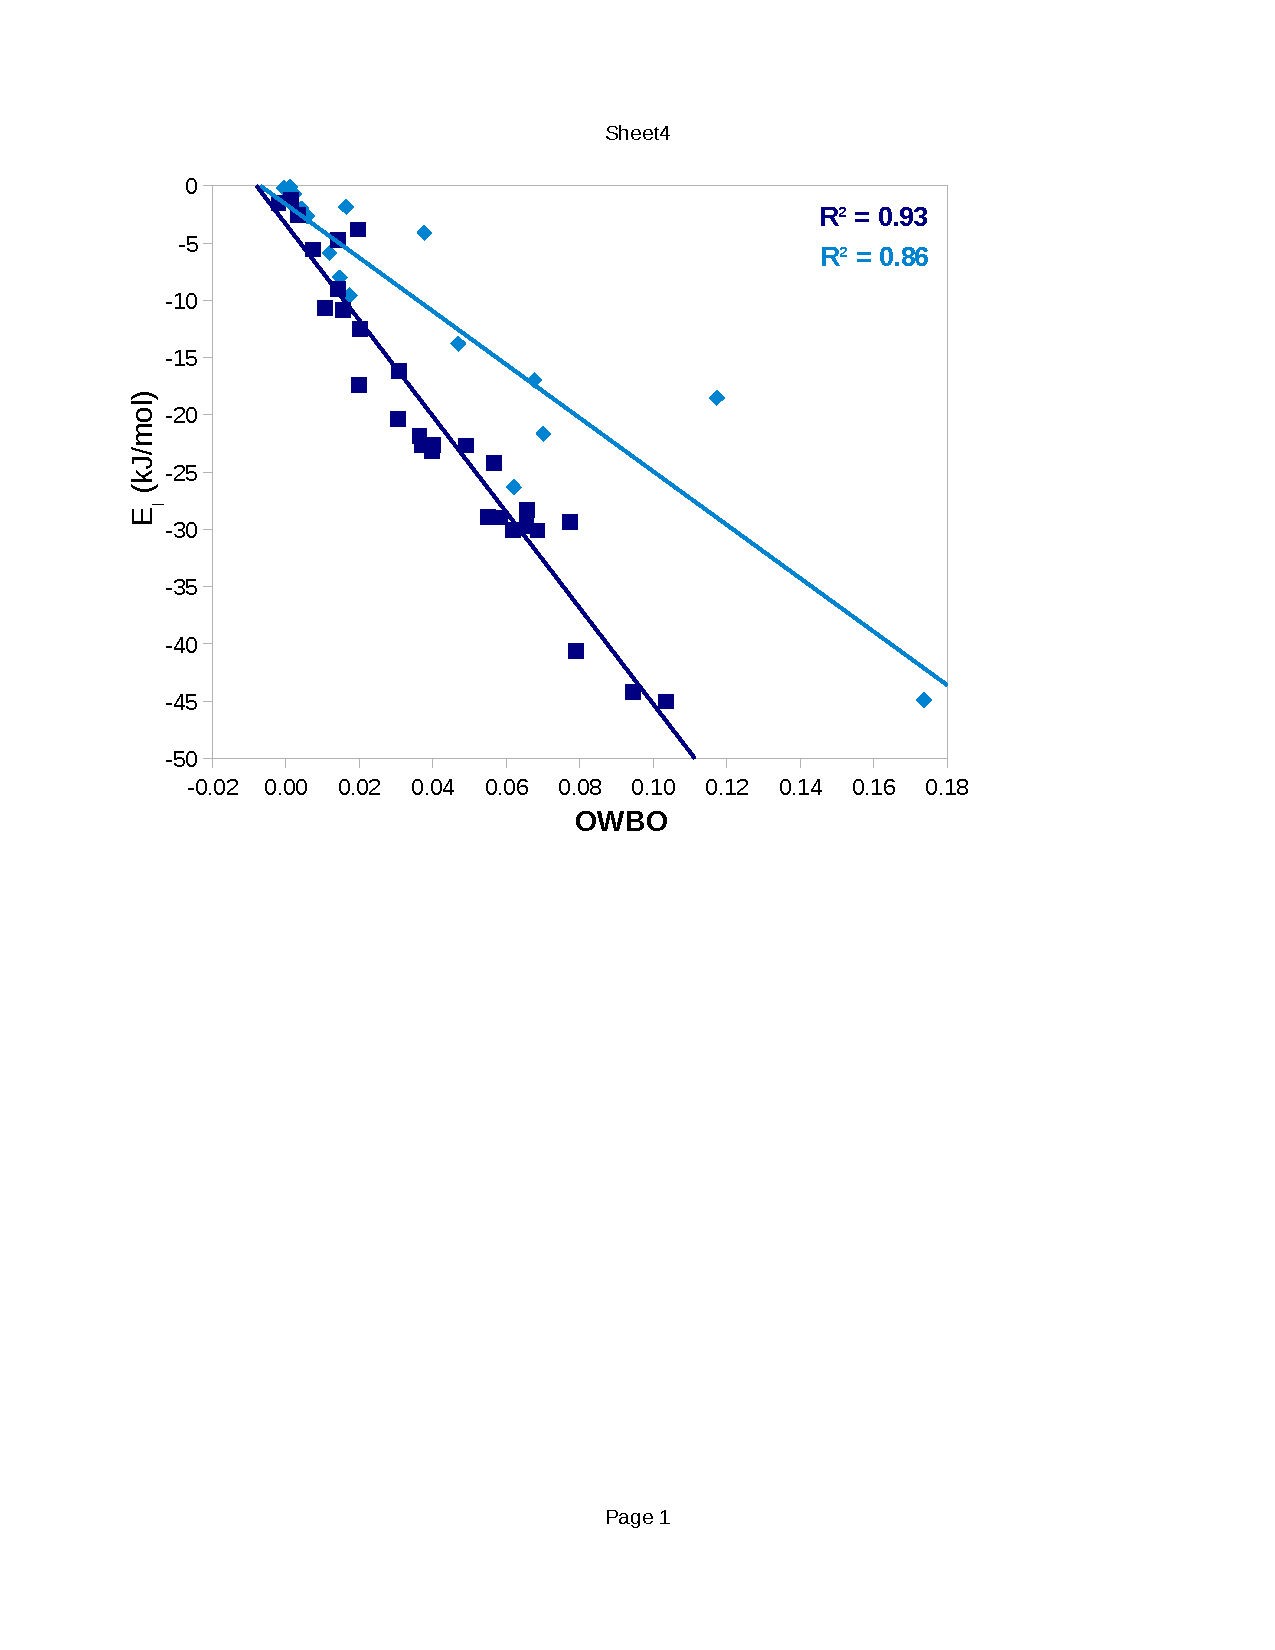
\includegraphics[width=0.65\linewidth,trim=2cm 13.5cm 5.2cm 3cm, clip=true]{images/owbo_opt.pdf}
   \caption[Improvement of OWBO descriptor performance]{Improvement of OWBO descriptor performance
   after subdivision of training set based on polarizability of
   the hydrogen bond donor.}
  \label{f:HBP-owbo_imp}
\end{figure}


Inspection of Fig. \ref{f:HBP-plots}b reveals that most of the data are
clustered nicely in a straight line with a much better correlation. However, some of the data points deviate from that line. As shown in Fig.
\ref{f:HBP-owbo_imp}, all the hydrogen-bonded complexes that had a highly polarizable hydrogen bond donor, namely sulfur, phosphorous, bromine, and chlorine, appeared to deviate largely from the other data points. We carried out a separate regression analysis for this group. The results show that, within the applied level of theory, the hydrogen-bonded complexes with non-polarizable hydrogen bond donors have a strong correlation with OWBO with an $R^2$ of 0.93, while those with highly polarizable hydrogen bond donors have a correlation with a respectable $R^2$ value of 0.86 with hydrogen bond energy. Linear fitting parameters for the two cases are shown in Table
\ref{t:HBP-OWBO2}. We tried to use the same approach with WBI but in that case the data points are scattered more randomly than in the OWBO plot. Similarly, the MOC correlation could not be improved since data points are very scattered.
\begin{table}
 \caption[Linear fitting parameters of improved OWBO descriptor]{Linear fitting parameters of improved OWBO descriptor versus hydrogen bond energies
 with polarizable (P) and non-polarizable (NP) hydrogen bond donors.}
 \label{t:HBP-OWBO2}
 \centering
 \begin{tabular*}{\linewidth}{@{\extracolsep{\fill}}lccccc}
\toprule
 Descriptor && $R^{2}$ & $m$ & $b$ & $\sigma$ \\
\midrule
 OWBO (NP)&& 0.93	& --419	& --3.36  & 3.16 \\
 OWBO (P)&& 0.86	& --233 & --1.61  & 4.49 \\
\bottomrule
 \end{tabular*}
 \vspace{-0.45cm}
  \begin{flushleft}
  $m$, $b$, and $\sigma$ are given in kJ/mol.
  \end{flushleft}
\end{table}


To test the predictive power of these models, we carried
out several case studies for more complex systems. We calculated the hydrogen bond energies using the supermolecular approach and compared them to the energies predicted via the four quantum mechanical descriptors studied here. We used the linear fitting parameters in Tables 
\ref{t:HBP-stat} and \ref{t:HBP-OWBO2} 
together with 
Eq. \ref{eq:HBP-fit}. The results of the case studies are shown in 
Table \ref{t:HBP-caseStud}. 
It should be noted that ``OWBO$_{imp}$'' refers to the energies predicted through the parameters of the improved
OWBO fit as shown in Table 
\ref{t:HBP-OWBO2}. 
Comparison of the results shows that the most accurate descriptor is $\rho$ from the QTAIM method. The results obtained with this descriptor are closest to the energies obtained via the supermolecular approach, and they lead to the lowest mean absolute error. The descriptors OWBO, WBI, and MOC perform poorly in predicting hydrogen bond energies. However, the descriptor MOC is not as bad as could be expected from its $R^2$ value in 
Fig. \ref{f:HBP-plots}d. 
Its performance is comparable to that of OWBO and WBI. This behavior of the MOC descriptor becomes clear after comparing the plots for OWBO and WBI in 
Fig. \ref{f:HBP-plots}. 
The two plots show that most of the data points are below the regression line, especially in OWBO. In OWBO, the points that are below the regression line belong to the systems that have non-polarizable hydrogen bond donors. However, the systems that have polarizable hydrogen bond donors are far above the regression line. This is manifested by most of the OWBO predictions being underestimated (see Table \ref{t:HBP-caseStud}), 
since they involve non-polarizable hydrogen bond donors.
Only the last two cases (HSH-Pyridine and HCl-Pyridine) are exceptions, which are predicted to be grossly overestimated since they involve polarizable hydrogen bond donors. It is, however, clear that the OWBO$_{imp}$ descriptor resolved this overestimation and made predictions very close to the $E_I$ values. This underscores the importance of the distinction between polarizable and non-polarizable hydrogen bond donors in the OWBO$_{imp}$ descriptor in Table
\ref{t:HBP-OWBO2}. 
This makes the OWBO$_{imp}$ descriptor the second most accurate one after $\rho$ in the QTAIM method. It should however be made clear that all the descriptors may start to fail in systems that have hydrogen bond energies outside the training set range. This is clear through the large errors introduced in the predictions of the hydrogen bond energy in the HCl-Pyridine system, which is outside the training set energy range. A good application of this hydrogen bond energy prediction scheme was found in an unpublished study that we performed using these parameters. The QTAIM parameters of the descriptor $\rho$ were used to assess the strength of hydrogen bonds that bring tubulin subunits together in microtubule cylinders. The study provided an important insight into the energetics of tubulin assembly
\cite{Ayoub2014}. The study is presented in Chapter \ref{THB}.
\begin{table}
\small
 \caption[Case studies]{Case studies implementing the linear fit parameters for the different descriptors in predicting the hydrogen bond energies.}
 \label{t:HBP-caseStud}
 \centering
 \begin{tabular*}{\linewidth}{@{\extracolsep{\fill}}>{\arraybackslash}m{3.02cm}>{\centering\arraybackslash}m{0.81cm}>{\centering\arraybackslash}m{1.98cm}>{\centering\arraybackslash}m{1.98cm}>{\centering\arraybackslash}m{1.9cm}>{\centering\arraybackslash}m{2.0cm}>{\centering\arraybackslash}m{2.1cm}}
\toprule
Complex & $E_{I}$ & $\rho$ & WBI & MOC & OWBO & OWBO$_{imp}$\\
 \midrule
 MeOH--MeF & --13.5 & --12.8 (0.7) & --8.1 (5.4) & --17.2 (--3.7) & --10.9 (2.6)& --11.9 (1.6)\\
 EtOH--EtOH & --22.2 & --22.5 (--0.3)& --14.4 (7.8) & --20.2 (2.0) & --16.7 (5.5) & --19.8 (2.3)\\
 HOH--Pyridine & --27.1 & --25.0 (2.1) & --18.9 (8.2)& --18.8 (8.3) & --19.7 (7.3) & --24.0 (3.1)\\
 MeOH--Pyridine & --26.8 & --25.6 (1.2) & --19.3 (7.5) & --19.7 (7.1) & --20.7 (6.2) & --25.3 (1.6)\\
 HCOOH--HCOOH\textsuperscript{\emph{a}}& --37.1 & --40.2 (--3.1)  & --35.3 (1.9) & --34.2 (2.9) & --33.3 (3.8) & --42.5 (--5.4)\\
 AcOH--AcOH\textsuperscript{\emph{a}}& --39.0 & --41.9 (--3.0) & --36.4 (2.6) & --35.2 (3.7) & --34.5 (4.4) & --44.2 (--5.3)\\
 Uracil--Uracil\textsuperscript{\emph{a}} & --22.0 & --21.9 (0.1) & --17.4 (4.6) & --24.6 (--2.6) & --18.4 (3.6) & --22.2 (--0.2)\\
 HSH-Pyridine & --14.9 & --17.3 (--2.5) & --17.6 (--2.8) & --14.4 (0.5) & --20.8 (--5.9) & --13.9 (1.0)\\
 HCl-Pyridine & --48.4 & --60.6 (--12.2)& --64.2 (--15.8) & --29.7 (18.7) & --61.6 (--13.2)& --44.9 (3.5)\\
 MAE \textsuperscript{\emph{b}} & NA & 2.6 & 5.5 & 4.9 & 5.4 & 2.9\\
\bottomrule
 \end{tabular*}
 \vspace{-0.45cm}
  \begin{flushleft}
	OWBO$_{imp}$is the improved fit of the OWBO descriptor. Energies in kJ/mol, and errors in parenthesis.\\
  \textsuperscript{\emph{a}} Energies per hydrogen bond are shown since these molecules have more than one hydrogen bond.\\
  \textsuperscript{\emph{b}} Mean absolute error
  \end{flushleft}
\end{table}

\subsection{Effect of Dispersion}
\label{ss:HBP-Dispersion}

We have only considered one level of theory (B3LYP density functional) and one basis set (TZVP) because we aimed at a simple yet reliable level of theory that is applicable for large systems, such as proteins
\cite{Ayoub2014}. 
However, it is prudent to compare this level of theory to models that include dispersion as well as compare the TZVP basis set with one that includes diffuse functions. 
Table \ref{t:HBP-statall} shows the linear fitting parameters for several different levels of
theory for every descriptor. Comparison of data in Tables 
\ref{t:HBP-stat} and \ref{t:HBP-statall} 
reveals that regardless of the level of theory, the descriptors vary similarly: the linear fitting parameters do not change significantly by augmenting the basis set or changing the level of theory. Specifically, comparison of
the B3LYP results in 
Tables \ref{t:HBP-stat} and \ref{t:HBP-statall}
reveals the effect of larger basis set on the descriptors. It is interesting to note that the MOC results change the most, reflecting known dependence of the results from Mulliken population analysis on quality of the basis sets, in particular on the presence of diffuse functions.

These results support the conclusion that the use of the
economical B3LYP/TZVP should be preferred over the other levels of theory, since B3LYP/TZVP is the fastest and simplest and yet has the highest $R^2$ value. However, when checking the absolute hydrogen bond energies 
(Tables \ref{t:S-HBP-descriptors}-\ref{t:S-HBP-descriptors5}), 
we see that methods that include dispersion (such as B97D, wB97XD, and MP2) tend to bring about larger hydrogen bond energies especially for weak bonds. This is not surprising, since weak hydrogen bonds are dispersion-dominated while stronger ones are electrostatically dominated and the strongest ones are covalently dominated \cite{Desiraju2002}. 
Consequently, one may prefer to use one of the methods that include dispersion, especially if the system of interest is small and weakly bound. Regarding the performance of different descriptors at different levels of theory, while $\rho$, OWBO, and WBI do not significantly differ, MOC does. At the B3LYP/TZVP level of theory (Table \ref{t:HBP-stat}), 
MOC had a negative slope, while under all other methods in Table
\ref{t:HBP-statall} 
the slope is actually positive. A positive slope means that most of the MOC values were negative, which is physically meaningless as MOC refers to the overlap population between two atoms.
\begin{table}
 \centering
 \caption[Linear fitting parameters at different levels of theory]{Linear fitting parameters at different levels of theory for the plots of the hydrogen bond energies versus different descriptors.}
  \label{t:HBP-statall}
 \begin{tabular*}{\linewidth}{@{\extracolsep{\fill}}llcccc}
\toprule
 Method & Descriptor & $R^{2}$ & $m$  & $b$  & $\sigma$ \\
\midrule
 B3LYP aug--TZVP & $\rho$ & 0.95	& --978	& 4.77    & 2.8 \\
 & OWBO	& 0.67	& --274	& --5.29  & 7.4 \\
 & WBI	& 0.70	& --374 & --3.37  & 7.0 \\
 & MOC	& 0.25	& 92 & --11.12 & 11.2\\
 B97D aug--TZVP & $\rho$ & 0.91	& --904	& 0.94 & 3.7 \\
 & OWBO	& 0.72	& --271	& --7.31  & 6.7 \\
 & WBI	& 0.74	& --353 & --5.68  & 6.4 \\
 & MOC	& 0.32	& 102 & --12.95 & 10.3\\
  wB97XD aug--TZVP & $\rho$ & 0.93  & --1005	& 1.80 & 3.6 \\
 & OWBO	& 0.66	& --297	& --8.41  & 7.8 \\
 & WBI	& 0.71	& --408 & --6.45  & 7.2 \\
 & MOC	& 0.27	& 107 & --14.67 & 11.4\\
  MP2 aug--TZVP & $\rho$ & 0.93  & --857	& 2.70 & 3.0 \\
 & OWBO	& 0.60	& --245	& --6.89  & 7.1 \\
 & WBI	& 0.67	& --377 & --4.84  & 6.5 \\
 & MOC	& 0.37	& 73 & --8.86 & 9.0\\
  \bottomrule
 \end{tabular*}
 \vspace{-0.45cm}
 \begin{flushleft}
	$R^{2}$ is the coefficient of determination. $m$, $b$, and $\sigma$ are the slope, intercept, and standard deviation measured in kJ/mol, respectively.
 \end{flushleft}
\end{table}

\section{Conclusion}
\label{s:HBP-Conclusion}

We have assessed the performance of different quantum mechanical descriptors in predicting hydrogen bond energies. Three methods with different descriptors were
assessed including quantum theory of atoms in molecules (QTAIM) with the descriptor $\rho$ which represents the density and the bond critical point, the natural bond orbital population analysis method with two descriptors, the Wiberg bond index (WBI) and the overlap-weighted bond order (OWBO), and the Mulliken population analysis method with the Mulliken overlap charge (MOC) as a descriptor. The descriptor q derived from the QTAIM method is the most accurate, followed by the improved OWBO descriptor. In contrast to the other methods, QTAIM was shown to be invariant to the type of atoms involved in the hydrogen bond. Therefore, we recommend the use of QTAIM and the descriptor $\rho$ in the hydrogen bond energy calculations. Linear fitting parameters necessary to the prediction of hydrogen bond energies according to different descriptors have been presented. One limitation of the present approach is that very strong hydrogen bonds that are outside the training set energy range are more difficult to predict and the errors may start to grow larger as the interactions get stronger. The change in the basis set and the inclusion of dispersion correction in the quantum mechanical calculations did not significantly affect the performance of the descriptors, except MOC. MOC results are sensitive to the basis set used. Due to this behavior of the MOC descriptor, we do not recommend its use in hydrogen bond analysis. Absolute hydrogen bond energies are also sensitive to the inclusion of dispersion especially in weak hydrogen bonds.


\chapter{Analysis of the Strength of Interfacial Hydrogen Bonds between Tubulin Dimers Using Quantum Theory of Atoms in Molecules}
\label{THB}

\footnote{A version of
this chapter was published as: A. T. Ayoub,T. J. A. Craddock, M. Klobukowski, and J. Tuszynski,
``Analysis of the strength of interfacial hydrogen bonds between tubulin dimers using quantum theory of atoms in molecules,''
\emph{Biophysical Journal}, vol. 107, issue 3, 740-750, 2014}

\section{Summary}

Microtubules are key structural elements that, among numerous biological functions, maintain the cytoskeleton of
the cell and have a major role in cell division, which makes them important cancer chemotherapy targets. Understanding the
energy balance that brings tubulin dimers, the building blocks of microtubules, together to form a microtubule is especially important for revealing the mechanism of their dynamic instability. Several studies have been conducted to estimate various contributions to the free energy of microtubule formation. However, the hydrogen-bond contribution was not studied before as a
separate component. In this work, we use concepts such as the quantum theory of atoms in molecules to estimate the
per-residue strength of hydrogen bonds contributing to the overall stability that brings subunits together in pair of tubulin heterodimers, across both the longitudinal and lateral interfaces. Our study shows that hydrogen bonding plays a major role in the stability of tubulin systems. Several residues that are crucial to the binding of vinca alkaloids are shown to be strongly involved in
longitudinal microtubule stabilization. This indicates a direct relation between the binding of these agents and the effect on the
interfacial hydrogen-bonding network, and explains the mechanism of their action. Lateral contacts showed much higher stability
than longitudinal ones ($-462\pm70$ vs. $-392\pm59$ kJ/mol), which suggests a dramatic lateral stabilization effect of the GTP cap in
the b-subunit. The role of the M-loop in lateral stability in absence of taxol was shown to be minor. The B-lattice lateral hydrogen
bonds are shown to be comparable in strength to the A-lattice ones ($-462\pm70$ vs. $-472\pm46$ kJ/mol). These findings establish
the importance of hydrogen bonds to the stability of tubulin systems.


\section{Introduction}

There are two different geometrical
configurations of microtubules,
as Fig. \ref{f:THB-system} shows,
namely the A-lattice and B-lattice. In the A-lattice configuration, the $\alpha$-tubulin subunits are lying almost beside the $\beta$-subunits in neighboring protofilaments, producing a continuous pattern of alternating $\alpha$- and $\beta$-subunits. In B-lattice, the $\alpha$-subunits are lying almost beside the $\alpha$-subunits in neighboring protofilaments (and $\alpha$ beside $\alpha$). Having 13 protofilaments in a cylinder, the B-lattice would always include a discontinuous seam, one lateral domain where adjacent dimers are in the A-configuration
\cite{McIntosh2009,Mandelkow1986}.
There is evidence showing that the B-lattice is the dominant form both in vitro and in vivo
\cite{Cohen1975,Mandelkow1977,WaisSteider1987,Mandelkow1995,Song1993}. 
However, the universality of the B-lattice was revisited because the formation of microtubules in vitro in the presence of End- Binding Protein 1 showed that A-lattice contacts are more favorable under these circumstances 
\cite{McIntosh2009,Georges2009,Vitre2008}. 
Because End-Binding Protein 1 is present in cells during polymerization of microtubules, the same effect is also expected in vivo \cite{McIntosh2009,Georges2009,Vitre2008}. 
In a 2003 study that considered the contribution of the solvation energy in terms of solvent-accessible surface area energy as well as the Poisson-Boltzmann electrostatic energy, Sept et al. \cite{Sept2003} showed computationally that the B-lattice configuration is slightly more stable than the A-lattice one, providing an explanation for the B-lattice predominance. Along the same lines, Drabik et al. 
\cite{Drabik2007} 
calculated the potential of mean force between lateral interfaces of tubulin dimers in a microtubule and arrived at the same conclusion, i.e., that the B-lattice is more stable than the A-lattice configuration. Erickson and Pantaloni
\cite{Erickson1981} 
also calculated, in 1981, the entropic contribution to the total energy profile.

The motivation for our work stems from noticing that the
studies regarding tubulin interfacial energetics have so far not considered the hydrogen-bond energy contribution as a separate component. There is no doubt that hydrogen bonds play a very important role in protein energetics, especially in the stability between subunits in multimeric proteins
\cite{Hellgren2007,Rose2006}. 
Therefore, studying the effect of hydrogen bonds on the energetics of interfacial interactions between tubulin heterodimers is essential for understanding the proper thermodynamics and kinetics of assembly. As shown in 
Fig. \ref{f:THB-system}, we studied different interfaces of tubulin-tubulin interactions. Regarding the B-lattice, we studied the lateral
interface between two tubulin dimers in two adjacent protofilaments and we called it the ``LatB'' interface. Regarding the A-lattice, we studied the equivalent lateral interface, calling it the ``LatA''. We assumed that the longitudinal interactions between tubulin heterodimers in the same protofilament are identical between the B-lattice and A-lattice cases, as the geometry of the protofilament is not expected to be affected by lateral contacts, at least over the simulation time range. Therefore, we called them both the ``LongAB'' interface. The three different interfaces were studied and the total as well as per-residue hydrogen-bond energies were calculated. The calculations were performed using molecular dynamics (MD) and quantum mechanics (QM) calculations followed by electron density analysis using Bader's theory of \gls{aim}
\cite{Bader1990,Bader1991} in relation to the hydrogen-bond strength.

\section{Methods}
\label{s:THB-Methods}

\begin{figure}
  \centering
  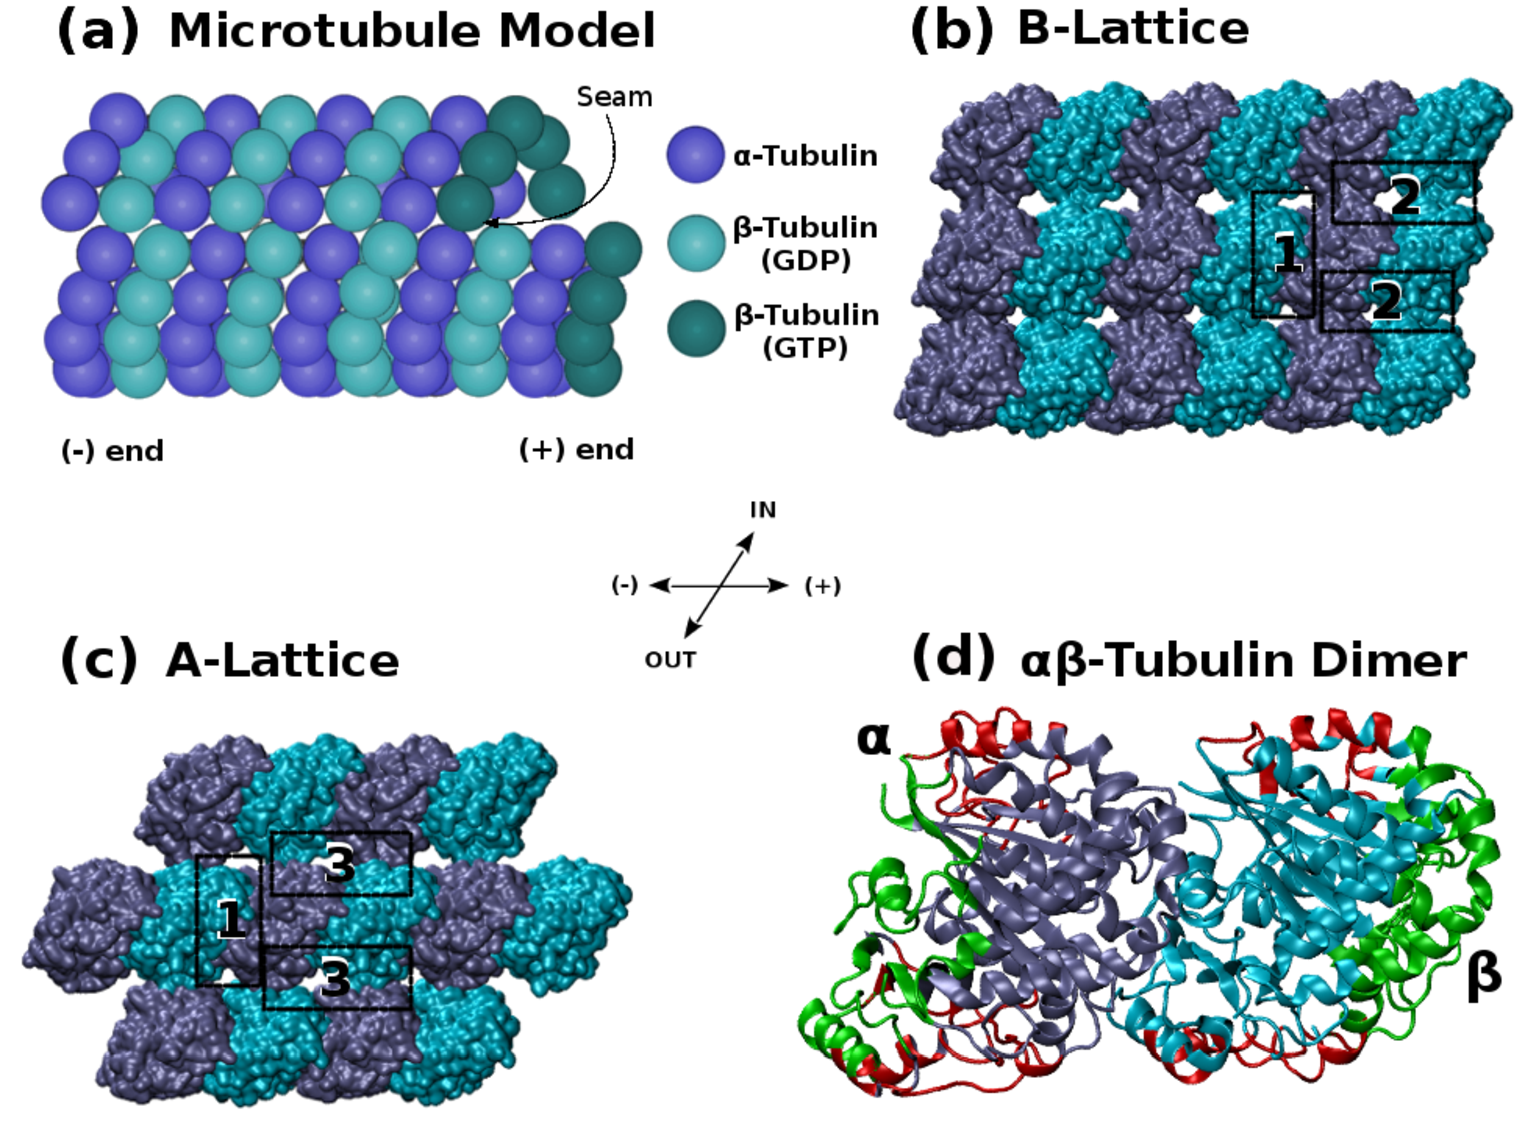
\includegraphics[width=0.8\linewidth,trim= 0.1cm 0.1cm 0.1cm 0.1cm, clip=true]{images/System.pdf}
  \caption[Microtubule lattice and interfaces]{Microtubule lattice and interfaces, with (dark blue) $\alpha$-subunits and (cyan) $\beta$-subunits. (a) A model of a microtubule cylinder. (b) A model of the B-lattice configuration showing only nine tubulin dimers. (c) A model for the A-lattice configuration showing only seven tubulin dimers. In panels b and c, the three different interfaces between tubulin dimers that we studied are highlighted. These are 1) \gls{longab}; 2) \gls{latb}; and 3) \gls{lata}. (d) A more detailed model of the $\alpha$$\beta$-tubulin heterodimer showing the domains that make lateral contacts (red) and the domains that make longitudinal contacts (green).}
  \label{f:THB-system}
\end{figure}

\subsection{Energy Calculation using AIM Approach}
\label{ss:THB-Methods_AIM}

A hydrogen bond is a bond that involves three atoms: a hydrogen atom (H) attached covalently to an electronegative atom, such as N, O, or F, as one partner and an electronegative atom as another partner. The former electronegative partner is called the \gls{hd} whereas the latter electronegative partner is called the \gls{ha}. Bader's AIM theory is a very attractive and successful method of characterizing bond strengths based on properties of critical points
\cite{Bader1990,Bader1991}. 
Several successful studies that characterized hydrogen bonds based on topological properties of electron density at the bond critical points have been reported \cite{Popelier1998,Grabowski2001,Scheiner2001,Parthasarathi2006}. In a previous study,we built a strong linear correlation between the density at the \gls{bcp} located between the hydrogen atom and the acceptor atom, $\rho_{H-A}$, and the strength of the hydrogen bond obtained from a supermolecular approach
\cite{Ayoub2014HB}. 
The relationship had a coefficient of determination, $r^2$, of 0.96. This relationship was true for all kinds of
hydrogen bonds that span the range of $0-60$ kJ/mol, as reflected by the heterogeneous training set used. Using this relationship, we obtained the parameters necessary for calculating the strength of hydrogen bonds by knowing only the value of the electron density, $\rho_{H-A}$, at the BCPs
\cite{Ayoub2014HB}. 
This relationship is given as:
\begin{equation}
\label{eq:THP-fit}
E_{\emph{HB}} = m\, \rho_{HA} + b
\end{equation}
where $E_{\emph{HB}}$ is the energy calculated from a supermolecular approach, and $m$ and $b$ is the slope and the intercept of the linear correlation obtained, respectively. The parameters $m$ and $b$ were used to calculate the strength of hydrogen bonds in the tubulin interfaces.

\subsection{Molecular Dynamics Simulations}
\label{ss:THB-Methods_MDSim}

Toward calculating the energies of hydrogen bonds in our system using this method, we obtained the Protein Data Bank (PDB)
\cite{Bernstein1978} crystal structure of bovine brain tubulin PDB:1JFF
\cite{Lowe2001} and repaired it via basic homology modeling by adding missing residues from PDB:1TUB
\cite{Nogales1998} using the software MODELER 9V6
\cite{Sali1993}. 
The repaired PDB:1JFF structure was optimized using energy minimization via a conjugate gradient method over 40,000 time steps in an MD simulation in a neutralized water box using the NAMD program
\cite{Phillips2005}. 
Using this minimized structure, the microtubule A- and B-lattice structures based on the microtubule geometry described in Li et al.
\cite{Li2002} and Sept et al.
\cite{Sept2003} were built using an in-house PYTHON script in the software PYMOL0.99rc6
\cite{PyMol} \footnote{Model building was done with the assistance of
T. Craddock, Nova Southeastern University, Florida.}. 
Lateral orientation of the B-lattice was verified by overlaying a pair of lateral tubulin heterodimers from our model to the model prepared by Wells and Aksimentiev
\cite{Wells2010}. 
A root mean-square deviation (RMSD) of only 3.4 \r{A}
was reported, which is actually smaller than the resolution of the PDB:1JFF structure itself (3.5 \r{A}).

Subsequently, a pair of interacting $\alpha$$\beta$-tubulin heterodimers were separated from each lattice to be used to study the hydrogen bonds. Specifically, a pair of longitudinal neighbors from the B-lattice model was separated to study the longitudinal interface (LongAB), a pair of lateral neighbors was separated from the B-lattice model to study the lateral B interface (LatB), and a third pair of lateral neighbors from the A-lattice was separated to study the lateral A interface (LatA). All the interfaces as well as the interacting pairs of $\alpha$$\beta$-tubulin heterodimers that were separated are shown in 
Fig. \ref{f:THB-system}. 
Hence, we investigated three distinct systems, each containing a pair of $\alpha$$\beta$-tubulin heterodimers. For each $\alpha$$\beta$-tubulin pair system, we ran an MD simulation to obtain an equilibrated system. In detail, we added the cofactors, GTP and GDP, to their binding sites with the help of SWISS PDBVIEWER 4.1
\cite{Guex1997}. 
Taxol, or any other stabilizer, was not added to the system.

As stated earlier, terminal $\beta$-subunits that are not capped with GTP are
unstable and prone to depolymerization. Therefore, the terminal $\beta$-subunits in the three systems were all capped with GTP instead of GDP. The magnesium ion at the $\alpha$-subunit GTP binding site was also included to stabilize the complex. C-termini were capped with $n$-methylamide residues. The C-terminal tails were not simulated because they are not available in PDB structures, and they are highly mobile and variable among tubulin isotypes. The C-terminal tail is also far away from lateral and longitudinal interfaces, and hence is not expected to have any direct contribution to lateral interactions. Moreover, the inclusion of this tail would require the usage of a very large water box that would significantly increase the computational load. We parameterized the protein system using the AMBERff12SB force field
\cite{Cornell1995,Hornak2006}.
We parameterized the cofactors using the parameter set developed by Meagher et al.
\cite{Meagher2003}. Ionization states were assigned using the PROPKA server
\cite{Li2005,Bas2008,Olsson2011,Sondergaard2011}. 
Each system was solvated with a TIP3P water box extending 10 \r{A}
in each direction and neutralized by the addition of 72 Na$^{+}$ ions.

Additional ion pairs of Na$^{+}$ and Cl$^{-}$ were added to bring the ion concentration to 100 mM to mimic cellular conditions. Although the initial coordinates were obtained from a 13-protofilament microtubule model, we are effectively simulating a free pair of tubulin heterodimers in each system, given the geometry of the water box used. Then, the AMBER MD package
\cite{case2012} was used to minimize the complex through a series of 2000 steepest-descent and conjugate gradient steps with strong restraints on the protein heavy atoms (500 kcal mol$^{-1}$ \r{A}$^{-2}$). 
This was intended to relieve any
hydrogen contacts caused by the addition of hydrogens using AMBER residue templates. Another 4500-step minimization was done to bring the whole system to the nearest local energy minimum. Then the system was heated, over 20 ps under constant volume, to a temperature of 310 K by the Langevin thermostat using restraints on the protein (10 kcal mol$^{-1}$ \r{A}$^{-2}$).

The restraints were then released gradually through a 100-ps run under
constant pressure and temperature, and a production phase of 30-45 ns was run under the same conditions to attain RMSD equilibration. This production step was performed using GPU cores on the PharmaMatrix Cluster (University of Alberta) through the AMBER GPU-accelerated code
\cite{Salomon-Ferrer2013,Gotz2012,LeGrand2013}. 
All simulations were performed using periodic boundary conditions where the particle-mesh Ewald method was used for treating long-range electrostatics with a cutoff of 8.0 \r{A}. When considering RMSD equilibration, we
gave more attention to the interfacial residues than the residues that are distant from the interface. We clustered the snapshots that correspond to 20 ns extracted from the equilibrated region in the trajectories based on RMSD of the interfacial residues in eight clusters, using the average linkage algorithm
\cite{Shao2007} 
through the CPPTRAJ module of AMBER \cite{Roe2013}.

The centroid of the each cluster was considered to be the most representative structure of the cluster, and was processed further. Therefore, we used eight snapshots for every system. Each snapshot was processed using the CPPTRAJ module of AMBER to detect all hydrogen bonds. This is done by AMBER by listing all possible hydrogen-bond donors (HD) and acceptors (HA) in the system and then analyzing the distances between them as well as the angle made by HA-H-HD atoms. A cutoff of 3.0 \r{A} for distance and 135$^{\circ}$
for angle are used as default criteria by AMBER for hydrogen bonds. Although these values are reasonable
\cite{Wendler2010}, 
we relaxed the strictness of our criteria to a distance of 3.3 \r{A}
and an angle of 120$^{\circ}$, and then depended on
the AIM method to confirm the presence of each hydrogen bond (a bond is present if there is a nonzero electron density at the bond critical point).

These relaxed criteria were used to prevent missing any possible hydrogen
bonds, i.e., to prevent false-negatives. The hydrogen bonds detected by AMBER were analyzed and all the bonds that are not interfacial in nature, i.e., not binding the two $\alpha$$\beta$-tubulin heterodimers together, were ignored. Other energetic contributions such as van der Waals and electrostatic interactions were also estimated using the  \gls{mmgbsa} method as implemented in AMBER
\cite{Kollman2000}. 
The program VMD 1.9.1 was used for viewing the MD trajectories
\cite{Humphrey1996}. 
After that, every hydrogen-bonding residue pair was analyzed individually using the AIM method.

\subsection{Quantum Mechanical Calculations}
\label{ss:THB-Methods_QM}

Each pair of interacting amino-acid residues was characterized in a separate QM single-point calculation. The QM region was specified as the parts of the two residues making the hydrogen-bond contact, and we avoided cutting at polar or saturated bonds. The rest of the $\alpha$$\beta$-tubulin pair system, i.e. the MM region, was treated, together with the solvent, using electronic embedding, which incorporates the partial charges of the MM region into the quantum-mechanical Hamiltonian. This technique provides a better description of the electrostatic interaction between the QM region and the MM region (because it is treated at the QM level) and allows the QM wavefunction to be polarized. Table \ref{t:THB-Cutting} lists the bonds that were cut to separate the QM region from MM region. The QM region was treated using density functional theory with the density functional B3LYP
\cite{Becke1993,Lee1988,Vosko1980} 
and the basis set TZVP
\cite{Schaeffer1992,Schaeffer1994}. 
This functional and basis set were chosen to match the ones that we used to develop the parameters
\cite{Ayoub2014HB}.

All the QM calculations were done using the software GAUSSIAN 09
\cite{g09}. Subsequently, an AIM analysis was carried out using GAUSSIAN 09 and the electron densities at the BCPs were obtained. Difficult cases, i.e., cases that did not converge in Gaussian, were treated using the software suite AIMPAC which is more stable
\cite{AIMPAC}.
The hydrogen-bond energy
was calculated using the parameters that we had developed in Ayoub et al.
\cite{Ayoub2014HB}. 
This QM calculation was applied to each instance of hydrogen bonding occurring between any pair of residues. Hence, we built several BASH scripts to automate all these procedures. As stated earlier, we used eight different representative snapshots for every system, and hence all these calculations were repeated for every snapshot. The total hydrogen-bond energies, as well as the per-residue energies, for each of the three main systems used were then obtained and analyzed.

\begin{table}
	\caption[Cutting bonds for QM/MM interface]{Cutting bonds for QM/MM interface. The table lists the bonds that were cut to separate the QM from
	the MM region for each hydrogen-bonded residue. In all side-chain hydrogen bonds, the side chain, after the cut indicated in the table, was treated with QM. In backbone hydrogen bonds, atoms C, O, N, H, CA, and HA were treated 
	with QM in all residues except Gly where the side chain was also included in the QM region. Amber atom names are used in the table (i.e. A, B, C, ... stand for $\alpha, \beta, \gamma,$ ..., respectively).}
	\label{t:THB-Cutting}
	\centering
	\begin{tabular*}{\linewidth}{@{\extracolsep{\fill}}llll}
		\toprule
		Residue & Bond cut & Residue & Bond cut\\
		\midrule
		Glu & CB--CG & ARG & CG--CD\\
		Asp & CA--CB & GLN & CB--CG\\
		Lys & CD--CE & Asn & CA--CB\\
		His & CA--CB & Thr & CA--CB\\
		Ser & CA--CB & Trp & CA--CB\\
		Tyr & CA--CB & &\\
		
		\bottomrule
	\end{tabular*} 
\end{table}


\section{Results and Discussion}
\label{s:THB-Results}

The MD simulation runs were continued until RMSD equilibration of the interfacial residues was attained (interfacial residues are residues that have at least one atom within 8 \r{A} from the neighboring tubulin heterodimer). Other residues distant from the interface were not considered, as they do not contribute to interfacial hydrogen bonding. 
Fig. \ref{f:S-THB-rmsd} in the Appendix shows the RMSD equilibration plot of the backbone atoms of interfacial residues relative to the starting structure. The LatB and LongAB systems were equilibrated early in the simulations. For LatA, we pursued the simulations a bit longer to make sure that the system was well equilibrated. The trajectory of the equilibrated region of each system was clustered in eight clusters, as explained before. These eight representative snapshots were analyzed for hydrogen bonds, and each pair of interacting residues was then subjected to a QM calculation and AIM analysis. The results of each system are listed in 
Tables \ref{t:THB-LongAB}--\ref{t:THB-LatA}.
Each table shows the average total hydrogen-bond energies as well as the average per-residue energies over the eight different representative snapshots that were processed.

It should be noted that hydrogen bonds are highly dynamic in nature, which means that they keep forming and breaking over the course of the MD simulation. Therefore, we expect to see large variations in the per-residue hydrogen-bond energies, and this is why the standard deviation (SD) can sometimes be very high. In this case, high SD would represent highly dynamic bonds, whereas low SD would represent bonds that are persistent over the course of the MD trajectory. SD, in this case, does not reflect statistical errors in the calculations; instead, it reflects the transitory nature of each individual bond. However, the total hydrogen-bond energy values are expected to have a relatively smaller SD because bonds that are broken over the course of the trajectory are usually replaced by other bonds that are forming simultaneously.


Hence, we should have more precise values for the over-
all hydrogen-bond energies. These variations could, however, be compensated for by other binding interactions, such as electrostatic interactions or van der Waals interactions, which were not included in this study. It is also important to note that the per-residue energies listed in the tables include all hydrogen-bond instances between the residue pairs. Therefore, the energy could be due to more than one hydrogen bond between the interacting pair.
The tables
only list hydrogen bonds that are stronger than $-10$ kJ/mol. Other weak bonds are included in the Appendix. Residue numbering follows the same scheme as in PDB:1JFF
\cite{Lowe2001}.

\subsection{Longitudinal Interactions}
\label{ss:THB-Results-longAB}

The longitudinal (LongAB) interface (see 
Fig. \ref{f:THB-system}b ) is particularly important as it contributes to the building of a protofilament and happens to accommodate an important class of anticancer agents. This class includes the microtubule destabilizers known as vinca alkaloids
\cite{Gigant2005,Toso1993}. 
Understanding the interactions at this interface could give us insight into the mechanism of action for vinca alkaloids. An all-atom model of the LongAB system with subunit assignment can be found in 
Fig. \ref{f:S-THB-LongAB}. 
Analyzing the results for the LongAB interface listed in 
Table \ref{t:THB-LongAB}, 
we find that the total hydrogen-bond energy is $-392\pm59$ kJ/mol. The table also shows the per-residue hydrogen-bond energies between the $\alpha$-subunit of heterodimer 1 and the $\beta$-subunit of heterodimer 2. As shown in this table, the strongest bond network is the one between $\alpha$Arg2 and $\beta$Glu71 with an average energy of $-40.1$ kJ/mol. This bond is also persistent along the MD trajectory, as shown by the relatively low SD. $\alpha$Arg2 is, in fact, the very first residue in tubulin after the first methionine, and it makes an energetically significant bond. The second partner of this strong bond, $\beta$Glu71, is present in the S2-H2 loop of the $\beta$-tubulin, which shows the importance of this loop to longitudinal stability. 

Another important residue is $\beta$Arg401, which is present in
the H11-H11' loop. This residue alone makes several strong hydrogen-bond networks with $\alpha$Glu434 ($-32.6$ kJ/mol), $\alpha$Tyr262 ($-32.1$ kJ/mol), and $\alpha$Asp438 ($-23.9$ kJ/mol), summing up to a total of nearly $-90$ kJ/mol on average, which
\begin{table}
  \caption[Energy of hydrogen bonds in the LongAB interface]{Energy of hydrogen bonds in the LongAB interface. 
  This structure refers to two $\alpha\beta$--tubulin 
  heterodimers aligned longitudinally (TUB 1 and TUB 2). 
  Average energy and standard deviation (SD) values are taken from eight
  different representative snapshots.
  Energies are expressed in kJ/mol.}
  \label{t:THB-LongAB}
  \centering
  \begin{tabular*}{\linewidth}{@{\extracolsep{\fill}}llcc}
    \toprule
    TUB 1--$\alpha$&	TUB 2--$\beta$	&	$E_{\text{average}}$	&	SD	\\
    \midrule
    Arg2	&	  Glu71		&	--40.1	&	14	\\
    Glu434	&	  Arg401	&	--32.6	&	17	\\
    Tyr262	&	  Arg401	&	--32.1	&	17	\\
    Arg243	&	  Asp76	        &	--29.9	&	14	\\
    Thr349	&	  Val181	&	--25.8	&	12	\\
    Asp438	&	  Arg401	&	--23.9	&	25	\\
    Val260	&	  His406	&	--22.1	&	11	\\
    Gln133	&	  Gly98	        &	--21.9	&	8	\\
    Thr257	&	  Gly100	&	--21.4	&	7	\\
    Lys352	&	  Thr180	&	--18.7	&	9	\\
    Asn249	&	  Gln11	 	&	--18.6	&	11	\\
    Asn329	&	  Lys176	&	--15.3	&	10	\\
    Lys163	&	  Glu411	&	--14.7	&	19	\\
    Asn258	&	  Val181	&	--13.9	&	8	\\
    \multicolumn{2}{l}{Other Bonds}&--61.3&---\\
    \multicolumn{2}{l}{Total Energy}&--392&59\\
    \bottomrule
  \end{tabular*} 
\end{table}
is nearly one-fourth of the total binding energy. Thus, residue $\beta$Arg401 could be described as the longitudinal glue of microtubules. Two of the partners that bind to this residue, namely $\alpha$Glu434 and $\alpha$Asp438, belong to the C-terminal tail of the $\alpha$-subunit. Residues from 176 to 181 in $\beta$-tubulin, which correspond to the S5-H5 loop, make several hydrogen-bond networks with $\alpha$-residues that belong to helix H10 through loop S9-S10. These bonds collectively make up nearly $-90$ kJ/mol, which comprises nearly one-fourth of the overall stability, and again reflects the importance of the S5-H5 loop in longitudinal stability.

The bonds involving S5-H5 loop are not only collectively
strong, but they are also relatively persistent during the MD simulation, as indicated by their relatively low SD values. In fact, it has been shown that the S5-H5 loop in $\beta$-tubulin, particularly residues from 174 to 179, are very important for the vinca alkaloid binding and they comprise part of the vinca binding site
\cite{Gigant2005,Torin2006}. Considering that, as shown in this work, the same region contributes significantly to the longitudinal stability indicates that it is very likely that the binding of these anticancer agents destabilizes microtubules simply by disrupting the longitudinal hydrogen-bond networks between adjacent heterodimers along a protofilament. This could be verified by performing another equivalent study in the presence of one of these agents, then comparing the results.

The bonds made by $\beta$Gly100 and $\beta$Gly98 on one side and
$\alpha$Thr257 and $\alpha$Gln133 on the other side, respectively, are also strong and steady with relatively low SD, suggesting a strong and persistent stabilization due to the S3-H3' loop of $\beta$-tubulin. It is also noticeable that GDP has no contribution to longitudinal stability when hydrogen bonds are considered; it does not appear in our list, although it binds close to the longitudinal interface. It is worth mentioning that residues making hydrogen-bond networks with more than one residue, such as $\beta$Arg401, usually have a relatively high SD. This is not surprising because during the MD simulation, such a residue may break its bonds with one residue and soon form other bonds with another residue to maintain the longitudinal stability. This behavior raises the SD calculated over the eight representative snapshots for each bond. All the major hydrogen bonds in the longitudinal interface are shown in Fig.
\ref{f:THB-longHB}. 
It is obvious that major strong hydrogen bonds are well distributed along the width and the length of the longitudinal interface, which imparts even more stability to the protofilaments because they act as pillars for the protofilament structure. Residue $\beta$Arg401 and its strong and persistent hydrogen-bond network are also shown in the figure.

\subsection{Lateral B Interactions}
\label{ss:THB-Results-LatB}

The LatB interface represents the lateral interface between two tubulin dimers in two adjacent protofilaments in the B-configuration (see Fig.
\ref{f:THB-system}b). An all-atom model of the
LatB system with subunit assignment can be found in Fig.
\ref{f:S-THB-LatB}. This interface is especially important not only because it brings protofilaments together to form a microtubule cylinder, but because it is also very close to the taxane binding site. The taxane binding site is the binding site for many microtubule-stabilizing antimitotic drugs such as taxol, epothilone, discodermolide, eleutherobin, and sarcodictyin
\cite{Bollag1995,Hamel1999,Kowalski1997,Buey2005,Ayoub2014}. Analyzing the lateral interface could give us an insight into the detailed mechanism of action of such agents. The first and most obvious observation in Table
\ref{t:THB-LatB} 
is that, in a 95\% confidence interval, lateral hydrogen bonds are significantly stronger than longitudinal ones, $-462\pm70$ vs. $-392\pm59$ kJ/mol.

\begin{figure}
  \centering
  \caption[Major hydrogen bonds at the longitudinal interface]{Major hydrogen bonds at the longitudinal interface.
  It is clear that they are distributed all over the width and length
  of the interface to provide stronger support to the protofilament
  structure.}
  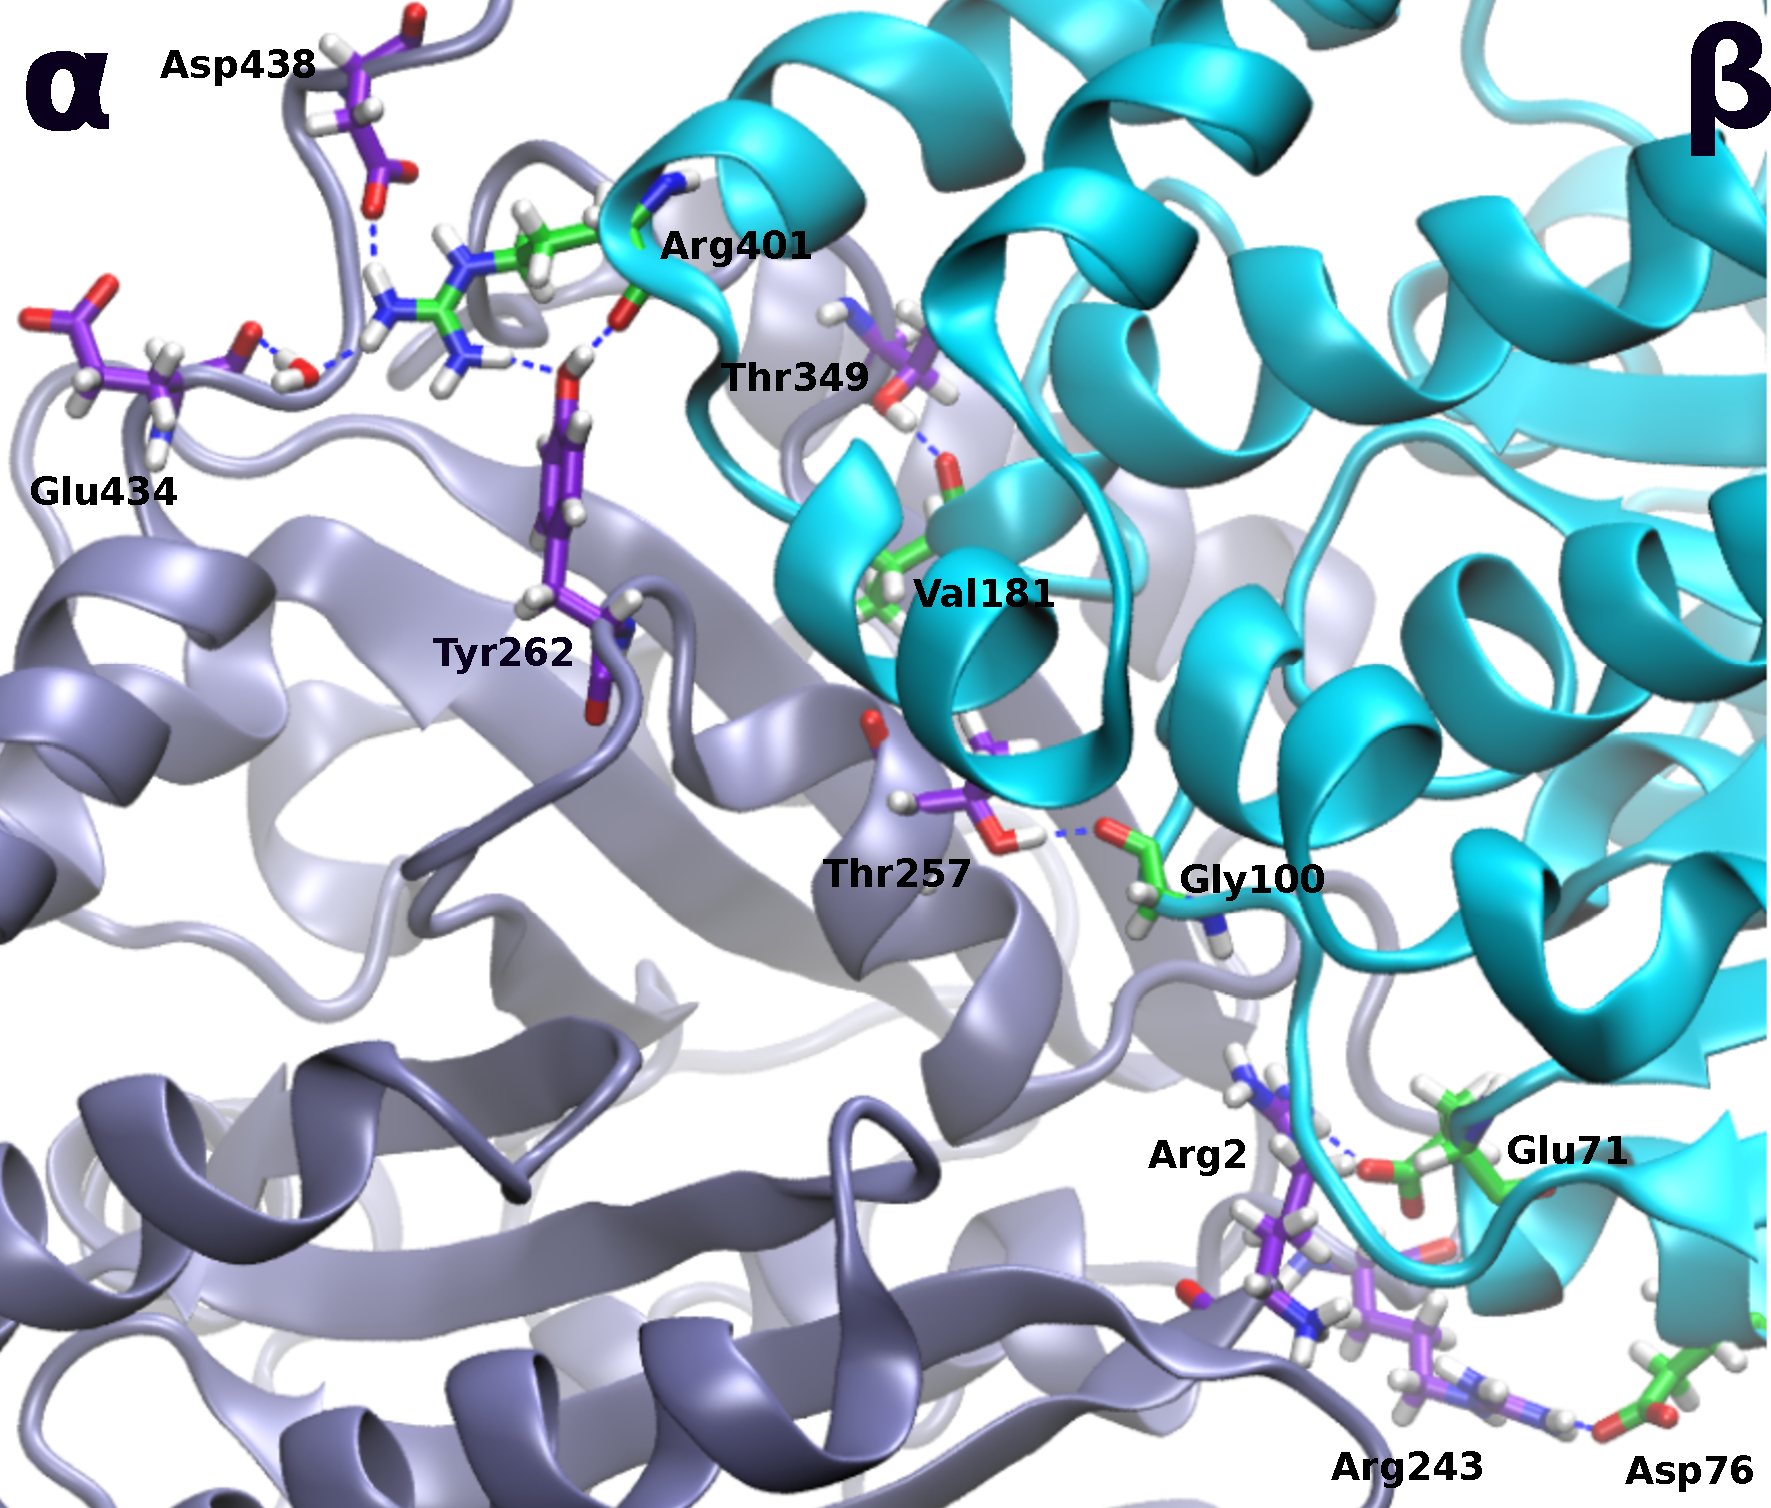
\includegraphics[width=0.7\linewidth]{images/HB-LongAB}
  \label{f:THB-longHB}
\end{figure}

This is apparently counterintuitive, because we know, a
priori, that lateral contacts break before longitudinal ones and this is why depolymerizing microtubules display transient structures that look like ram's horns
\cite{Sept2003,VanBuren2002}. 
There could be two justifications for getting such results: the first one is that we only calculated the respective hydrogen-bond energies. Other sources of energies could balance out this energy difference. Particularly, electrostatic interactions and dipole-dipole interactions are expected to be more destabilizing in the lateral orientation than in the longitudinal one. This is because the similarly-charged subunits are packed closer together in the lateral orientation than in the extended longitudinal one. 
We estimated the van der Waals as well as electrostatic contributions using the MM/GBSA calculation and found that the longitudinal interactions in a protofilament are $\sim$ 130 kJ/mol stronger than lateral interactions, which supports our justification.

\begin{table}
  \caption[Energy of hydrogen bonds in the LatB interface]{Energy of hydrogen bonds in the LatB interface. 
  This structure refers to two $\alpha\beta$--tubulin 
  heterodimers (TUB 1 and TUB 2) aligned laterally in the 
  B--configuration. 
  Average energy and standard deviation (SD) values are taken from eight
  different representative snapshots.
  Energies are expressed in kJ/mol.}
  \label{t:THB-LatB}
  \centering
  \begin{tabular*}{\linewidth}{@{\extracolsep{\fill}}llccccllcc}
    \toprule
    \multicolumn{4}{c}{\textbf{$\alpha$--$\alpha$ Interactions}}&&&\multicolumn{4}{c}{\textbf{$\beta$--$\beta$ Interactions}}\\
    \cmidrule(r){1-4} \cmidrule(l){7-10}
    TUB 1--$\alpha$&TUB 2--$\alpha$&$E_{\text{average}}$&SD&&&TUB 1--$\beta$&TUB 2--$\beta$&$E_{\text{average}}$&SD\\
    \midrule
    Arg215&  Glu90&--42.7&18&&&Arg308&  Asp116&--44.8&20\\
    Lys338&  Asp127&--28.5&8&&&Glu290&  Arg88&--38.9&12\\
    Glu297&  Arg121&--24.6&19&&&Arg308&  Asp120&--36.7&14\\
    Glu297&  Lys124&--23.6&12&&&Lys299&  Asp90&--32.6&12\\
    Glu284&  Ser54&--22.3&14&&&Asp297&  Lys124&--22.3&19\\
    Gln372&  Glu55&--18.4&9&&&Tyr342&  Asp120&--18.4&18\\
    Tyr282&  Ser48&--11.7&11&&&Ser280&  Arg88&--16.6&16\\
    His283&  Phe49&--10.5&8&&&Lys338&  Lys124&--14.8&10\\
    &&&&&&Lys338&  Ser126&--12.0&11\\
    \multicolumn{2}{l}{{Other Bonds}}&--27.5&---&&&\multicolumn{2}{l}{{Other Bonds}}&--14.8&---\\
    \multicolumn{2}{l}{Subunit Energy}&--210&35&&&\multicolumn{2}{l}{Subunit Energy}&--252&65\\
    \multicolumn{8}{l}{Total Energy}&--462&70\\
    \bottomrule
  \end{tabular*} 
\end{table}

The other possible reason for this difference is that in the LatB simulations we actually modeled GTP-capped tubulin dimers, as explained in Methods.
Terminal tubulin dimers capped with GTP stabilize
microtubule structures more strongly than those capped with GDP, which is why depolymerization usually happens after hydrolysis of the terminal GTP
\cite{Mitchison1984}. 
Hence, lateral contacts in our case are expected to be enhanced by the presence of GTP, and this could be the reason why they are stronger than longitudinal ones. Preliminary results from other simulations being presently performed support this explanation, because we found out that in the presence of GDP instead of GTP, the two heterodimers are significantly more weakly connected to one another. 
The data in Table
\ref{t:THB-LatB} 
also show that the average contribution of the $\beta$-$\beta$ interactions is comparable to the average contribution of the $\alpha$-$\alpha$ interactions, namely $-252\pm65$ vs. $-210\pm35$ kJ/mol, at a 95\% the confidence interval. However, if the simulations were run in presence of taxol, the relative contributions of the two subunits could have been different.

Examining the $\beta$-$\beta$ subunit interactions, we find out that
the strongest hydrogen-bond network is the one between $\beta$Arg308 (from the H9' helix) and $\beta$Asp116, with a strength of $-44.8$ kJ/mol and a relatively moderate SD, signifying persistence of the bonds over the MD trajectory. $\beta$Arg308 still makes another strong and largely persistent bond with $\beta$Asp120, at a strength of $-36.7$ kJ/mol. Thus, $\beta$Arg308 contributes, in total, nearly $-80$ kJ/mol to lateral stability, which is nearly one-third of the overall $\beta$-$\beta$ stabilization. $\beta$Glu290 and $\beta$Arg88 contribute a largely persistent hydrogen-bond network of $-38.9$ kJ/mol. The H2-S3 loop, which involves $\beta$Arg88 and $\beta$Asp90, is extensively involved in lateral stabilization, making bonds that sum up to nearly $-90$ kJ/mol, which is nearly one-third of the overall $\beta$-$\beta$ hydrogen- bond energy. The H3 helix, which involves residues $\beta$Asp116, $\beta$Asp120, $\beta$Lys124, and $\beta$Ser126 and others, is responsible for most of the stabilization occurring between $\beta$-subunits. Interactions involving these residues sum up
to a total of nearly $-165$ kJ/mol, which is approximately two-thirds of the overall $\beta$-$\beta$ stabilization.

Thus, H2-S3 loop is responsible for one-third of $\beta$-$\beta$
hydrogen-bond energy, and the H3 helix is responsible for the remaining two-thirds. On the other hand, the contribution of the M-loop from the opposite $\beta$-subunit (TUB 1-$\beta$ in Table
\ref{t:THB-LatB}) is relatively small compared to the H3 helix contribution from TUB 2-$\beta$, amounting to only $-16.6$ kJ/mol on average, via bonds that involve $\beta$Ser280 from the M-loop. 
The H1-S2 loop in TUB 2-$\beta$ has no contribution to lateral hydrogen-bonding in B-lattice. This is contrary to the conclusions that were drawn by Li et al.
\cite{Li2002}, 
who argued that lateral stability is mostly due to interactions between M-loop and H1-S2 loop rather than being due to the H3 helix.
\begin{figure}
  \centering
  \caption[Relative orientation of the two adjacent heterodimers]{Relative orientation of the two adjacent heterodimers in the LatB
  system before the simulation (orange) and after 25 ns of the simulation (cyan).}
  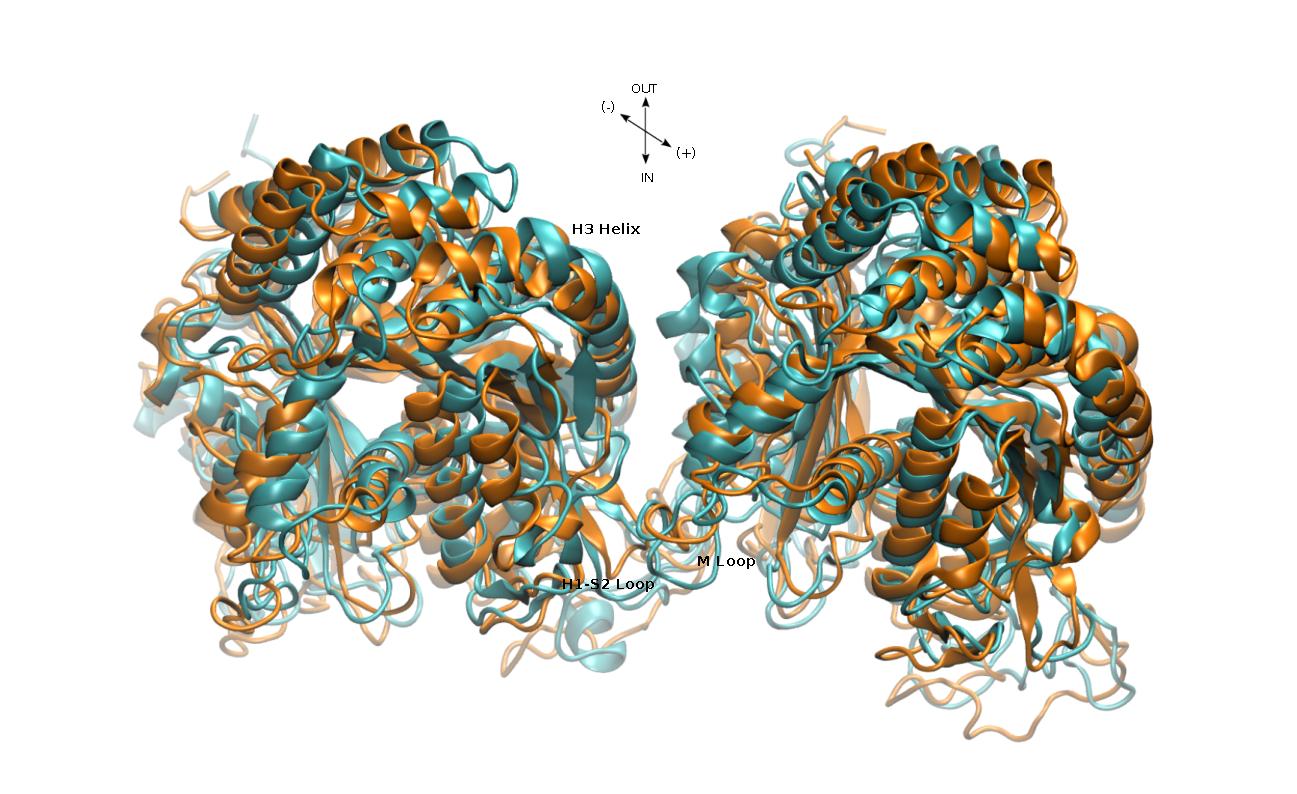
\includegraphics[trim= 2.3cm 0.8cm 2.3cm 1.3cm, clip=true, width=0.9\linewidth]{images/H3-rot}
  \label{f:THB-H3-rot}
\end{figure}
 However, these authors stated that this result itself is contrary to a previous conclusion they reached, which attributed most of the lateral stability to the H3 helix rather than the H1-S2 loop. This shows some discrepancies that could be attributed to the fact that their conclusions were not based on a study of the energetics of lateral contacts, but only on geometric criteria. It could also be attributed to the fact that we considered hydrogen bonds only, in this study. Other energetic components could still come into play.
However, considering the conditions of our simulations,
the difference between the results of Li et al.
\cite{Li2002} 
and our findings may be understood because microtubules stabilized by taxol were used in their experiments but not in ours.
 It is known that taxol restructures the M-loop in a way that stabilizes lateral contacts \cite{Li2002,Nogales1999,Snyder2001,Amos1999}. Because our simulations did not include taxol or any other stabilizer, we do not expect our results to match the results of Li et al.
\cite{Li2002} with regards to the role of the M-loop in imparting lateral stability. Moreover, Li et al. argued that the role of the H3 helix becomes more pronounced when the number of protofilaments in a microtubule increases, inasmuch as this decreases the angle between laterally adjacent protofilaments and brings the H3 helix closer to the neighboring heterodimer. This could be more similar to our simulated system that included only one pair of heterodimers instead of a complete microtubule, and thus could rearrange during the course of the MD simulations and draw the subunits closer to generate more H3 helix contacts. 
Fig. \ref{f:THB-H3-rot}
shows the LatB system before (orange) and after (cyan) the simulations.
It is clear that after the simulations, the two heterodimers
have rotated inward, coming closer to each other and creating more interactions with the H3 helix at the expense of breaking interactions between the M-loop and the H1-S2 loop. 

\begin{figure}
  \centering
  \caption[Major hydrogen bonds in the LatB system]{Major hydrogen bonds in the LatB system
  at (a) $\beta$--$\beta$ interface and (b) $\alpha$--$\alpha$ interface.}
  \subfloat[]{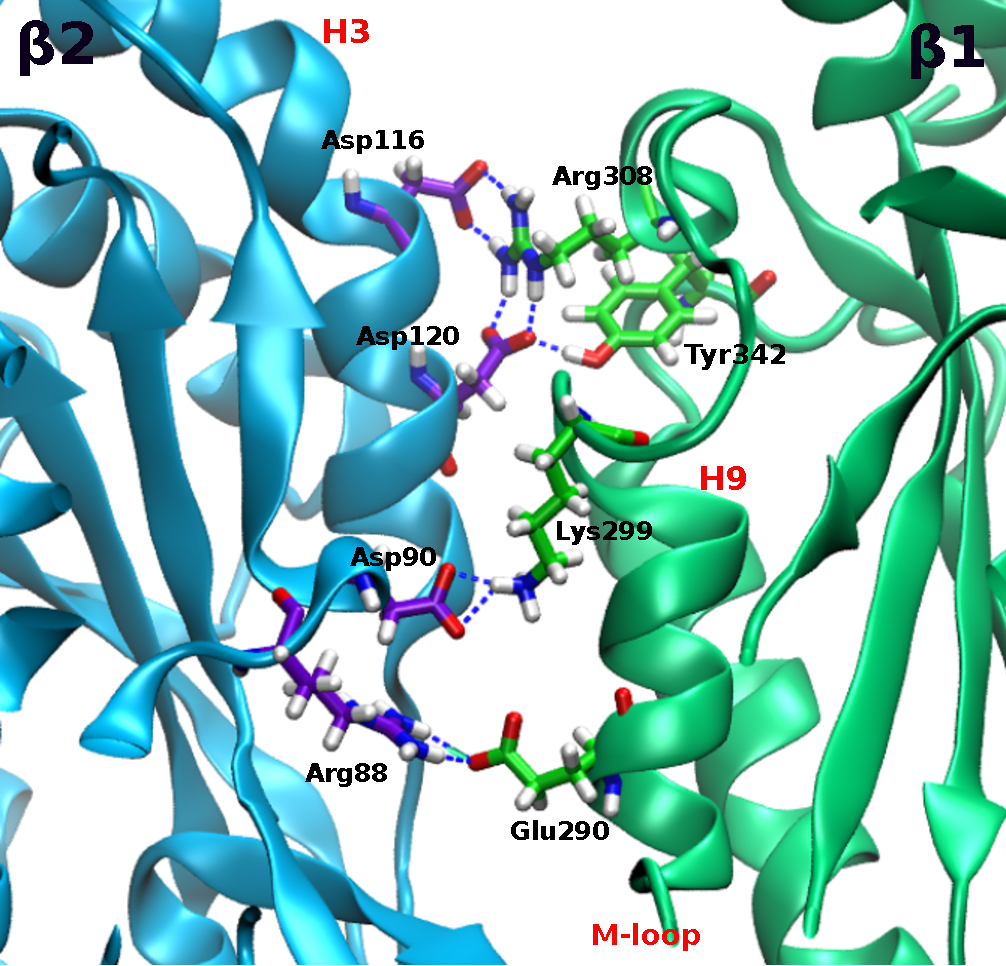
\includegraphics[width=0.465\linewidth]{images/beta-beta}}
  \hspace{0.05\linewidth}
  \subfloat[]{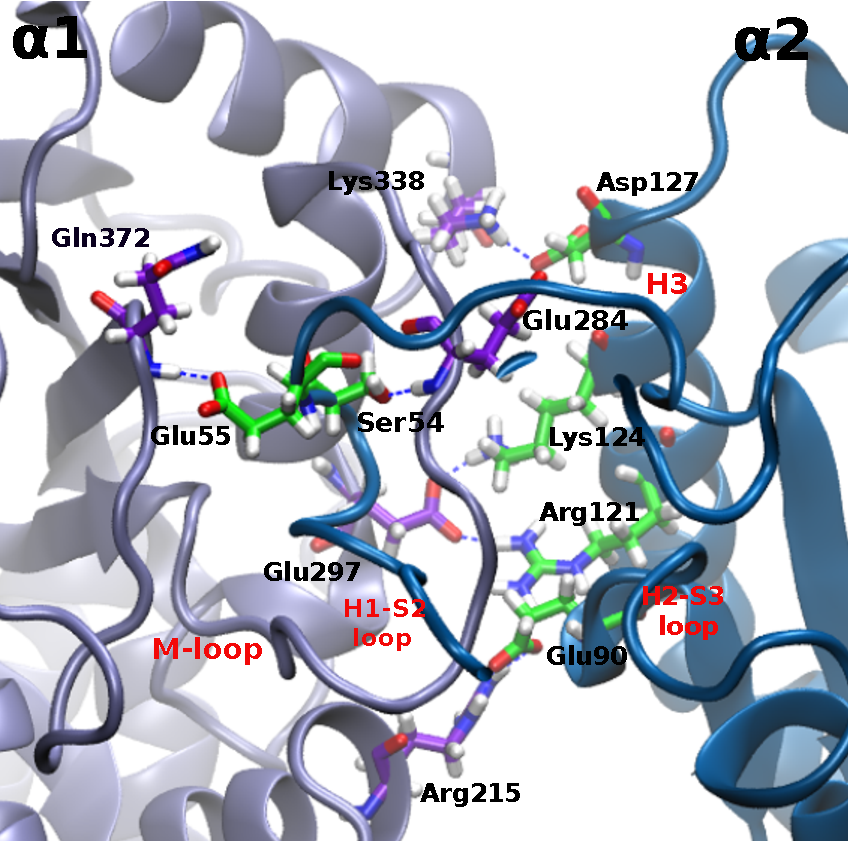
\includegraphics[width=0.45\linewidth]{images/alpha-alpha}}
  \label{f:THB-latB}
\end{figure}
Comparing the residues on our list to the residues that compose the taxol-binding site, we find that residues $\beta$Glu290 and $\beta$Ser280 are in common. These two residues make hydrogen-bond networks with the neighboring $\beta$-tubulin subunit that sum up to $-55.5$ kJ/mol, most of which comes from the bonds between $\beta$Glu290 and
$\beta$Arg88, which alone make up $-38.9$ kJ/mol. 
Comparing the role of H3 and the M-loop in lateral stability in our study and considering the finding that H3 is much more involved in stabilization than the M-loop, it appears more likely that the binding of taxol may make the M-loop more involved in lateral stability. Addition of taxol could rearrange this domain and favor stronger lateral contacts. (This could be verified by performing another simulation in the presence of taxol and estimating the per-residue contribution of all these residues.) It is worth mentioning that a conformational change of the M-loop into a short helix upon binding of stabilizers was recently confirmed by Prota et al.
\cite{Prota2013}. 
However, they did not address the energetic effects of this restructuring on lateral contacts. 
The major hydrogen-bond networks in $\beta$-$\beta$ interactions are shown in Fig.
\ref{f:THB-latB}a.

The $\alpha$-$\alpha$ interactions are similar to the $\beta$-$\beta$ ones in that
they extensively involve helix H3, with the H2-S3 loop on one side and the H9-S8 loop on the other side. However,
the
$\alpha$-$\alpha$ interactions are different because they also extensively involve interactions between the H1-S2 loop and the M-loop. These interactions involve the bonds between $\alpha$Ser54, $\alpha$Ser48, and $\alpha$Phe49 on one side and $\alpha$Glu284, $\alpha$Tyr282, and $\alpha$His283 on the other side. These, and other bonds between the M-loop and the H1-S2 loop shown in Table
\ref{t:S-THB-LatB}
in the Appendix, add up to an average total of nearly $-63$ kJ/mol. It is also apparent that the hydrogen-bond network between $\alpha$Arg215 and $\alpha$Glu90 is the strongest in the system, with an average energy of $-42.7$ kJ/mol. Fig.
\ref{f:THB-latB}b shows the major hydrogen-bond networks that bring $\alpha$-subunits together in lateral orientation. An interesting phenomenon that is noticed from the figure is the intertwining of the M-loop and the N-terminal H1-S2 loop. This structure was conserved over the entire length of the MD simulation, which reflects its stability. 

The lateral interface is highly populated with oppositely charged residues as compared to the longitudinal interface; hence, we also
expect a stabilizing electrostatic contribution between these charged residues.

\subsection{Lateral A Interactions}
\label{ss:THB-LatA}

This LatA interface represents the lateral interface between protofilaments in an A-lattice configuration, shown in Fig. 
\ref{f:THB-system}c. An all-atom model of the LatA system with subunit assignment can be found in Fig.
\ref{f:S-THB-LatA}. 
The A-lattice configuration is less significant than the B-lattice because the latter has been empirically observed to be much more predominant. It is worth mentioning that to simulate an A-lattice, three, rather than two, tubulin dimers must be included in the simulation because of the subunit offset. Because this is computationally very demanding, we simulated the relevant subunits only. That is, we used $\alpha$- and $\beta$-subunits from dimer 1, a $\beta$-subunit from dimer 2, and an $\alpha$-subunit from dimer 3, discarding the $\alpha$-subunit of dimer 2 and the $\beta$-subunit of dimer 3. This is acceptable because, as illustrated in Fig.
\ref{f:THB-system}c, 
the discarded subunits have no contacts with the studied interfaces and are far away from them.

Table \ref{t:THB-LatA} 
lists the hydrogen-bond energies obtained from
the simulations. It shows that, in a 95\% confidence interval, the average overall hydrogen-bonding in the A-lattice is not significantly different from the B-lattice, with energies of $-472\pm46$ vs. $-462\pm70$ kJ/mol, respectively. Sept et al.
\cite{Sept2003} also studied the difference between B-lattice and A-lattice energetics considering solvation energy only, but they found that the B-configuration, corresponding to a subunit rise of 8-9 \r{A}, is more stable than the A-configuration,
corresponding to a subunit rise of 52 \r{A}. 
Drabik et al.
\cite{Drabik2007}
also found a similar effect when comparing the potential of mean force in the two configurations. Therefore, in light of our findings, the difference in stability between B-lattice and A-lattice configurations could be attributed to solvation energy and other energetic components rather than to hydrogen bonds. It is worth mentioning that the A-lattice configuration is not exclusive to the A-lattice; it is also a part of the B-lattice that appears only at the seam, as depicted in Fig.
\ref{f:THB-system}a.

In Table 
\ref{t:THB-LatA}, 
we differentiate between $\alpha$-$\beta$ interactions and
$\beta$-$\alpha$ interactions, because, due to differences between $\alpha$- and $\beta$-subunits, they are not identical. In our notation, $\alpha$-$\beta$ interactions represent the half of the system in which the N-terminal H1-S2 loop, helix H3, and the H2-S3 loop of the $\alpha$-subunit interact with the M-loop and other domains of the $\beta$-subunit. However, $\beta$-$\alpha$ interactions represent the other half of the system in which the opposite is true. An interesting observation is that $\beta$-$\alpha$ interactions are much stronger than $\beta$-$\alpha$ interactions, as manifested by an energy value of $-299 \pm23$ vs. $-173\pm44$ kJ/mol, respectively. 
This suggests that the involvement of the M-loop of the $\beta$-subunit, rather than the $\alpha$-subunit, in lateral contacts greatly enhances the stability of the system by interacting with N-terminal H1-S2 loop of the opposite subunit.

\begin{table}
  \caption[Energy of hydrogen bonds in the LatA interface]{Energy of hydrogen bonds in the LatA interface. 
  This structure refers to one $\alpha\beta$--tubulin 
  heterodimer (TUB 1) aligned laterally in the A--configuration
  with an $\alpha$- and $\beta$-subunit (TUB 2$\beta$ and 
  TUB 3$\alpha$). 
  Energies are expressed in kJ/mol.}
  \label{t:THB-LatA}
  \centering
  \begin{tabular*}{\linewidth}{@{\extracolsep{\fill}}llccccllcc}
    \toprule
    \multicolumn{4}{c}{\textbf{$\alpha$--$\beta$ Interactions}}&&&\multicolumn{4}{c}{\textbf{$\beta$--$\alpha$ Interactions}}\\
    \cmidrule(r){1-4} \cmidrule(l){7-10}
    TUB 1--$\alpha$&TUB 2--$\beta$&$E_{\text{average}}$&SD&&&TUB 1--$\beta$&TUB 3--$\alpha$&$E_{\text{average}}$&SD\\
    \midrule
    Asp47	&	  Arg284	&	--42.2	&	15	&&&	Arg88	&	  Glu279	&	--35.2	&	15	\\
    Lys124	&	  Asp297	&	--31.7	&	9	&&&	Lys124	&	  Glu284	&	--27.0	&	12	\\
    Gln85	&	  Ser280	&	--23.6	&	10	&&&	Ile86	&	  Tyr282	&	--23.0	&	12	\\
    Asp46	&	  Arg278	&	--23.0	&	13	&&&	Asp90	&	  Lys280	&	--18.6	&	15	\\
    Asp127	&	  Asn334	&	--22.6	&	5	&&&	Asn54	&	  Glu284	&	--14.4	&	13	\\
    Asp120	&	  Lys338	&	--22.4	&	14	&&&	Glu127	&	  Thr334	&	--13.8	&	18	\\
    Gln128	&	  Gln293	&	--18.6	&	12	&&&	Asp90	&	  Ala281	&	--12.9	&	11	\\
    Asp47	&	  Gln282	&	--16.5	&	14	&&&	Glu127  &         Thr337        &       -10.3   &	14      \\
    Glu55	&	  Arg284	&	--14.8	&	18	&&&     \\
    Arg121	&	  Asp297	&	--13.1	&	24	&&&&&&	\\
    Asp47	&	  Arg278	&	--11.9	&	13	&&&&&&	\\
    \multicolumn{2}{l}{{Other Bonds}}&--58.2&---&&&\multicolumn{2}{l}{{Other Bonds}}&--17.8&---\\
    %Need to fix Subunit total and stdev energy
    \multicolumn{2}{l}{Subunit Energy}&--299&23&&&\multicolumn{2}{l}{Subunit Energy}&--173&44\\
    \multicolumn{8}{l}{Total Energy}&--472&46\\
    \bottomrule
  \end{tabular*} 
\end{table}

In particular, residues $\beta$Arg284, $\beta$Arg278, and $\beta$Gln282 and
others make lateral hydrogen bonds with the N-terminal loop of the adjacent $\alpha$-subunit that add up to nearly $-120$ kJ/mol. Most of these bonds are absent in the $\beta$-$\alpha$ interaction half-system, and the contribution of M-loop H1-S2 loop interactions is nearly $-30$ kJ/mol. The M-loop of the $\beta$-$\alpha$ interaction half-system prefers to bind with H2-S3 loop and H3 helix. This is illustrated in Fig. \ref{f:THB-latA} a and b, which shows the major hydrogen bonds in the two half-systems. Based on this we can also expect taxol, which is hypothesized to induce M-loop lateral interactions, to impart stability to the system via this mechanism. This can even be extrapolated to the B-lattice because 
Table \ref{t:THB-LatB} 
does not record any major contribution of the $\beta$ M-loop, especially residue $\beta$Arg284, to the overall stability. Inclusion of taxol in the simulation could alter this behavior and enhance the role of the M-loop.
\begin{figure}
  \centering
  \caption[Major hydrogen bonds in the LatA system]{Major hydrogen bonds in the latA system at (a) $\alpha$--$\beta$ interface
    and (b) $\beta$--$\alpha$ interface.}
  \subfloat[]{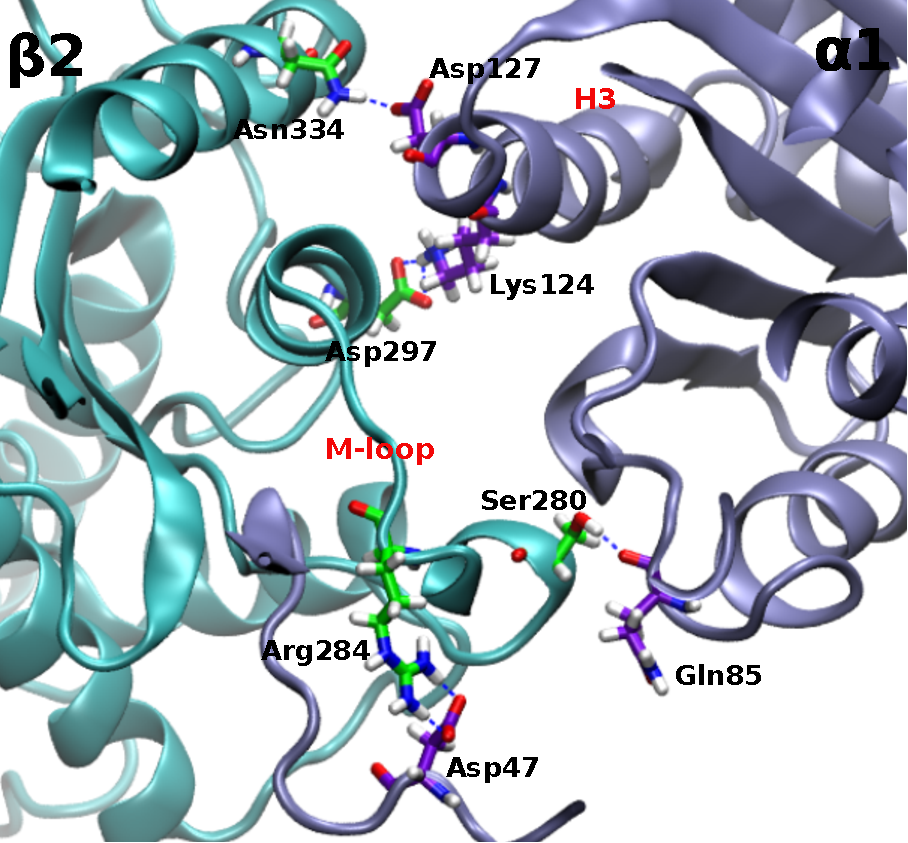
\includegraphics[width=0.45\linewidth]{images/alpha-beta}}
  \hspace{0.05\linewidth}
  \subfloat[]{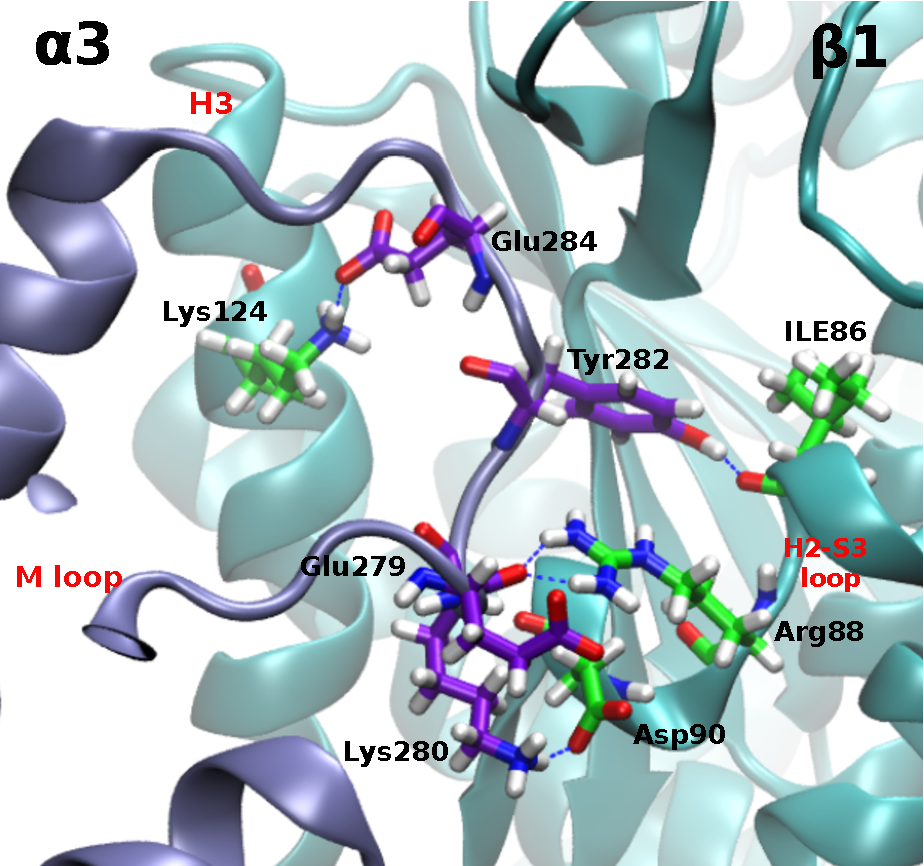
\includegraphics[width=0.45\linewidth]{images/beta-alpha}}
  \label{f:THB-latA}
\end{figure}

Finally, the comparison of the top-ranking residue pairs in
Tables \ref{t:THB-LongAB} to \ref{t:THB-LatA} to the residues that are conserved throughout different $\alpha$$\beta$-tubulin isotypes
\cite{Torin2006,Sirajuddin2014} 
showed that there is considerable agreement. In other words, residues important for interfacial stability are highly conserved among different tubulin isotypes.

\section{Conclusion}
\label{s:THB-Conclusion}

The concept of the density at the bond critical point obtained from the AIM analysis is very useful in the calculation of hydrogen-bond energies. In this article, we have implemented a seemingly new technique for the application of this method to macromolecules, namely tubulin dimer-dimer systems. The systems were equilibrated by MD simulations and then studied by QM calculations employing density functional theory followed by an AIM analysis. The three different interfaces studied, longitudinal interface
as well as lateral interfaces in B- and A-lattice configurations, revealed that hydrogen bonding is an important player in the stability of tubulin systems. One limitation of this study is the fact that we used only eight representative snapshots from the trajectory of every system. Running relatively long simulations, ensuring clustering of the trajectories, and choosing the centroid of each cluster, should alleviate this limitation. Analyzing the overall hydrogen-bond energies in different interfaces showed that lateral contacts are stronger than longitudinal ones, which was attributed to the stabilization imparted by the GTP cap on $\beta$-tubulin subunits.

The contribution of the $\beta$-$\beta$ interactions to the overall
lateral stability in the B-configuration was shown to be comparable to that of the $\alpha$-$\alpha$ interactions in a 95\% confidence interval. Running the same simulations in the presence of taxol could give different results and offer more insight into this aspect. The study also showed that the stability of the B-lattice configuration is comparable to the A-lattice when hydrogen bonds are concerned. This suggests that other energetic contributions could be responsible for the observed difference in predominance between the two lattice forms. Per-residue hydrogen-bond analysis was found to be in agreement with empirical data regarding residues critical to longitudinal stability and residues involved in the binding of vinca alkaloids. This suggests the mechanism of action of vinca alkaloids could be in the alteration of the conformations of interfacial residues upon binding, which disrupts the interfacial hydrogen-bond network and destabilizes the microtubule.

The $\beta$ M-loop was shown to have a weak contribution to
the stability of the LatB system, contrary to its large contribution to the stability of the LatA system. The weak contribution of the M-loop to the stability of the LatB system was attributed to the absence of taxol or any other microtubule stabilizer in our simulation that causes the M-loop to drift away and be replaced by helix H9 and the H9-S8 loop interacting with helix H3 in lateral contacts. Further elucidation of the role of anticancer agents would require running the
simulations in the presence of vinca alkaloids, taxol, and GDP to reach a final conclusion regarding the mechanisms of stabilization or destabilization of microtubules. Most of the residues that contributed significantly to stability of tubulin-tubulin interactions were also found to be highly conserved among different tubulin isotypes.


\chapter{Detailed Per-residue Energetic Analysis Explains the
Driving force for Microtubule Disassembly}
\label{ligHB}

\footnote{A version of this chapter was 
published as: A. T. Ayoub, M. Klobukowski, J. Tuszynski,
``Detailed Per-residue Energetic Analysis Explains the Driving Force for Microtubule Disassembly,'' \emph{PLOS Comput. Biol.}, vol. 11, issue 6, e1004313, 2015.}

\section{Introduction}

Microtubules (MTs) are cellular organelles that participate in major cellular processes such as mitosis, cell shape maintenance, cell motility and motor protein transport and constitute a major target for a wide range of drugs, most notably anti-mitotic chemotherapy agents such as paclitaxel.
Due to their importance in cell biology, MTs
have been the topic of active research into their structure and function for several decades \cite{Hyams1993}.
The pivotal role of MTs in 
cell division, by forming the mitotic spindle that segregates chromosomes, makes them an important target for antimitotic cancer chemotherapy drugs \cite{Hayden1990,Dumontet2010}. A detailed description of the MT structure
and dynamics instability was presented in Sec. \ref{MT-Intro}.

\begin{figure*}[h]
  \centering
  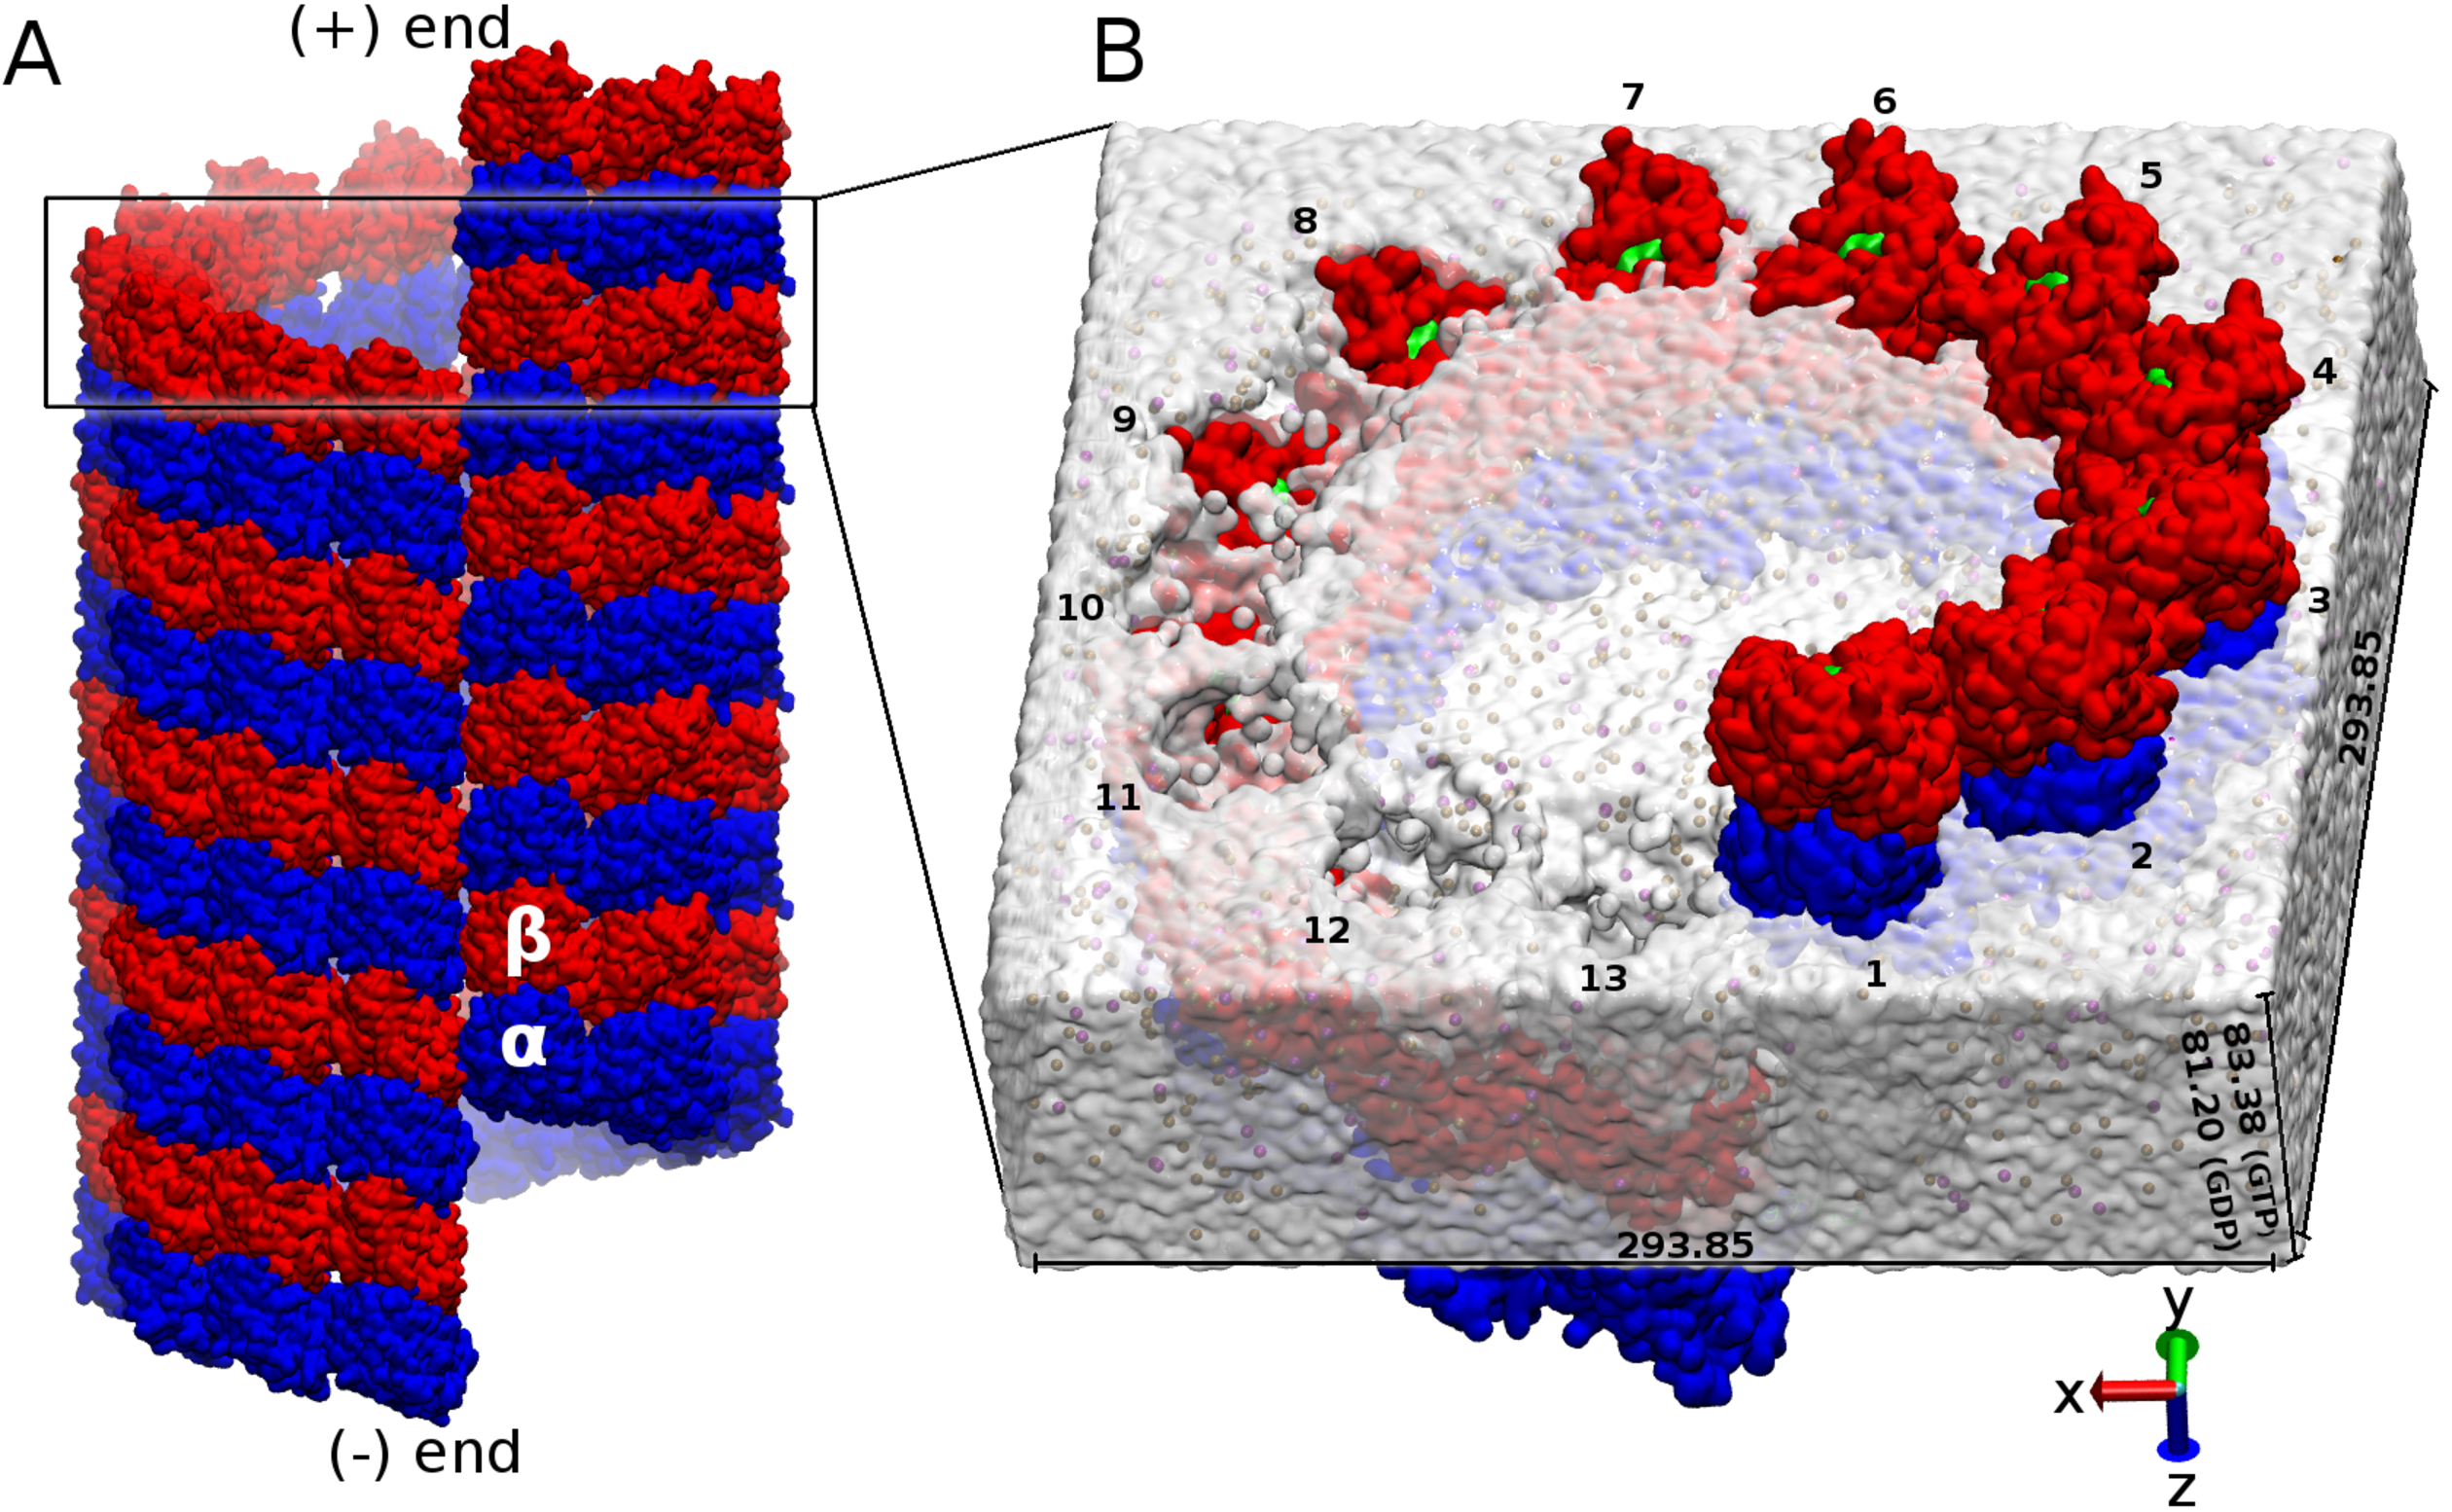
\includegraphics[width=0.98\linewidth]{images/Fig1.pdf}
  \caption[Model of MT structure]{Model of MT structure
  \\
      (A) A model of an MT lattice showing $\alpha$ (blue) and $\beta$ (red) tubulin subunits. It shows the plus and minus end as well as the seam.
      \\
      (B) A model of the system used in the molecular dynamics simulations.
      Tubulin dimers are numbered from 1 to 13,  GDP (or GTP) cofactor is shown
      in green within $\beta$-tubulin, the second GTP cofactor is buried between $\alpha$ and $\beta$ subunits, water is represented by the white box, within which
      purple spheres represent Cl\textsuperscript{-} and brown spheres represent Na\textsuperscript{+}.
      Periodic box dimensions in units of \AA\ are also shown.}
    \label{fig:System}
\end{figure*}

Several studies have been conducted to determine which specific structural
transitions that accompany GTP hydrolysis or taxol binding are
responsible for their effect on MT stability, especially the transition of the tubulin dimer between its straight and curved states \cite{Mandelkow1991,Hyman1995,Nogales2006,Barbier2010,Alushin2014}. In the
most recent of these studies, Alushin et al. found that GTP hydrolysis
leads to a compaction around the E-site nucleotide which is reversed
upon taxol binding \cite{Alushin2014}. This compaction was proposed to generate a strain 
which is powered by the energy of GTP hydrolysis and is believed to be released only through
outward curving of protofilaments, initiating disassembly \cite{Mitchison2014}. A missing component in these studies, however, 
is the quantification of the free energy changes that accompany these
structural transitions. Due to the difficulties related to its experimental measurement,
many simulations have been conducted to study detailed MT energetics
\cite{Erickson1981,VanBuren2002,Sept2003,Drabik2007,Andre2012,Kononova2014}. In a recent study 
we have analyzed the strength of hydrogen bonds that bring and hold tubulin
subunits together within different lattice configurations \cite{Ayoub2014}.
However, in all of these simulations, several factors were still missing. Most importantly, the full energetics of a complete MT model, 
which is essential to understanding the thermodynamics of tubulin assembly, has not been estimated yet due to the high computational price associated with such analyses. A detailed energy balance involving contributions due to each residue,
domain or subunit, to the best of our knowledge, was never
considered.

As a result of recent advances in computational technology, GPU-based computations can now be
implemented to perform very demanding calculations in a reasonable 
amount of time. With this technology readily available,
we simulated two complete all-atom MT models and studied in detail
their energetics. The models studied are: (a) an MT with GDP in the E-site (GDP-Model) and (b) an MT with GTP in the E-site (GTP-Model). We did not
need to look for a non-hydrolyzable analogue of GTP as hydrolysis is
not a problem in molecular dynamics simulations, in contrast to experimental
procedures \cite{Mitchison2014}.
The MT model that we used was initially built by Wells and 
Aksimentiev \cite{Wells2010} utilizing sophisticated theoretical techniques to combine experimental
structural information from a cryo-electron microscopy map of
MT at
8 \AA\ resolution \cite{Li2002} and electron crystallography structure of
tubulin at 3.5 \AA\ resolution \cite{Lowe2001}. We combined
this model with the recently published crystal
structures
\cite{Alushin2014} in order to generate an atomistic representation involving 
an infinite number of infinitely long MTs. This is possible due to the use of periodic boundary conditions.

\section{Methodology}
\label{Methods}

\subsection{Building the Models} 
\label{Methods_buildMod}
The recent structures for \gls{gmpcpp} and GDP bound MTs at resolutions of 4.7 and 4.9 \AA\ respectively
\cite{Alushin2014}, represented
an excellent starting point for building the models presented here. The 3$\times$3 lattice 
PDB structures of 3J6E (with GMPCPP) and 3J6F (with GDP) were
processed using MOE software \cite{moe} by the addition of hydrogens
and prediction of ionization states. The central tubulin dimer of the 
3$\times$3 lattice in each case was separated and was repaired by addition 
of the missing residues (Residue 1 in $\beta$-tubulin and residues 1,39 to 48, 440
in $\alpha$-tubulin) from the PDB structure 1TUB \cite{Nogales1998},
using MOE. We modified GMPCPP into GTP since in our simulations there is no
need to use the nonhydrolyzable GTP analogue as hydrolysis is not
expected in MD simulations. Next, for both GTP and GDP systems, the repaired
tubulin was superimposed over the 13 tubulin dimers in the complete
MT model built by Wells and Aksimentiev \cite{Wells2010}, producing 
a hybrid complete MT model for both systems. Thus,
we produced two models, the GTP-Model and the GDP-Model, by combining the 
helical
structural configuration developed by Wells and Aksimentiev
with the lattice tubulin coordinates obtained from Alushin's model.
Several clashes existed at lateral interfaces between tubulin dimers and were
resolved through a short minimization using the Generalized Born (GB) 
continuum model
in Amber \cite{case2012}.

Each model, as shown in Figure \ref{fig:System}B, has 13 tubulin dimers in an MT
orientation. For the GDP-Model, each tubulin has GTP, Mg\textsuperscript{2+} and
four coordinating water molecules at the $\alpha$-tubulin N-site, and GDP at the $\beta$-tubulin E-site.
For the GTP model, there was GTP, Mg\textsuperscript{2+} and
four coordinating water molecules at both the N-site and the E-site. 
Solvation was carried out using box of dimensions 293.85 $\times$ 293.85 $\times$ 83.38 (or 81.20) \AA$^{3}$ for the GTP- and GDP-Models, respectively. The $z$-component was obtained from Alushin's lattice structure 
\cite{Alushin2014} and ensures perfect longitudinal
alignment of tubulin dimers in both systems (see Figure \ref{fig:System}B). 
Both $x$ and $y$ components were obtained from Wells' structure \cite{Wells2010}. 
A total
of 181,000 TIP3P water molecules were added in the solvation box. This number
was obtained based on several optimization trials which 
guaranteed consistency in box dimensions and density throughout the simulations.
A total number of 442 Na$^{+}$ ions was needed for neutralizing the GTP-Model, versus 455 for the GDP-Model. An extra 
327 Na$^{+}$ and Cl$^{-}$ ions were added to bring the salt 
concentration to 0.1 M. 

During
the addition of water and ions, we made sure that no atoms were placed in positions which will be occupied by the periodic images
of our system in both the positive and negative $z$ direction (see the 
gaps in the water box of Figure \ref{fig:System}B) . Thus,
exploiting the periodic boundary conditions, the replication of our nearly 720,000-atom system in all directions should effectively result in
an infinite number of infinitely long MTs.
The AMBER Molecular Dynamics package was used for solvation, ionization,
and dynamics \cite{case2012}.

\subsection{Parameterization and Dynamics} \label{Methods_param}The all-atom forcefield
AMBERff12SB was used to parameterize the protein \cite{Cornell1995,Hornak2006}.
Cofactors were parameterized utilizing the parameter set
developed by Meagher et al. \cite{Meagher2003}. Each of the two systems was then 
minimized through nearly 1000 steps of the steepest
descent algorithm followed by about 6000 steps of the conjugate 
gradient algorithm. 
Then, the systems were heated, with restraints of \mbox{10 kcal mol$^{-1}$ \r{A}$^{-2}$} on the protein, to a temperature of
310 K using the Langevin thermostat over 20 ps under constant volume.
This was followed by 200 ps of density equilibration under constant temperature
and pressure, in which the restraints were eliminated gradually, followed by a production phase of 50 ns for each system.
Simulations were performed using NVIDIA Tesla K20X GPU cards on the PharmaMatrix
Cluster (University of Alberta) through AMBER GPU-accelerated code
\cite{Salomon-Ferrer2013,Gotz2012,LeGrand2013}.
All simulations were performed using periodic
boundary conditions employing the particle-mesh Ewald method for
treating long-range electrostatics with a non-bonded cut off of
10.0 \r{A} under constant pressure with anisotropic 
volume rescaling.

\subsection{Trajectory Analysis}
\label{Methods_analysis} 
The 50-ns trajectory of each system was analyzed for 
several structural and conformational aspects.
Most of the analysis was done utilizing the CPPTRAJ module in 
AMBER \cite{Roe2013}, MM/GBSA implementation in
AMBER \cite{Miller2012} plus several scripts that we designed
to facilitate data analysis. The software VMD 1.9.1
was also used for viewing trajectories and image rendering \cite{Humphrey1996}.

Data analysis included calculating the total as well as 
the per-residue MM/GBSA binding energies \cite{Kollman2000} between pairs of tubulin dimers in lateral and longitudinal orientations. These calculations
involved all the 13 heterodimers included in the simulations and would 
always give the energy per MT ring (Figure \ref{fig:System}B). Hence, energetic contributions
were assessed via the equation:
\begin{equation}
\label{eq:latE}
E_x = \epsilon_x(R_{13}L_{1}) + \sum\limits_{k=1}^{12} \epsilon_x(R_{k}L_{k+1})  
\end{equation}
for lateral systems, and the equation:
\begin{equation}
\label{eq:longE}
E_x = \sum\limits_{k=1}^{13} \epsilon_x(R_{k}L_{k}^{\prime})
\end{equation}
for longitudinal
systems. In both equations, $E_{x}$ represents an energetic contribution 
of a given residue, domain or subunit $x$ per MT ring of 13 tubulin dimers
shown in Figure \ref{fig:System}B. In Equation \ref{eq:latE}, $\epsilon_{x}(R_{k}L_{k+1})$ 
is the energetic contribution of the same entity $x$ in a subsystem composed
of only tubulin $k$, treated as a ``receptor'', and tubulin $k+1$, treated as a ``ligand''. $\epsilon_x(R_{13}L_{1})$ does the same but at the lateral seam, taking
into account the flip between $\alpha$- and $\beta$-subunits.
In Equation \ref{eq:longE},
$\epsilon_{x}(R_{k}L_{k}^{\prime})$ carries the same concept except that the
ligand in a longitudinal subsystem is simply the periodic image of the receptor,
hence the prime.
Therefore, we ended up investigating 12 lateral subsystems plus one lateral subsystem
at the seam and 13 longitudinal subsystems, for each model. An illustration 
of each subsystem is shown in Figure \ref{fig:TubInt}.
This means
that the dimer whose M-loop is involved in lateral interactions
was termed ``receptor'' in lateral subsystems, and the dimer whose
$\alpha$-tubulin was involved in longitudinal interactions
was termed as ``receptor'' in longitudinal subsystems. This 
distinction was necessary since we noticed that the 
energetic contributions can vary between tubulin dimers acting as receptors and those acting
as ligands.

\begin{figure}[htbp]
	\centering
	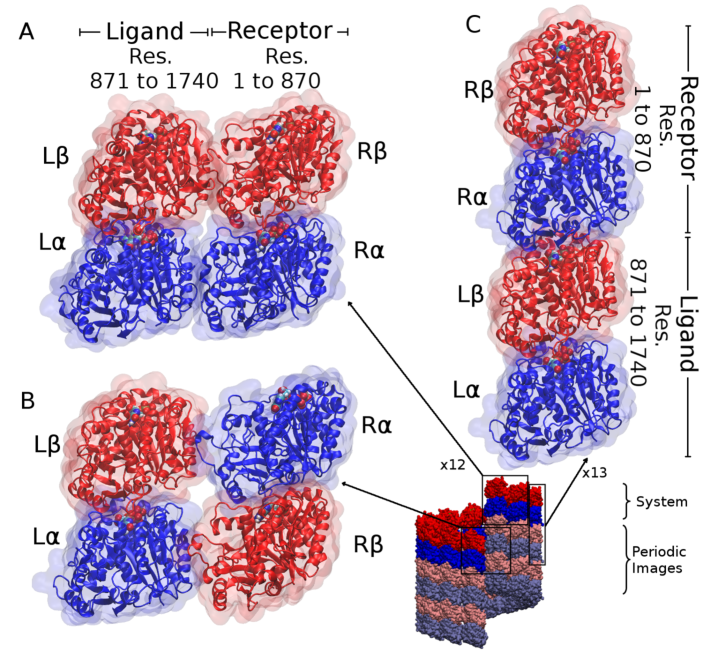
\includegraphics[width=0.8\linewidth]{images/Fig3.pdf}
	\caption[Tubulin subsystems used for MM/GBSA Calculations]{{Tubulin subsystems used for MM/GBSA calculations.}
		\\
		(A) A subsystem of two lateral tubulin dimers extracted
		from MT simulations where the receptor ($R$) is tubulin $k$
		and the ligand ($L$) is  tubulin $k+1$, where $k$ runs from 1 to 12,
		\\
		(B) Same as (A) but at the seam. I.e. the receptor is tubulin 13 and the ligand is tubulin 1. Residue (Res.) numbering in (A) and (B) are the same,
		\\
		(C) A subsystem of two longitudinal tubulin dimers where the receptor is
		tubulin $k$ and the ligand is its periodic image, where $k$ runs from 1 to 13.
		\\
		Total number of residues may differ slightly between the GDP and GTP models.}
	\label{fig:TubInt}
\end{figure}

All the energy calculations
were performed on 200 evenly-spaced snapshots from the last 10 ns of the molecular
dynamics trajectory where equilibration was confirmed.
A solvent and solute dielectric constant of 80 and 1, respectively, were used for electrostatics in the
Amber MM/GBSA implementation.

\section{Results and Discussion}

\subsection{Molecular Dynamics Equilibration}
A 50-ns MD trajectory was analyzed for several
equilibration aspects, the first of which is
the root-mean-square deviation (RMSD) of the backbone atoms relative to the starting
structure. In addition, two nearly perpendicular
MT cylinder diameters, namely \emph{Dx} and \emph{Dy}, were also calculated  along the trajectory. Referring 
to the tubulin dimer numbering in Figure \ref{fig:System}B, 
the diameter \emph{Dx} was defined as
the distance between the center of mass of dimer 4
and the center of mass of dimer 10 and 11, while \emph{Dy} 
was defined as the distance between the 
center of mass of dimer 1 and the center of mass of dimer 7 and 8. 
In both diameters, only the distance
projection on the \emph{x}-\emph{y} plane was considered
as this is what gives the cylinder diameter. 
Plots showing the change in RMSD of the backbone atoms,
\emph{Dx} and \emph{Dy} over simulation time for the
GDP- and GTP-Models are shown in Figures \ref{fig:Diam}A and \ref{fig:Diam}B.
The two diagrams indicate a strong correlation between fluctuations
in RMSD and in diameters which indicates that most of 
RMSD fluctuations are due to changes in the circular shape
of MT cylinders rather than the rearrangement of domains.
The two diagrams also show the flexibility of MT cylinders as they deform
spontaneously from a circular to an oval shape and vice versa. 
\begin{figure}[h]
  \centering 
  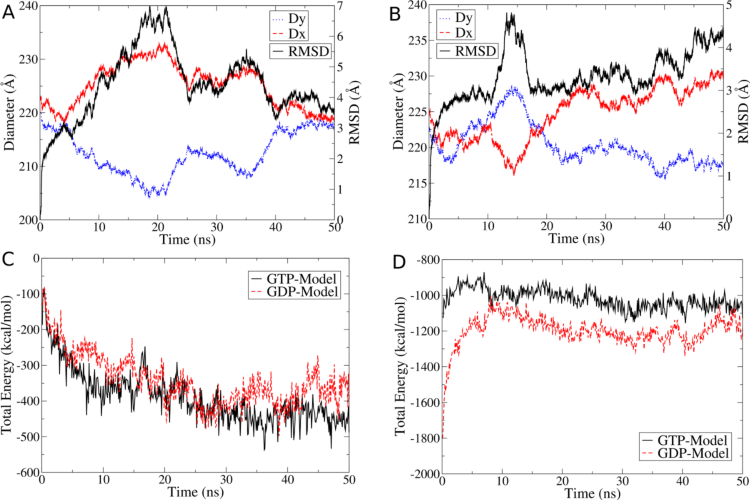
\includegraphics[width=0.9\linewidth]{images/Fig2.pdf}
  \caption[Equilibration Plots]{{Equilibration plots.}
    \\
    Plots showing the change in RMSD
    of protein backbone atoms and the two nearly
    perpendicular diameters \emph{Dx} and \emph{Dy} over simulation
    time in (A) GTP-Model and (B) GDP-Models.
    \\
    Equilibration of total sum of interaction energies versus simulation time across
    (C) lateral and (D) longitudinal inter-dimer interfaces.}
  \label{fig:Diam}
\end{figure}

Since our particular interest is in the MT energetics, we used the overall
MT energy across lateral and longitudinal inter-dimer interfaces as an 
indication of whether the system is equilibrated or not.
Hence, we calculated these energies using MM/GBSA and the
formulae in Equations \ref{eq:latE} and \ref{eq:longE} and plotted the
total energy per MT ring versus simulation time (Figures \ref{fig:Diam}C and \ref{fig:Diam}D).
Both plots indicate that the overall lateral and longitudinal 
energies in both the
GDP- and GTP-Models have already equilibrated at least before
the last 20 ns of the MD simulation time.
The plots also show that the large fluctuations in RMSD or $Dx$ and $Dy$
hardly affect the MT energetics at either of the two interfaces, which is
a good indication of the energetic
stability of our models.

\subsection{Lateral Energetics in the GDP-Model}

Total breakdown of the predicted energy contributions enabled us to perform
the analysis
for different residues, domains, subunits, and dimers
across both lateral and longitudinal inter-dimer interfaces.
Before listing the results, it should be noted that
energies calculated via the MM/GBSA method do not
necessarily reflect absolute energy values. Rather,
they are used for relative comparison within the same
model \cite{Hou2011}. It should also be noted
that all energies listed here are calculated per MT ring, unless
otherwise specified.

The overall energy of interaction across the 13 lateral
tubulin interfaces (see Figure \ref{fig:System}B), $E_{tot}^{lat}$, was found to be
$-411\pm29$ kcal/mol, nearly 60\% of which is due
to $\alpha$-$\alpha$ interactions and the rest
is due to $\beta$-$\beta$ interactions.
On the other hand, the contribution of the dimer
acting as a receptor (see Figures \ref{fig:TubInt}A and \ref{fig:TubInt}B), $E_{R}^{lat}$, was about 54\%
of the overall energy while the rest
was attributed to the ligand, $E_{L}^{lat}$, with
the difference entirely attributed to solvation
effects rather than direct interactions. It should be noted,
however, that the $\alpha$ subunit of the ligand (L$\alpha$)
and the $\beta$ subunit of the receptor (R$\beta$) together
contribute $-312\pm29$ kcal/mol which is nearly
75\% of $E_{tot}^{lat}$, with the L$\alpha$ contribution slightly 
larger than that due to R$\beta$. The contribution of L$\beta$ and R$\alpha$
was found to be much smaller, only 25\% of $E_{tot}^{lat}$. Upon structural inspection, this 50\% difference, being almost entirely due to electrostatic interactions, was attributed to diagonal interactions
between subunits; although the interface between 
L$\alpha$ and R$\beta$ is dominated by oppositely-charged residues and thus stabilizing the interaction, the opposite is true at the destabilizing
interface between R$\alpha$ and L$\beta$ which has, for 
example,
residues R$\alpha$/Glu220 and L$\beta$/Asp130 destabilizing the lateral interface by 
$12\pm1$ and $10\pm2$ kcal/mol, respectively.



As to the energetic breakdown according to interaction types, the contribution of the van 
der Waals and non-polar solvation energy, $E(\text{vdW}+\text{SA})$, to the overall energy is largely stabilizing with an average value of $-1476$ kcal/mol, 85\% of which is 
due to the \gls{vdW} interactions.
This stabilization is opposed by destabilization 
due to electrostatic interactions; the average sum of electrostatic and the polar solvation
energy, $E(\text{ele}+\text{GB})$, is $1065$ kcal/mol. This is expected
since tubulin dimers are highly
negatively charged and tend to
repel each other.

Regarding the detailed energy contributions per individual residues, the most important
residue across the lateral interface was found to be R$\beta$/Tyr283
followed by R$\alpha$/His283 and L$\alpha$/His88,
with overall stabilization energies of $-90\pm5$, 
$-47\pm5$ and $-42\pm3$ kcal/mol per MT ring, respectively. R$\beta$/Tyr283 alone
supplies more than 20\% of lateral stability
most of which is due to the vdW interactions. In fact,
most of the stabilizing residues on top of our list
were neutral ones with a strong stabilizing vdW 
component. On the other hand, almost all of the 
destabilizing residues were charged ones
with a strong electrostatic component,
most destabilizing of which is L$\beta$/Lys124 
with an energy of $22\pm7$ kcal/mol. A complete list 
of the different energetic contributions of each 
residue in the ligand and receptor per MT ring is
available in \cite{Ayoub2015}.

Domain contributions to the overall energy per MT ring were also 
calculated and Figures \ref{fig:DomainsLat}A and \ref{fig:DomainsLat}B
shows the most relevant of them. The contribution of the M-loop in both $\alpha$ and
$\beta$ subunits is by far the largest, with
values of $-112\pm10$ and $-159\pm10$ kcal/mol, respectively,
making up about two thirds of the energy of the overall lateral interactions.
This agrees well with previous predictions, although precise
values of their energetic contributions were never
calculated \cite{Nogales1999,Snyder2001,Li2002}.
Other less important domains are the L$\alpha$/N-terminal loop, L$\alpha$/H2-S3
loop, L$\alpha$/H3 helix and L$\alpha$/H9 helix at the $\alpha$ interface
with a stabilization of $-72\pm6$, $-62\pm6$, $-57\pm10$
and $-16\pm7$ kcal/mol, respectively \cite{Nogales1999,Li2002}.
L$\beta$/H3 helix at the  $\beta$-$\beta$ interface, however, has a strongly
destabilizing effect of $37\pm8$ kcal/mol. This 
supports previous predictions based on
structural analysis by Li et al. and Nogales et al;
however, these authors did not specify if these interactions are stabilizing or not \cite{Nogales1999,Li2002}. 
Additionally, L$\beta$/H2" helix and L$\beta$/H1'-S2 loop also have relatively 
strong stabilizing contributions of $-52.6\pm7$
and $-43\pm5$ kcal/mol, respectively. 

\begin{figure*}[h]
  \centering
  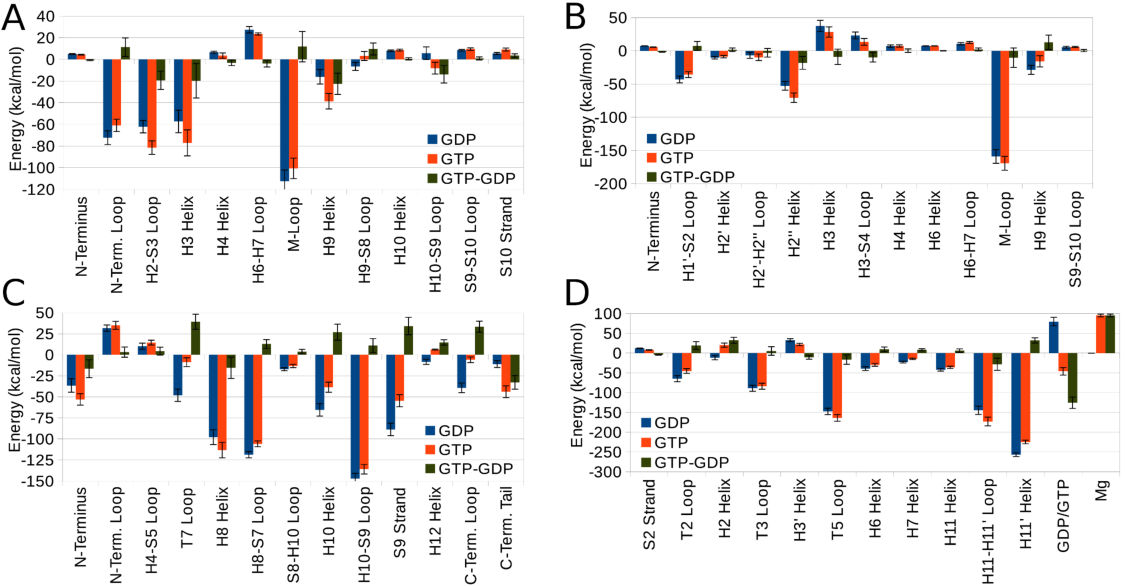
\includegraphics[width=0.99\linewidth]{images/Fig4.pdf}
  \caption[Domain contributions to overall energy]{{Domain contributions to overall energy.}
  \\
  Energetic contributions of important domains across lateral interface
  in (A) $\alpha$ and (B) $\beta$ subunits and 
  across longitudinal inter-dimer interface in (C) $\alpha$ and (D) $\beta$
  subunits. Data are shown
  for GDP- and GTP-Model as well as the difference between them (GTP-GDP). On the $x$-axis of (A) and (B), domains H4 helix and before occur at lateral interface of the
  ligand while domains after that 
  occur at receptor lateral interface. In (C), all
  domains belong to receptor while all the domains in
  (D) belong to ligand.
  See ligand and receptor definitions in Figure 
  \ref{fig:TubInt}.}
  \label{fig:DomainsLat}
\end{figure*}

\subsection{Lateral Energetics in the GTP-Model}
The overall interaction energy across
the lateral interface in the GTP-Model, $E_{tot}^{lat}$, was found to be $-482\pm29$ kcal/mol, nearly 60\% of which 
is due to the $\alpha$-$\alpha$ interactions.
This average overall energy is $71$ kcal/mol (nearly 20\%) more stable than 
the overall energy of the GDP-Model which explains the role of GTP
in stabilizing MTs as will
be shown later. Nearly 90\% of this difference in
stability is solely attributed to 
enhancement of the contribution of the ligand, 
both $\alpha$- and $\beta$-subunits, rather
than the receptor. 
As was noticed in the
GDP-Model, L$\alpha$ and R$\beta$ are also
responsible for most of the lateral 
stabilization in the GTP-Model, -$338\pm22$ kcal/mol (70\% of $E_{tot}^{lat}$).

Upon breakdown of the interaction energy to its individual components, we find that
in the GTP-Model, the $E(\text{vdW}+\text{SA})$ contribution becomes
$-1432$ kcal/mol while $E(\text{ele}+\text{GB})$ becomes
$950$ kcal/mol. Comparing this to the GDP-Model, it turns 
out that GTP destabilizes the vdW and non-polar solvation interactions by 
$44$ kcal/mol and stabilizes electrostatic and polar solvation 
interactions by $115$ kcal/mol, which results in the net stabilization of
$71$ kcal/mol as mentioned earlier. This difference becomes clear 
by analyzing Figures \ref{fig:DomainsLat}A and \ref{fig:DomainsLat}B for domain
contributions and Figure \ref{fig:Residues} for residual contributions.
It is apparent from Figure \ref{fig:DomainsLat}A that GTP strengthens
the contributions of the L$\alpha$/H3 helix and R$\alpha$/H9 helix by 
$23\pm10$ and $20\pm16$ kcal/mol, respectively.
Most of this helix stabilization can be attributed to interactions
involving R$\alpha$/Glu290 (residue number in Figure \ref{fig:Residues}, $i$, is 290), residue 
L$\alpha$/Asp127 ($i$=998), and residue
L$\alpha$/Arg123 ($i$=994). These three residues stabilize the
GTP-Model over the GDP-Model by energy values of 31, 20 and 19 kcal/mol, respectively, mostly due to electrostatic interactions.
Upon structural analysis it is apparent that GTP slightly 
rotates the dimer acting as a ligand toward the one
acting as a receptor, thus allowing
stronger interactions between H3 and H9 with oppositely-charged residues.
GTP also enhances
the stability imparted by the L$\alpha$/H2-S3 loop and the
R$\alpha$/H10-S9 loop, although it moderately decreases the role
of the
L$\alpha$/N-terminal loop as well as the R$\alpha$/M-loop in the overall MT stability.

\begin{figure}[h]
  \centering
 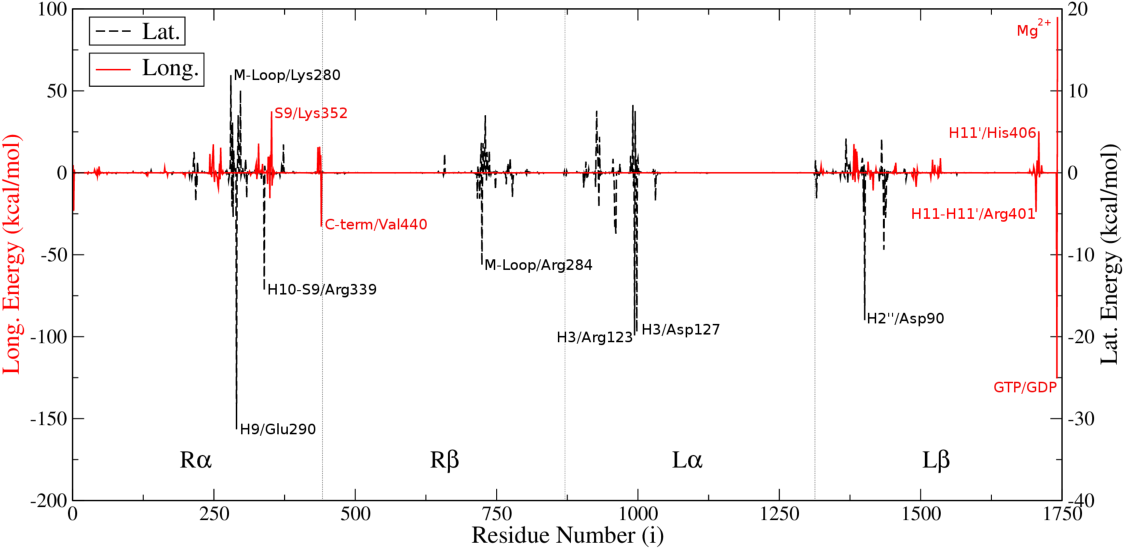
\includegraphics[width=0.99\linewidth]{images/Fig5.pdf}
 \caption[Energetic contributions of residues]{ {Energetic contributions of residues.} Difference between overall residual contributions per MT ring in GTP- and GDP-Model; ($E_{i}^{\text{GTP}} - E_{i}^{\text{GDP}}$), where $i$ is the residue number running from 1 to 1742. Different energy axes are used due to differences in magnitude of interactions at both interfaces. Important residues are labeled.}
  \label{fig:Residues}
\end{figure}

Similar conclusions are reached in regard to the 
$\beta$-subunit and the effect of the L$\beta$/H2'' helix
through residue L$\beta$/Asp90 ($i$=1401) and the R$\beta$/M-loop 
through residue R$\beta$/Arg284 ($i$=724).
Both domains are stabilized in the GTP-Model
by extra $18\pm10$ and $10\pm15$ kcal/mol compared to the GDP-Model, respectively.  
The charged nature of all these residues explains 
why most of GTP stabilization is manifested
in $E(\text{ele}+\text{GB})$ not $E(\text{vdW}+\text{SA})$.
Figure \ref{fig:DomainsLat}B also shows
that GTP reduces the destabilization caused by the L$\beta$/H3 helix
and the L$\beta$/H3-S4 loop. On the other hand, GTP reduces 
stability imparted by the
L$\beta$/H1'-S2 loop and the R$\beta$/H9 helix.
Details of the contribution of each residue in the 
GTP-Model is
available in \cite{Ayoub2015}.
.

\subsection{Longitudinal Energetics in the GDP-Model}

Analysis of the strength of interactions across the 
longitudinal inter-dimer interface in the GDP-Model yielded
an overall energy of $-1240\pm32$ kcal/mol
per MT ring, which is
nearly three times the lateral interaction 
energy. This is in agreement with structural
observations \cite{Nogales1999}. Due to the orientation of tubulin dimers 
at the longitudinal inter-dimer interface, the contributions 
of L$\alpha$ and R$\beta$ are essentially zero and 
will always be neglected here. On the other hand,
the contribution of L$\beta$ is 54\% of the total value,
and the remainder is contributed by R$\alpha$.
The breakdown of this energy yields an average $E(\text{vdW}+\text{SA})$
of $-2668$ kcal/mol which is almost twice 
as large as the value across the lateral interface. This
is obviously due to the tighter packing of the 
residues here as opposed to looser packing at the
lateral interface.
The average $E(\text{ele}+\text{GB})$ across the longitudinal inter-dimer
interface is $1428$ kcal/mol and it is 34\% larger
than its value at the lateral interface.

Per-residue energy analysis reveals the most important residues
to longitudinal stability, the first of which
is L$\beta$/Arg401 from the H11-H11' loop
which alone supplies $-101\pm7$ kcal/mol (nearly
10\%) \cite{Ayoub2014}. After that come residues L$\beta$/Phe404
and L$\beta$/Trp407 from the H11' helix
both of which support
longitudinal stability by contributing $-91\pm3$ and
$-78\pm3$ kcal/mol, respectively. This makes the two
former domains,
which constitute part of the tubulin C-terminal domain, the most critical for 
longitudinal stability in the $\beta$-subunit
(Figure \ref{fig:DomainsLat}D). The figure also shows that 
the following domains: the T5 loop, T3
loop, and T2 loop are also very important for longitudinal
stability. The role of the GDP cofactor appears quite
influential at the longitudinal inter-dimer interface, in contrast to the
lateral one. It is primarily destabilizing 
with a large contribution of $79\pm11$ kcal/mol
due mainly to a strong electrostatic repulsion with the 
highly negative environment, despite its strong salt bridge
with R$\alpha$/Lys352. Residual analysis of the R$\alpha$
subunit also shows some relatively less important
residues; R$\alpha$/Trp346, R$\alpha$/Tyr262 and R$\alpha$/Lys352
with energy contributions of nearly $-60$ kcal/mol for each of them.
These and other
residues are responsible for the following domains: the 
H10-S9 loop,
H8-S7 loop, and the
S9 strand being the top stabilizers in Figure \ref{fig:DomainsLat}C.
The H8 and H10 helices are also relatively 
important for longitudinal stability. Both the
C- and N-terminal domains are important as well,
with the N-terminal loop being a destabilizer,
in contrast to its role at the lateral interface.

\subsection{Longitudinal Energetics in the GTP-Model}
The overall interaction energy across the longitudinal inter-dimer
interface in the GTP-Model was found to be $-1098\pm30$
kcal/mol per MT ring, which is 141 kcal/mol (10\%)
less stable than the
GDP-Model system. This difference is attributed to 
a 7\% decrease in the R$\alpha$ and 3\% decrease in the L$\beta$ interactions.
Upon energetic breakdown we see that GTP destabilizes the
vdW and non-polar solvation energy by nearly 250 kcal/mol,
while stabilizing electrostatic and polar solvation energy by
nearly 110 kcal/mol. This could
be due to the longstanding
observation that GTP
leads to an expansion in the E-site
and lengthening of the tubulin dimers. That is, axial dimer repeat changes
from 81.20 \AA\ in the GDP-Model to
83.38 \AA\ in the GTP-Model
\cite{Hyman1995,Alushin2014}.
This reduces the packing of atoms 
at the interface and hence lowers
both the vdW attraction and electrostatic repulsion, the
former being affected most due
to its stronger dependence on 
distance.

Looking into domain contributions in Figures \ref{fig:DomainsLat}C and
D we see how GTP destabilization of longitudinal interactions
can be subdivided. The most pronounced difference between the GDP- and the
GTP-Model appears in regard to the cofactors at the E-site. Although GDP was largely destabilizing 
in the GDP-Model, GTP becomes relatively largely stabilizing,
with an energy change from the GDP-Model of nearly $125\pm14$ kcal/mol.
However, this change should not be considered without taking into account the
effect of the Mg\textsuperscript{2+} ion that accompanies GTP.
This magnesium ion introduces an instability of $95\pm4$ kcal/mol to the GTP-Model.
Hence, the overall effect of replacing GDP by GTP and a magnesium ion is
a stabilization of 30 kcal/mol
on average.
Other causes of the lack of stability in the GTP-Model L$\beta$
include the decrease in the contribution of the
H11' helix because GTP offsets interactions by
L$\beta$/His406 ($i$=1709) by as much as 25 kcal/mol. This is because
this histidine is protonated in the GTP-Model and neutral in
the GDP-Model and therefore behaves differently in both cases. Being charged in the
GTP-Model, it is distracted from the strong attractive vdW interactions it makes
with the R$\alpha$/H8-S7 loop by electrostatic and hydrogen bonds with other
residues in the L$\beta$ subunit.
GTP also causes longitudinal stabilization due to the domains: the H2 helix and the T2 loop 
whose contributions decline while causing stabilization due to the
H11-H11' loop and the T5 loop whose contributions rise. 
As to the R$\alpha$-subunit (Figure \ref{fig:DomainsLat}C),
stabilization due to several domains declines in the GTP-Model.
These domains include the T7 loop, the S9 strand, the C-terminal loop,
the H10 helix, the H12 helix, the H8-S7 loop, and the H10-S9 loop. In short,
the GTP-Model is longitudinally less stable than the GDP-Model in most of the 
domains occurring at the longitudinal inter-dimer interface. An exception to this rule
is the increased stabilization due to the C-terminal tail, the N-terminus
and the H8 helix, Figure \ref{fig:DomainsLat}C shows the extent of
stabilization or destabilization imparted by GTP on each domain.
We should also mention that the strong attraction of the R$\alpha$/T7
loop emerging after GTP hydrolysis (Figure \ref{fig:DomainsLat}C) could explain the proposed compaction
of the E-site after GTP hydrolysis \cite{Alushin2014}. In fact,
the overall increase in longitudinal dimer-dimer
attraction after GTP
hydrolysis, as shown by the different values of 
 $E_{tot}^{long}$ in both models, explains the driving 
force for this E-site compaction.

Among other important residues, R$\alpha$/Lys352 ($i$=352)
of the domain S9 strand has a largely reduced contribution in the
GTP-Model, as shown in Figure \ref{fig:Residues}, which is 37 kcal/mol
less stabilizing than in the GDP-Model. While having 
comparable vdW contributions in the two models, this residue
suffers strong repulsion probably
due to a nearby Mg\textsuperscript{2+} ion in the GTP-Model.
Another important residue is R$\alpha$/Val440, located in the C-terminus
of the $\alpha$-subunit in our model. GTP enhances the stabilization caused by
this residue by nearly
33 kcal/mol over the GDP-Model. Additional important 
residues and their contributions 
are
available in \cite{Ayoub2015}.

\subsection{Energy Profile Explains the MT Disassembly Mechanism}
Depolymerizing MTs display protofilaments that
peel into ``ram's horns'' formations under high magnesium
buffer conditions. The ends of MTs become frayed, however,
under physiological concentrations of magnesium \cite{Mandelkow1991}.
The energy profile throughout the longitudinal inter-dimer interface provides
a clear explanation for the disassembly mechanism, its driving force,
and its relation to Mg\textsuperscript{2+} concentration.
We characterized each residue in the longitudinal 
subsystems by its radial distance from the MT lumen in \AA, which 
was plotted on the $x$-axis. The interaction 
energies of residues, per MT ring, over half-closed intervals of $\left[x,x+3 \right)$ were summed up and
plotted on the $y$-axis to produce the radial energy profiles 
in Figures \ref{fig:Edist}A,
\ref{fig:Edist}B and \ref{fig:Edist}C. 

\begin{figure*}
  \centering 
  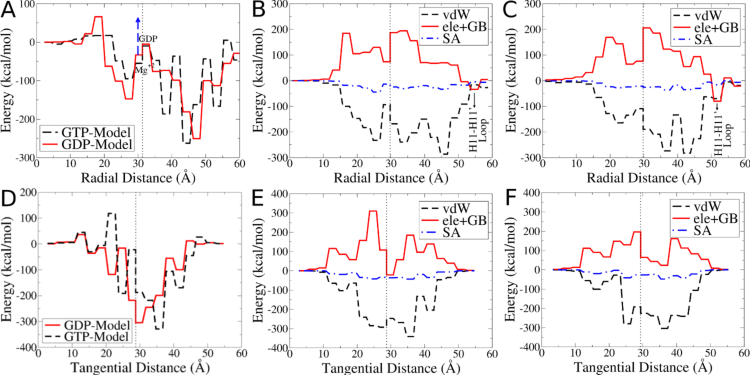
\includegraphics[width=0.99\linewidth]{images/Edist.pdf}
  \caption[Energy profiles at longitudinal inter-dimer interface.]{{Energy profiles at longitudinal inter-dimer interface.} 
  \\
  The figures
  shows the sum of energetic contributions of residues located at distance
  intervals of 3 \AA\ apart, plotted against the radial distance between 
  these residues and the MT lumen (A,B,C) or the tangential distance between the
  residues and laterally adjacent dimer (D,E,F) in GTP- and GDP-Model. Dotted lines represent the center of mass of tubulin.\\
  (A) Radial distribution of total energy in both models. Blue dashed arrow shows how destabilizing the effect of Mg\textsuperscript{2+} is on the GDP-Model if it remains
  after GTP hydrolysis.
  (B) Radial distribution of the energy components $E(\text{vdW})$, $E(\text{ele+GB})$ and 
  $E(\text{SA})$ in the GDP-Model and in (C) the GTP-Model,
  (D) Tangential distribution of total energy in both models. On the $x$-axis, $x<30$ is the intermediate domain and $x>30$ is the nucleotide binding domain. 
  (E) Tangential distribution of the energy components $E(\text{vdW})$, $E(\text{ele+GB})$ and 
    $E(\text{SA})$ in the GDP-Model and in (F) the GTP-Model.
  }
  \label{fig:Edist}
\end{figure*}

The diagram
in Figure \ref{fig:Edist}A leads to a striking observation that
the energy distribution throughout the longitudinal
inter-dimer interface is not even,
with the outward portion ($x > 30$ \AA) largely outweighing the inward portion ($x < 30$ \AA), with the center of mass
of tubulin being at $x \approx$ 30 \AA. To mention specific values, in the GTP-Model, the outward
portion provides nearly $-956$ kcal/mol while in the GDP-Model it provides
$-982$ kcal/mol, both values being larger than 80\% of the overall
longitudinal interaction energy. This uneven distribution of energy, 
or forces of attraction, is
proposed to yield a strong torque that
tends to curl MT protofilaments outwardly,
breaking lateral bonds and promoting disassembly as illustrated in 
Figure \ref{fig:Mech}A. 

Radial energy profiles
of different components of the interaction
energy are also shown in Figures 
\ref{fig:Edist}B and \ref{fig:Edist}C, where electrostatic
interactions cause very strong repulsion 
through the inward portion and attraction
only at the periphery where the H11-H11' loop and 
particularly residue L$\beta$/Arg401
are located. We propose
a pivotal role for this residue, and for
the entire C-terminal domain, in regulating
dynamic instability. Electrostatic repulsion 
by the inner domains
and attraction by the outer C-terminal
domain is the recipe 
for outward curling and
disassembly in MTs. The vdW distribution will also work, as shown in Figure \ref{fig:Edist}B for the GDP-Model and \ref{fig:Edist}C for the GTP-Model, to curl protofilaments
outward until the vdW contacts, and other components, are balanced out.

The largely destabilizing Mg\textsuperscript{2+} ion
(see Figure \ref{fig:DomainsLat}D) also plays an
important role. Even though
GDP at the E-site has low affinity for
Mg\textsuperscript{2+} \cite{Correia1987}, it
may still bind to Mg\textsuperscript{2+} if it is 
present in high concentrations
or Mg\textsuperscript{2+} may stay in the E-site after GTP hydrolysis. This largely destabilizes
the inner portion of the protofilament (blue
dashed arrow in Figure \ref{fig:Edist}A), allowing outward forces
to pull tubulin out with even less
resistance from the other side,
thus 
promoting outward curling and MT disassembly. This explains 
why large Mg\textsuperscript{2+} concentrations promote ram's horns 
formations \cite{Frigon1975} and increase the rate of disassembly \cite{Gal1988,Brien1990}, while its
low concentrations produce frayed ends and 
lower rates of disassembly \cite{Mandelkow1991}.

To explain MT disassembly from a free energy perspective,
Figure \ref{fig:Mech}A shows an illustration of the analyzed situation.
As already established, uneven distribution of attractive
interactions along the longitudinal inter-dimer interface favors outward curling. In the GTP-Model, outward curling is favored
by $-956$ kcal/mol of interaction energy outwardly with respect to the
center of mass of tubulin,
as compared to $-982$ kcal/mol in the GDP-Model.
These curl-favoring energies/forces are opposed by 
the lateral interaction energies which tend to pull
protofilaments back from both sides, i.e. double 
the effect. The magnitude of this 
effect is $2 \times E_{tot}^{lat}$, giving $-964$ kcal/mol in
the GTP-Model which is much larger than  $-822$ kcal/mol in the GDP-Model,
all energies given per MT ring.
We propose that this lateral inward pull
balances out the longitudinal
outward push in case of the GTP-Model.
That being said, the presence of a GTP
cap at the tip of the MT would prevent
outward curling and thus provide
stability for the entire MT structure.
After GTP hydrolysis reaches the cap, however,
lateral bonds become weaker
and longitudinal outward push manages
to break the lateral contacts, causing
outward curling and MT disassembly.
High concentrations of Mg\textsuperscript{2+} may also increase outward curling and the disassembly rate, as explained
earlier.

\begin{figure*}[h]
  \centering
 \includegraphics[height=3.8in]{images/Fig7.pdf}
  \caption[Mechanism of MT disassembly]{{\bf Mechanism of MT disassembly.}\\
  (A) Radial energy distribution of the GDP-Model at the longitudinal inter-dimer interface is superposed on a protofilament to show how uneven the
  energy distribution is. This produces a torque that leads to outward curling of the protofilament.
  (B) Tangential energy distribution of the GDP-Model showing slight sideway tilting
  due to the slightly uneven distribution of energy.
 $\alpha$-subunits are colored
  blue while $\beta$-subunits are red.}
  \label{fig:Mech}
\end{figure*}

Similar observations could be made about the tangential energy profiles at the longitudinal inter-dimer interface.
Figures \ref{fig:Edist}D, \ref{fig:Edist}E and \ref{fig:Edist}F show the tangential
energy profiles with the $x$-axis showing the 
distance from the laterally adjacent protofilament. On the $x$-axis, $x<30$ 
is the tubulin intermediate domain
while $x>30$ is the nucleotide binding
domain with $x\approx30$ being at the center of mass (see Figure \ref{fig:Mech}B). Figure \ref{fig:Edist}D shows that
in The GTP-Model, the distribution is
also uneven with right-side portion being $-1023$\,kcal/mol (nearly 93\% of the total) as compared to $-887$\,kcal/mol
(71\% of the total) in the GDP-Model. This means that in the GTP-Model, there is a strong force tilting it sideways. However, after
GTP hydrolysis and rearrangement of domains at
the longitudinal inter-dimer interface, that force largely decreases and the uneven distribution starts to balance out,
as shown in Figure \ref{fig:Edist}D,
decreasing the strain on lattice integrity. 
This is in perfect agreement with the recent findings of
Alushin et al. \cite{Alushin2014} They observed that
GTP hydrolysis and the release of an inorganic
phosphate group
leaves a hole within the longitudinal inter-dimer interface between tubulin dimers producing a strain which results in sideway tilting in the same direction
\cite{Mitchison2014}. In the present work we
show that this tilting is also driven by the uneven energy distribution along
the same direction as in the work of 
Alushin et al. \cite{Alushin2014} (see Figure \ref{fig:Mech}B). However, this sideway tilting should not be considered as the the driving force of disassembly since it is orthogonal to the outward curling. Combining the two effects together, we conclude that uneven distribution at the longitudinal inter-dimer interface generally leads to a large outward and slight sideway tilting of 
protofilaments, the former of which is
responsible for disassembly of GDP-bound MTs.  

\subsection{Energy Distribution around the Microtubule Ring}

As mentioned in the Methods section,
the MT ring was divided into 13 subsystems
of laterally adjacent tubulin dimers and another 13 subsystems
of longitudinally adjacent tubulin dimers
(see Figure \ref{fig:TubInt}). All of the 
energies presented earlier were expressed per MT ring, meaning that they were summed over the 13 subsystems. In this section,
however, we focus on the interaction energy in each 
subsystem. Figures \ref{fig:Ediag}A and \ref{fig:Ediag}B shows energy diagrams 
for lateral and longitudinal interactions superposed
over the MT ring. We first note that 
the shape of the lateral interactions 
(Figure \ref{fig:Ediag}A) in the GDP-Model
is very distorted with several ``kinks'' of very low 
energy. When compared to the GTP-Model, its shape is much
less distorted. This could come as a straightforward consequence of
the fact that GTP-Model is laterally more stable 
than the GDP-Model and hence suffers less ``deformations''.

\begin{figure}[h]
  \centering
  \includegraphics[width=0.9\linewidth]{images/MTdist.pdf}
  \caption[Energy diagrams of the complete MT ring]{{ Energy diagrams of the complete MT ring.}\\
  The diagram shows the magnitude of interaction energies
  at each interface between two tubulin dimers, whether
  at (A) the lateral interface, or at (B) the longitudinal inter-dimer
  interface. The magnitude of the interactions is proportional to the swelling at each interface with swellings
  in (A) being exaggerated to aid viewing.
  Green represents GTP-Model while red represents GDP-Model.}
  \label{fig:Ediag}
\end{figure}

It is worth mentioning that the deepest of the kinks in
the GDP-Model energy diagram, i.e. the interface
with the weakest interactions, is the one occurring at the seam
(between dimer 13 and dimer 1), in contrast to its 
strength in the GTP-Model. It has an energy of 
$-9\pm7$ kcal/mol which is very low compared to the one at the interface between dimer 12 and 13, for example,
which has an energy of interaction equal to
$-57\pm9$ kcal/mol. 
We predict that protofilaments number 1 and 13 having
very strong longitudinal contacts 
antagonized by
very weak lateral contacts at the seam,
will be the first to dissociate laterally
and curve outwards. This should open the MT 
cylinder which should then
trigger disassembly.
Therefore, MT energetics suggest that the seam
is the most labile part of the MT and could act as a trigger
point for disassembly. This is precisely what
was reported recently \cite{Katsuki2014}.


The energy diagrams at the longitudinal inter-dimer interfaces
(Figure \ref{fig:Ediag}B) appear to be more even
than at the lateral interfaces.
However, we see no major difference in the pattern between 
the GTP-Model and the GDP-Model except that longitudinal interactions in the GDP-Model
are stronger, which was established 
earlier.

\section{Conclusions}

We used sophisticated all-atom molecular dynamics simulations to produce accurate MT models, combined
with high resolution cryo-electron
microscopy maps, to generate an infinite
number of infinitely long MT representations. The MM/GBSA energy analysis that
followed the simulations enabled an
estimate of the contributions of 
individual residues, domains, subunits and dimers
toward the lateral and longitudinal stability 
of a complete MT ring.
We found that longitudinal interactions
are about two to three times stronger 
than lateral interactions explaining the greater stability of the MT structure along its axis than radially. This finding agrees with previous structural observations \cite{Nogales1999}
and computational estimations \cite{VanBuren2002,Kononova2014}.
We also found that 
interactions are not evenly
distributed radially along the longitudinal inter-dimer
interface. That is, attractive interactions
are largely concentrated away from the
MT lumen, producing a force that
curls protofilaments outward and eventually causing MT
disassembly.
The GTP-Model was laterally more stable than
the GDP-Model and the opposite was true for the longitudinal inter-dimer interface. 
Since lateral forces oppose outward
curling while longitudinal forces
support it, we expect the GTP-Model to 
be less prone to disassembly than the GDP-Model. With its lateral forces being
strong enough to prevent outward
curling caused by longitudinal forces,
the GTP-cap at the plus end can stabilize an entire 
MT cylinder.
After GTP hydrolysis reaches the cap,
lateral forces are too weak to 
prevent outward curling, especially at
the seam which has the weakest lateral
contacts. This results in outward curling
and microtubule disassembly.

We also confirmed that the MT seam 
is most likely to act as a trigger point for MT
disassembly by being the most labile
interface in the MT cylinder
\cite{Katsuki2014}.
Magnesium ion was demonstrated to be an influential
factor in MT stability. Being present at the
inner portion of the longitudinal inter-dimer interface, the largely destabilizing 
Mg\textsuperscript{2+} ion repels the inward 
portion and enhances outward curling,
the formation of ram's horns structures
and rapid disassembly, which is consistent with
key experimental findings \cite{Mandelkow1991}. This action
of Mg\textsuperscript{2+} at the E-site of tubulin
is suppressed by GTP in GTP-capped
MTs. As we showed earlier, the ensemble of
Mg\textsuperscript{2+} and GTP at the E-site
is collectively stabilizing. However,
hydrolysis of GTP and release of 
inorganic phosphate 
create a gap at the longitudinal inter-dimer
interface and leave the
largely destabilizing ensemble of
GDP and Mg\textsuperscript{2+} which
rapidly promotes outward curling
to fill this gap.
This happens only at large Mg\textsuperscript{2+}
concentrations since GDP at the
E-site has low affinity for Mg\textsuperscript{2+}
\cite{Correia1987}.
At low Mg\textsuperscript{2+} concentrations,
disassembly becomes slower and 
outward curling becomes less pronounced
\cite{Mandelkow1991}.

Tangential energy profiles at the
longitudinal inter-dimer interface were also shown to be uneven and
confirmed the hypothesis that GTP
hydrolysis produces a strain which promotes sideway titling 
\cite{Alushin2014,Mitchison2014}.
However, much of this strain could 
be tolerated within the lattice constraints and its orthogonality
to the direction of outward
curling rules out its role in
disassembly.

We also identified the most important residues and domains with respect to MT stability at both 
interfaces and their energetic contributions. At the lateral
interface, the $\alpha$/M-loop, $\beta$/M-loop, $\alpha$/H3 helix, $\alpha$/N-terminal loop and the
$\alpha$/H2-S3 loop were shown 
to be most stabilizing while the
$\beta$/H3 helix was actually 
destabilizing. This
supports predictions based on structural 
studies \cite{Nogales1999,Li2002}.
Residue $\alpha$/Tyr283
was shown to form a very strong
network of vdW interactions with neighboring residues and to
provide the largest amount
of stability at the lateral interface.
At the longitudinal inter-dimer interface,
the $\beta$/C-terminal domain was found to be 
of paramount importance not only 
to stability but also to the
mechanism of MT disassembly.
In particular, residues 
$\beta$/Arg401, $\beta$/Phe404, and
$\beta$/Trp407 of the C-terminal
H11 helix and the
H11-H11' loop were shown to provide
more than 20\% of longitudinal
stability in both the GTP- and GDP-Models.
The complete breakdown
of MT energetics per every single
residue was further analyzed in order to
provide crucial insights into many aspects
of MT dynamic instability.
Of highest importance is the 
calculation of the amount
of force generated through outward
curling due to uneven longitudinal
interactions. This could
help unravel many aspect of the
molecular machinery of cell
division, in particular the force generation requirement for chromosome segregation.

\chapter{Conclusion and Future Work}

In this thesis, I reported the study of MT structure and stability as
well as the effect of drugs on it. I carried out a virtual screening study based
on similarity of molecular fingerprints to six available MSAs, namely 
paclitaxel, epothilone A, eleutherobin, discodermolide, sarcodictyin A, and
laulimalide. The library was then docked to the taxol binding site and the hits
were analyzed for novelty. The most novel hit was optimized visually to 
increase its binding affinity as well as its pharmacokinetic profile.
Rescoring of the binding energies confirmed my predictions about the affinities
of the proposed molecules. The proposed molecules were predicted to have much higher affinities to the taxol binding site than the available MSAs, with
reasonable pharmacokinetic profiles.

Due to the difficulty in synthesizing these novel hits, I looked for the available 
molecules which have structures that resemble my novel hits, which turned out
to be the antibiotic family of lankacidin. Based on similarity to my novel hits,
lankacidin C was hypothesized to bind to the taxol binding site. Docking
and MM/PBSA rescoring of the binding of lankacidin C to the taxol binding site
confirmed this hypothesis computationally. Together with my collaborators, we made
an experimental design to prove this hypothesis using laboratory experiments. 
Fluorescence quenching experiments showed that both lankacidin C and lankacidinol 
A affect the conformation of tubulin, specifically that of TUB-B1,
in a concentration-dependent manner, thus confirming the binding of lankacidin
antibiotics to the $\beta$-tubulin subunit of the tubulin dimer.
This sheds the light on the unknown antitumor mechanism of action of lankacidin
antibiotics and strengthens the possibility that its antitumor action is separate
from its antimicrobial action, the latter being associated with
interference with protein synthesis. As a future plan, the binding of lankacidin
to the taxol binding site will be tested through the displacement of
fluorescent taxoid, Flutax-2, which will prove whether lankacidin binds to the
taxol binding site of $\beta$-tubulin or not. Also, tubulin polymerization
assays are now being performed to study the effect of lankacidin on the
stability and polymerization rate of microtubules. If our hypothesis is
established, lankacidin structure may be further optimized for perfect fit in the binding
pocket to improve its affinity as well as pharmacokinetic parameters.

In another direction, I also investigated the stability of MT structure and
the thermodynamic aspects of the binding between tubulin dimers
within an MT lattice. I first started by investigating the hydrogen bonds
between tubulin dimers. This required the development of a robust and affordable
methodology for estimating the hydrogen bond energies. For that purpose, I 
investigated the utility of quantities like Mulliken overlap population,
Wiberg bond index, overlap-weighted bond orbital, and electron density at bond critical point in estimating hydrogen bond energies following a DFT 
calculation and population analysis. The effect of diffuse functions in 
the basis sets used as well as the effect of dispersion were also assessed.
I determined that the most robust and
affordable method for estimating hydrogen bond energies was the 
use of the descriptor $\rho$ which is the electron density at the 
bond critical point following a QTAIM analysis. The functional B3LYP as
well as the basis set TZVP were chosen as the most suitable
level of theory. Linear fitting parameters for each of the four studied descriptors were provided and they could be used directly to estimate hydrogen
bond strengths.

The strength of the hydrogen bonds bringing tubulin dimers together laterally and
longitudinally was assessed utilizing the aforementioned parameters and descriptors.
The overall as well as the pairwise hydrogen bond energies were calculated.
The study revealed the importance of hydrogen bonds in general in tubulin
energetics. The study showed that hydrogen bonds at the lateral interface 
are stronger than that at the longitudinal interface although when the overall MM/GBSA
energy is considered, the opposite is true. The $\beta$-$\beta$ interactions
were comparable to the $\alpha$-$\alpha$ interactions in the B-lattice in a 95\% confidence
interval.
The study also showed that the stability of the B-lattice configuration is comparable to that of
the A-lattice when hydrogen bonds are concerned. This suggests that other energetic contributions
could be responsible for the observed difference in predominance between the two lattice forms.
Pairwise hydrogen bond energies were in good agreement with experimental data and
could be used in many several analysis regarding the energetics of tubulin
dimer-dimer interactions.

Finally, a molecular dynamics simulation of a complete MT model was carried
out utilizing periodic boundary conditions to simulate an infinite number 
of infinitely long MT cylinders. The trajectory provided through these simulations
were analyzed to calculate the overall as well as per-residue MM/GBSA
binding energies between residues at lateral or longitudinal interfaces
all along the MT cylinder.
The energetic analysis revealed the stability contribution of each residue, domain,
subunit, and dimer to the overall stability of an MT cylinder. 
Since two systems were modeled, GDP- and GTP-Model, the comparison of the
two gave insight regarding the role of GTP-hydrolysis in MT stability and
disassembly. The study also allowed to propose a detailed explanation
of the driving force behind MT disassembly, which is the uneven distribution
of binding energy along the longitudinal interface. With the outer portion
largely outweighing the inner one, a torque is generated curling protofilaments
outward and only opposed by the lateral bonds between protofilaments. Since 
lateral bonds are
stronger in the GTP-Model than in the GDP-Model, outward curling and hence
disassembly happens often after GTP hydrolysis and not before, confirming the
GTP-cap model.

It would be prudent, however, to carry out a simulation of a free protofilament
in order to find out about the
effect of uneven longitudinal 
energy distribution on the
extent of outward curling. By comparing
the energy of a free protofilament
to the energy of a protofilament constrained 
within our MT model, we can 
predict the amount of free
energy released by outward curling
and additional light could be shed on the
mechanism and driving forces in MT
disassembly and force generation due to microtubule shortening. In this
way, chromosome segregation could be better understood.
Also, simulating a GDP-Taxol case
would be necessary to understand the molecular mechanisms
by which taxol bound to an MT prevents outward
curling and MT disassembly. This constitutes a plan for our future work
in this project.


%TCIMACRO{
%\TeXButton{liography in contents}{\clearpage\addcontentsline{toc}{chapter}{Bibliography}
%\singlespacing
%}}%
%BeginExpansion
\clearpage\addcontentsline{toc}{chapter}{Bibliography}
\singlespacing
%
%EndExpansion
%
%
%
%
%
%
%
%
%
%
%
%
%
%
%
%
%
%
%
%
%
%
%
%
%
%
%
%
%
%
%
%
%
%
%
%
%
%
%dont forget this if you want the bibliography to show up on the contents page
\bibliographystyle{initunsrt}
\bibliography{thesis}
\bigskip 
%Generates the bibliography. You have to specify the source bib files and the biblio style 

%TCIMACRO{
%\TeXButton{Appendices}{\appendix
%}}%
%BeginExpansion
\appendix
\includepdf[pages=1-10]{supp.pdf}
%
%EndExpansion
%
%
%
%
%
%
%
%
%
%
%
%
%
%
%
%
%
%
%
%
%
%
%
%
%
%
%
%
%
%
%
%
%
%
%
%
%
%
%The chapters after this tab are all appendices

\end{document}
